%!TEX program = xelatex
%!TEX encoding = UTF-8 Unicode
\documentclass[parskip=half,
               fontsize=9pt,
               % chapterprefix=true,
               numbers=noenddot,
               bibliography=totoc]{scrbook}

% Golden ratio proportions on crown quarto with marginpar inside
\usepackage[includemp,
            paperwidth=18.90cm,
            paperheight=24.58cm,
            top=2.170cm,
            bottom=3.510cm,
            inner=2.1835cm,
            outer=2.1835cm,
            marginparwidth=4cm, % Fixed for now
            marginparsep=0.4cm]{geometry}

% For full bleed printing on crown quarto with 1/8 inch trim margin
% \usepackage[includemp,
%             paperwidth=19.54cm,
%             paperheight=25.22cm,
%             % showframe,
%             layoutwidth=18.90cm,
%             layoutheight=24.58cm,
%             layouthoffset=0.32cm,
%             layoutvoffset=0.32cm,
%             top=2.170cm,
%             bottom=3.510cm,
%             inner=2.1835cm,
%             outer=2.1835cm,
%             marginparwidth=4cm, % Fixed for now
%             marginparsep=0.4cm]{geometry}

% For printing on A4
% \usepackage[includemp,
%             a4paper,
%             layoutwidth=18.90cm,
%             layoutheight=24.58cm,
%             layouthoffset=1.05cm,
%             layoutvoffset=2.56cm,
%             top=2.170cm,
%             bottom=3.510cm,
%             inner=1.668cm,
%             outer=2.699cm,
%             marginparwidth=4cm, % Fixed for now
%             marginparsep=0.4cm]{geometry}

\usepackage{tocloft}                % Customise table of contents
\usepackage{amsmath,amssymb}        % AMS symbols and environments
\usepackage{mathtools}              % More math symbols and environments
\usepackage{fontspec}               % Selecting fonts
\usepackage{unicode-math}           % Use unicode math font, not TeX
\usepackage[main=english,dutch,spanish]{babel}         % Correct hyphenation
\usepackage{subfig}                 % Subfigures
\usepackage{booktabs}               % Nicer tables
\usepackage{xcolor}                 % Colours in text
\usepackage{etoolbox}               % Easy programming to modify TeX stuff
\usepackage{ccicons}                % Creative Commons icons
\usepackage{pdfpages}               % Insert PDF pages
\definecolor{greenforlinks}{rgb}{0.09, 0.45, 0.27}
\PassOptionsToPackage{hyphens}{url}\usepackage[xetex,
            breaklinks=true,
            colorlinks=true,
            allcolors=greenforlinks,
            pagebackref,
            linktoc=all,
            pdftitle={Higher-dimensional modelling of geographic information},
            pdfauthor={Ken Arroyo Ohori}]{hyperref}  % Hyperlinks
\usepackage{bookmark}               % Add things in TOC
% \usepackage{showframe}              % Frames to easily set up page layout
\usepackage[hypcap=true]{caption}   % Correctly placed anchors for hyperlinks
\usepackage{floatrow}               % Set up captions of floats
\usepackage{marginfix}              % Make marginpars float freely
\usepackage{metalogo}               % XeTeX logo
\usepackage{scrlayer-scrpage}       % Customise head and foot regions
\usepackage[footnote]{snotez}       % Footnotes as sidenotes
% \usepackage{showlabels}             % Show labels
\usepackage{listings}               % Code
\usepackage[linesnumbered,
            ruled,
            vlined]{algorithm2e}    % Algorithms
\usepackage{multirow}               % Cells occupying multiple rows in tables
\usepackage{multicol}               % Multiple columns in dictionary
\setlength\columnseprule{.4pt}
\usepackage[square]{natbib}         % Bibliography management

% More floats
\extrafloats{100}

% Figures and tables
\floatsetup[figure]{margins=hangoutside,
                    facing=yes,
                    capposition=beside,
                    capbesideposition={center,outside},
                    floatwidth=\textwidth}
\floatsetup[widefigure]{margins=hangoutside,
                        facing=yes,
                        capposition=bottom}
\floatsetup[table]{margins=hangoutside,
                   facing=yes,
                   capposition=beside,
                   capbesideposition={center,outside},
                   floatwidth=\textwidth}
\floatsetup[widetable]{margins=hangoutside,
                       facing=yes,
                       capposition=bottom}

% Sidenotes
\setsidenotes{text-mark-format=\textsuperscript{\normalfont#1},
              note-mark-format=#1:,
              note-mark-sep=\enskip}

% Listings code
\definecolor{listingkeywords}{rgb}{0.00, 0.5, 0.0}
\definecolor{listingidentifiers}{rgb}{0, 0, 0}
\definecolor{listingcomments}{rgb}{0.25, 0.5, 0.5}
\definecolor{listingstrings}{rgb}{0.73, 0.13, 0.13}
\definecolor{listingnumbers}{rgb}{0.25, 0.25, 0.25}
\lstset{
  basicstyle=\scriptsize\ttfamily,
  keywordstyle=\color{listingkeywords}\bfseries,
  identifierstyle=\color{listingidentifiers},
  commentstyle=\color{listingcomments}\itshape,
  stringstyle=\color{listingstrings},
  numberstyle=\scriptsize\color{listingnumbers}\ttfamily,
  frame=single,
  tabsize=4,
  language=[ISO]C++
}

% Draw safety margins for variation in cropping, etc.
% \usepackage{background}
% \backgroundsetup{
% color=black,
% scale=1,
% opacity=1,
% angle=0,
% contents={
  % \tikz\draw[line width=1pt,black] (-8.18cm,-11.02cm) rectangle (8.18cm,11.02cm); % 1/2 inch safety margin
  % \tikz\draw[line width=1pt,black] (-8.81cm,-11.65cm) rectangle (8.81cm,11.65cm); % 1/4 inch safety margin
%   \tikz\draw[line width=1pt,black] (-9.45cm,-12.29cm) rectangle (9.45cm,12.29cm); % Crown quarto page
% }}

% Figure captions with no indentation
\setcapindent{0pt}

% List of figures title as "Figures"
\renewcaptionname{english}{\listfigurename}{Figures}
\renewcaptionname{english}{\listtablename}{Tables}

% Add half-title to PDF bookmarks
\makeatletter
\pretocmd{\maketitle}{%
  \if@openright\cleardoublepage\else\clearpage\fi
  \pdfbookmark[0]{Preliminaries}{title}% TODO: Change link to cover in online PDF version
  \pdfbookmark[1]{Half title}{title}% 
}{}{}%
\makeatother
% Add table of contents to PDF bookmarks
\makeatletter
\pretocmd{\tableofcontents}{%
  \if@openright\cleardoublepage\else\clearpage\fi
  \pdfbookmark[1]{Table of contents}{toc}%
}{}{}%
\makeatother
% Add list of figures to PDF bookmarks
\makeatletter
\pretocmd{\listoffigures}{%
  \if@openright\cleardoublepage\else\clearpage\fi
  \pdfbookmark[1]{List of figures}{lof}%
}{}{}%
\makeatother

% Font setup
\setmainfont[Ligatures=TeX,ItalicFont=Feijoa-MediumItalic,StylisticSet=6]{Feijoa}
\setmonofont[BoldFont=GTPressuraMono-Bold,ItalicFont=GTPressuraMono-LightItalic]{GTPressuraMono-Light}
\setmathfont{Asana-Math.otf}
\newfontfamily\fanciestfont[Ligatures={TeX,Discretionary}]{Feijoa-Display}
\newfontfamily\fancyfont[Ligatures=TeX]{Feijoa-Display}
\newfontfamily\chapternumberfont[Ligatures=TeX,Numbers=Lining]{Feijoa-Display}
\addtokomafont{disposition}{\fancyfont}
\addtokomafont{title}{\fanciestfont}
\addtokomafont{chapter}{\fanciestfont}
\addtokomafont{chapterentry}{\normalfont\scshape}
\addtokomafont{descriptionlabel}{\normalfont\bfseries}
\addtokomafont{caption}{\footnotesize}

% Levels in table of contents
\setcounter{tocdepth}{1}

% Table of contents styles
\newlength{\alignviiilength}
\setlength{\alignviiilength}{7.5mm}
\newlength{\alignxlength}
\setlength{\alignxlength}{8.5mm}
% \renewcommand{\cftdotsep}{\cftnodots}
% \renewcommand{\cftpnumalign}{l}

\setlength{\cftpartnumwidth}{\alignviiilength}
\renewcommand{\cftpartfont}{\fancyfont\LARGE\hypersetup{allcolors=black}}
\renewcommand{\cftpartpagefont}{\fancyfont\LARGE}

\setlength{\cftchapnumwidth}{\alignviiilength}
\renewcommand{\cftchapfont}{\fancyfont\large\hypersetup{allcolors=black}}
% \renewcommand{\cftchapleader}{\hspace{1em}}
\renewcommand{\cftchappagefont}{\fancyfont\large}
% \renewcommand{\cftchapafterpnum}{\cftparfillskip}

\setlength{\cftsecnumwidth}{\alignviiilength}
\renewcommand{\cftsecfont}{\hypersetup{allcolors=black}}
\setlength{\cftsecindent}{\alignviiilength}
\renewcommand{\cftsecleader}{\hspace{1em}}
% \renewcommand{\cftsecpagefont}{\normalfont\color{greenforlinks}}
\renewcommand{\cftsecafterpnum}{\cftparfillskip}

\setlength{\cftfigindent}{0mm}
\renewcommand{\cftfigfont}{\hypersetup{allcolors=black}}
\setlength{\cftfignumwidth}{\alignxlength}
\renewcommand{\cftfigleader}{\hspace{1em}}
\renewcommand{\cftfigafterpnum}{\cftparfillskip}

\setlength{\cfttabindent}{0mm}
\setlength{\cfttabnumwidth}{\alignxlength}
\renewcommand{\cfttabfont}{\hypersetup{allcolors=black}}
\renewcommand{\cfttableader}{\hspace{1em}}
\renewcommand{\cfttabafterpnum}{\cftparfillskip}

% Page styles for tables of contents, figures and tables
\renewpagestyle{scrheadings}{
  {\makebox[2em][r]{\thepage}\quad\rule{1pt}{100pt}\quad{}Contents}%
  {\hfill\rightmark\quad\rule{1pt}{100pt}\quad\makebox[2em][l]{\thepage}}%
  {}
}{
  {}%
  {}%
  {}
}
\renewpagestyle{plain.scrheadings}{
  {}%
  {}%
  {}
}{
  {\thepage}%
  {\hfill\thepage}%
  {}
}

% Part title style [todo]
\addtokomafont{part}{\Huge} 
\renewcommand*{\partformat}{\vspace{-6cm}\partname~\thepart\autodot\thispagestyle{empty}}

% Chapter title style
\makeatletter
\setlength{\fboxsep}{0cm}
\renewcommand*{\@@makechapterhead}[1]{%
  \vspace*{3\baselineskip plus \parskip}
  \makebox{%
    \makebox[\linewidth]{\parbox[c][2cm]{\linewidth}{\if@mainmatter\raggedleft\fi\size@chapter{#1}}}%
    \if@mainmatter%
      \makebox[\marginparsep]{\parbox[c][2cm]{\marginparsep}{\centering\rule{1pt}{2cm}}}%
      \makebox[4cm]{\parbox[c][2cm]{4cm}{\scalebox{5}{\chapternumberfont\thechapter\autodot}}}%
    \fi
  }%
  \vspace*{1.5\baselineskip plus .1\baselineskip minus .167\baselineskip}
}
\makeatother

% Formatting of back references
\renewcommand*{\backref}[1]{}
\renewcommand*{\backrefalt}[4]{{%
\ifcase#1 Not cited.%
\or{}Cited on page~#2.%
\else Cited on pages~#2.%
\fi%
}}

% Bullets
\renewcommand{\labelitemi}{►}

% Custom commands
\newcommand{\ie}{i.e.}
\newcommand{\eg}{e.g.}
\newcommand{\cf}{cf.}
\newcommand{\refpa}[1]{\hyperref[#1]{Part}~\ref{#1}}
\newcommand{\refch}[1]{\hyperref[#1]{Chapter}~\ref{#1}}
\newcommand{\refchs}[1]{Chapters~\ref{#1}}
\newcommand{\refse}[1]{\hyperref[#1]{\S}\ref{#1}}
% \newcommand{\refses}[1]{\S\ref{#1}}
\newcommand{\refap}[1]{\hyperref[#1]{Appendix}~\ref{#1}}
\newcommand{\reffig}[1]{\hyperref[#1]{Figure}~\ref{#1}}
\newcommand{\reffiges}[1]{\hyperref[#1]{Figura}~\ref{#1}}
\newcommand{\reffignl}[1]{\hyperref[#1]{Figuur}~\ref{#1}}
\newcommand{\reffigs}[1]{Figures~\ref{#1}}
\newcommand{\reffigp}[1]{\hyperref[#1]{Figure}~\ref{#1} on \hyperref[#1]{page}~\pageref{#1}}
\newcommand{\reftab}[1]{\hyperref[#1]{Table}~\ref{#1}}
\newcommand{\refalgo}[1]{\hyperref[#1]{Algorithm}~\ref{#1}}

% Papers
\newcommand{\paperostravaedgematching}{\item \textbf{Edge-matching polygons with a constrained triangulation}. Hugo Ledoux and Ken Arroyo Ohori. \emph{Proceedings of GIS Ostrava 2011}, Ostrava, Czech Republic, January 2011, pp. 377--390.}
\newcommand{\paperagileprepair}{\item[\href{http://dx.doi.org/10.5194/isprsarchives-xxxviii-4-c26-7-2012}{►}] \href{http://dx.doi.org/10.5194/isprsarchives-xxxviii-4-c26-7-2012}{\textbf{Automatically repairing invalid polygons with a constrained triangulation}}. Hugo Ledoux, Ken Arroyo Ohori and Martijn Meijers. In J\'er\^ome Gensel, Didier Josselin and Danny Vandenbroucke (eds.), \emph{Multidisciplinary Research on Geographical Information in Europe and Beyond. Proceedings of the 15th AGILE International Conference on Geographic Information Science}, Avignon, France, April 2012, pp. 13--18.}
\newcommand{\papertdgeoinfond}{\item[\href{http://dx.doi.org/10.5194/isprsarchives-xxxviii-4-c26-7-2012}{►}] \href{http://dx.doi.org/10.5194/isprsarchives-xxxviii-4-c26-7-2012}{\textbf{Integrating scale and space in 3D city models}}. Jantien Stoter, Hugo Ledoux, Martijn Meijers and Ken Arroyo Ohori. In Jacynthe Pouliot, Sylvie Daniel, Fr\'ed\'eric Hubert and Alborz Zamyadi (eds.), \emph{Proceedings of the 7th International 3D GeoInfo Conference, International Archives of the Photogrammetry, Remote Sensing and Spatial Information Sciences} XXXVIII--4/C26, ISPRS, Québec City, Canada, May 2012, pp. 7--10.}
\newcommand{\paperosgisrepair}{\item \textbf{Automatically repairing polygons and planar partitions with \emph{prepair} and \emph{pprepair}}. Ken Arroyo Ohori, Hugo Ledoux and Martijn Meijers. \emph{Proceedings of the 4th Open Source GIS UK Conference}, Nottingham, United Kingdom, September 2012.}
\newcommand{\paperpfgpprepair}{\item[\href{http://dx.doi.org/10.1127/1432-8364/2012/0143}{►}] \href{http://dx.doi.org/10.1127/1432-8364/2012/0143}{\textbf{Validation and automatic repair of planar partitions using a constrained triangulation}}. Ken Arroyo Ohori, Hugo Ledoux and Martijn Meijers. \emph{Photogrammetrie, Fernerkundung, Geoinformation} 5, October 2012, pp. 613--630.}
\newcommand{\paperagileslicing}{\item \textbf{Manipulating higher dimensional spatial information}. Ken Arroyo Ohori, Filip Biljecki, Jantien Stoter and Hugo Ledoux. In Danny Vandenbroucke, B\'en\'edicte Bucher and Joep Crompvoets (eds.), \emph{Geographic Information Science at the Heart of Europe. Proceedings of the 16th AGILE International Conference on Geographic Information Science}, Leuven, Belgium, May 2013.}
\newcommand{\papergeoadvancesnd}{\item[\href{http://dx.doi.org/10.1007/978-3-642-36379-5_2}{►}] \href{http://dx.doi.org/10.1007/978-3-642-36379-5_2}{\textbf{Representing the dual of objects in a four-dimensional GIS}}.\@ Ken Arroyo Ohori, Pawel Boguslawski and Hugo Ledoux. In A. Abdul Rahman, P. Boguslawski, C. Gold and M. N. Said (eds.), \emph{Developments in Multidimensional Spatial Data Models}, Lecture Notes in Geoinformation and Cartography, Springer Berlin Heidelberg, Johor Bahru, Malaysia, May 2013, pp. 17--31.}
\newcommand{\papericcsand}{\item[\href{http://dx.doi.org/10.1007/978-3-642-39637-3_41}{►}] \href{http://dx.doi.org/10.1007/978-3-642-39637-3_41}{\textbf{Modelling higher dimensional data for GIS using generalised maps}}. Ken Arroyo Ohori, Hugo Ledoux and Jantien Stoter. In B. Murgante, S. Misra, M. Carlini, C. Torre, H. Q. Nguyen, D. Taniar, B. Apduhan and O. Gervasi (eds.), \emph{Computational Science and Its Applications --- ICCSA 2013. 13th International Conference, Ho Chi Minh City, Vietnam, June 24–27, 2013, Proceedings, Part I}, Lecture Notes in Computer Science 7971, Springer Berlin Heidelberg, June 2013, pp. 526--539.}
\newcommand{\paperacmsigspatialextrusion}{\item[\href{http://dx.doi.org/10.1145/2525314.2525447}{►}] \href{http://dx.doi.org/10.1145/2525314.2525447}{\textbf{Using extrusion to generate higher-dimensional GIS datasets}}. Ken Arroyo Ohori and Hugo Ledoux. In Craig Knoblock, Peer Kr\"oger, John Krumm, Markus Schneider and Peter Widmayer (eds.), \emph{SIGSPATIAL'13: Proceedings of the 21st ACM SIGSPATIAL International Conference on Advances in Geographic Information Systems}, ACM, Orlando, Florida, United States, November 2013, pp. 398--401.}
\newcommand{\papericaaincrementalconstruction}{\item[\href{http://dx.doi.org/10.1007/978-3-319-04126-1_4}{►}] \href{http://dx.doi.org/10.1007/978-3-319-04126-1_4}{\textbf{Constructing an $n$-dimensional cell complex from a soup of $(n-1)$-dimensional faces}}. Ken Arroyo Ohori, Guillaume Damiand and Hugo Ledoux. In Prosenjit Gupta and Christos Zaroliagis (eds.), \emph{Applied Algorithms. First International Conference, ICAA 2014, Kolkata, India, January 13--15, 2014. Proceedings}, Lecture Notes in Computer Science 8321, Springer International Publishing Switzerland, Kolkata, India, January 2014, pp. 37--48.}
\newcommand{\papercgeoprepair}{\item[\href{http://dx.doi.org/10.1016/j.cageo.2014.01.009}{►}] \href{http://dx.doi.org/10.1016/j.cageo.2014.01.009}{\textbf{A triangulation-based approach to automatically repair GIS polygons}}. Hugo Ledoux, Ken Arroyo Ohori and Martijn Meijers. \emph{Computers \& Geosciences} 66, May 2014, pp. 121--131.}
\newcommand{\paperijgisndstructures}{\item[\href{http://dx.doi.org/10.1080/13658816.2014.999683}{►}] \href{http://dx.doi.org/10.1080/13658816.2014.999683}{\textbf{An evaluation and classification of $n$D topological data structures for the representation of objects in a higher-dimensional GIS}}.\@ Ken Arroyo Ohori, Hugo Ledoux and Jantien Stoter. \emph{International Journal of Geographical Information Science} 29(5), May 2015, pp. 825--849.}
\newcommand{\paperijgisextrusion}{\item[\href{http://dx.doi.org/10.1080/13658816.2015.1010535}{►}] \href{http://dx.doi.org/10.1080/13658816.2015.1010535}{\textbf{A dimension-independent extrusion algorithm using generalised maps}}. Ken Arroyo Ohori, Hugo Ledoux and Jantien Stoter. \emph{International Journal of Geographical Information Science} 29(7), July 2015, pp. 1166--1186.}
\newcommand{\paperijgind}{\item[\href{http://dx.doi.org/10.3390/ijgi4031055}{►}] \href{http://dx.doi.org/10.3390/ijgi4031055}{\textbf{Modelling a 3D city model and its levels of detail as a true 4D model}}. Ken Arroyo Ohori, Hugo Ledoux, Filip Biljecki and Jantien Stoter. \emph{ISPRS International Journal of Geo-Information}, 4(3), September 2015, pp. 1055--1075.} 
\newcommand{\paperisprsnd}{\item[\href{http://dx.doi.org/10.5194/isprsannals-II-2-W2-1-2015}{►}] \href{http://dx.doi.org/10.5194/isprsannals-II-2-W2-1-2015}{\textbf{Storing a 3D city model, its levels of detail and the correspondences between objects as a 4D combinatorial map}}. Ken Arroyo Ohori, Hugo Ledoux and Jantien Stoter. In Alias Abdul Rahman, Umit Isikdag and Francesc Ant\'on Castro (eds.), Joint International Geoinformation Conference 2015, 28--30 October 2015, Kuala Lumpur, Malaysia, ISPRS Annals of the Photogrammetry, Remote Sensing and Spatial Information Sciences II--2/W2, ISPRS, Kuala Lumpur, Malaysia, October 2015, pp. 1--8.}
\newcommand{\paperudmvobj}{\item[\href{http://dx.doi.org/10.2312/udmv.20151345}{►}] \href{http://dx.doi.org/10.2312/udmv.20151345}{\textbf{Automatic semantic-preserving conversion between OBJ and CityGML}}. Filip Biljecki and Ken Arroyo Ohori. In F. Biljecki and V. Tourre (eds.), \emph{Eurographics Workshop on Urban Data Modelling and Visualisation}, Eurographics Association, Delft, The Netherlands, November 2015, pp. 25--30.}
\newcommand{\paperijgisroeland}{\item[\href{http://dx.doi.org/10.1080/13658816.2015.1072201}{►}] \href{http://dx.doi.org/10.1080/13658816.2015.1072201}{\textbf{Automatically enhancing CityGML LOD2 models with a corresponding indoor geometry}}. Roeland Boeters, Ken Arroyo Ohori, Filip Biljecki and Sisi Zlatanova. \emph{International Journal of Geographical Information Science} 29(12), December 2015, pp. 2248--2268.}
\newcommand{\papermethodsxvoxelisation}{\item[\href{http://dx.doi.org/10.1016/j.mex.2016.01.001}{►}] \href{http://dx.doi.org/10.1016/j.mex.2016.01.001}{\textbf{Voxelization algorithms for geospatial applications: Computational methods for voxelating spatial datasets of 3D city models containing 3D surface, curve and point data models}}. Pirouz Nourian, Romulo Gon\c{c}alves, Sisi Zlatanova, Ken Arroyo Ohori and Anh Vu Vo. \emph{MethodsX} 3, January 2016, pp. 69--86.}

\nofiles%
\begin{document}

% Front cover
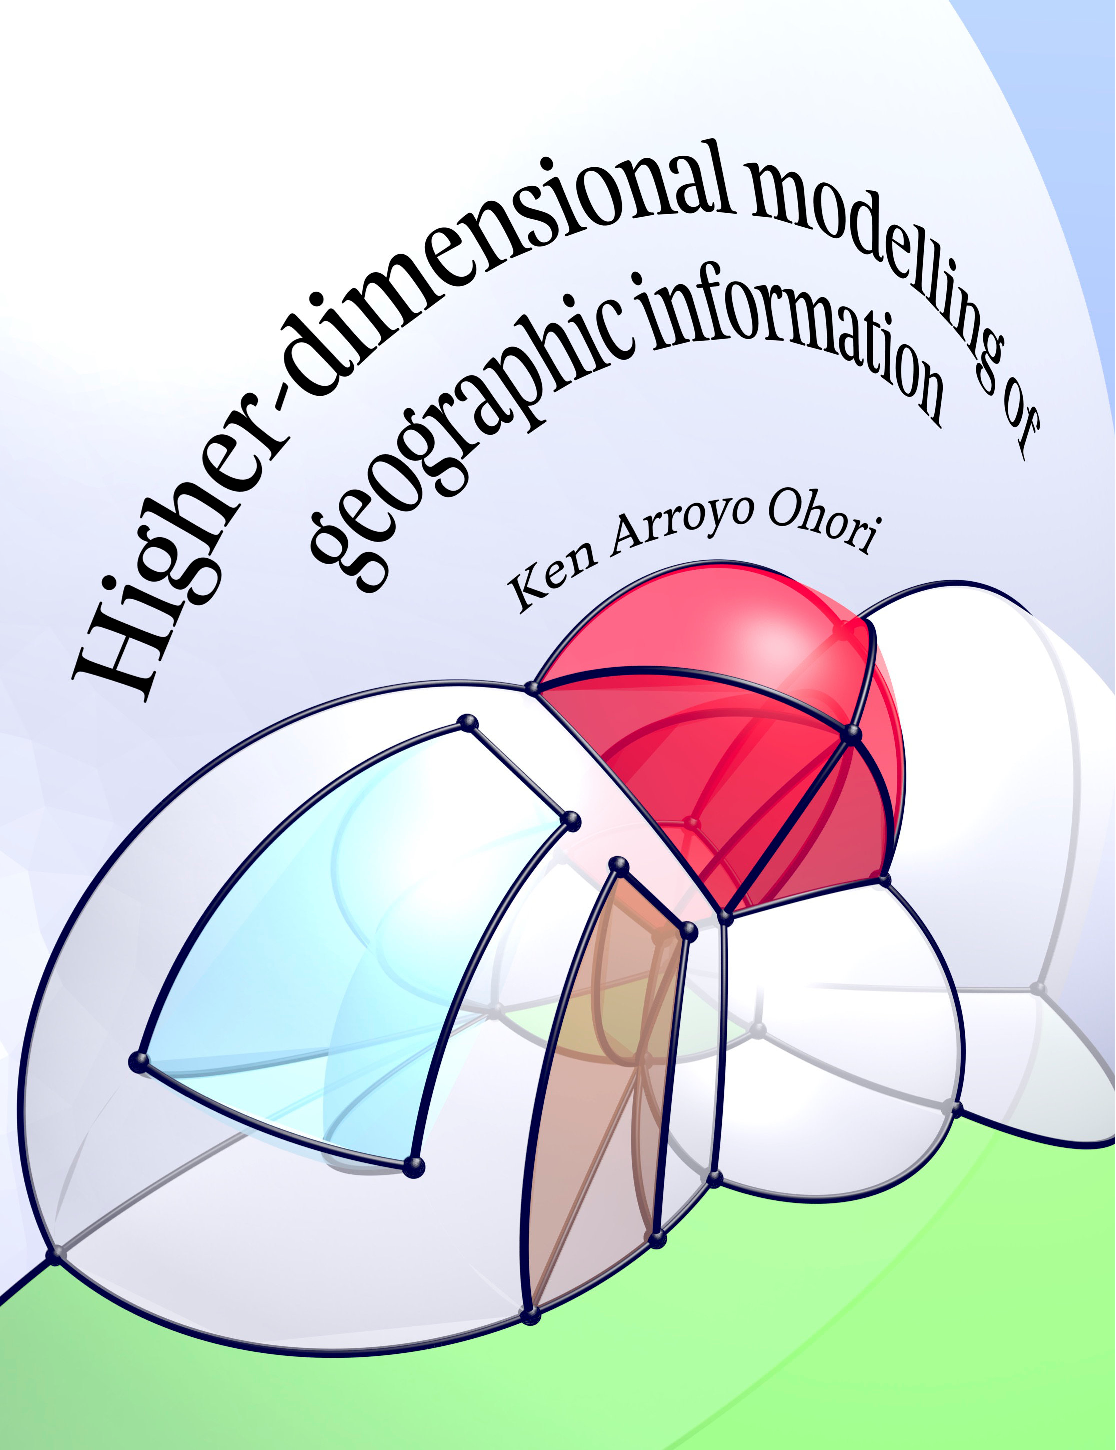
\includepdf{cover-front.pdf}

% Sloppy spacing works better for small paper sizes: better than text outside margin, esp. because of marginpars
\sloppy

\frontmatter

\newgeometry{top=2.170cm,
            bottom=3.510cm,
            inner=2.1835cm,
            outer=2.1835cm,
            ignoremp}
% !TEX root = thesis.tex

% Front cover
% 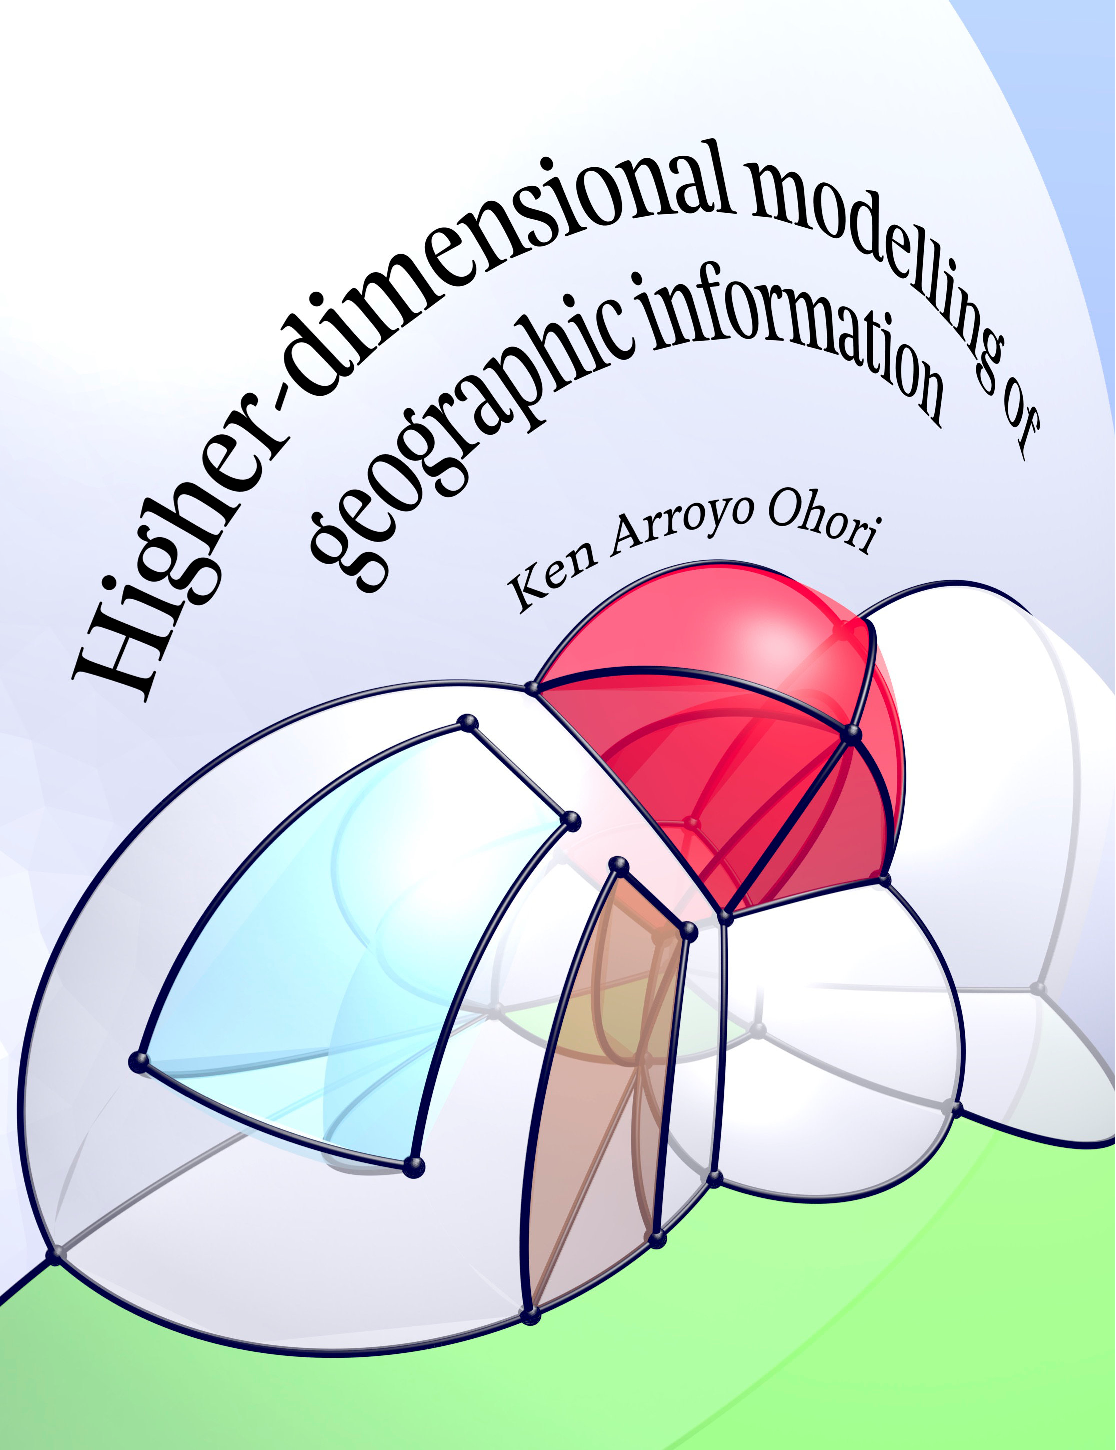
\includepdf{cover-front.pdf}

% Half-title
\author{Ken Arroyo Ohori}
\title{Higher-dimensional modelling of geographic information}
\date{}
\maketitle

% Copyright page
\clearpage
\thispagestyle{empty}
\null%
\label{thesis:colophon}
\vfill
\pdfbookmark[1]{Colophon}{thesis:colophon}
Written in 2014--2016 by
{\makeatletter
\href{http://ken.mx}{\@author}%
\makeatother}.

\textbf{No copyright}\\
\cczero\ This thesis is released into the public domain using the CC0 code.
To the extent possible under law, I waive all copyright and related or neighbouring rights to this work.

To view a copy of the CC0 code, visit: \\
\url{http://creativecommons.org/publicdomain/zero/1.0/}

\textbf{Caveat} \\
I am very happy to release \emph{my own text and figures} without any restrictions whatsoever.
As far as I am concerned, any \emph{attribution is very much appreciated} but it is not required.
However, this does not except anyone from following the academic practices on attribution as applicable to them.
Also, I must note that throughout this thesis I have used several excerpts of others' text, images and code, which I have always been careful to mark as such.
While I am myself allowed to use these excerpts under legal \emph{fair use} doctrines in many countries and more specifically by the citation right (\emph{citaatrecht}) in \href{http://wetten.overheid.nl/jci1.3:c:BWBR0001886&hoofdstuk=I&paragraaf=6&artikel=15a&z=2015-07-01&g=2015-07-01}{Article 15a of the Dutch Copyright Law} (\emph{Auteurswet}), this does not mean that you are also free to use these excerpts for any purpose.

\textbf{Colophon} \\
This thesis was typeset with \XeTeX\ 3.14159265--2.6--0.99992 (\TeX\ Live 2015) using the \mbox{{\fanciestfont{}Feijoa}}, \texttt{GT Pressura} and $\mathrm{Asana\ Math}$ typefaces.
Most of the figures were created using OmniGraffle, Affinity Designer or Blender, often with the help of \LaTeX{}\textsuperscript{i}T.

The source code of this thesis is available at: \\
\url{https://github.com/kenohori/thesis}

\textbf{Cover} \\
Model of a 4D house represented as a 4D cell complex.
The cells of the model were manually defined and embedded in $\mathbb{R}^4$, projected inwards/outwards to the volume of a 3-sphere ($S^3$), stereographically projected to $\mathbb{R}^3$ and exported as an\ {}.obj file.
This was then imported in Blender and rendered using a perspective projection down to 2D.
See \refse{se:4dto3d} for more details.

% Official title
\begin{titlepage}
\null%
\label{thesis:title}
\vspace{3em}%
\pdfbookmark[1]{Title}{thesis:title}
\begin{center}

%% Skip space as in half-title
\vspace*{4\baselineskip}

%% Print the title.
{\makeatletter
\fanciestfont\huge\@title%
\makeatother}
\vfill

%% Apart from the names and dates, the following text is dictated by the
%% promotieregelement.

{\Large Proefschrift}

\medskip

{ter verkrijging van de graad van doctor \\
aan de Technische Universiteit Delft, \\
op gezag van de Rector Magnificus prof.~ir.~K.~C.~A.~M.~Luyben, \\
voorzitter van het College voor Promoties, \\
in het openbaar te verdedigen op \\
6 april 2016 om 12.30 uur}

\medskip

door

\medskip

%% Print the full name of the author.
\makeatletter
{\Large Gustavo Adolfo Ken {\scshape Arroyo Ohori}}
\makeatother

\medskip

Master of Science in Geomatics \\
geboren te Mexico-Stad, Mexico.

\end{center}
\end{titlepage}

% Official verso
\clearpage
\thispagestyle{empty}
\null%
\label{thesis:committee}
\vfill
\pdfbookmark[1]{Doctoral committee}{thesis:committee}

\noindent This dissertation has been approved by the

\medskip\noindent
\begin{tabular}{@{}ll@{}}
  \quad{}promotor: & Prof.\ dr.\ J.\ Stoter \\
  \quad{}copromotor: & Dr.\ H.\ Ledoux \\
\\
\multicolumn{2}{@{}l@{}}{Composition of the doctoral committee:} \\
\\
  \quad{}Rector Magnificus & chairperson \\
  \quad{}Prof.\ dr.\ J.\ Stoter & Delft University of Technology, promotor \\
  \quad{}Dr.\ H.\ Ledoux & Delft University of Technology, copromotor \\
\\
\multicolumn{2}{@{}l@{}}{Independent members:} \\
\\
  \quad{}Prof.\ dr.\ E.\ Eisemann & Delft University of Technology \\
  \quad{}Prof.\ dr.\ M.\ van\ Kreveld & Utrecht University \\
  \quad{}Dr.\ R.\ Lindenbergh & Delft University of Technology \\
  \quad{}Prof.\ dr.\ ir.\ A.\ van\ Timmeren & Delft University of Technology \\ 
\\
\multicolumn{2}{@{}l@{}}{Other member:} \\
\\
  \quad{}Dr.\ G.\ Damiand & Claude Bernard University Lyon 1 \\
\end{tabular}

This research was supported by the Dutch Technology Foundation STW, which is part of the Netherlands Organisation for Scientific Research (NWO), and which is partly funded by the Ministry of Economic Affairs (Project code: 11300).

% No colour links in tables of contents and list of figures
\cleardoublepage%
\tableofcontents
% \cleardoublepage%
\listoffigures
% \cleardoublepage%
% \listoftables
\restoregeometry%

\mainmatter%

% Lengths used for page head
\newlength{\overflowingheadlen}
\setlength{\overflowingheadlen}{\linewidth}
\addtolength{\overflowingheadlen}{\marginparsep}
\addtolength{\overflowingheadlen}{\marginparwidth}

% Page style for preface
\renewpagestyle{scrheadings}{
  {\hspace{-\marginparwidth}\hspace{-\marginparsep}\makebox[\overflowingheadlen][l]{\makebox[2em][r]{\thepage}\quad\rule{1pt}{100pt}\quad{}Preface}}%
  {\makebox[\overflowingheadlen][r]{\rightmark\quad\rule{1pt}{100pt}\quad\makebox[2em][l]{\thepage}}}%
  {}
}{
  {}%
  {}%
  {}
}
\renewpagestyle{plain.scrheadings}{
  {}%
  {}%
  {}
}{
  {\thepage}%
  {\makebox[\overflowingheadlen][r]{\thepage}}%
  {}
}

% !TEX root = thesis.tex

\chapter*{Preface}
% \addcontentsline{toc}{chapter}{Preface}

We usually associate the three usual dimensions with length, width and height (in any order), and the fourth dimension with time. 
However, mathematically, dimensions are essentially a artificial construct and do not have a fixed meaning linked to any specific aspect of reality.
By associating each dimension with a variable, they can be used to represent pretty much anything that we can put a parameter to.
Within this thesis, representations of any dimension are thus used to model various aspects of geographic information, such as the typical geographic coordinates, but also time and scale.

At the end of the 19th century, a couple of non-scientific books were notable for popularising thinking about dimensions, the satyrical \emph{Flatland: A Romance of Many Dimensions} \citep{Abbott84} (\reffig{fig:flatland}), and the more serious \emph{A New Era of Thought} \citep{Hinton88}.
These books used playful analogies between familiar 0D--3D situations and those in higher dimensions, attempting to give readers an intuitive feeling of what these abstract higher dimensions are like.
Plenty of others continue to follow in their footsteps (\reffig{fig:futurama}).

\marginpar{
\captionsetup{type=figure}
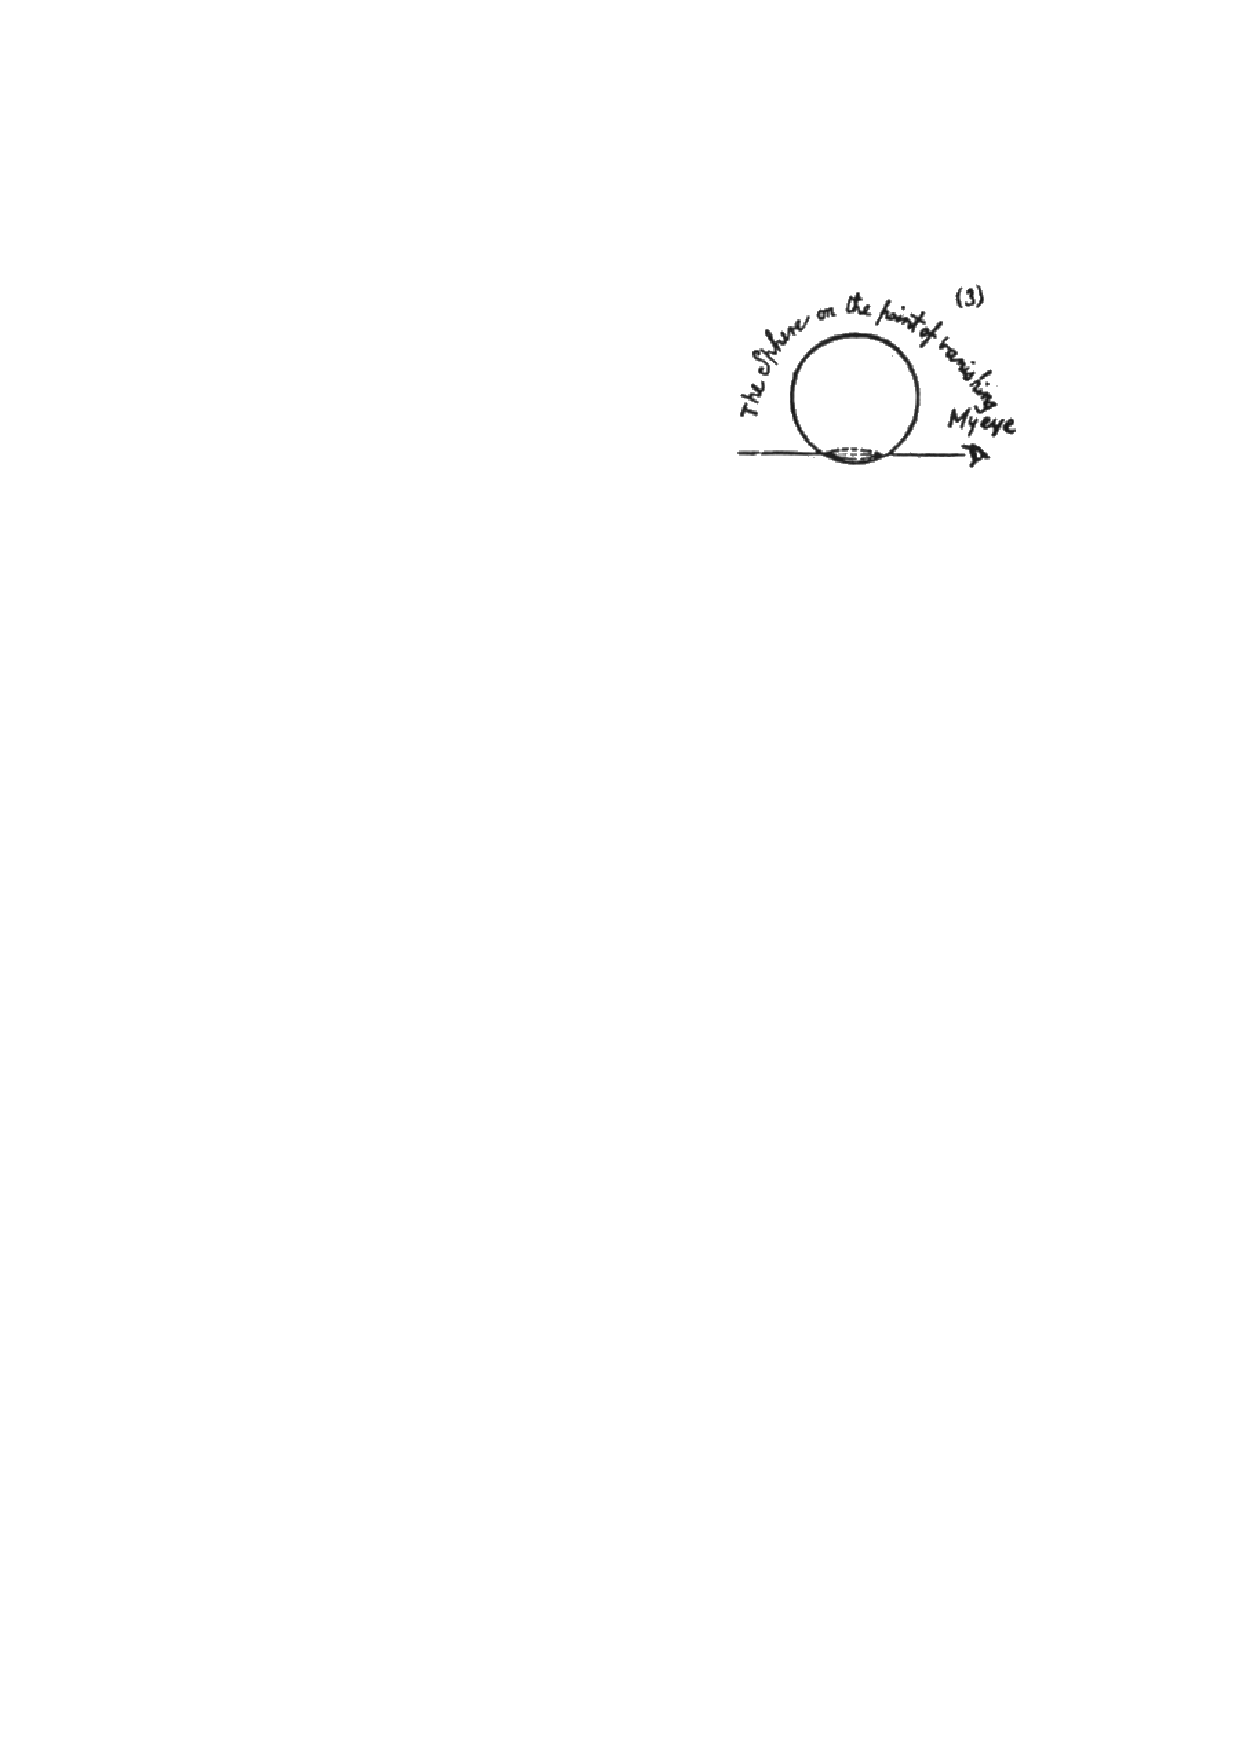
\includegraphics[width=\marginparwidth]{figs/flatland}
\caption[Sphere tries to explain the nature of 3D space to Square]{As Sphere tries to explain the nature of 3D space to Square by passing through its plane of view: `\emph{You cannot indeed see more than one of my sections, or Circles, at a time; for you have no power to raise your eye out of the plane of Flatland; but you can at least see that, as I rise in Space, so my sections become smaller}' \citep{Abbott84}.}
\label{fig:flatland}
}

\marginpar{
\captionsetup{type=figure}
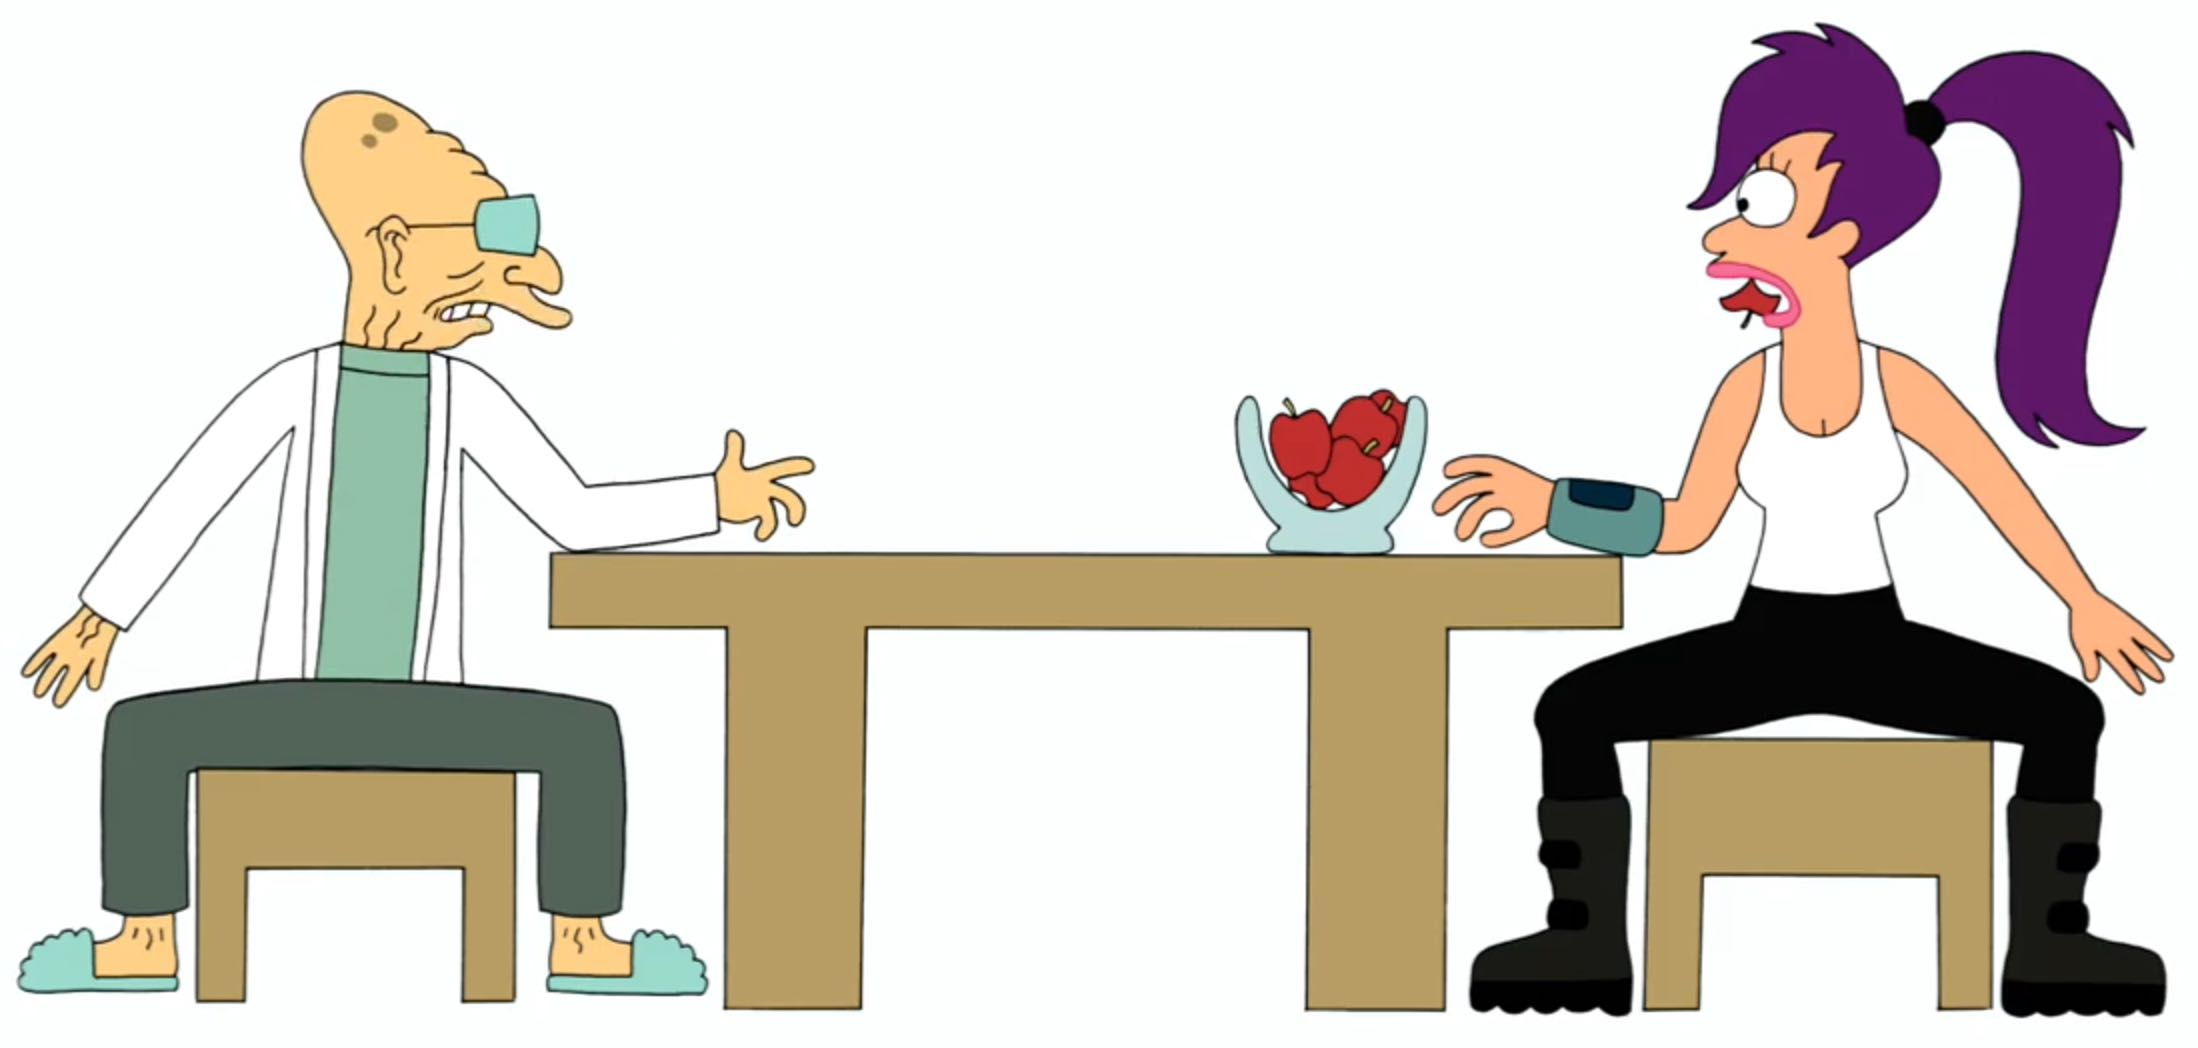
\includegraphics[width=\marginparwidth]{figs/futurama}
\caption[Farnsworth explains why a two-ended digestive system cannot exist in 2D]{As Professor Farnsworth explains why a two-ended digestive system cannot exist in a 2D world: `\emph{As you can see, or rather can't see, but take my word for it, such a digestive system would divide a 2D being into separate pieces.}'. From Futurama season 7 episode 14.}
\label{fig:futurama}
}

In order to ensure that all descriptions are formally correct, this thesis necessarily uses some formal descriptions for its data structures and algorithms.
However, it also tries to provide intuitive explanations and analogies across different dimensions, offering explanations of higher-dimensional problems based on our intuitive knowledge of similar 2D and 3D cases.
I hope that the result is approachable and serves to broach the subject in a practical way, and that potential readers (if any) are not put off by overly technical explanations or by the overly simplistic examples that I am able to draw.

\section*{About this thesis}

During the past 4+ years I have found many things to love about the scientific process, but many things to hate about how its results are released and published.
More than a century after Leo Tolstoy's \emph{Letter to the Free Age Press}\footnote{\url{https://en.wikisource.org/wiki/Letter_to_the_Free_Age_Press}} and 20 years after Stevan Harnad's \emph{subversive proposal}\footnote{\url{https://en.wikipedia.org/wiki/Subversive_Proposal}}, it is rather sad to see that so much science is still kept behind paywalls or stymied by legal restrictions even when it is taxpayer-funded.
% \footnote{Something that is true for much industry research as well, which is paid from tax exemptions on R\&D}.
This is not only damaging to scientific discourse, but it keeps important knowledge from the public at large, including educators and legislators.
% The industry is of course all too glad to fill this void with duplicitous studies, which are often pushed by lobbyists in slick packaging.

At the same time, there is a concerted effort to restrict knowledge creation and creative expression through draconian intellectual property laws, including providing IP holders with special (extra)legal privileges and misappropriating author and user rights while extending already excessive copyright terms.
Plenty of laws have been enacted on the matter with a complete lack of transparency, despite obvious harm to users and evidence to a lack of economic benefits \citep{Hargreaves11,Reda14,EFI15}.
% For all intents and purposes, a system ostensibly created for the protection of authors have been co-opted by the copyright industries.

By releasing this thesis' contents into the public domain and making its source publicly available, I wish to make a small statement about how I believe science should be distributed in the future---openly and without restrictions.
Open access journals are a step in the right direction\footnote{Even as many of them have abusive fees that bear no relation with the marginal cost of internet distribution.}, but I hope it is not too long before we are able to get rid of profit-driven journals and publishers altogether.

Following in the same spirit, the source code of the main prototype implementations that were developed during this PhD project have also been made publicly available under permissive licences, which are linked to in the corresponding parts of this thesis.
As others have pointed out before me\footnote{See for instance \citet{Morin12}, \citet{Joppa13} and \citet{Ince12}}, there is a great disparity between the alleged importance of scientific evidence and widespread acceptance of not disclosing software implementations.
% More cogently, \emph{there is no such thing as reproducibility without source code}.

\section*{Acknowledgements}

My utmost thanks go to my supervisors, \textbf{Hugo} and \textbf{Jantien}.
They not only provided me with \emph{years} of employment and the wonderful opportunity to work on this PhD, but were always there with good ideas, and all the guidance and support anyone could ever wish.
I am also very grateful to \textbf{Guillaume} for hosting me in Lyon and helping me to understand the details of his CGAL packages, which were used in large parts of this thesis.

Special thanks go to everyone else in the \textbf{3D geoinformation} group during my time there (\textbf{Filip}, \textbf{Liu}, \textbf{Ravi}, \textbf{Sisi} and \textbf{Zhiyong}).
It is truly a fantastic place to work and I feel privileged to have been able to contribute to it with my grain of sand.

I am also thankful to everyone at \textbf{GIS technology} (\textbf{Edward}, \textbf{Elfriede}, \textbf{Marian}, \textbf{Martijn}, \textbf{Peter}, \textbf{Radan}, \textbf{Theo}, \textbf{Tjeu}, and \textbf{Wilko}).
Many of them gave me insightful comments and support, especially so for Peter at the start of this PhD.

Last but not least, I especially thank my mother, \textbf{Kimiyo}, who has always been there supporting me, and my \textbf{close friends} in Mexico, the Netherlands and elsewhere, who made sure I always had things to enjoy outside work.
I could not mention you all by name without making a dubious classification, which I do not want to do, and so I hope you will forgive me for just refusing to do so.
\emph{Thank you all}.

% Page style for chapters
\renewpagestyle{scrheadings}{
  {\hspace{-\marginparwidth}\hspace{-\marginparsep}\makebox[\overflowingheadlen][l]{\makebox[2em][r]{\thepage}\quad\rule{1pt}{100pt}\quad{}\leftmark}}%
  {\makebox[\overflowingheadlen][r]{\rightmark\quad\rule{1pt}{100pt}\quad\makebox[2em][l]{\thepage}}}%
  {}
}{
  {}%
  {}%
  {}
}
\renewpagestyle{plain.scrheadings}{
  {}%
  {}%
  {}
}{
  {\thepage}%
  {\makebox[\overflowingheadlen][r]{\thepage}}%
  {}
}

% !TEX root = thesis.tex

\chapter{Introduction}
\label{ch:introduction}

% Spatial information

\emph{Spatial information} describes the location of objects in space and the relationships between them.
Within this thesis the emphasis is on \emph{geographic} information as represented in a \emph{computer}, which uses similar techniques but narrows this definition to information that is about the real world and at a human-to-Earth scale, using abstracted digital representations of real-world entities such as terrain, cities, roads and buildings.
These entities and the relationships between them are defined using sets of interlinked computer primitives.
Because of this, spatial information forms a necessary component of any computer model of the world as we know it at any significant level of detail.

% GIS research

At the core of this subject lies the research on \emph{geographic information systems (GIS)}, which produces tools to create, manipulate, analyse and view the digital objects that are inherent in these abstract representations of the world.
Compared to other software categories that also work with geometric objects, such as those used in computer-aided design (CAD) and geometric modelling, GIS tools stand out as being remarkably \emph{generic}.
They are used equally to manually model objects by interactively drawing primitives, to semi-automatically create models from raw acquired data, to manage large collections of heterogeneous datasets and keep them up to date, or as interactive environments to query the attributes of and perform simple calculations on existing datasets.
Because of this genericity, GIS tools are expected to support a large number of different data formats from multiple sources and a wide variety of operations---all while solving problems in both 2D and 3D and preserving the key characteristics of sometimes incompatible computer representations.
\emph{Rather than guaranteeing the best solution on input fulfilling certain strict conditions, GIS tools are  expected to make a best effort to obtain a good solution on the (often messy) data that is available}.

% 2D representations in GIS

For historical and practical reasons, current GIS mostly use simple 2D representations \citep{ESRITopology,SimpleFeatures1}, which are relatively easy to use and efficient, essentially consisting of sets of linked points, lines and polygons.
Their efficiency is due to the fact that they can rely on many strong properties that are intrinsic to 2D objects.
For example, one such property is that it is possible to define a natural order for the points around a closed polygonal curve, as shown in \reffig{fig:loop},
\marginpar{
\captionsetup{type=figure}
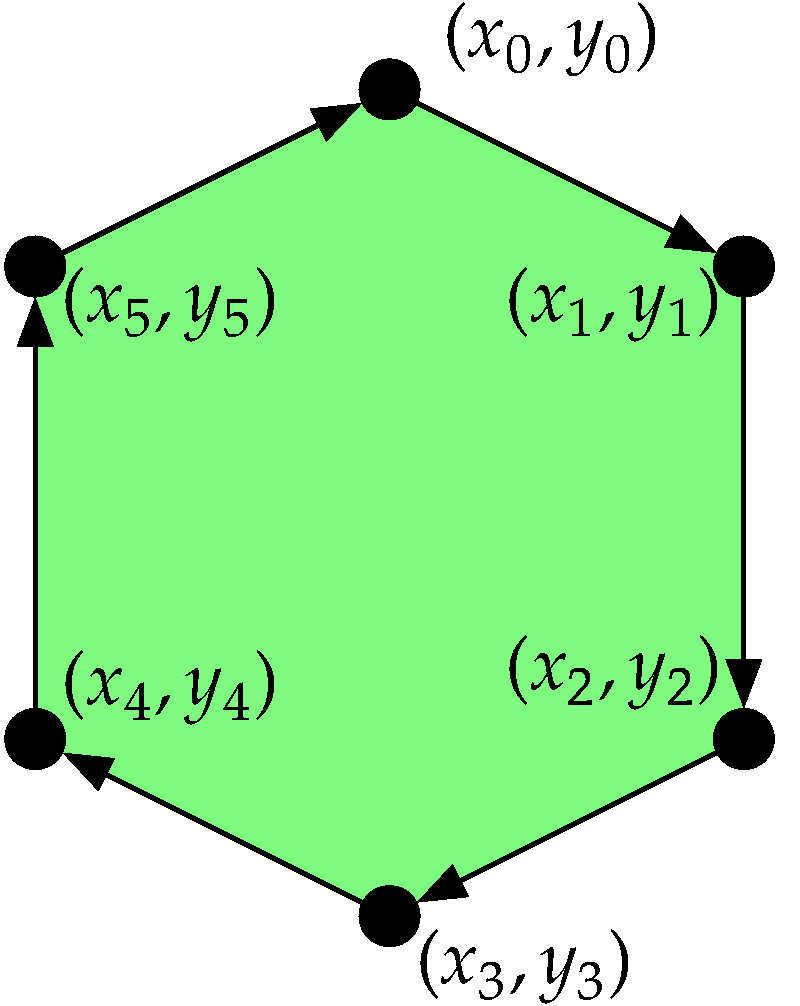
\includegraphics[width=\marginparwidth]{figs/loop}
\caption{A polygon as a cycle of points}
\label{fig:loop}
}
and so a polygon can be represented as a sequence of points that form a cycle along its boundary \citep{Jordan87}, which are implicitly connected by line segments between each consecutive pair.
Another such property is based on planar partitions---sets of polygons that form a subdivision of the plane---such as the one in \reffig{fig:corine}.
\marginpar{
\captionsetup{type=figure}
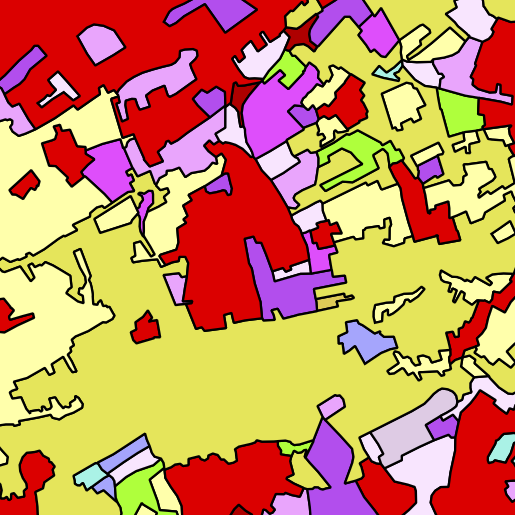
\includegraphics[width=\marginparwidth]{figs/corine}
\caption[The polygons in the CORINE dataset around Delft]{The polygons in the CORINE\protect\footnotemark\ dataset in the area around Delft \citep{CEC95}}
\label{fig:corine}
}
\footnotetext{\url{http://www.eea.europa.eu/publications/COR0-landcover}}
Since in a planar partition there are two polygons incident to any edge (except those bordering the exterior), a complete planar partition can be stored easily as a set of edges where every edge is linked to two other edges and records the polygons that lie on each of its two sides \citep{Peucker75}.

% 2D operations -> slowly start with problem

2D GIS are also able to take advantage of a great number of existing techniques that are based on 2D representations, such as those that are used to model the flow of water over a terrain \citep{vanKreveld97} or to combine multiple maps into one (\ie\ a map overlay) \citep[\S{}2.3]{deBerg08}.
Moreover, these techniques have been developed and improved over decades, whereas any change in representation would require the development of new accompanying techniques in order to be truly useful.

% 3D? Not really
% TODO: Weird space between the figures above and below in list of figures

The aforementioned advantages of 2D representations mean that even `3D' GIS usually mimic the third dimension by using a so-called 2.5D structure, essentially treating the third dimension as a simple attribute that is attached to each object \citep{Raper89}, or represent individual 3D objects only implicitly through the 2D surface that separates their interior from their exterior \citep{Edmonds60,Baumgart75}, as the cube in \reffig{fig:brep}, rather than as true solid objects.
\marginpar{
\captionsetup{type=figure}
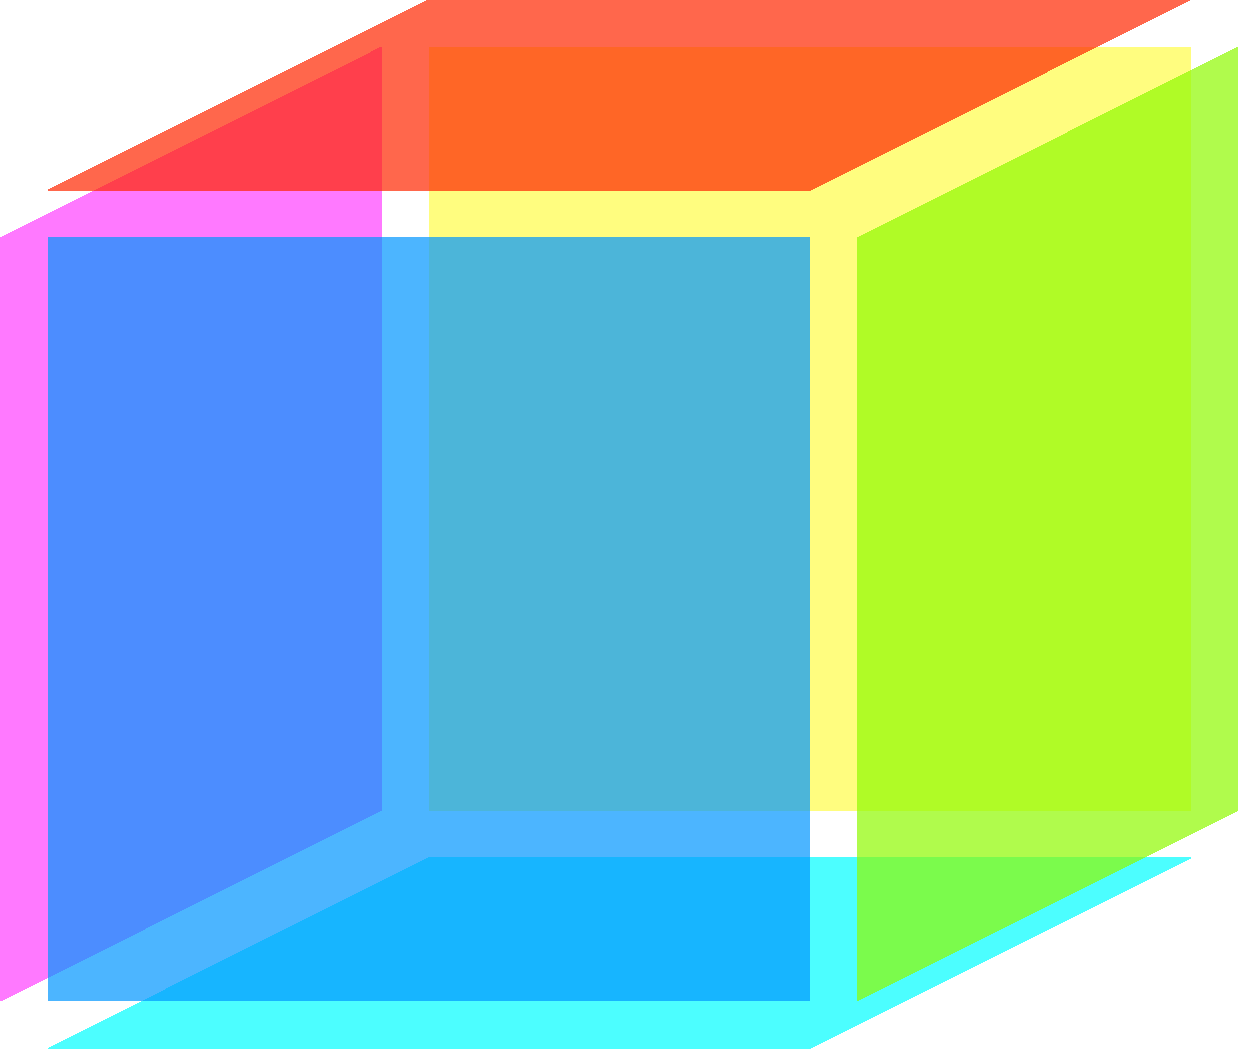
\includegraphics[width=\marginparwidth]{figs/brep}
\caption{A cube represented as the 6 square faces that bound it}
\label{fig:brep}
}
These solutions are compromises, as they limit the type of geometries that can be represented and complicate the storage of the relations that exist between 3D objects.

% Time/scale, also 2D

Another important consequence is that when non-spatial characteristics that have a strong link to space, such as time and scale, are integrated in a GIS, they are usually implemented using similar adaptations of 2D representations.
For example, spatiotemporal GIS keep multiple representations of 2D structures \citep{Armstrong88}, each at a different point in time, or a list of changes per object \citep{Worboys92,Peuquet94}, while multi-scale datasets generally consist of independent datasets for each scale with some common identifiers that link objects between datasets \citep{Friis-Christensen03,Stoter14}.

% Limits 3D operations

The use of 2D representations also limits the capabilities of GIS software, as the techniques that can be implemented on top of these 2D representations cannot make full use of the potential of 3D spatial information \citep[Ch.~3]{Zlatanova00}.
For instance, current GIS are largely unable to manipulate 3D objects or to compute geometric operations between multiple 3D objects, forcing users to perform such functions in 3D modelling software.
These examples are notable as similar functionality for is widespread in 2D GIS and expected by users.

% nD approach -> solution

A potential solution to these problems is to represent certain parametrisable characteristics as additional dimensions in the geometric sense, as shown in \reffig{fig:axes}, such that real-world entities are modelled as higher-dimensional objects embedded in higher-dimensional space \citep{vanOosterom10}.
\marginpar{
\captionsetup{type=figure}
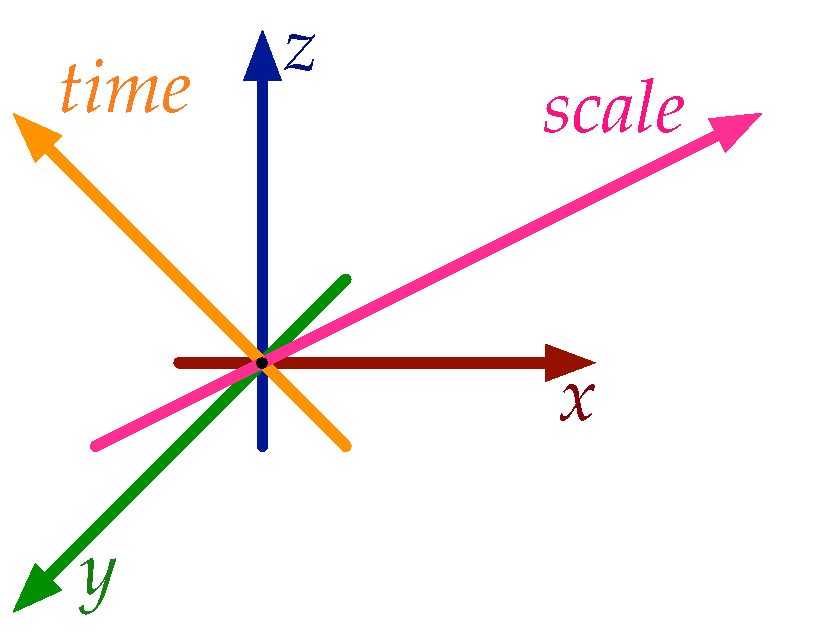
\includegraphics[width=\marginparwidth]{figs/axes}
\caption{Five dimensions based on 3D space, time and scale}
\label{fig:axes}
}
A building existing over a time span and stored at a range of scales on a computer could thus be represented as a single 5D object.

% Why?

This \emph{higher-dimensional geographic information modelling} approach is well grounded in long-standing mathematical theories, such as the setting of coordinates to space \citep{Descartes37}, and theories of higher-dimensional geometry \citep{Riemann68} and topology \citep{Poincare95}.
It also opens the door for new, more powerful techniques and practical applications.
For example, these $n$-dimensional representations could be used to ensure that an object is consistent along all dimensions (\eg\ a building at different points in time or levels of detail), or to analyse its relations to other objects along all dimensions as well.

% Scientific gap

While there is a large body of related work on the representation of abstract $n$-dimensional objects in mathematics and computer science \citep{Brisson93,Lienhardt94}, it is necessary to extend these representations to make them fit for use with real-world objects, which have aspects that are difficult to handle in certain idealised representations, \eg\ certain complex geometries (\reffig{fig:nonmanifold})
\marginpar{
\captionsetup{type=figure}
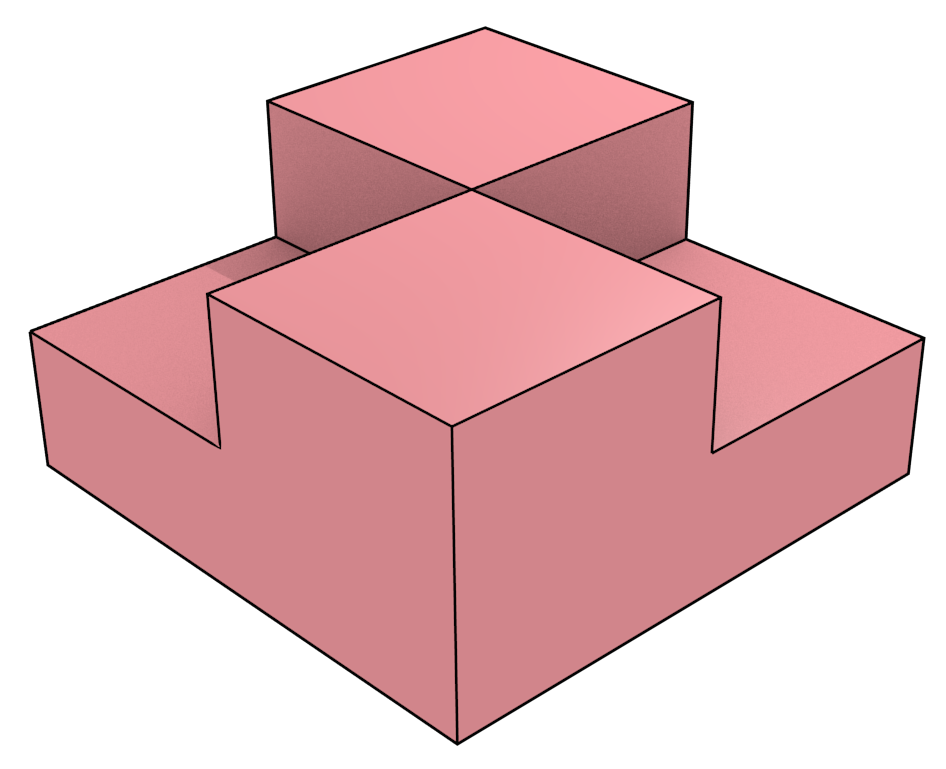
\includegraphics[width=\marginparwidth]{figs/nonmanifold}
\caption[A non-manifold shape]{This non-manifold shape cannot be handled properly in many representations.}
\label{fig:nonmanifold}
}
, holes (\reffig{fig:torus})
\marginpar{
\captionsetup{type=figure}
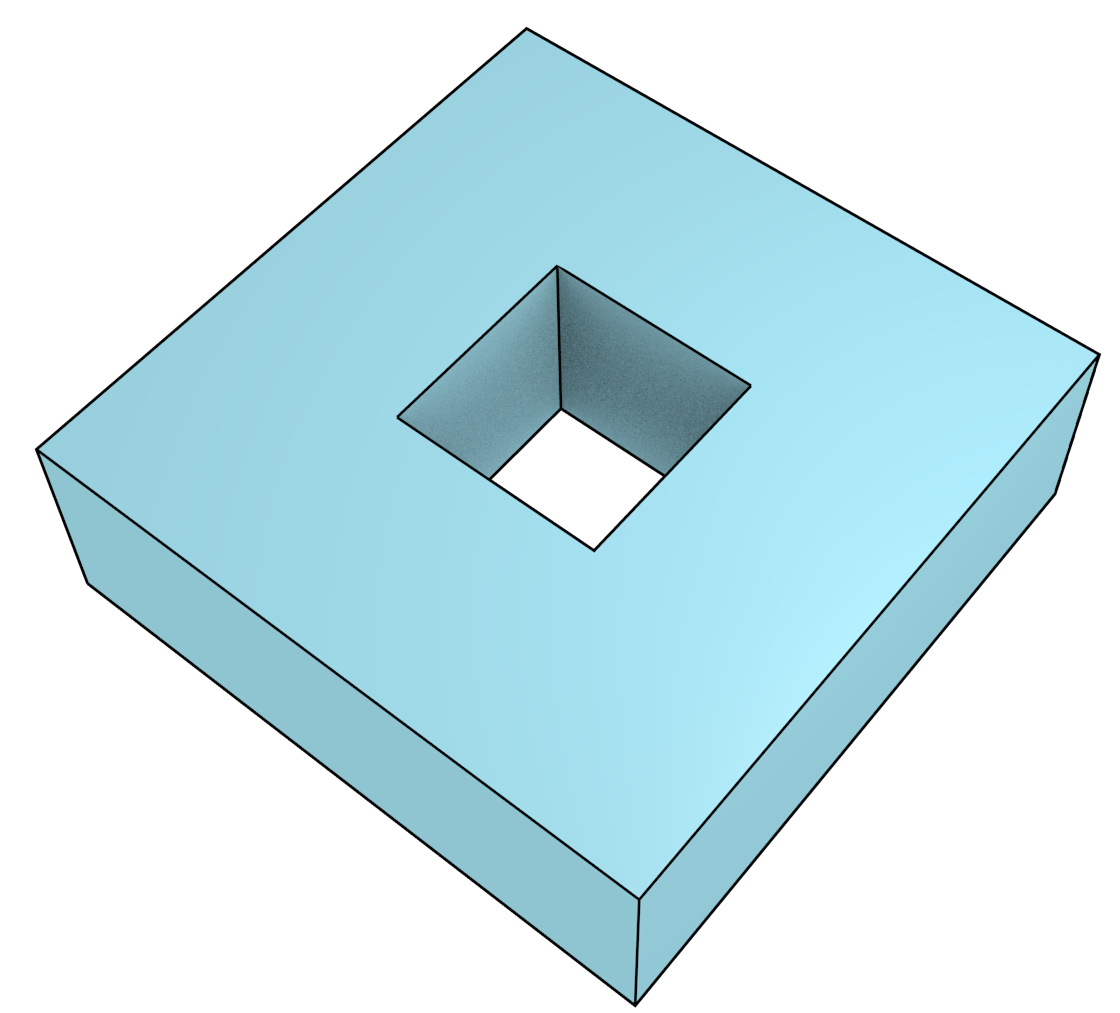
\includegraphics[width=\marginparwidth]{figs/torus}
\caption{The top and bottom faces of this torus have holes in them.}
\label{fig:torus}
}
and semantics.
Additionally, making this approach attractive in practice requires the development of techniques to construct, analyse and visualise higher-dimensional geographic objects.
Finally, there are significant technical issues involved in the realisation of these representations and techniques into a computer implementation.

\section{Research objective and scope}
\label{se:objective}

In order to determine whether the higher-dimensional modelling approach is worthwhile, and if so, the conditions under which it makes sense to follow it, it is necessary to gain a greater understanding of the entire modelling process and its technical consequences.
The main aim of this thesis is therefore to gain this understanding by \textbf{realising the fundamental aspects of a higher-dimensional Geographic Information System}, ranging from the development of the necessary concepts to the creation of prototype-level working software using real-world higher-dimensional datasets.
In this sense, I purposefully do not intend to prove that the higher-dimensional spatial modelling approach is better or worse than existing approaches, but instead to highlight its advantages and disadvantages.

\section{Structure of this thesis}
\label{se:about}

This thesis comprises two main parts, each of which contains a few chapters and which respectively cover methods to solve problems inherent in: (i) representing objects in arbitrary dimensions, and (ii) creating and manipulating such objects.
After these, there are some independent chapters falling outside these parts, covering ancillary aspects and putting together the results of the rest.
All chapters are described in detail below.

% \clearpage

\begin{description}

% Part I
% \textbf{\refpa{pa:representation} \nameref{pa:representation}}
\item[\refpa{pa:representation} \nameref{pa:representation}] \ 

\begin{description}

\item[\refch{ch:modelling-mathematics}]
introduces the mathematical concepts and background behind spatial data modelling.

\item[\refch{ch:modelling-background}]
describes and analyses the state of the art in the 2D and 3D modelling of space, time, scale and attributes.
% , doing so with a view to possible higher-dimensional extensions.
It concludes by listing some of the shortcomings of current approaches.

\item[\refch{ch:nd-modelling}]
presents the higher-dimensional modelling paradigm that is the basis of this thesis, which aims to solve many of the problems alluded to in \refch{ch:modelling-background}.
It also describes and evaluates the higher-dimensional representations that can be used in order to realise this approach, which take the form of $n$-dimensional data models and structures.

\end{description}

% Part II
% \textbf{\refpa{pa:operations} \nameref{pa:operations}}
\item[\refpa{pa:operations} \nameref{pa:operations}] \ 

\begin{description}

\item[\refch{ch:operations-background}]
presents a few fundamental operations for some of the data structures described in \refch{ch:nd-modelling}.
These are used in order to build the higher level operations described in the other chapters within \refpa{pa:operations}.

\item[\refch{ch:extrusion}]
describes $n$-dimensional extrusion, an extension of the well-known 2D to 3D extrusion operator in GIS.\@
It can be used to generate simple prism-shaped $n$-dimensional objects from an $(n-1)$-dimensional space partition by assigning to each $(n-1)$-dimensional object a range along which it exists.

\item[\refch{ch:incremental-construction}]
describes incremental construction, an operation which is able to generate arbitrary $n$-dimensional objects based on defining their $(n-1)$-dimensional boundary.
It is equivalent to the generation of the topological relationships that exist between a set of $(n-1)$-dimensional objects.

\item[\refch{ch:linking-lods}]
shows how a higher level construction operator that links a series of 2D or 3D models can be created.
This enables the construction of 4D models from real-world 3D city models covering the same region.

\item[\refch{ch:slicing}]
explains how 2D and 3D information can be extracted from a higher-dimensional representation by selecting appropriate portions of the data (\eg\ cross-sections) and projecting it to 2D/3D space.

\end{description}

% \bigskip
% \textbf{\refpa{pa:implementation} \nameref{pa:implementation}}
% \begin{description}

\item[\refch{ch:cleaning}]
explains the main data validation and repair techniques that are used to create 2D/3D/$n$D objects and space partitions out of real-world GIS datasets, which often have defects that impede their usage.
By obtaining clean geometric models, these techniques enable the use of the higher-dimensional modelling approach in practice.

% \end{description}

% Conclusions
% \bigskip
\item[\refch{ch:conclusions}]
concludes this thesis by explaining the achievements of this PhD project and highlighting the main challenges to further develop a higher-dimensional GIS.\@
It contains an outlook on how higher-dimensional modelling can be used in GIS as well as some suggestions for future work.

\item[\refap{ch:implementation}]
describes the most relevant implementation details concerning the representations and operations from the previous chapters, such as the use of various software libraries,  programming techniques.

\item[\refap{ch:dictionary}] 
contains a short dictionary of terms for higher-dimensional GIS.\@
As the terminology used in 2D GIS, 3D GIS, CAD, geometric modelling and other related fields can be different and is often used inconsistently and rather loosely, the appendix is intended for use as reference and for the better understanding of the thesis.

\end{description}


\setpartpreamble{
  \vspace{3cm}
  \begin{center}
  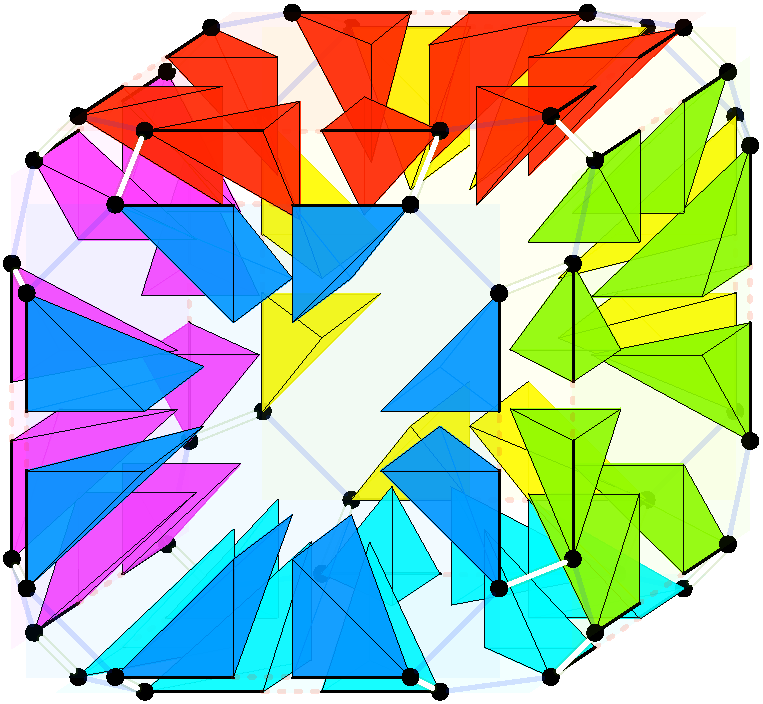
\includegraphics[width=0.8\linewidth]{figs/gmaps-3d-simplices}
  \end{center}
}
\newgeometry{top=2.170cm,
            bottom=3.510cm,
            inner=2.1835cm,
            outer=2.1835cm,
            ignoremp}
\part{Representing geographic information}
\label{pa:representation}
\restoregeometry%
% The underlying 3D simplicial complex in the representation of a cube as a 3D generalised map.

% !TEX root = thesis.tex

\chapter{Mathematical foundations of spatial modelling}
\label{ch:modelling-mathematics}

Spatial modelling has its origins in the geographical notion of space, which is in turn based on our own observations of the world and empirical experience \citep{Couclelis99}.
However, these informal notions are error-prone and differ from person to person.
In order to describe space unambiguously, people have thus turned to models that still describe geographical phenomena, but do so using formal notions derived from mathematics.
These formal models make it possible to create and store digital representations of the world in a computer, and thus to use the power of a computer to easily solve spatial problems \citep{Burrough86,Bailey95}.

The current chapter describes some of these formal notions and their relevant context, which are used to study the spatial modelling approaches presented in the upcoming chapters.
\refse{se:settheory} introduces some concepts of elementary set theory and mathematical logic, which are later used in definitions in this thesis.
\refse{se:geometry} introduces the basic concepts of geometry, which are used to describe the position, shape and orientation of objects.
\refse{se:topology} builds on these to present topology, which formalises notions such as the boundary and interior of an object or the relationships between multiple objects.

\section{Elementary set theory and mathematical logic}
\label{se:settheory}

Set theory is the branch of mathematics that studies \emph{sets}, which are collections of abstract objects.
While the study of set theory only formally started with \citet{Cantor74}, its intuitive and minimal concepts were later used in order to give a foundation to almost all areas of mathematics\footnote{Even as some mathematicians and philosophers have argued against set theory as a foundation for all of mathematics.}.
Since the basic concepts of set theory are used in this thesis in order to describe many other concepts, this section gives a very short primer using the same notation that is used in this thesis.
However, it is worth noting that the descriptions used here are reflect the concepts generally used in GIS, and so are meant to be intuitive and not very formal.
Perhaps more importantly, these definitions do not reflect modern mathematical thought on the topic\footnote{In short, these intuitive definitions pretty much assume that anything can be put into a set without leading to paradoxes, which formally is not the case.}, which is much more precise but also less accessible, \eg\ axiomatic set theory.

Set theory starts by considering the existence of a given domain of objects from which one may build sets, which is known as the \emph{universe set} and denoted as $\mathbb{U}$.
These objects can be anything, including other sets.
Set theory allows sets to be regarded as single entities and operated upon \citep{Devlin93}.
If an object $a$ is part of a set $\mathbb{X}$, it is denoted as $a \in \mathbb{X}$, read as `$a$ is an \emph{element} of $\mathbb{X}$'.
If $a$ is not part of a set $\mathbb{X}$, it is denoted as $a \notin \mathbb{X}$, read as `$a$ is not an element of $\mathbb{X}$'.

There are two broad ways to describe the elements in a set, both using curly braces, \ie\ \{ and \}.
One way to do so is to enumerate all the elements of the set one by one.
For instance, the set $\left\{ 1,2,3 \right\}$ is the set containing $1$, $2$ and $3$ as elements (and no others).
The other way to do so is to specify one or more rules that the elements of the set need to fulfil.
For instance, the set $\{ x \mid x$~\emph{is~a~prime~number}$\}$ consists of all prime numbers.
It is read as `$x$, such that $x$ is a prime number'.

Sets are by definition unordered and contain unique elements---duplicate items are ignored by convention.
A set may contain an infinite number of elements (\eg\ as the prime number example above), or no elements at all, in which case it is a special set known as the \emph{null set} and denoted as $\{ \}$ or $\emptyset$.
Other commonly used sets with a special notation and name are: the natural numbers ($\mathbb{N}$), the real numbers ($\mathbb{R}$), the rational numbers ($\mathbb{Q}$) and the integers ($\mathbb{Z}$).

In order to build more complex sets, the concepts and notation from mathematical logic are used, in particular \emph{propositional logic}.
Propositional logic works with \emph{propositions}, which are sentences that are either true or false, but not both.
These propositions might be altered and combined using various symbols expressing various notions, such as: \emph{and} ($\wedge$), \emph{or} ($\vee$), \emph{not} ($\neg$), \emph{implies} ($\Rightarrow$), \emph{is implied by} ($\Leftarrow$), \emph{if and only if} ($\Leftrightarrow$), \emph{for all} ($\forall$) and \emph{exists} ($\exists$).

Using these concepts it becomes possible to state relationships between sets.
For instance, $\mathbb{A}$ and $\mathbb{B}$ are then equal ($\mathbb{A} = \mathbb{B}$) when an element is in $\mathbb{A}$ if and only if it is also in $\mathbb{B}$, which can be denoted as $\forall x : x \in \mathbb{A} \Leftrightarrow x \in \mathbb{B}$.
A set $\mathbb{A}$ is called a subset of a set $\mathbb{B}$ ($\mathbb{A} \subseteq \mathbb{B}$), or $\mathbb{B}$ is a superset of $\mathbb{A}$ ($\mathbb{B} \supseteq \mathbb{A}$), when if an element is in $\mathbb{A}$ then it is also in $\mathbb{B}$, denoted as $\forall x : x \in \mathbb{A} \Rightarrow x \in \mathbb{B}$.
If $\mathbb{A} \subseteq \mathbb{B}$ but $\mathbb{A} \neq \mathbb{B}$, \ie\ there is at least one extra element in $\mathbb{B}$, then $\mathbb{A}$ is a proper subset of $\mathbb{B}$ ($\mathbb{A} \subset \mathbb{B}$), or alternatively $\mathbb{B}$ is a proper superset of $\mathbb{A}$ ($\mathbb{B} \supset \mathbb{A}$).

It is also possible to use propositional logic to create new sets by defining certain operations between sets, in particular \emph{Boolean set operations}, consisting of intersection, union, difference and complement\footnote{These are the most commonly described basic operations. However, it is possible to define other operations that are equally useful as a base. Either can be used to form other operations by composition.}.
The intersection of the sets $\mathbb{A}$ and $\mathbb{B}$, denoted as $\mathbb{A} \cap \mathbb{B}$, consists of all the elements that are both in $\mathbb{A}$ and in $\mathbb{B}$, \ie\ $\mathbb{A} \cap \mathbb{B} = \left\{ x \mid x \in \mathbb{A} \wedge x \in \mathbb{B} \right\}$.
The union of the sets $\mathbb{A}$ and $\mathbb{B}$, denoted as $\mathbb{A} \cup \mathbb{B}$, consists of all the elements that are either in $\mathbb{A}$ or in $\mathbb{B}$, \ie\ $\mathbb{A} \cup \mathbb{B} = \left\{ x \mid x \in \mathbb{A} \vee x \in \mathbb{B} \right\}$.
The difference between sets $\mathbb{A}$ and $\mathbb{B}$, denoted as $\mathbb{A} - \mathbb{B}$, consists of all the elements that are in $\mathbb{A}$ but not in $\mathbb{B}$, \ie\ $\mathbb{A} - \mathbb{B} = \left\{ x \mid x \in \mathbb{A} \wedge x \notin \mathbb{B} \right\}$.
The complement of a set $\mathbb{A}$, denoted as $\neg \mathbb{A}$, consists of all the elements that are in the universe set but are not in $\mathbb{A}$, \ie\ $\neg \mathbb{A} = \left\{ x \mid x \in \mathbb{U} \wedge x \notin \mathbb{A} \right\}$.

Apart from sets, it is also possible to consider \emph{tuples} of elements, which unlike sets are sequences of ordered elements.
A tuple containing exactly two elements is known as a \emph{pair}, one containing three elements is a \emph{treble} and one containing $n$ elements is an $n$-tuple.
Tuples are denoted using parenthesis, \ie\ (\ and~).

A common operation that generates tuples is the Cartesian product.
The Cartesian product of sets $\mathbb{A}$ and $\mathbb{B}$, denoted as $\mathbb{A} \times \mathbb{B}$, is defined as $\left\{ (a,b) \mid a \in \mathbb{A} \wedge b \in \mathbb{B} \right\}$.
In other words, it is a set of pairs, where the first element of a pair is an element of $\mathbb{A}$ and the second element of the pair is an element of $\mathbb{B}$.
This can be generalised to more than two sets, such that the $n$-fold Cartesian product of $n$ sets is an $n$-tuple.
The $n$-fold Cartesian product of a set $\mathbb{A}$ with itself, \ie\ $\mathbb{A} \times \mathbb{A} \times \ldots \mathbb{A}$, is denoted as $\mathbb{A}^n$.

\section{Geometry}
\label{se:geometry}

Geometry is the branch of mathematics concerned with the position of objects in space, a topic that was already formalised by the ancient Greek mathematician Euclid in his textbook \emph{the Elements} around 300 BCE \citep{Fitzpatrick08}.
Euclidean geometry consists of a small set of geometric axioms considered to be intuitively obvious, such as the fact that it is possible to draw exactly one line that passes through two points (\reffig{fig:line}), as well as a long series of postulates derived from these and which describe more complex constructions\footnote{Non-Euclidean geometry does away with some of these axioms while remaining self-consistent \citep{Bolyai32,Lobachevsky40}. However, it is much less relevant in the context of spatial modelling.}.
\marginpar{
\captionsetup{type=figure}
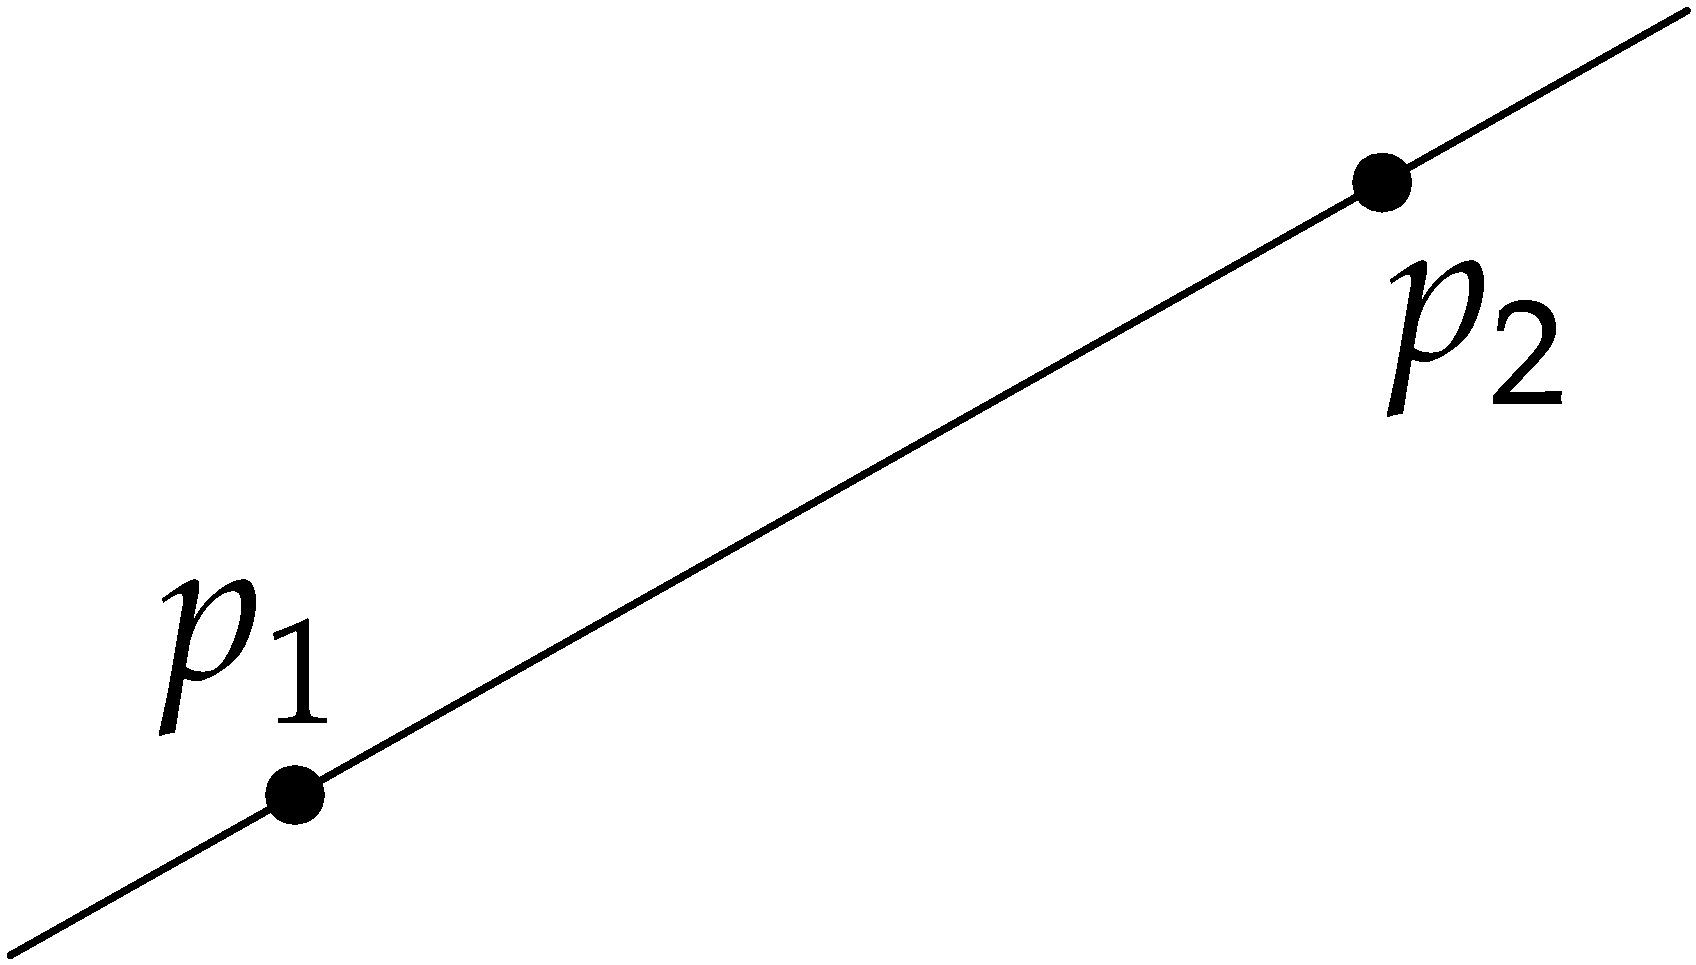
\includegraphics[width=\marginparwidth]{figs/line}
\caption[A single line passes through two points]{There is exactly one line that passes through any pair of points.}
\label{fig:line}
}

However, even as Euclidean geometry has the notions of relative distances, angles and areas, objects in Euclidean geometry do not have an absolute position in space.
Analytic or Cartesian geometry, developed by \citet{Descartes37} and \citet{de-Fermat79}, significantly changed this by introducing the concept of coordinates.
A coordinate system makes it possible to uniquely describe the absolute location of a point as a tuple of real numbers.
In particular, the Cartesian coordinate system uses a tuple of perpendicular directed lines as axes, with a positive direction and a negative direction, all of which intersect at a common point known as the origin.
A point's coordinates in the system are then given by signed distances to the respective axes\footnote{A more rigorous and correct explanation would be based on a set of linearly independent vectors, but this creates a recursive definition.}.

$n$-dimensional Euclidean space, which can be described by the set of points $\mathbb{R}^n$, has $n$ perpendicular axes intersecting at the origin $O$, defined by the $n$-tuple $(0, 0, \ldots, 0)$, and a point $p$ in $n$D space is thus described by an $n$-tuple $(p_1, p_2, \ldots, p_n)$, where $p_i$ is the signed distance to the $i$-th axis.
For example, as shown in \reffig{fig:point}, three-dimensional Euclidean space ($\mathbb{R}^3$), has three axes, usually named $X$, $Y$ and $Z$, such that a given point $p$ in 3D can be described by a treble $(p_x,p_y,p_z)$, where $p_x$ is the signed distance to the $X$ axis, $p_y$ to the $Y$ axis and $p_z$ to the $Z$ axis.
\marginpar{
\captionsetup{type=figure}
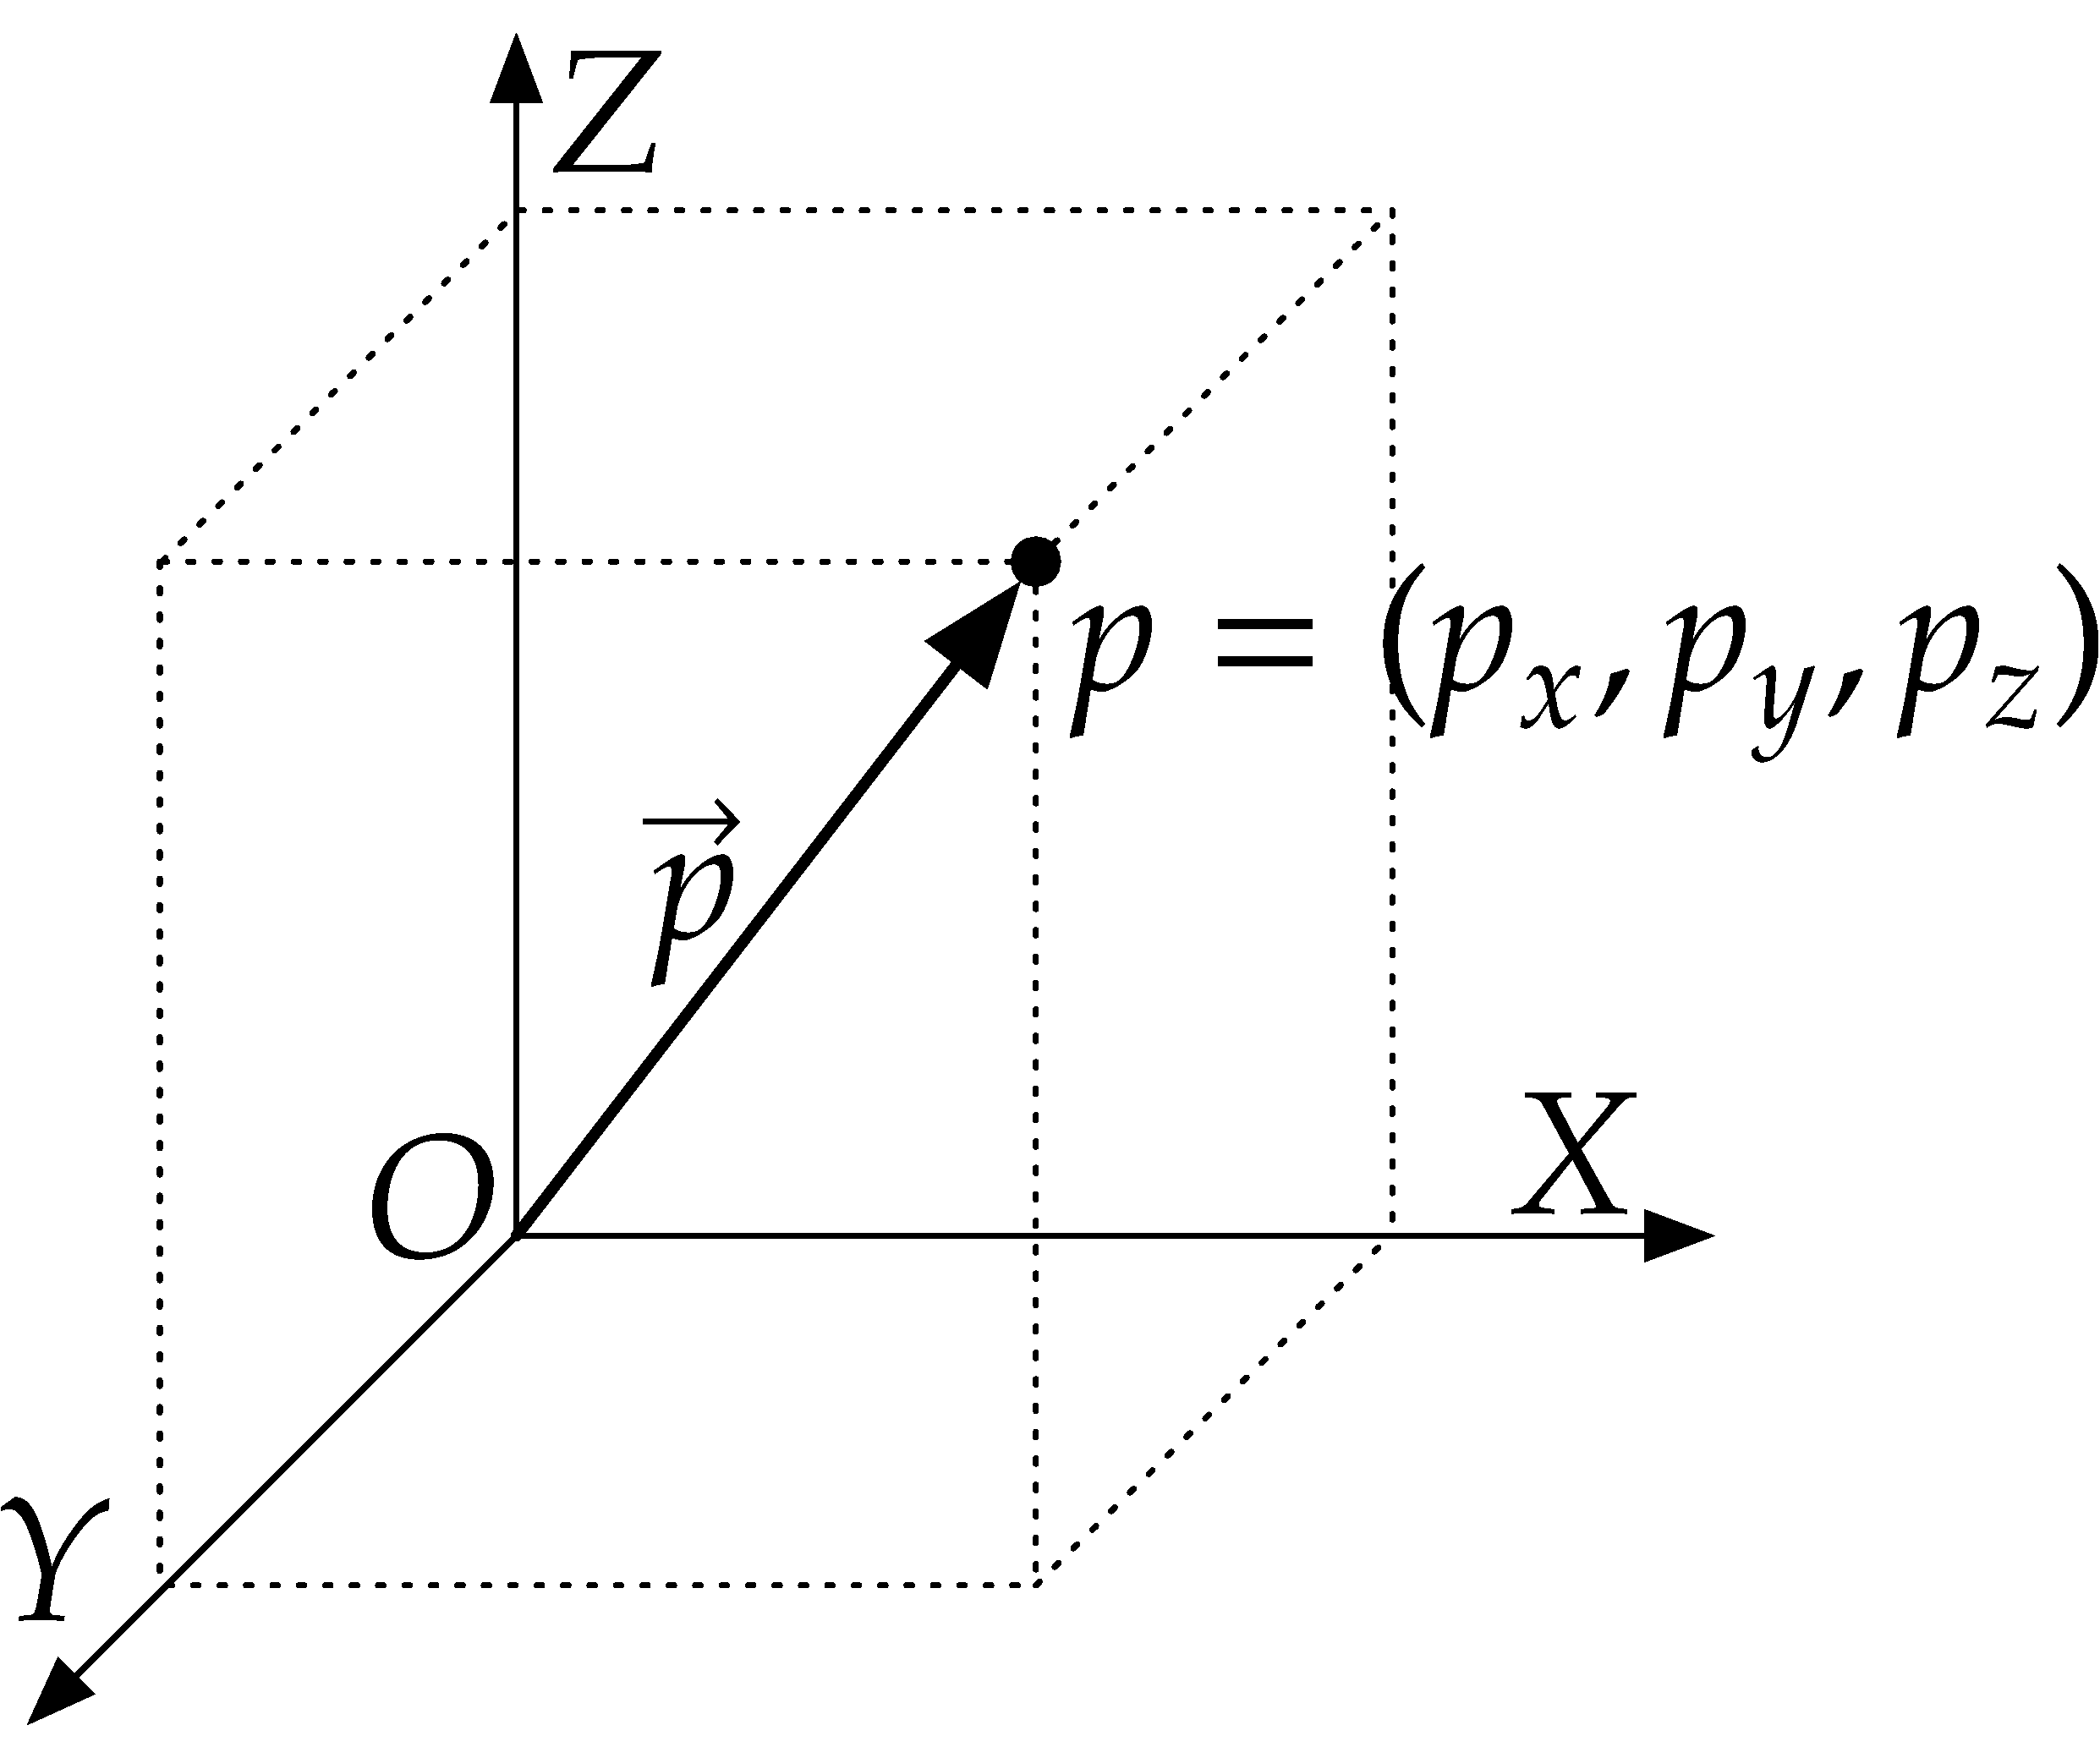
\includegraphics[width=\marginparwidth]{figs/point}
\caption{A point $p$ in 3D described by a treble $(p_x,p_y,p_z)$}
\label{fig:point}
}

A point $a = (a_1, a_2, \ldots, a_n)$ can also be used to define a vector $\vec{a}$, which goes from the origin to $a$.
% Why is            this vvvv necessary for spacing!?!?
The norm, or magnitude of\ \ $\vec{a}$, denoted as $\| \vec{a} \|$, gives the length of the line segment between $a$ and the origin and is computed as:
\begin{equation*}
\| \vec{a} \| = \sqrt{{a_1}^{2} + {a_2}^{2} + \cdots + {a_n}^{2}}
\end{equation*}

This analytic description of objects also enables using algebra to compute properties, such as the Euclidean distance between two points $a = (a_1, a_2, \ldots, a_n)$ and $b = (b_1, b_2, \ldots, b_n)$, also known as the Euclidean metric.
This is given by:
\begin{equation*}
\mathrm{distance}(a,b) = \sqrt{{(a_1 - b_1)}^{2} + {(a_2 - b_2)}^{2} + \cdots + {(a_n - b_n)}^{2}}
\end{equation*}

Some other objects can be described as a linear combination of linearly independent points (\ie\ two different points, three non-collinear points, four non-coplanar points, etc.).
Considering the points $p_1,p_2,\ldots,p_n$, a linear combination of them takes the form $a_1 p_1 + a_2 p_2 + \cdots + a_n p_n$, where $\sum_{i=1}^n a_i = 1$.
For every point $p_i$, $a_i$ is thus a scalar coefficient that determines its \emph{weight}.

If negative weights are allowed, the linear combination of $n+1$ linearly independent points forms an $n$-dimensional unbounded linear object, \eg\ a line using two points or a plane using three points.
All of these points lie exactly on the object.
When the weights are instead restricted to the interval $[0,1]$, the linear combination of $n+1$ linearly independent points forms an $n$-dimensional simplex (called an $n$-simplex)---a convex shape with $n+1$ vertices.
A \emph{0-simplex} is thus a point, a \emph{1-simplex} is a line segment, a \emph{2-simplex} is a triangle, a \emph{3-simplex} is a tetrahedron, and so on.

Other, more complex objects can be described using equations, which describe particular subsets of $\mathbb{R}^n$.
A hyperplane in $\mathbb{R}^n$, \ie\ a space of dimension $\mathbb{R}^{n-1}$ in $\mathbb{R}^n$, can be described by a linear equation of the form $a_1 x_1 + a_2 x_2 + \cdots + a_n x_n = b$, where $a_1, a_2, \ldots, a_n$ are the coefficients of the linear equation.
Apart from the points exactly on the hyperplane, as shown in \reffig{fig:halfspaces}, such a hyperplane separates $\mathbb{R}^n$ into two parts on either side of it.
\marginpar{
\captionsetup{type=figure}
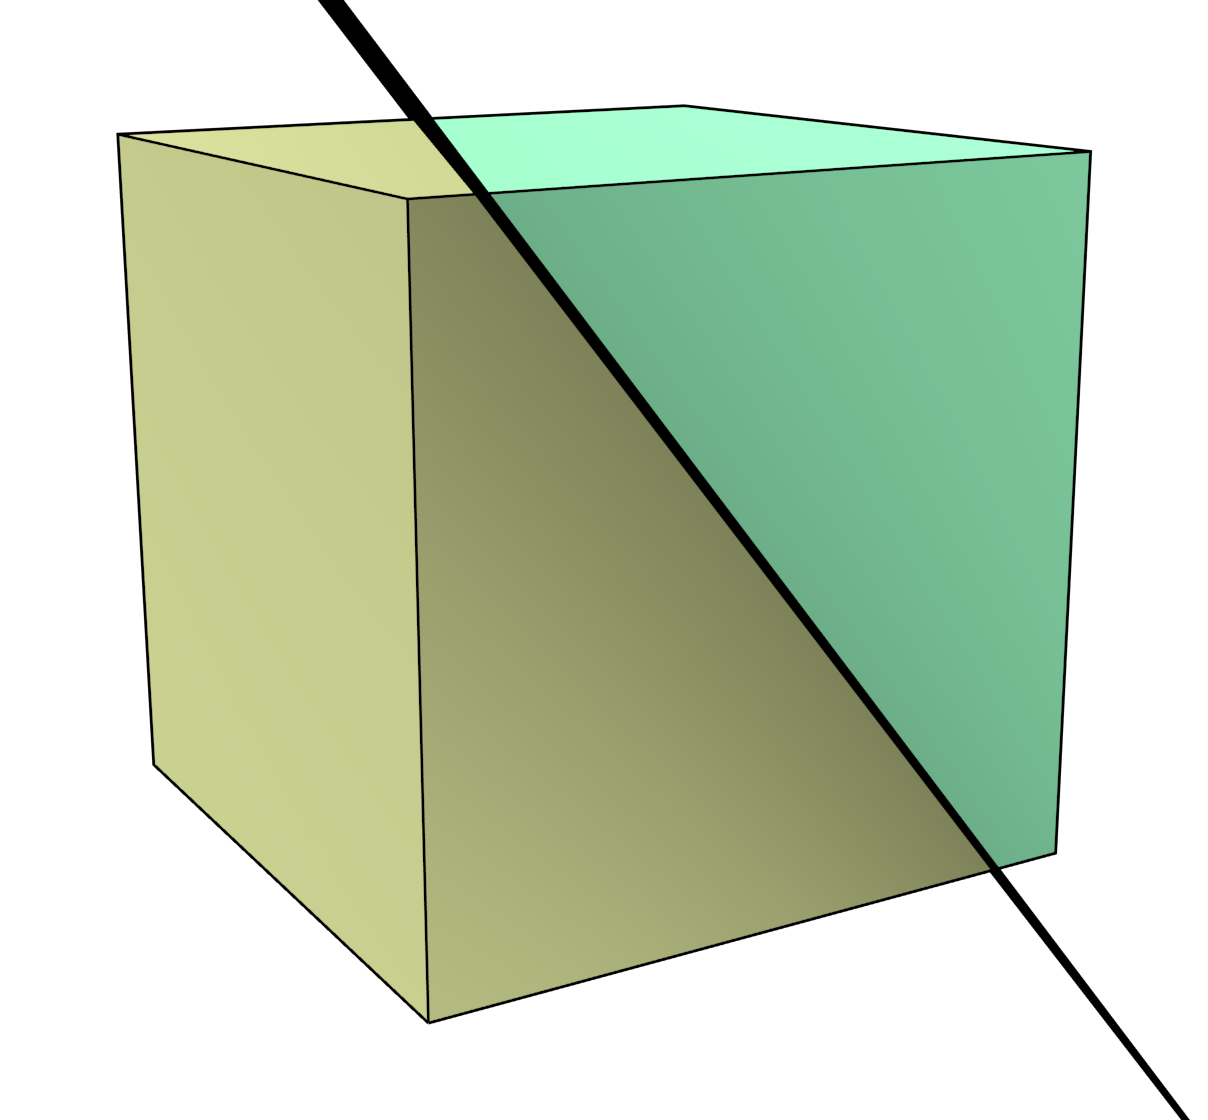
\includegraphics[width=\marginparwidth]{figs/halfspaces}
\caption{A plane separates $\mathbb{R}^3$ into two parts on either side of it.}
\label{fig:halfspaces}
}
These are known as open half-spaces and can be obtained by transforming the linear equation into the strict linear inequalities: $a_1 x_1 + a_2 x_2 + \cdots + a_n x_n < b$ for the half-space below the hyperplane and $a_1 x_1 + a_2 x_2 + \cdots + a_n x_n > b$ for the one above it.
If non-strict linear inequalities are used instead (\ie\ using $\leq$ and $\geq$ instead of $<$ and $>$), these \emph{closed half-spaces} also contain the points on the hyperplane.

Considering that a point can be described as a tuple of its coordinates, a hyperplane as a tuple of its coefficients, and similar constructions are possible for many other objects (\eg\ a sphere based on a centre point and radius), it becomes possible to have a \emph{computer representation} of these objects simply by storing tuples of numbers in a data structure\footnote{This hides the fact that using real numbers in a computer is very difficult in practice, thus floating-point approximations are generally used instead \citep{Goldberg91}.
The main consequences of this in spatial modelling are discussed in \refse{se:computerarithmetic}.}.
Moreover, it becomes possible to use them as a basis to describe other, more complex objects by using them as building blocks, either directly or using some of the topological concepts described in the next section, \eg\ them forming the boundary of another object.

Since analytic geometry allows the description of objects as sets of points in $\mathbb{R}^n$, as shown in \reffig{fig:boolean}, it is also possible to define objects based on Boolean set operations of their point sets.
\begin{figure}[hb]
\centering
\subfloat[$\mathbb{A}$ (purple) and $\mathbb{B}$ (blue)]{
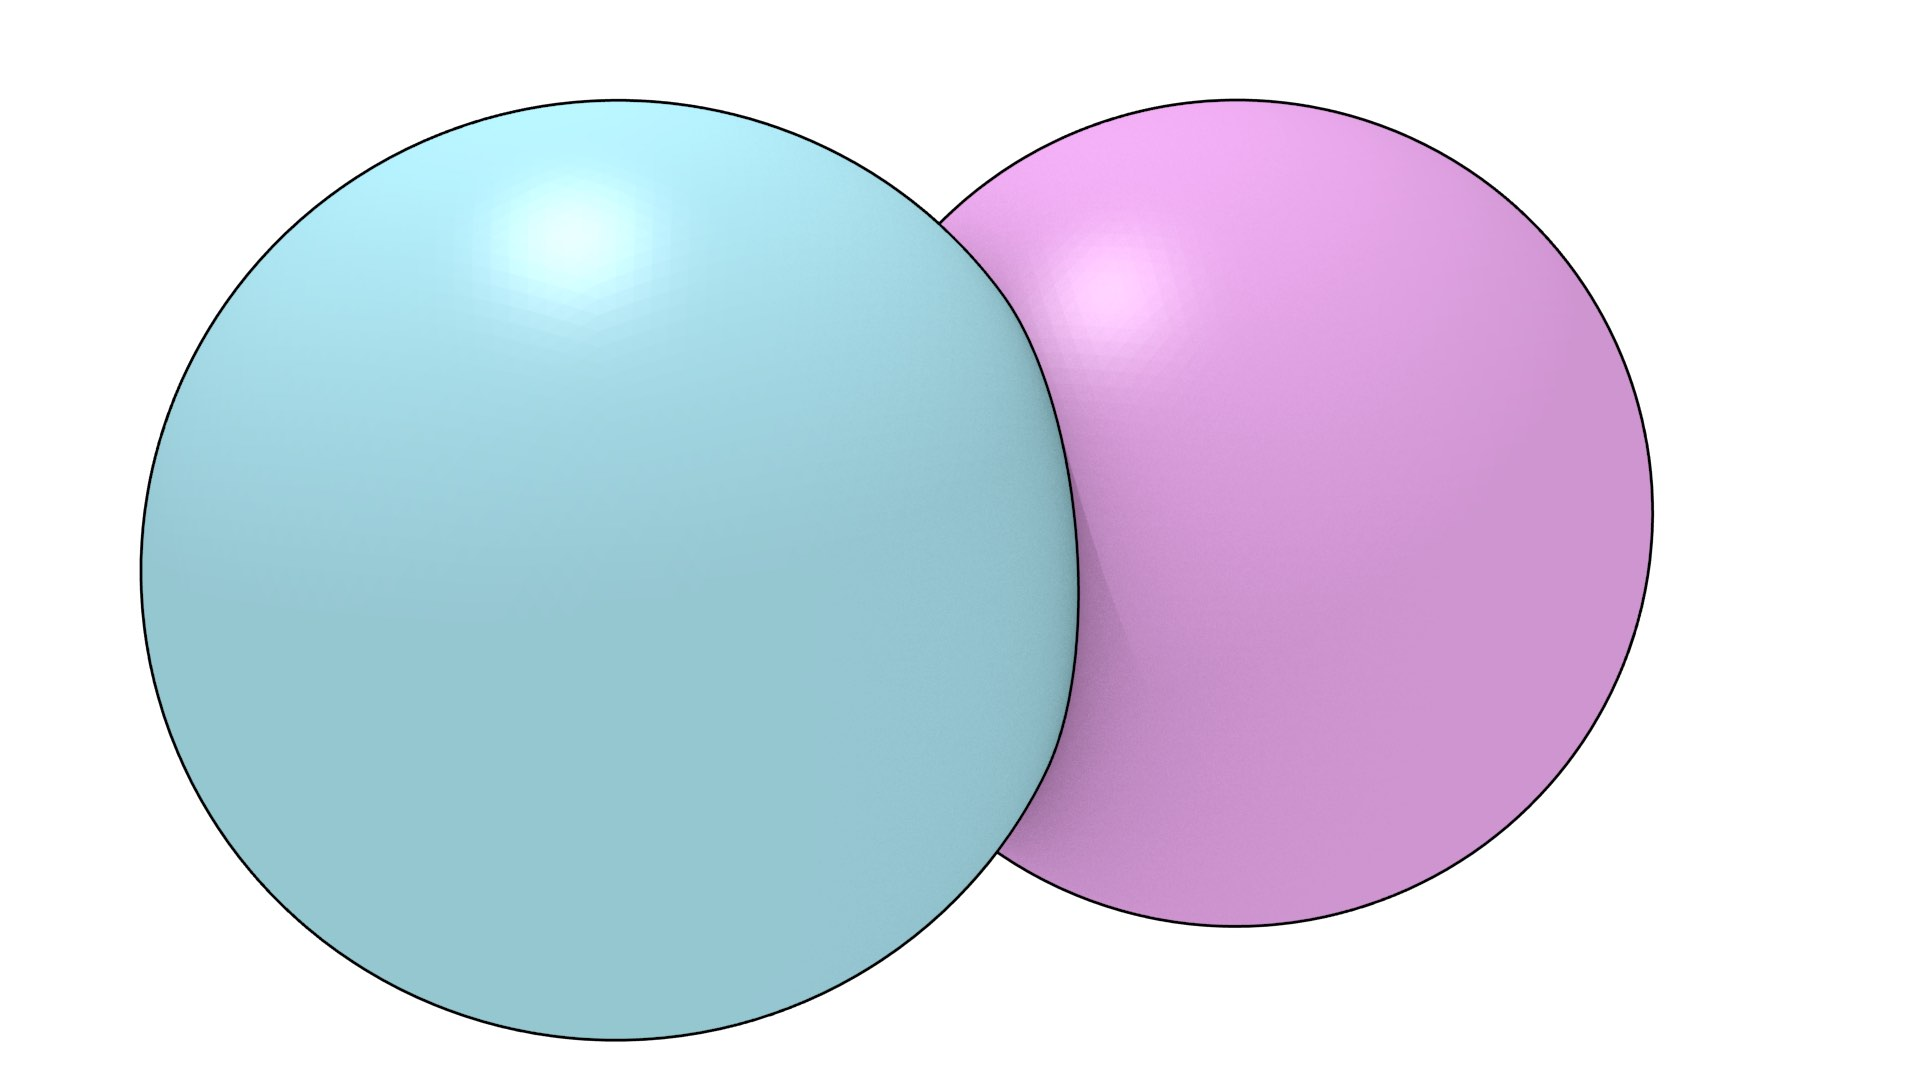
\includegraphics[width=0.5\linewidth]{figs/boolean}
\label{subfig:boolean}}
% \quad
\subfloat[Intersection: $\mathbb{A} \cap \mathbb{B}$]{
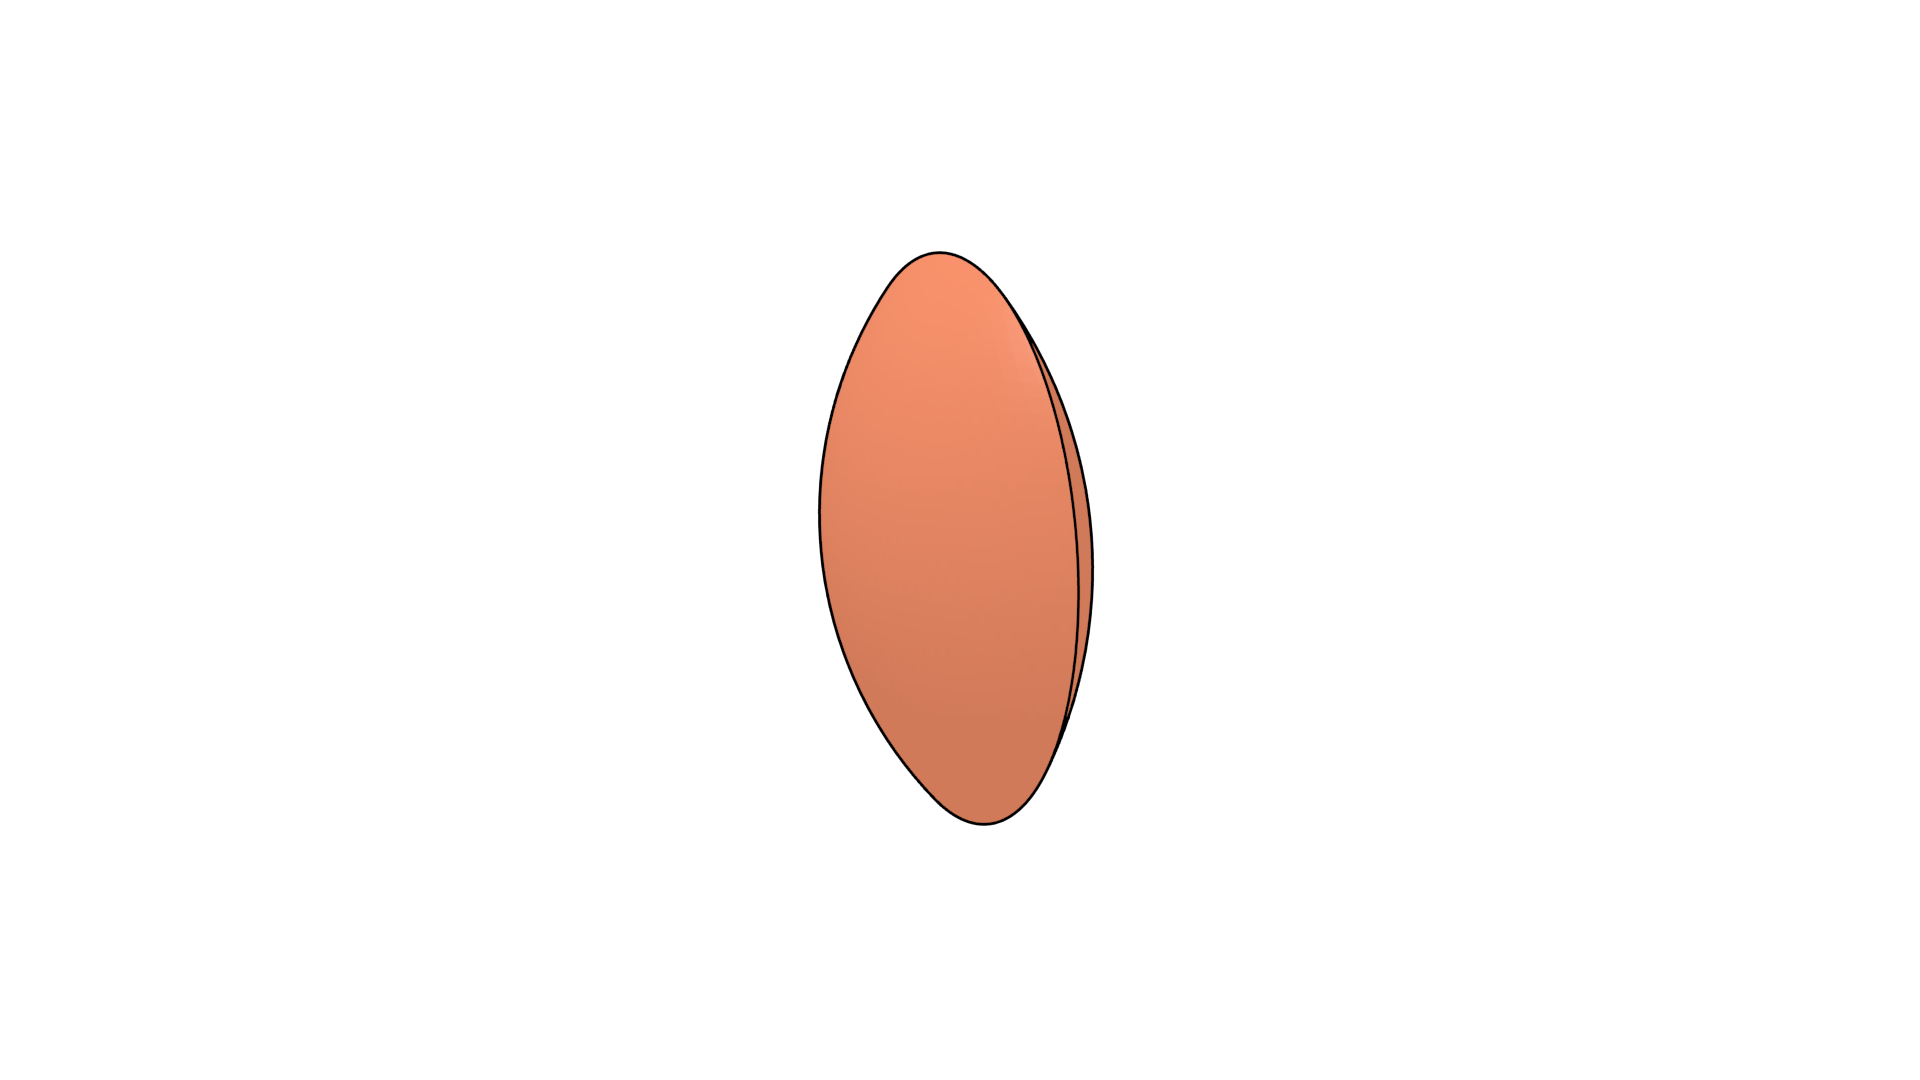
\includegraphics[width=0.5\linewidth]{figs/boolean-intersection}
\label{subfig:boolean-intersection}}
\\
\subfloat[Union: $\mathbb{A} \cup \mathbb{B}$]{
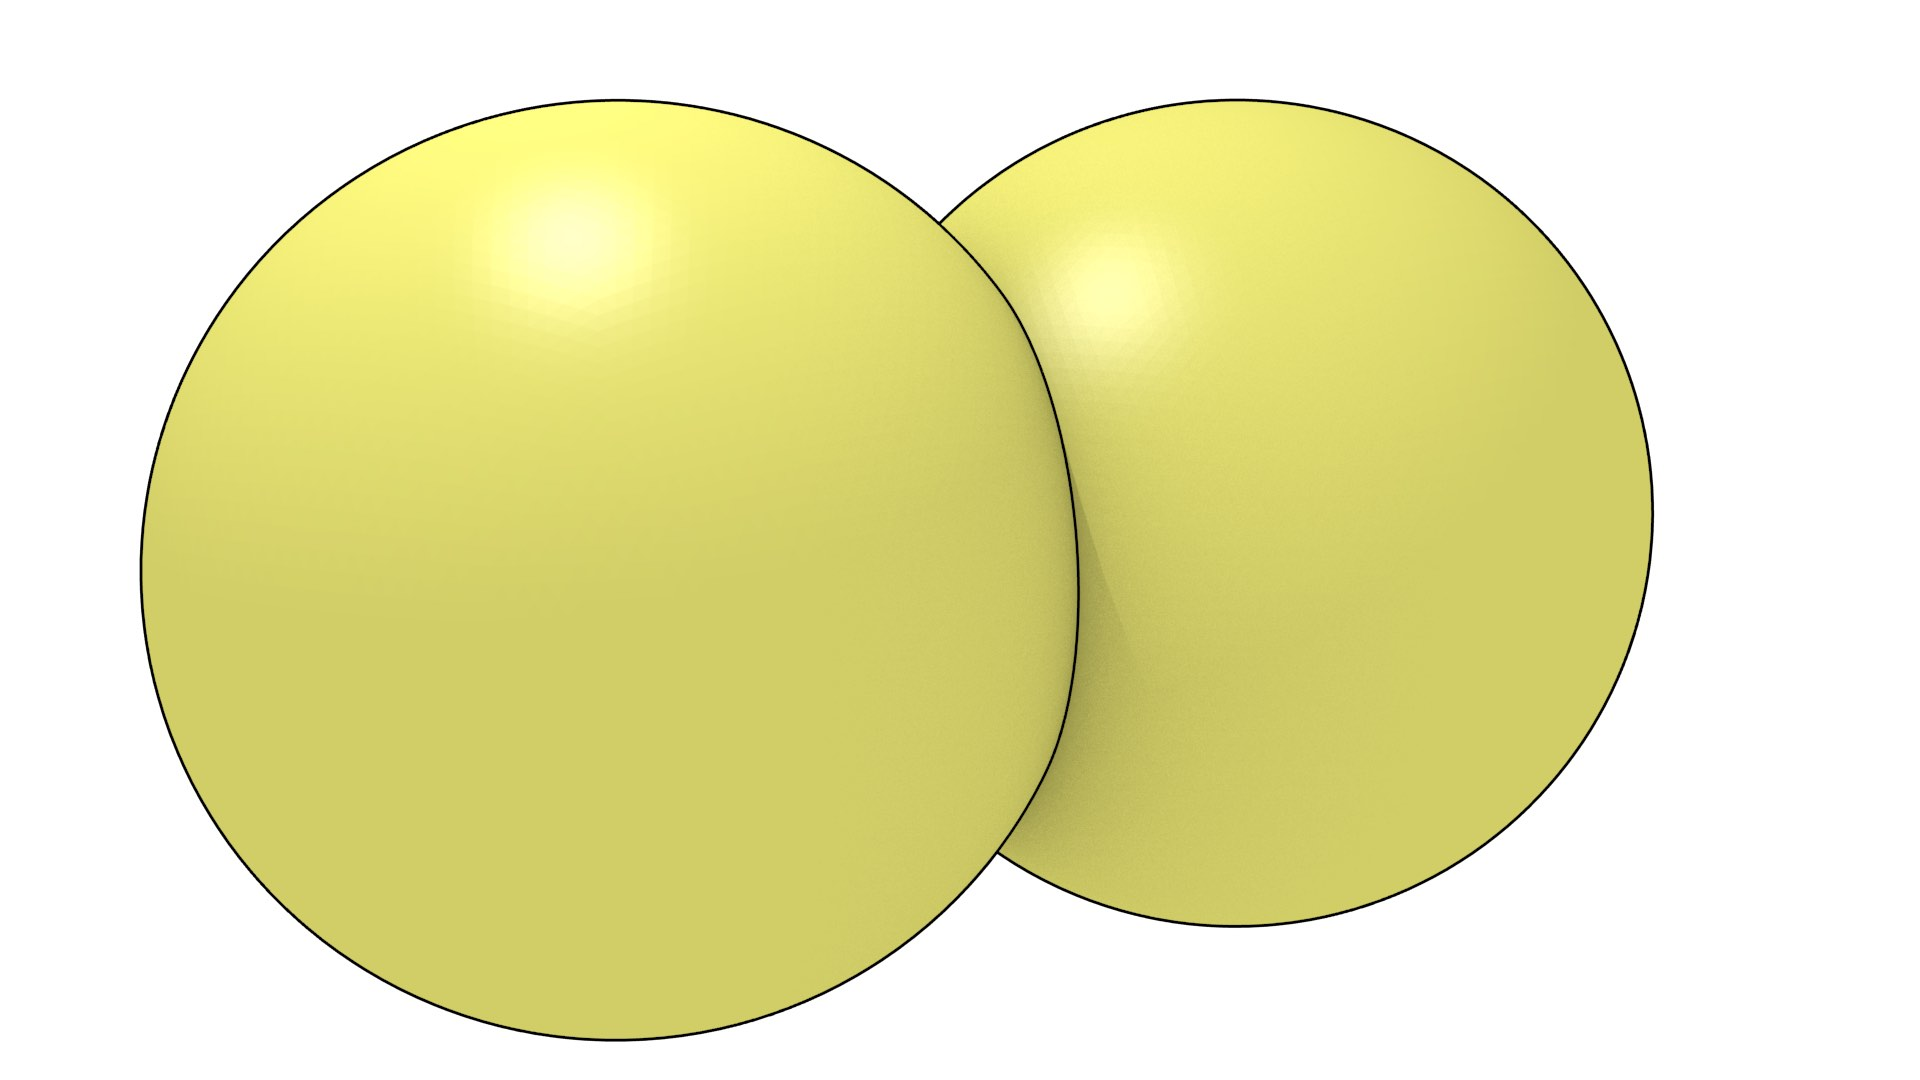
\includegraphics[width=0.5\linewidth]{figs/boolean-union}
\label{subfig:boolean-union}}
% \quad
\subfloat[Difference: $\mathbb{A} - \mathbb{B}$]{
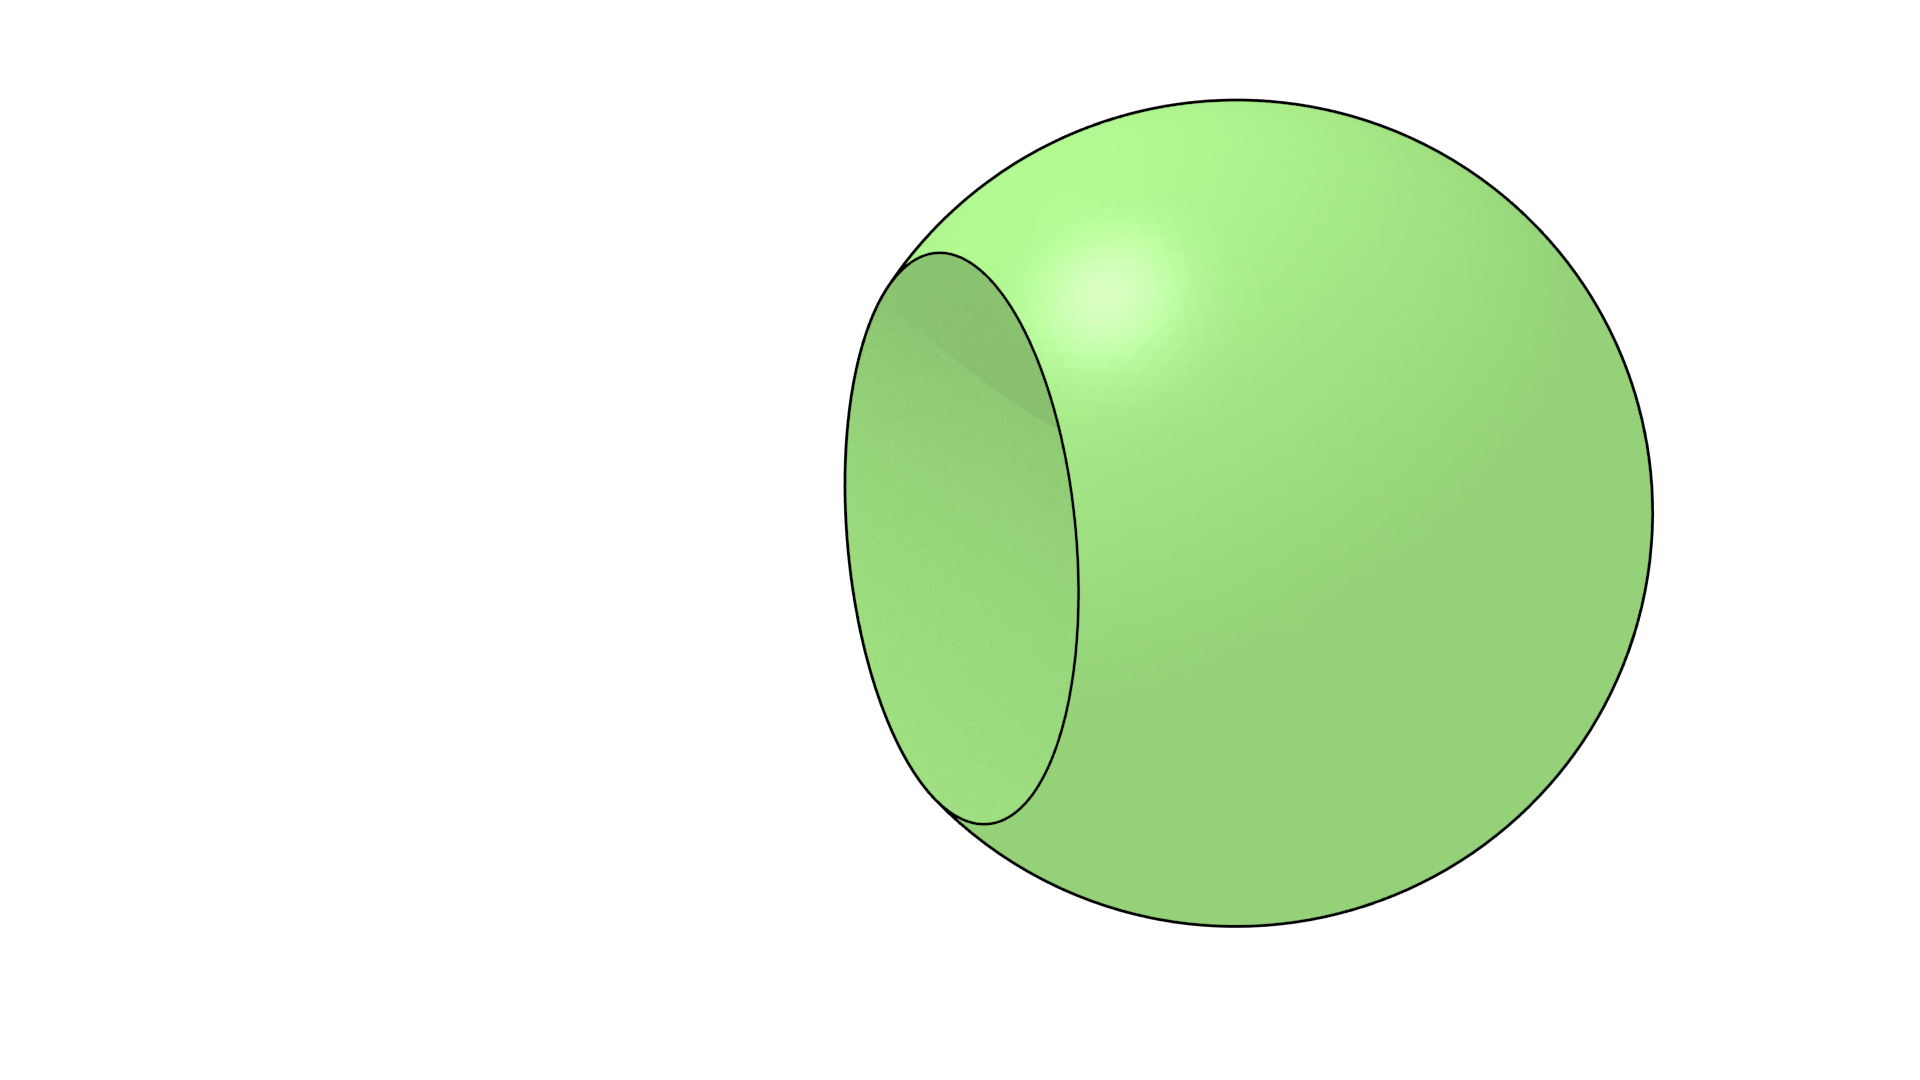
\includegraphics[width=0.5\linewidth]{figs/boolean-difference}
\label{subfig:boolean-difference}}
\caption[Objects can be defined using Boolean set operations]{Based on two balls $\mathbb{A}$ and $\mathbb{B}$, other objects that can be defined using Boolean set operations.}
\label{fig:boolean}
\end{figure}

\section{Topology}
\label{se:topology}

Topology is the mathematical study of the shape of objects, growing out of the analysis of certain problems in geometry, such as the boundaries of objects and the different possible notions of connectedness.
In particular, it studies the properties of certain objects that are preserved under so-called \emph{topological transformations} or \emph{continuous maps}, which include stretching and bending but exclude tearing or gluing.

There are two branches of topology that are most relevant in the context of spatial modelling, \emph{point-set topology} and \emph{algebraic topology}, respectively presented in \refse{ss:point-set-topology} and \refse{ss:algebraic-topology}.
Point-set topology describes space using concepts derived mainly from set theory, representing objects as continuous sets of points.
The properties of these sets and the relationships between multiple sets can then be analysed and described.
Algebraic topology adds concepts from abstract algebra as well, representing objects as structured sets of discrete elements, such as points, edges and faces.
As these elements and the relationships between them are both discrete, it is possible to use a wide variety of algorithmic methods on them, including graph theory, combinatorics, algorithmic algebra, and computational geometry and topology.

\subsection{Point-set topology}
\label{ss:point-set-topology}

Point-set topology, also known as general topology, describes objects as sets of points satisfying certain conditions, such as those in the construction in \reffig{fig:pointset}.
\marginpar{
\captionsetup{type=figure}
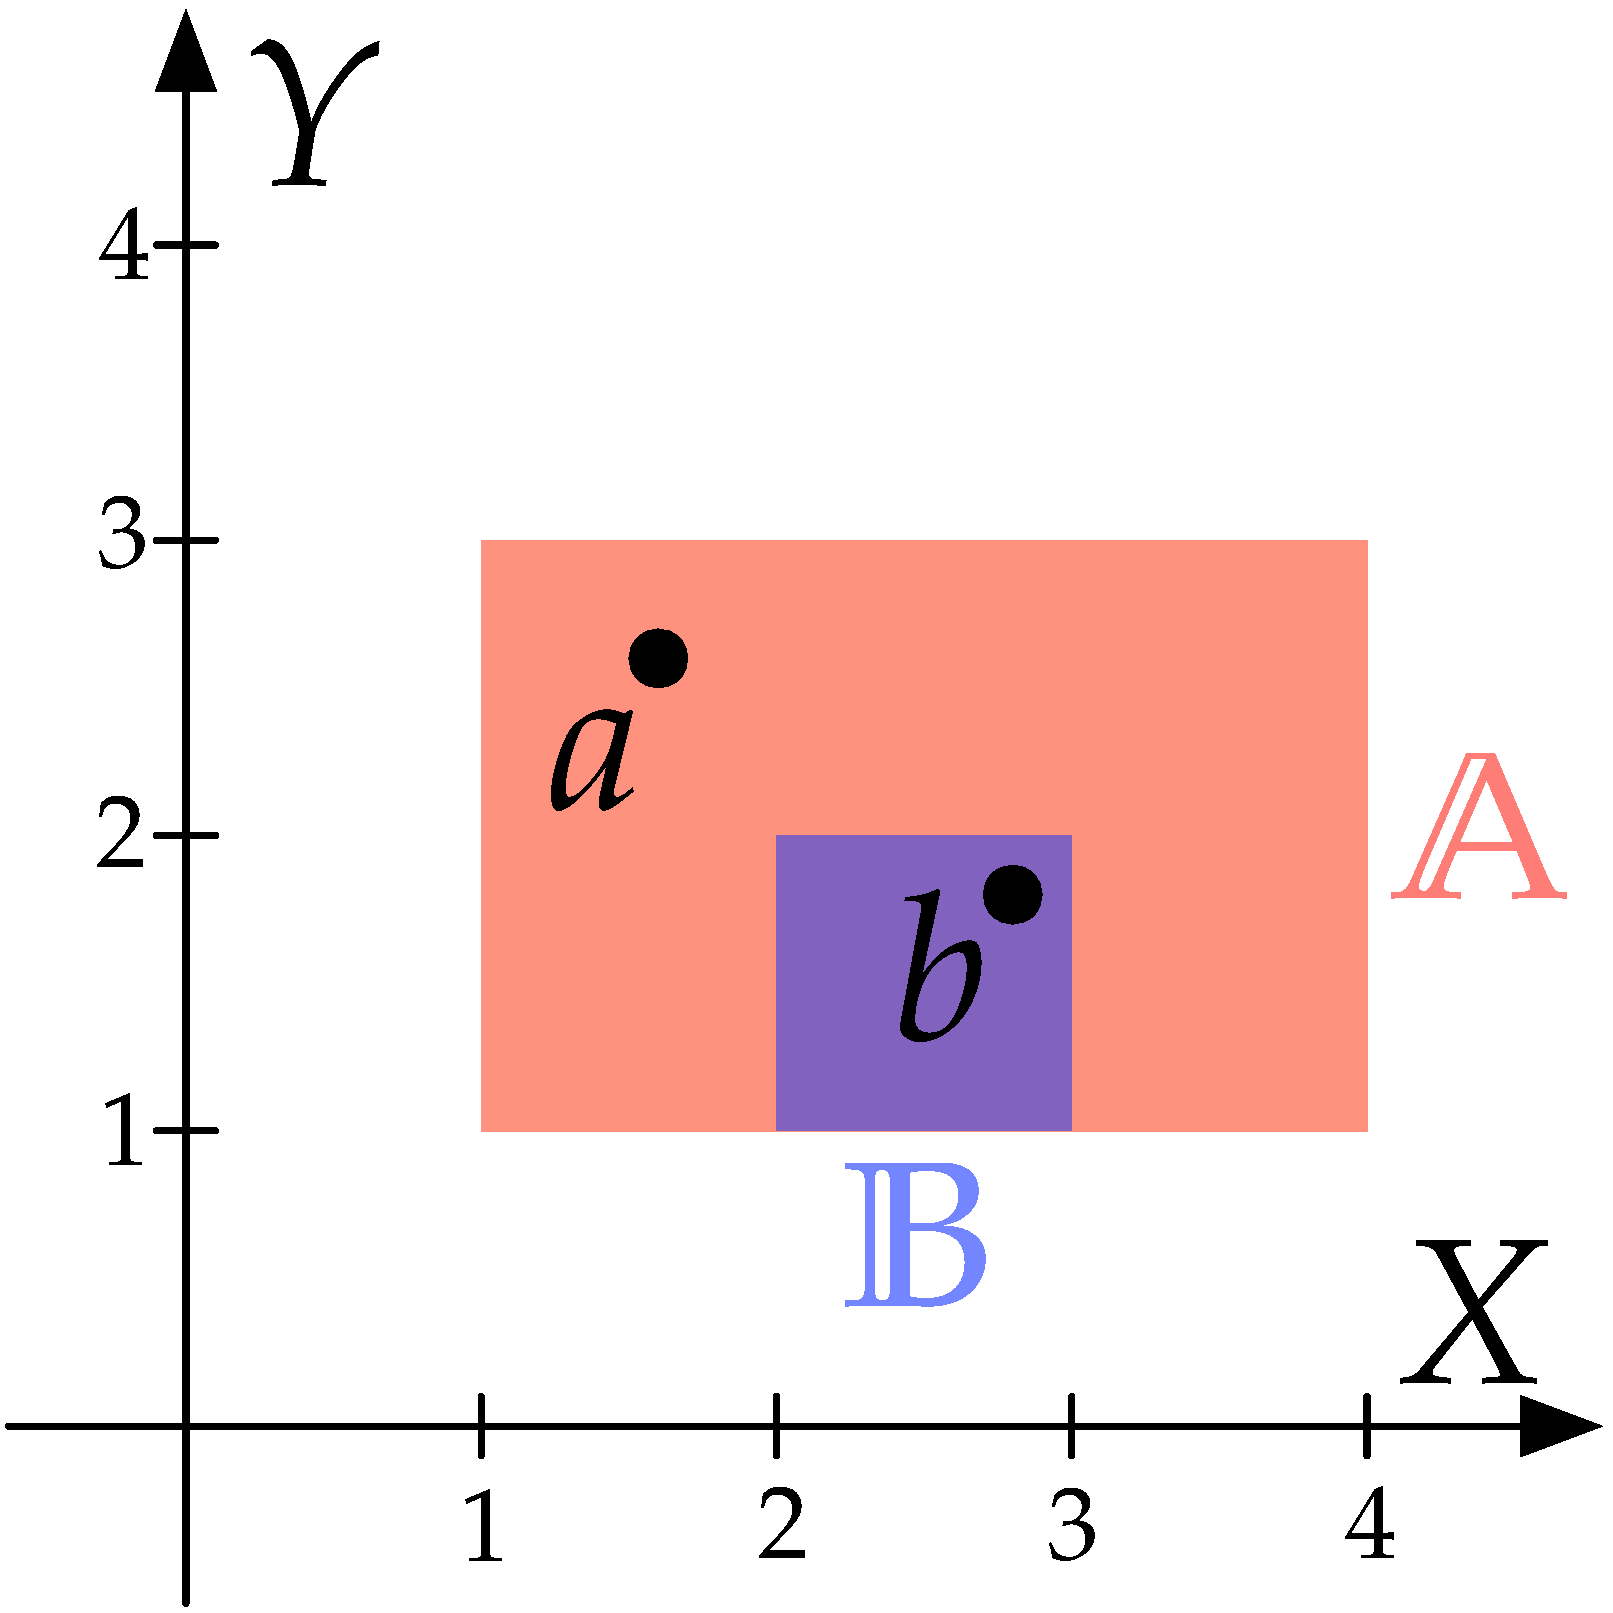
\includegraphics[width=\marginparwidth]{figs/pointset}
\caption[Two rectangles and two points defined as point sets]{The rectangle $\mathbb{A}$ is represented by the set of points where $1 \leq x \leq 4$ and $1 \leq y \leq 3$. In more compact (set builder) notation, $\mathbb{A} = \left\{ (x,y) \middle| x \in [1,4] \wedge y \in [1,3] \right\}$.
For the other objects, rectangle $\mathbb{B} = \left\{ (x,y) \middle| x \in [2,3] \wedge y \in [1,2] \right\}$, point $a \in \mathbb{A}$, point $b \in \mathbb{B}$ and point $b \in \mathbb{A}$.
$\mathbb{B}$ is a subset of $\mathbb{A}$ (\ie\ $\mathbb{B} \subset \mathbb{A}$).
}
\label{fig:pointset}
}
These objects can then be analysed based on the properties of the sets that describe them, such as whether a set is bounded or unbounded, has a certain number of holes, or is orientable or unorientable.
When multiple objects are present, the relationships between their corresponding sets can be analysed as well, such as whether they are touching or overlapping, or whether it is possible to define a function that maps between these sets.

Point-set topology works with \emph{topological spaces}, a much more general notion than that of Euclidean space.
This allows the description of different types of space with different properties.
A topological space consists of a set of points and a \emph{topology} on them satisfying a series of axioms.
\citet{Edelsbrunner14} provides the following simple formulation.
Given a set of points $\mathbb{X}$, a topology of $\mathbb{X}$ is a collection of subsets, which are called open sets\footnote{Note that there are alternative definitions based on the concepts of closed sets or of neighbourhoods \citep{Hausdorff14}. For a simple definition using neighbourhoods in a GIS context see \citet[\S{}3.2.2]{Worboys04}.}, such that:
\begin{itemize}
\item $\mathbb{X}$ is open and the empty set is open;
\item the intersection of any two open sets is open;
\item the union of any family of open sets is open.
\end{itemize}

While the definition of an open set for general topological spaces is rather complex, in the context of spatial modelling we are generally interested in Euclidean space, which has a straightforward definition analogous to the concept of an open interval in 1D (\reffig{fig:intervals}).
\marginpar{
\captionsetup{type=figure}
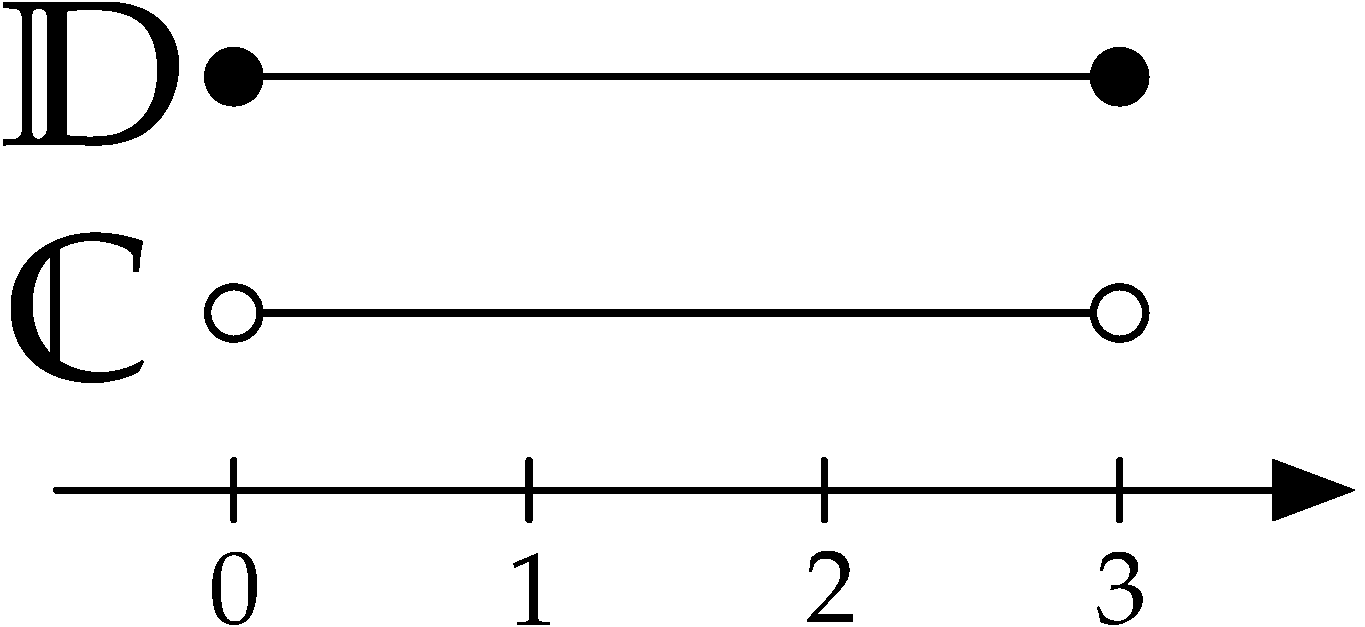
\includegraphics[width=\marginparwidth]{figs/intervals}
\caption[Open and closed intervals]{An open interval $\mathbb{C} = (0,3) = \left\{x \middle| 0 < x < 3 \right\}$ does not include its endpoints. By contrast, a closed interval $\mathbb{D} = [0,3] = \left\{x \middle| 0 \leq x \leq 3 \right\}$ includes its endpoints.}
\label{fig:intervals}
}
A point set $\mathbb{S}$ in Euclidean space is open if, given any point $p \in \mathbb{S}$, there exists a real number $\epsilon > 0$ such that, given any point $q$ whose Euclidean distance to $p$ is smaller than $\epsilon$, then $q \in \mathbb{S}$ as well.
A point set is closed when the point set formed by its complement is open.
Any point on an open interval fulfils these conditions, but the endpoints of a closed interval do not.
Note that it is possible for a set to be open \emph{and} closed (\eg\ an interval containing only one of its endpoints).

For example, in 2D, the plane together with the topology generated by the Euclidean metric is the topological space known as the \emph{Euclidean topology of the plane}, which can be defined based on \emph{open disks}, which are analogous to 1D open intervals.
An open disk is the set of points closer to a point $p \in \mathbb{R}^2$ than a non-zero distance $r$, such as the unit open disk shown in \reffig{fig:unitopendisk}.
\marginpar{
\captionsetup{type=figure}
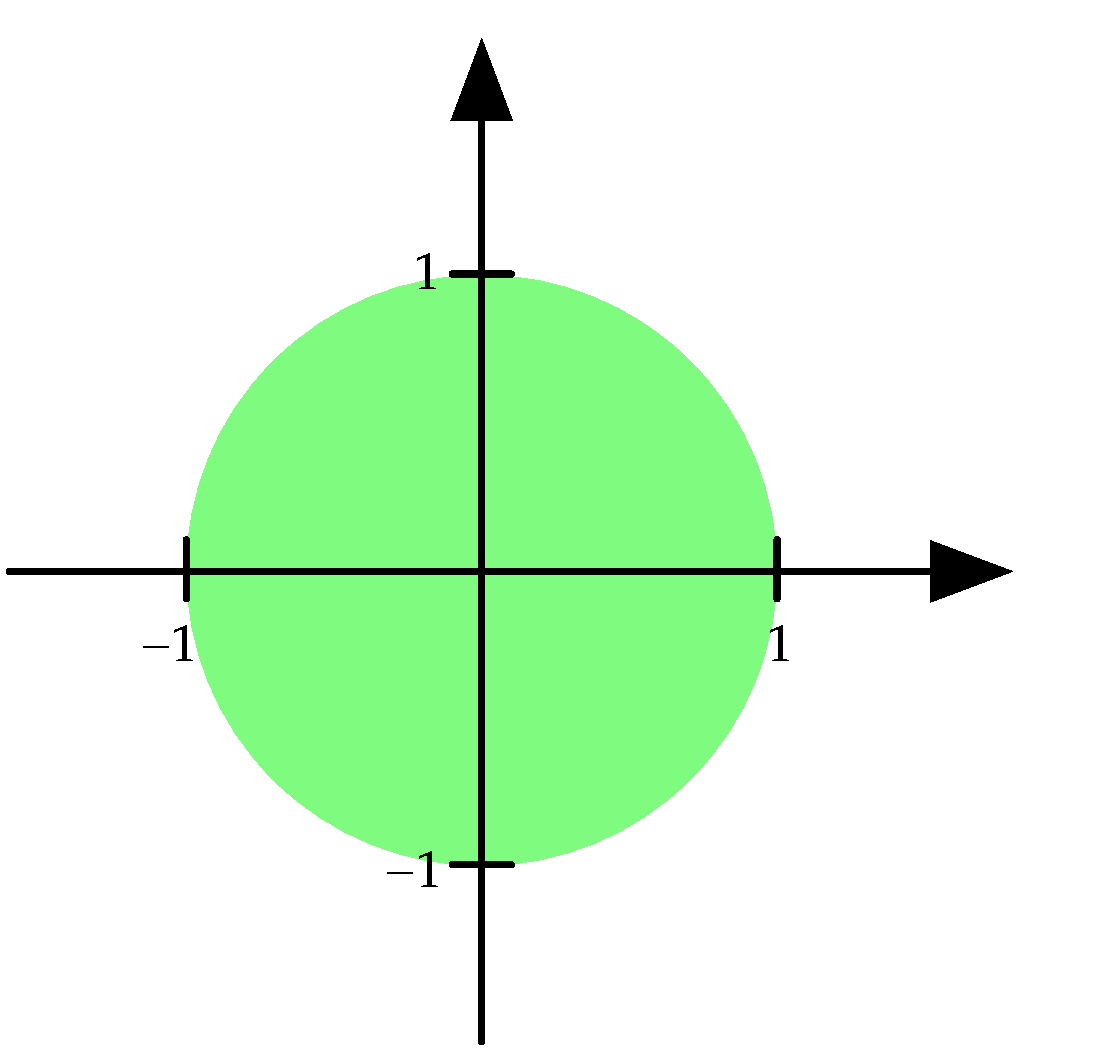
\includegraphics[width=\marginparwidth]{figs/unitopendisk}
\caption[The unit open disk]{The unit open disk, \ie\ an open disk of radius 1 centred at the origin can be defined as $\mathbb{D} = \left\{ x \in \mathbb{R}^2 \middle| \| x \| < 1 \right\}$.}
\label{fig:unitopendisk}
}
It is easy to see that as these 2D disks do not contain their boundaries, the intersection of any two open disks and the union of any number of disks are both open.

Based on the concepts of open intervals in 1D, open disks in 2D, or open balls when talking about any dimension, it is possible to partition a Euclidean space into three parts: its \emph{interior}, \emph{boundary} and \emph{exterior}.
An example of these is shown in \reffig{fig:annulus}.
\marginpar{
\captionsetup{type=figure}
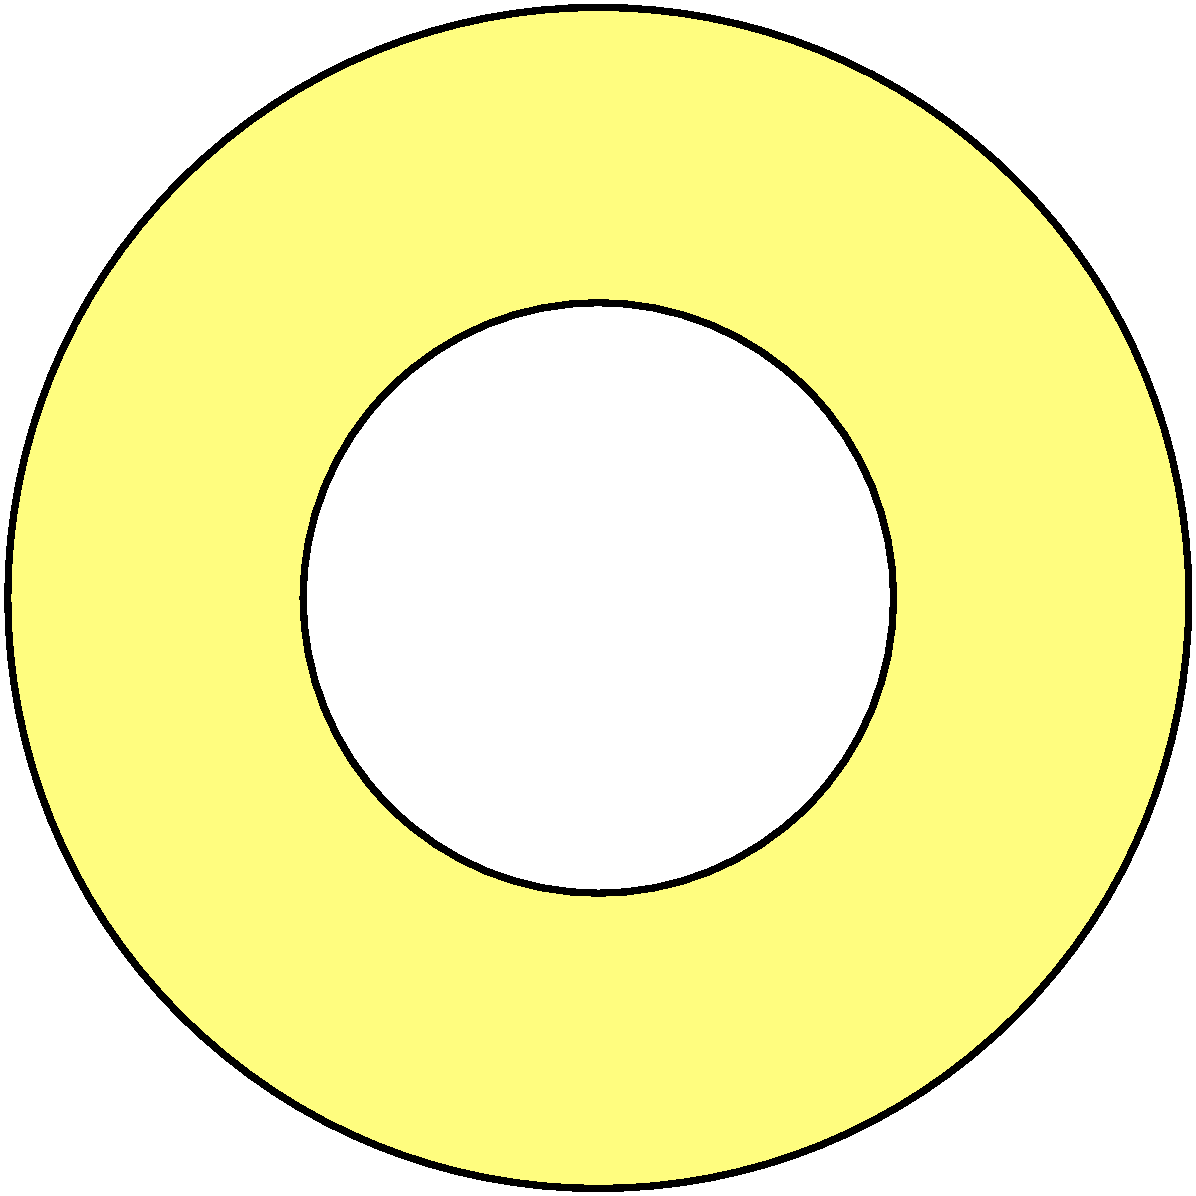
\includegraphics[width=\marginparwidth]{figs/annulus}
\caption[An annulus partitions the Euclidean plane into three parts]{An annulus with boundary partitions the Euclidean plane into three parts: its interior (yellow), its boundary (black) and its exterior (the rest of this page).
Note that none of these necessarily have to be connected.}
\label{fig:annulus}
}
The \emph{interior} of a point set $\mathbb{S}$ consists of all points where there exists an open ball centred at them such that all the points in the ball are in $\mathbb{S}$, the boundary of $\mathbb{S}$ consists of the points where all possible open balls centred at them have points in $\mathbb{S}$ and out of $\mathbb{S}$, and the exterior of $\mathbb{S}$ consists of all points where there exists an open ball centred at them such that all the points in the ball are out of $\mathbb{S}$.
The \emph{closure} of $\mathbb{S}$ is the union of its interior and its boundary.
The \emph{regularisation} of $\mathbb{S}$ is the closure of its interior and a point set is thus \emph{regular} when it is equal to its regularisation.

Once objects are defined as sets of points, point-set topology works with functions that relate these sets to each other.
A function from one point set to another is said to be \emph{continuous} if the preimage (\ie\ the inverse image) of every open set is open.
If a function is continuous and its inverse function is also continuous, it is known as a \emph{homeomorphism}.
When such a function exists between two point sets, they are said to be \emph{homeomorphic} or, more informally, \emph{topologically equivalent}, such as the two objects shown in \reffig{fig:homeomorphism}.

\begin{figure}[b]
\centering
\subfloat[A coffee mug]{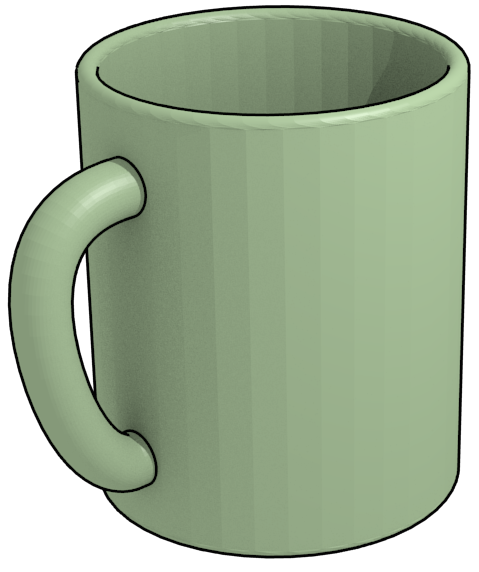
\includegraphics[width=\marginparwidth]{figs/mug}} \quad
\subfloat[A donut]{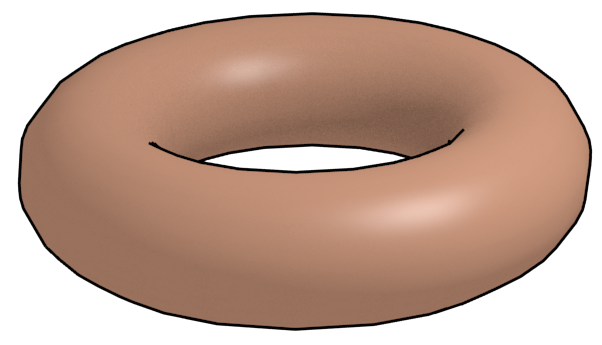
\includegraphics[width=\marginparwidth]{figs/donut}}
\caption[A coffee mug and a donut are homeomorphic]{A coffee mug and a donut are homeomorphic\footnotemark. Intuitively, this can be known as it is possible to deform one into the other. The mug was rendered from the model at \url{http://www.thingiverse.com/thing:7953}.}
\label{fig:homeomorphism}
\end{figure}
\footnotetext{Related to the joke: `A topologist is a mathematician who can't tell the difference between a coffee mug and a donut'.}

\begin{figure*}[tbp]
\centering
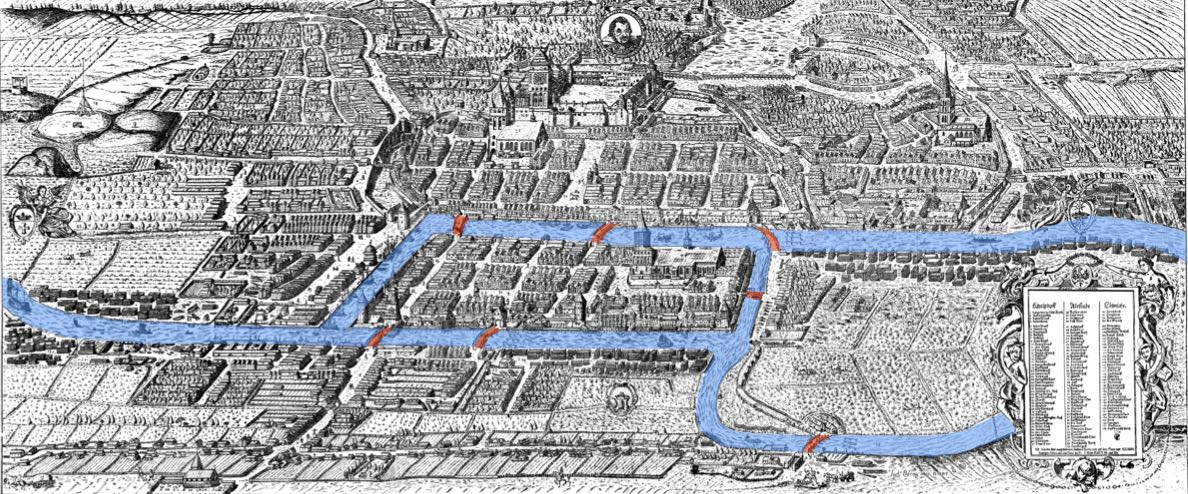
\includegraphics[width=\linewidth]{figs/konigsberg}
\caption[The Seven Bridges of K\"onigsberg]{The problem of the Seven Bridges of K\"onigsberg asks whether it is possible to find a route through the city that would cross each bridge (highlighted in red) exactly once. \citet{Euler41} proved that there is no such route in terms of a graph. Whenever one enters a piece of land by a bridge, one has to leave it by another bridge except at the beginning or end of the route. Thus, there must be an \emph{even} number of bridges connected to all but (at most) two pieces of land. Since all pieces of land have an \emph{odd} number of bridges, the problem has no solution. Based on an image from a 1613 engraving by Joachim Bering.}
\label{fig:konigsberg}
\end{figure*}

Another important topological concept is that of a manifold.
A manifold is a topological space that is homeomorphic to the Euclidean space of a certain dimension.
Intuitively, this means that a manifold locally resembles Euclidean space, even if globally it does not.
For example, a line and a circle are 1-manifolds, while a plane, a sphere and a torus are 2-manifolds.
Generally, when the term manifold is used in GIS it refers to a 2-manifold.

\subsection{Algebraic topology}
\label{ss:algebraic-topology}

Conceptually based on point-set topology, \emph{algebraic topology}, also known as combinatorial topology, uses concepts from abstract algebra in order to analyse topological spaces.
A famous early application involved the answer to the problem of the Seven Bridges of K\"onigsberg by \citet{Euler41}, explained in \reffig{fig:konigsberg}.
However, the real foundations of the field were set when many of its concepts were formalised in algebraic form by \citet{Poincare95}.

Algebraic topology works by relating topological spaces to groups with specific properties, often by creating combinatorial analogues of such spaces, from which their properties can be extracted using algebraic methods \citep{Henle94}, which can be applied algorithmically.
As it uses discrete structures rather than continuous point sets, it is often more suited to computer implementations of topological concepts than point-set topology \citep[\S{}3.3.5]{Worboys04}.

Two constructions of algebraic topology are widely used as the basis of GIS:\ \emph{simplicial complexes} and \emph{cell complexes}.
An $n$-dimensional simplicial complex is a structure made of connected \emph{simplices}, the simplest objects that can be built in any dimension.
As shown in \reffig{fig:simplex}, an $n$-dimensional simplex ($n$-simplex) is a combinatorial primitive made from a set of $n+1$ vertices.
\marginpar{
\captionsetup{type=figure}
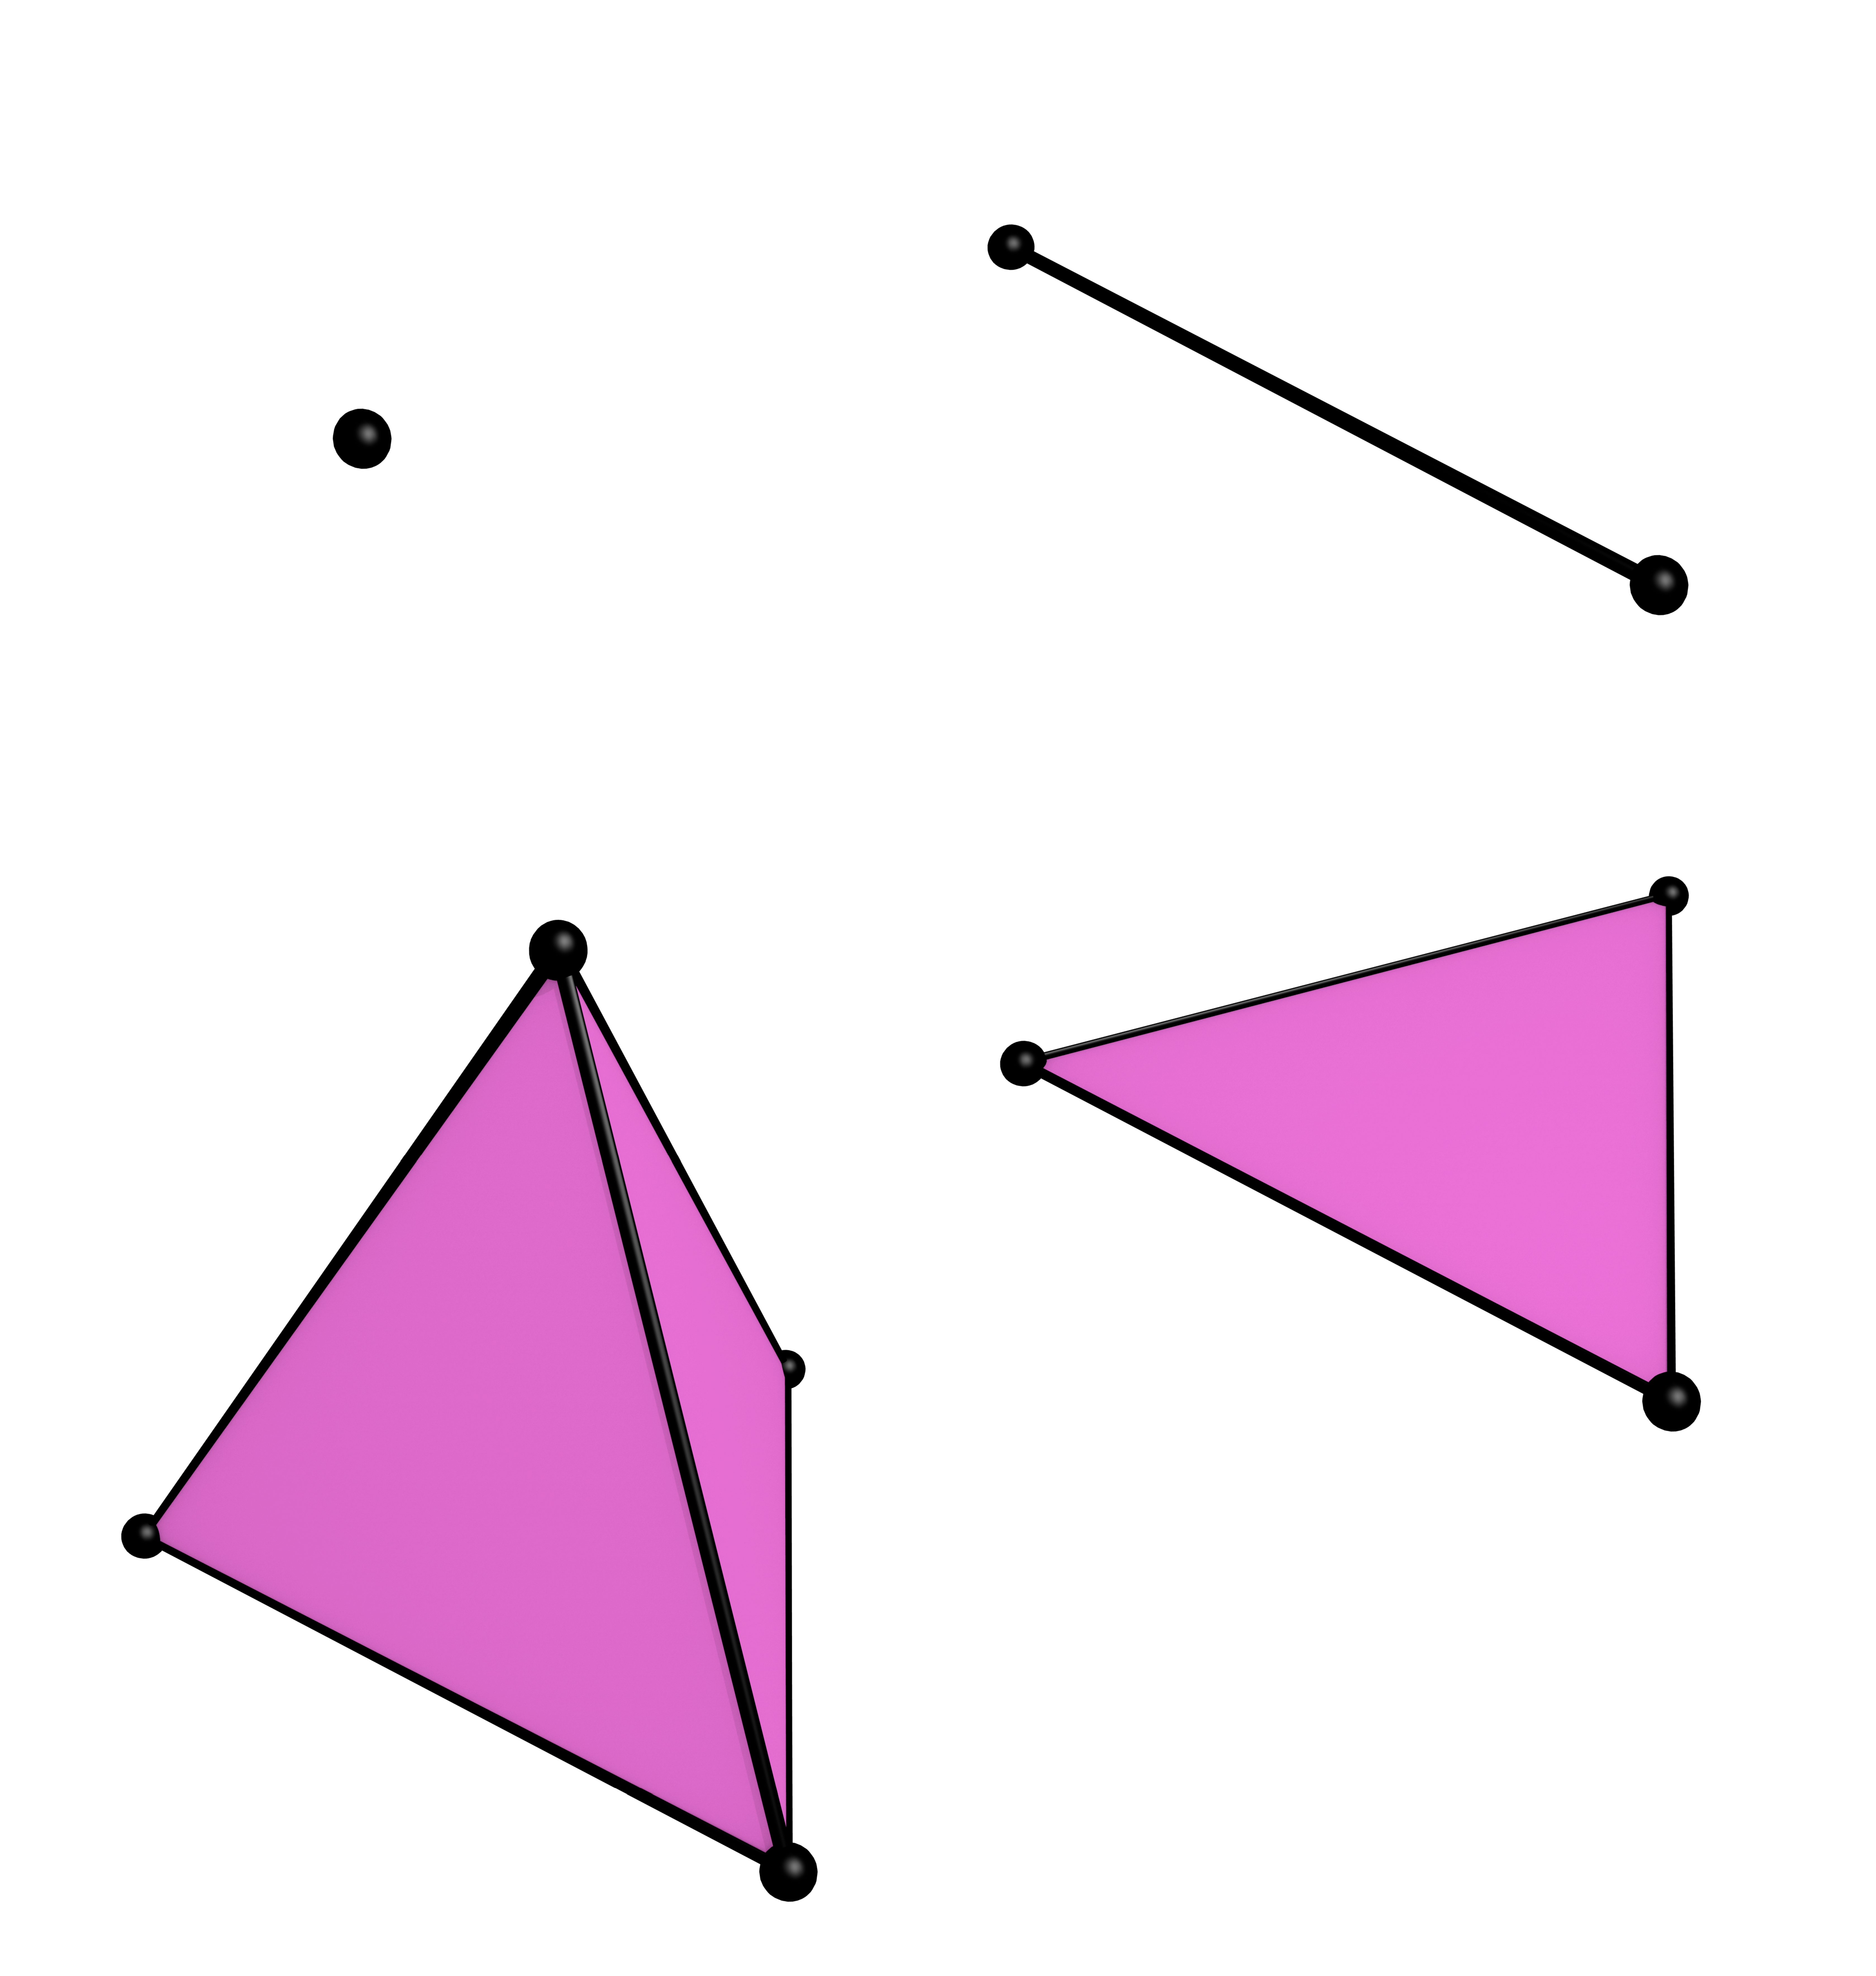
\includegraphics[width=\marginparwidth]{figs/simplex}
\caption[0-, 1-, 2- and 3-simplices]{An $n$-dimensional simplex is a combinatorial primitive made from a set of $n+1$ vertices. A 0-simplex is thus a point, a 1-simplex is a line segment, a 2-simplex is a triangle, and a 3-simplex is a tetrahedron. Here they are shown as if embedded in $\mathbb{R}^3$.}
\label{fig:simplex}
}
\reffig{fig:simplicescampus} shows a group of buildings represented as a 3D simplicial complex.
\begin{figure*}[b]
\centering
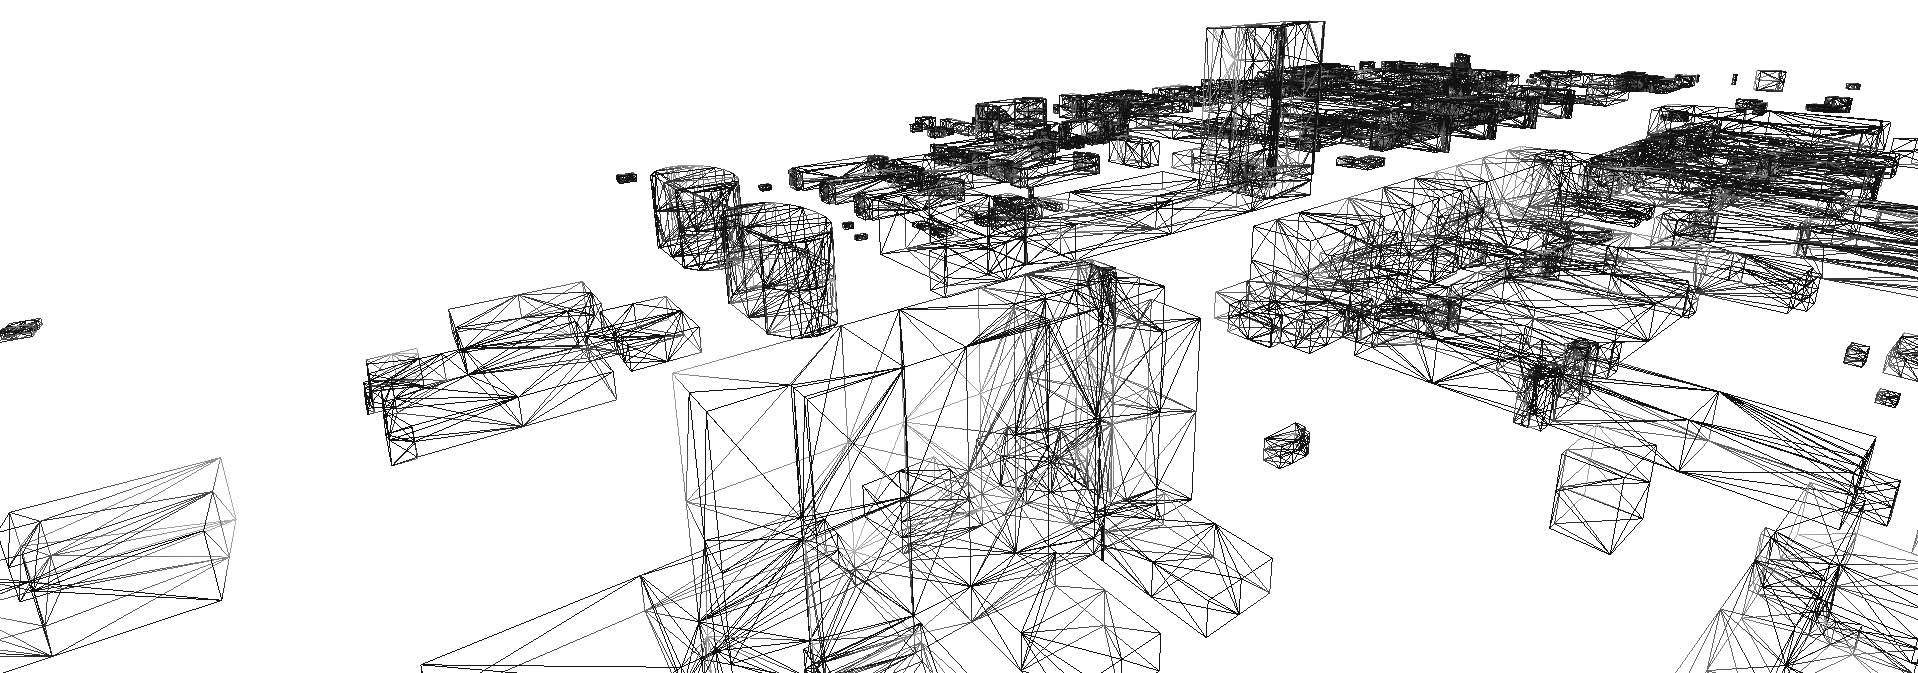
\includegraphics[width=\linewidth]{figs/simplicescampus}
\caption[The TU Delft campus as a 3D simplicial complex]{The buildings in the TU Delft campus are represented as a 3D simplicial complex, such that each separate building is a set of adjacent tetrahedra. Note that only the tetrahedra's edges are shown here.}
\label{fig:simplicescampus}
\end{figure*}
A 0D simplicial complex consists of a set of discrete points (\ie\ a point cloud) and a 1D simplicial complex is a plane graph.
A 2D simplicial complex is known as a \emph{triangulation} and a 3D simplicial complex as a \emph{tetrahedralisation}.

A $j$-dimensional face ($j$-face) of an $i$-simplex, $j < i$, is a $j$-simplex made from a proper subset of its vertices.
Sometimes the dimension of the face is omitted and it can be deduced from the context, but in GIS it generally refers to each of the $i+1$ $(i-1)$-faces of an $i$-simplex.
In the context of an $i$-dimensional simplicial complex, a face refers to each of the $i$-simplices in the complex, such as the triangles in a triangular mesh.

More formally, a simplicial complex can be defined as a collection of simplices such that:
\begin{itemize}
\item
every face of a simplex is also in the simplicial complex;
\item
the intersection of any two simplices is either empty or is a common face of both of them\footnote{Note that this implies a definition where a simplex contains its boundary.}.
\end{itemize}

Based on the set of common vertices shared by two simplices, it is possible to define certain \emph{topological relationships} between them.
Two $i$-simplices are said to be adjacent if they have a common $(i-1)$-face.
An $i$-simplex and a $j$-simplex, $i \neq j$, are said to be incident if either is a face of the other.

A cell complex is a structure made of connected \emph{cells}, where an $i$-dimensional cell ($i$-cell) is an object homeomorphic to an open $i$-ball (\ie\ point, open arc, open disk and open ball).
0-cells are known as vertices, 1-cells as edges, 2-cells as faces and 3-cells as volumes.
Considering only linear geometries, 1-cells are thus line segments, 2-cells polygons and 3-cells polyhedra.
\reffig{fig:cellscampus} shows a group of buildings represented as a 3D cell complex.
\begin{figure*}[tbp]
\centering
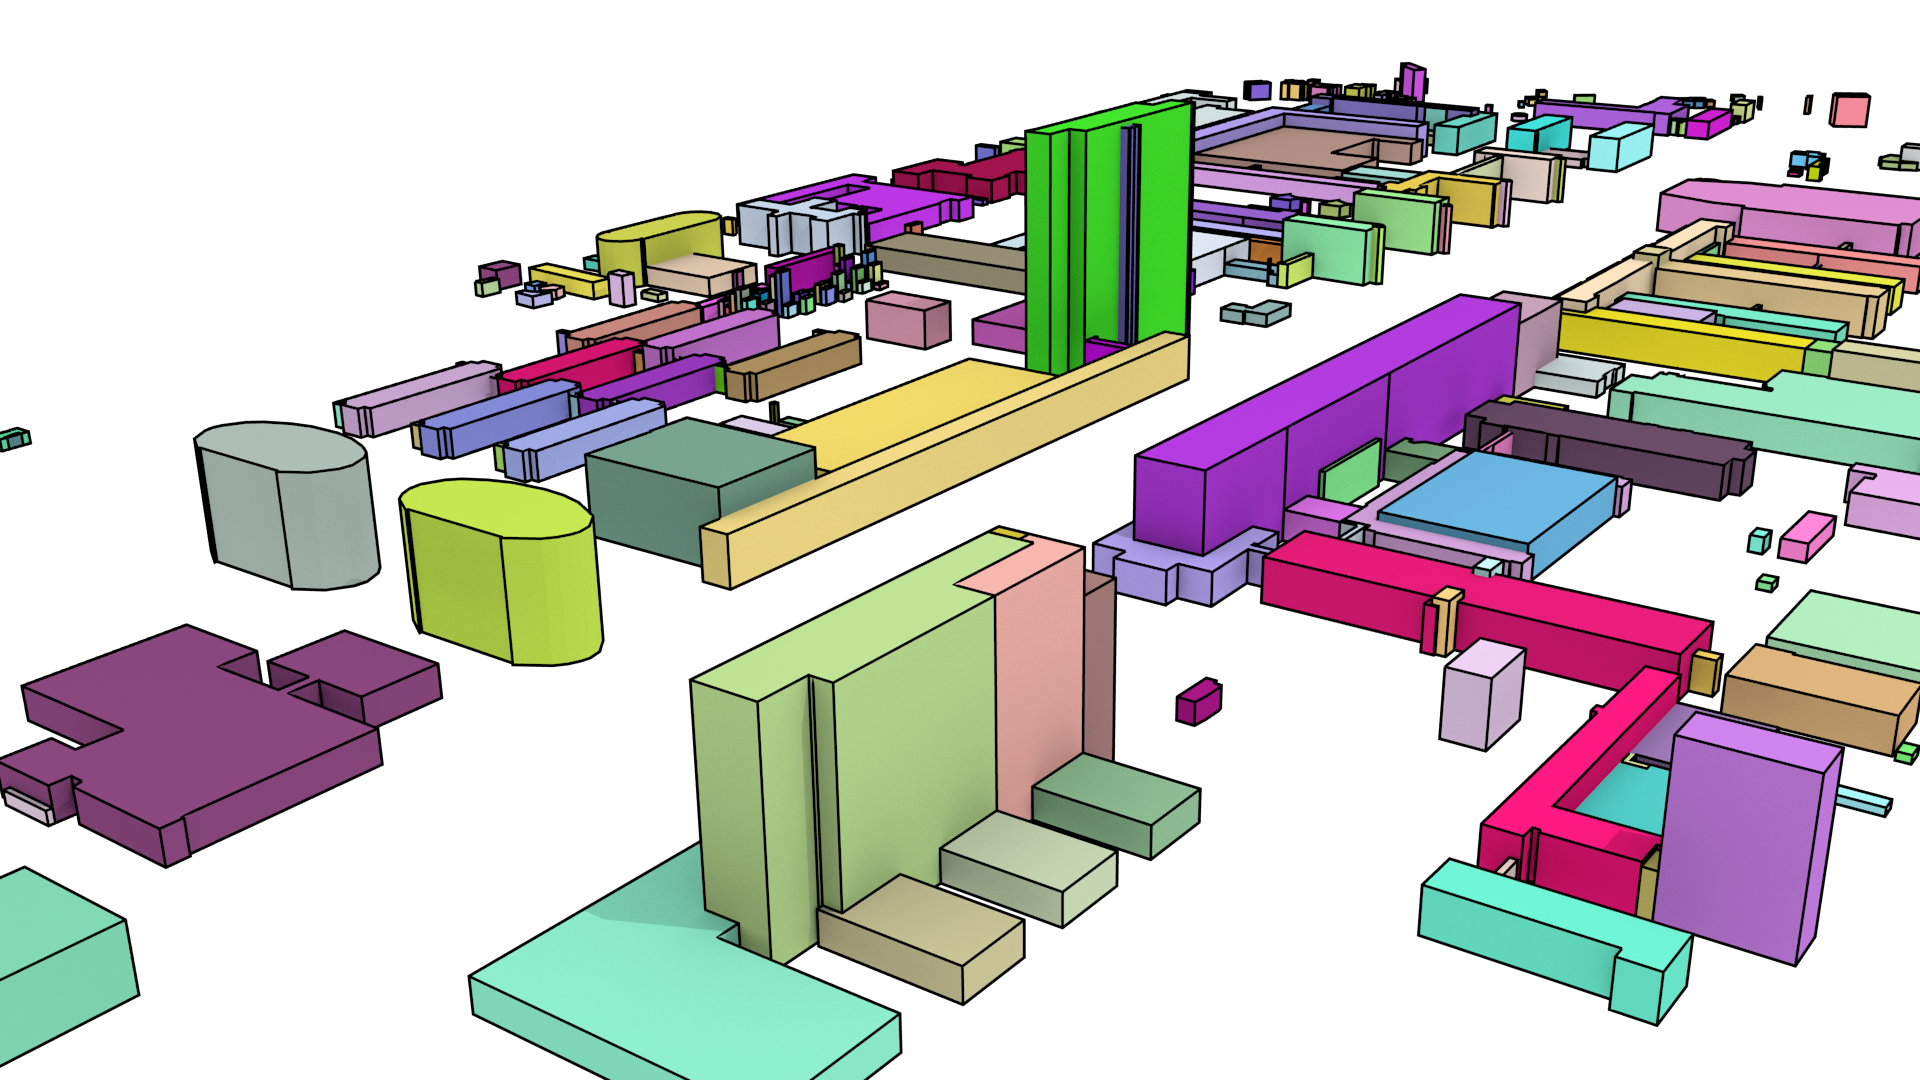
\includegraphics[width=\linewidth]{figs/cellscampus}
\caption[The TU Delft campus as a 3D cell complex]{The buildings in the TU Delft campus are represented as a 3D cell complex. All the 2-cells of a 3-cell are shown in the same colour, the 1-cells are shown as black lines.}
\label{fig:cellscampus}
\end{figure*}

A $j$-dimensional face ($j$-face) of an $i$-cell is a $j$-cell, $j \leq i$, that lies on the boundary of the $i$-cell.
A facet of an $i$-cell is an $(n-1)$-face of the cell.
As in a simplicial complex, two $i$-cells are said to be adjacent if they have a common facet, and an $i$-cell and a $j$-cell, $i \neq j$, are said to be incident if either is a face of the other.
In the context of an $i$-dimensional cell complex, a face refers to each of the $i$-cells in the complex, such as the polygons in a polygonal mesh.

More formally, a cell complex can be defined inductively as in \citet{Hatcher02}.
An $n$-dimensional cell complex is built by starting from a set of isolated vertices, and $\forall 0 < i \leq n$ an $i$-cell is built by attaching itself to the $(i-1)$-faces (facets) on its boundary, these facets having been previously added to the complex.
That is, an edge is built by linking the vertices on its boundary, a surface by linking the edges on its boundary, a volume by linking the surfaces on its boundary, and so on.
Like in a simplicial complex, a facet of a $n$-cell in an $n$-dimensional cell complex lies between it and an adjacent $n$-cell, unless it is on the boundary of the complex.

Apart from the concepts of adjacency, incidence and other relationships between between individual simplices and cells in a complex, it is also possible to define relations and transformations between entire simplicial/cell complexes.
The \emph{Poincar\'e duality} theorem \citep{Poincare93}\footnote{It was only formulated as an observation without proof in \citet{Poincare93}. \citet{Poincare95} describes it in more detail but contains a flawed proof.
Valid proofs would have to wait until \citet{Poincare99,Poincare00}.} states that for every $n$-dimensional simplicial/cell complex, there exists a \emph{dual simplicial/cell complex} of the same dimension, where for every dimension $i$, the $i$-simplices/cells in the original complex are mapped one-to-one to $(n-i)$-simplices/cells in the dual complex.
The \emph{duality transformation} is an operation that creates the dual of a simplicial/cell complex.
This can be seen as a generalisation of the concept of a dual graph in 2D, where a graph $G$ has a dual $G^\ast$, such that vertices in $G$ correspond to faces in $G^\ast$, edges in $G$ correspond to edges in $G^\ast$ and faces in $G$ correspond to vertices in $G^\ast$.

For example, considering the Platonic solids in \reffig{fig:ps}, the tetrahedron is self-dual (\ie\ it is dual to itself), the octahedron is dual to the cube (and vice versa), and the dodecahedron is dual to the icosahedron (and vice versa).
\begin{figure}[tbp]
\centering
\subfloat[]{
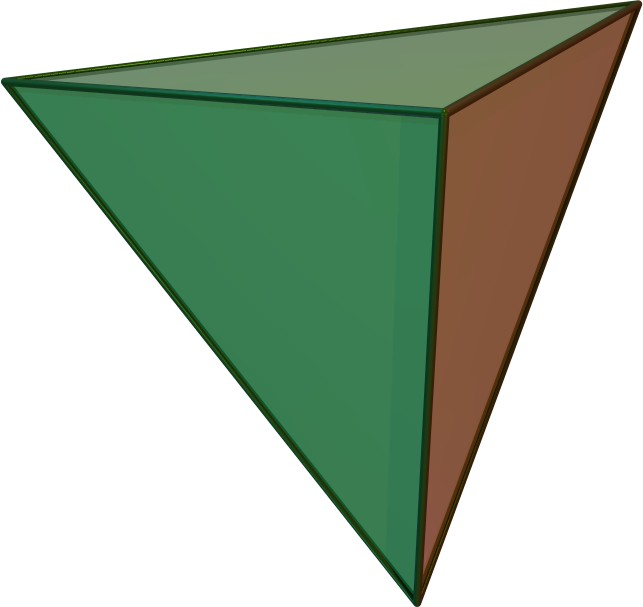
\includegraphics[width=0.15\textwidth]{figs/ps_tetrahedron}
\label{subfig:ps-tetrahedron}}
\quad
\subfloat[]{
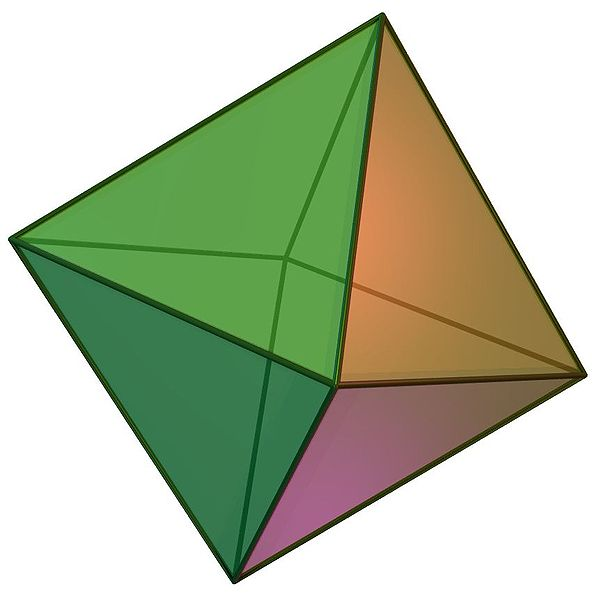
\includegraphics[width=0.15\textwidth]{figs/ps_octahedron}
\label{subfig:ps-octahedron}}
\quad
\subfloat[]{
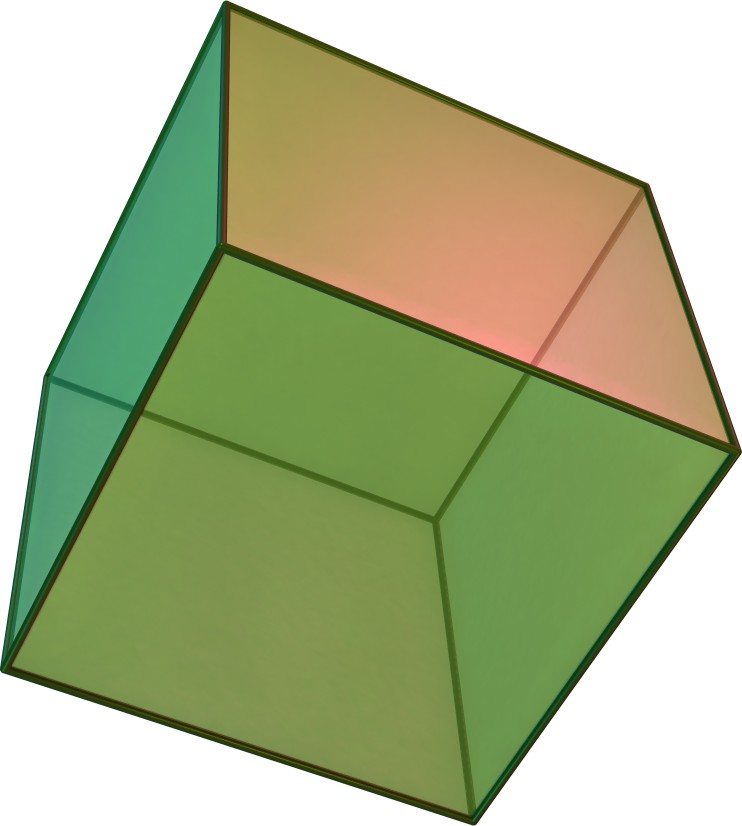
\includegraphics[width=0.15\textwidth]{figs/ps_hexahedron}
\label{subfig:ps-hexahedron}}
\quad
\subfloat[]{
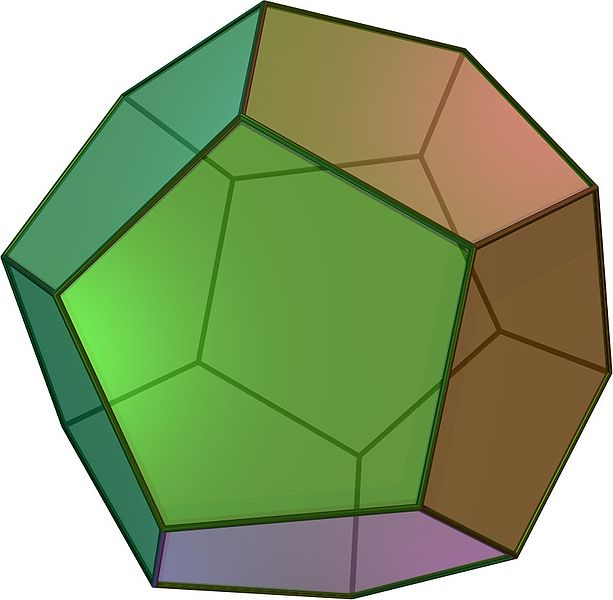
\includegraphics[width=0.15\textwidth]{figs/ps_dodecahedron}
\label{subfig:ps-dodecahedron}}
\quad
\subfloat[]{
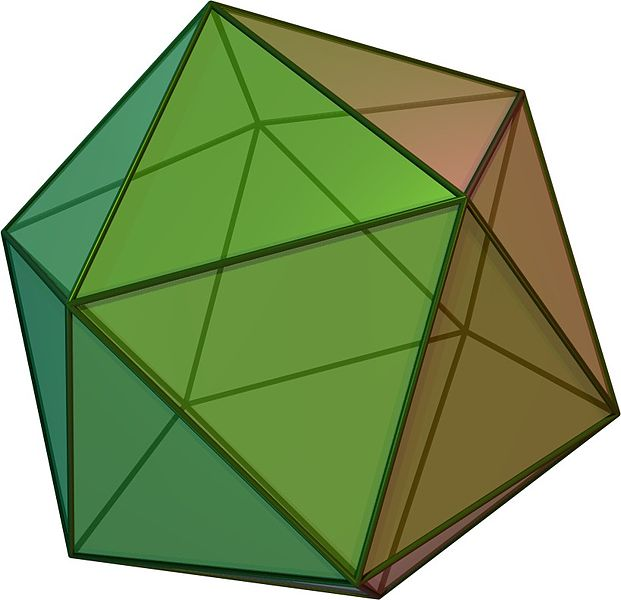
\includegraphics[width=0.15\textwidth]{figs/ps_icosahedron}
\label{subfig:ps-icosahedron}}
\caption[The Platonic solids]{The Platonic solids are the five regular polyhedra that have regular polygonal faces: (a) tetrahedron, (b) octahedron, (c) cube or hexahedron, (d) dodecahedron, and (e) icosahedron. From Wikimedia Commons.}
\label{fig:ps}
\end{figure}
This transformation can be seen by creating a new vertex at the centre point of the face of the Platonic solid, connecting these vertices when their dual faces are adjacent.
The original vertices become faces whose number of vertices is equal to the number of originally incident faces.

% !TEX root = thesis.tex

\chapter{Modelling of 2D/3D space, time, scale and attributes}
\label{ch:modelling-background}

This chapter describes how space is usually modelled in 2D/3D GIS and related disciplines, as well as the non-spatial characteristics that are typically used together with it, such as time and scale.
% With a view to higher dimensions
\refse{se:spatial-modelling} explains what spatial modelling is and the abstraction process through which it is accomplished, discussing the main approaches that can be followed at three levels in this abstraction process, which take the form of data models, data structures and dual combinatorial/embedding structures.
\refse{se:modelling-space} describes how 2D and 3D space is currently modelled in a range of representative concrete cases, from the very minimal representations used in exchange file formats, in which simple structures and low storage requirements are preferred, up to those used internally in CAD-like software, in which the complex operations that are required entail the explicit storage of precise topological relationships.

Afterwards, this chapter contains sections on how specific non-spatial characteristics---that nevertheless have a strong link to space---are modelled: time in \refse{se:modelling-time}, and geographic scale or the level of detail of a model in \refse{se:modelling-scale}.
Finally, \refse{se:modelling-conclusions} concludes the chapter by pointing out some of the shortcomings of the aforementioned approaches to model 2D/3D space, time, scale and attributes.
As will be seen in \refch{ch:nd-modelling}, many of these shortcomings can be resolved by using a higher-dimensional modelling approach.

\section{Spatial data models and data structures}
\label{se:spatial-modelling}

Spatial modelling aims at the creation of digital representations of real-world objects.
However, real-world objects are complex and vaguely defined, while computers can only operate on their heavily abstracted and precisely defined digital counterparts.
The spatial modelling process therefore uses a series of progressive abstractions, which start by interpreting reality as a set of high-level concrete entities that still resemble real-world objects and processes, and ultimately aims at creating abstract low-level representations that are close to a computer implementation, possibly using intermediate levels in the process.

This implies the existence of different levels of abstraction, and at each of these levels different approaches can be followed.
While not all of these approaches are compatible with each other, the feasible combinations nevertheless result in a very large number of different computer representations.

As \refse{ss:taxonomies} explains, there are many classification schemes that attempt to group these approaches in a meaningful way according to various criteria, finding similarities and identifying schemes used by more than one representation.
However, there is no agreement on the optimum number of levels of abstraction to be used, at which level some of these representational choices fit, nor a comprehensive clear-cut classification of them with no overlapping methods.
In fact, as many of these choices only partially solve the difficulties of representing a digital object, a single computer system generally must resort to multiple methods.
For instance, implicit (high-level) models are often used as a way to provide easy user interaction in software.
However, these generally have to be `evaluated' into another, more explicit (low-level) model in order for them to be visualised \citep{Mantyla88} or to perform the type of computations expected in GIS, such as many spatial analysis and geometric operations.

Nevertheless, recognising this layered approach as the basis of the spatial modelling process, this section introduces the process by describing the main approaches that can be followed at three different levels: high-level \emph{data models} using different paradigms to structure and discretise space in \refse{ss:data-models}, how \emph{data structures} implement these data models to model 2D/3D space in a form that is easy to implement in a computer in \refse{ss:data-structures}, and how \emph{combinatorial and embedding structures} respectively model the topological and geometric information of some of these data structures in \refse{ss:combinatorial-embedding}.

\subsection{Classifications of spatial models}
\label{ss:taxonomies}

Considering that there is an incredible variety of methods that are used to create digital models of the world, but many of these share important parts of their respective approaches, there are various classifications that attempt to group them in a meaningful way.

Some of these are primarily based on human cognition of space.
\citet{Couclelis92} distinguishes views based on empty space populated by discrete \emph{objects} from those based on continuous space-filling \emph{fields}, and \citet{Goodchild92} links objects and fields to specific computer models that are suitable for them.
\citet{Freundschuh97} makes distinctions based on the \emph{scale} of such models compared to how people experience space, separating models of objects that are intuitively manipulatable by humans from those that are not.

Others are based on suitability for a particular application or use case.
For example, \citet{Afyouni11} does so for indoor navigation, \citet{Gold05} for multidimensional GIS, \citet{Dominguez11} for building interiors and \citet{Pelekis04} for spatio-temporal models.

However, for the purposes of this thesis, it is more interesting to consider the classifications that reflect a different discretisation of space or mathematical basis, as these will produce significantly different computer representations.

Regarding general classifications in the GIS domain, researchers and practitioners alike generally agree on the existence of two high-level \emph{data models}---formalised structures describing the world as abstract primitives---, which are the \emph{vector} and \emph{raster} models. 
These are subdivided into a variety of low-level \emph{data structures}, particular implementations of these data models, of which there are many \citep{vanKreveld97a}.
This classification is not ideal as GIS data structures are usually specified in an ad hoc manner, sometimes accompanied with added indexing structures that do not neatly fit into the vector or raster approach (\eg\ R-trees \citep{Guttman84} and $k$-d trees \citep{Bentley75}).

Apart from data models and data structures, some authors consider additional levels.
\citet{Frank92} considers \emph{spatial concepts} as well, the human notions used to understand space.
\citet{Peuquet84} considers \emph{reality} itself as a topmost level, including all aspects that may or may not be perceived by individuals, and a lowermost level with the \emph{file structure}, describing how the information is actually represented in hardware.

In the domain of geometric modelling and computer graphics, the schemes used are more varied, and thus the classifications used differ significantly.
For 3D objects, there is usually a high-level classification with several \emph{solid representation schemes} \citep{Requicha80,Hoffmann92,Foley95}, general paradigms to model the world using a different approach to discretise and decompose objects.
As these normally do not reach the level where it is possible to unambiguously devise a single computer implementation, these are more akin to the data models used in GIS.\@
\citet{Mantyla88} follows a similar classification, but groups these schemes into three paradigms: \emph{decomposition models}, \emph{constructive models} and \emph{boundary models}, while recognising the existence of hybrid approaches combining multiple paradigms.

While some of these schemes use 3D primitives stored as simple parametric structures, many of them rely on the specification of 2D primitives using a separate mechanism, which can also be used directly for the description of 2D objects.
These are usually described at a low level, generally consisting of 2D cell or simplicial complexes respectively in the form of \emph{polygon} or \emph{triangle meshes}, which use one of a few \emph{data structures} \citep{Joy03,Alumbaugh05,Blandford05,deFloriani05}.

Some authors follow a more pragmatic approach, directly classifying data structures based on the class of objects that they are capable of representing.
\citet{Comic12} does so for cell complexes, \citet{deFloriani05} for simplicial complexes, \citet{Lienhardt91} for spaces in different dimensions, \citet{deFloriani05a} for models supporting multiple levels of detail, \citet{Lienhardt09} for models for simplicial, simploidal\footnote{Cartesian products of simplices} and cell structures.

Finally, at the lowest level, some authors distinguish between a \emph{topological} or \emph{combinatorial model} \citep{Lienhardt91}, which describes the connectivity between a set of predefined elements, and a \emph{geometric} or \emph{embedding model}, which specifies the exact shape and position of individual elements \citep{Mantyla88}.

\subsection{Data models or representation schemes}
\label{ss:data-models}

Data models are considered as different representation schemes operating at a high-level, differing mostly in their overall approach to decompose and discretise space into a set of elements with certain characteristics.
Just as the concepts of geometry and topology seen in \refch{ch:modelling-mathematics}, these models are essentially \emph{dimension-independent}---even if in practice they are generally implemented as dimension-specific data structures.

As argued by \citet{McKenzie01}, the ideal data model to be used depends on the application.
An ideal data model is expected to be both simple and powerful, but unfortunately these properties tend to conflict.
Powerful structures are built upon small and simple primitives of a fixed form with a fixed (or at least bounded) number of links to other related primitives, such as boxes or simplices, enabling them to have a simple but powerful algebra to manipulate them and to navigate between their primitives efficiently, \eg\ the quad-edge in 2D \citep{Guibas85} or the facet-edge in 3D \citep{Dobkin87}.
However, partitioning complex objects into these simple primitives can be difficult and result in a large number of primitives, requiring significant preprocessing, making them space-intensive and limiting the types of objects that might be stored.
In this sense, different data models make different choices and necessarily involve a trade-off.

The main data models are briefly described in the following sections, roughly in order of increasing explicitness.
A short statement on how well they extend to higher dimensions is included in each section.
The most promising of these models are further analysed in a higher-dimensional context in \refse{se:data-structures}.

\subsubsection{Primitive instancing}

In \emph{primitive instancing}, the system defines a library of primitives suitable for a particular application.
Each of the primitives in the library represents a template for an object that can be parametrised in terms of high-level parameters, such as the number of teeth and the size of a gear or the diameter and thickness of a pipe \citep{Foley95}.
In 3D city modelling, a common application involves the modelling of roofs using a library of basic roof shapes (\eg\ flat, hipped and gabled) \citep{Kada07}.

The fact that only a few parameters need to be defined makes it easy to create objects, that is, as long as the desired object resembles one of the templates in the library.
Moreover, given these parameters and a primitive's position and orientation, a program can create the geometry of an object that matches those parameters as output using a more explicit representation.
Such an object can then be used either directly or as a base for further operations.

Usually, the primitives used in primitive instancing are 3D volumetric objects, but they can actually be objects of any dimension.
However, this approach is not practical for higher-dimensional models of geographic information as the objects modelled do not conform to a set of easily parametrisable primitives.

\subsubsection{Sweep representations}

Many objects can be modelled as the space occupied by another object while it is being translated and rotated along a path.
Usually a 2D cross-section is used for this purpose, which is either translated or rotated, generating a volume in 3D space.
Generalisations where the cross-section is deformed as well are sometimes considered \citep{Blackmore94}.
When the path is linear and the cross-section is not rotated, it is called a \emph{translational sweep}, or an \emph{extrusion} as it resembles a physical extrusion process as used in manufacturing.
When the cross-section does not move and it is merely rotated, it is called a \emph{rotational sweep} or a \emph{solid of revolution}.
Among other applications, this representation is particularly convenient for applications that require volume computations as it matches well with calculus techniques to compute integrals, which can be easily solved numerically in a computer \citep{Lee82}.

Since the description of a 2D cross-section is easier than that of a full 3D volume, this significantly eases the process of modelling certain types of objects \citep{Weld90}.
In a higher-dimensional context, this property is later used to generate $n$-dimensional extruded models in \refch{ch:extrusion}.
Generating more general higher-dimensional sweeps and revolutions is also possible using similar methods.

\subsubsection{Constructive solid geometry}

\emph{Constructive solid geometry} (CSG) \citep[\S{}12.3]{Requicha77} represents objects as a tree of regularised Boolean set operations on a set of simple parametrisable primitives.
In most instances, these are volumetric primitives such as balls, cylinders, parallelepipeds, cones and tori.
\reffig{fig:csg} shows an example of such an object.
\marginpar{
\captionsetup{type=figure}
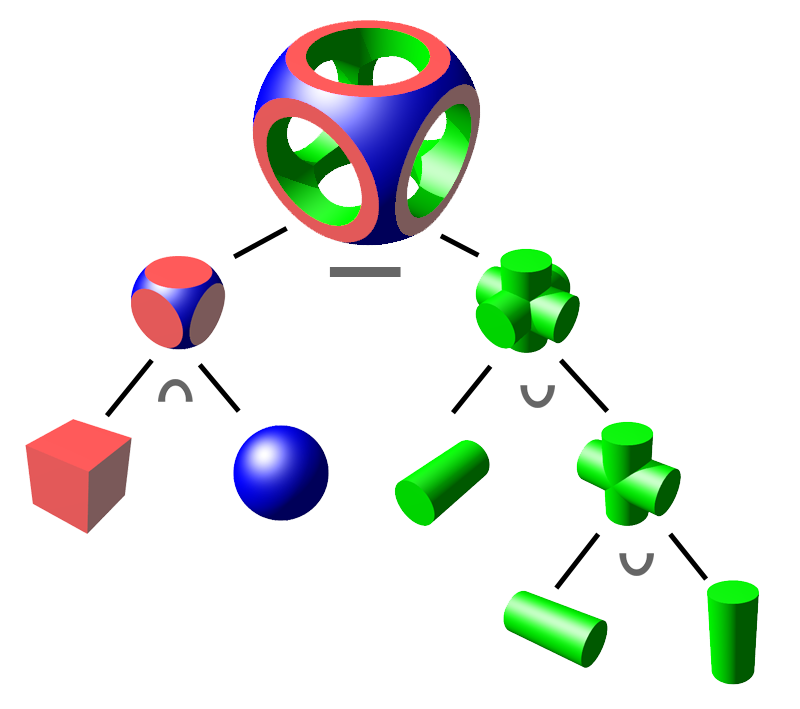
\includegraphics[width=\marginparwidth]{figs/csg}
\caption[An object represented as a tree of Boolean set operations]{An object represented as a tree of Boolean set operations on a sphere, a cube and three cylinders. From Wikimedia Commons.}
\label{fig:csg}
}
CSG is particularly useful since it allows many operations to be distributed among the primitives in a tree.

The regularisation step ensures that the resulting objects of any Boolean set operation are both volumetric and water-tight \citep{Requicha78}, making many computations easy and robust.
It also makes it relatively easy to transform a CSG tree to a more explicit representation.
CSG is therefore used in most CAD software and in many game engines.

While CSG extends naturally to higher dimensions, evaluating general CSG trees into more explicit representations is non-trivial in dimensions higher than three.
A possible approach to do so would involve higher-dimensional Nef polyhedra, which are described below.

\subsubsection{Boolean set operations on half-spaces}

There are various representations that store objects using an expression made of Boolean set operations on a set of (open or closed) half-spaces.
Any convex object of any dimension can be represented as the intersection of a finite set of half-spaces, a common problem in both linear programming and computational geometry \citep{Shamos76,Preparata79}.
As \reffig{fig:halfspace} shows, if a polyhedron is first decomposed into convex parts \citep{Chazelle79,Bajaj90}, it is then possible to represent an object as a union of these convex parts, which are then represented as intersections of half-spaces.
\begin{figure}[b]
\centering
\subfloat[]{
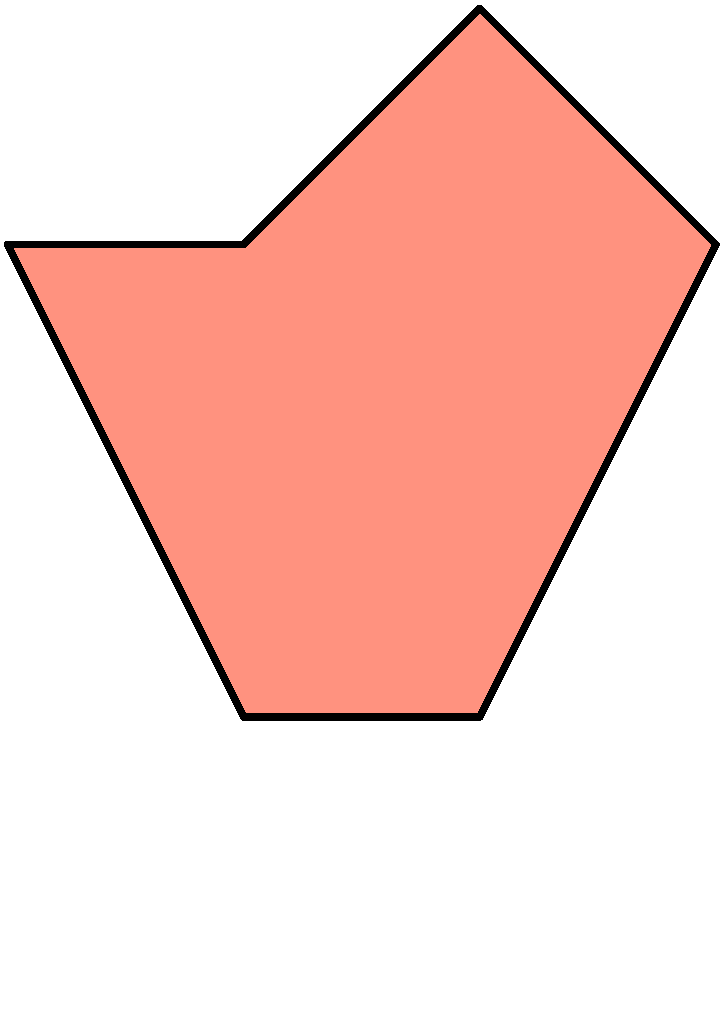
\includegraphics[scale=0.16]{figs/halfspace}
\label{subfig:halfspace}}
\subfloat[]{
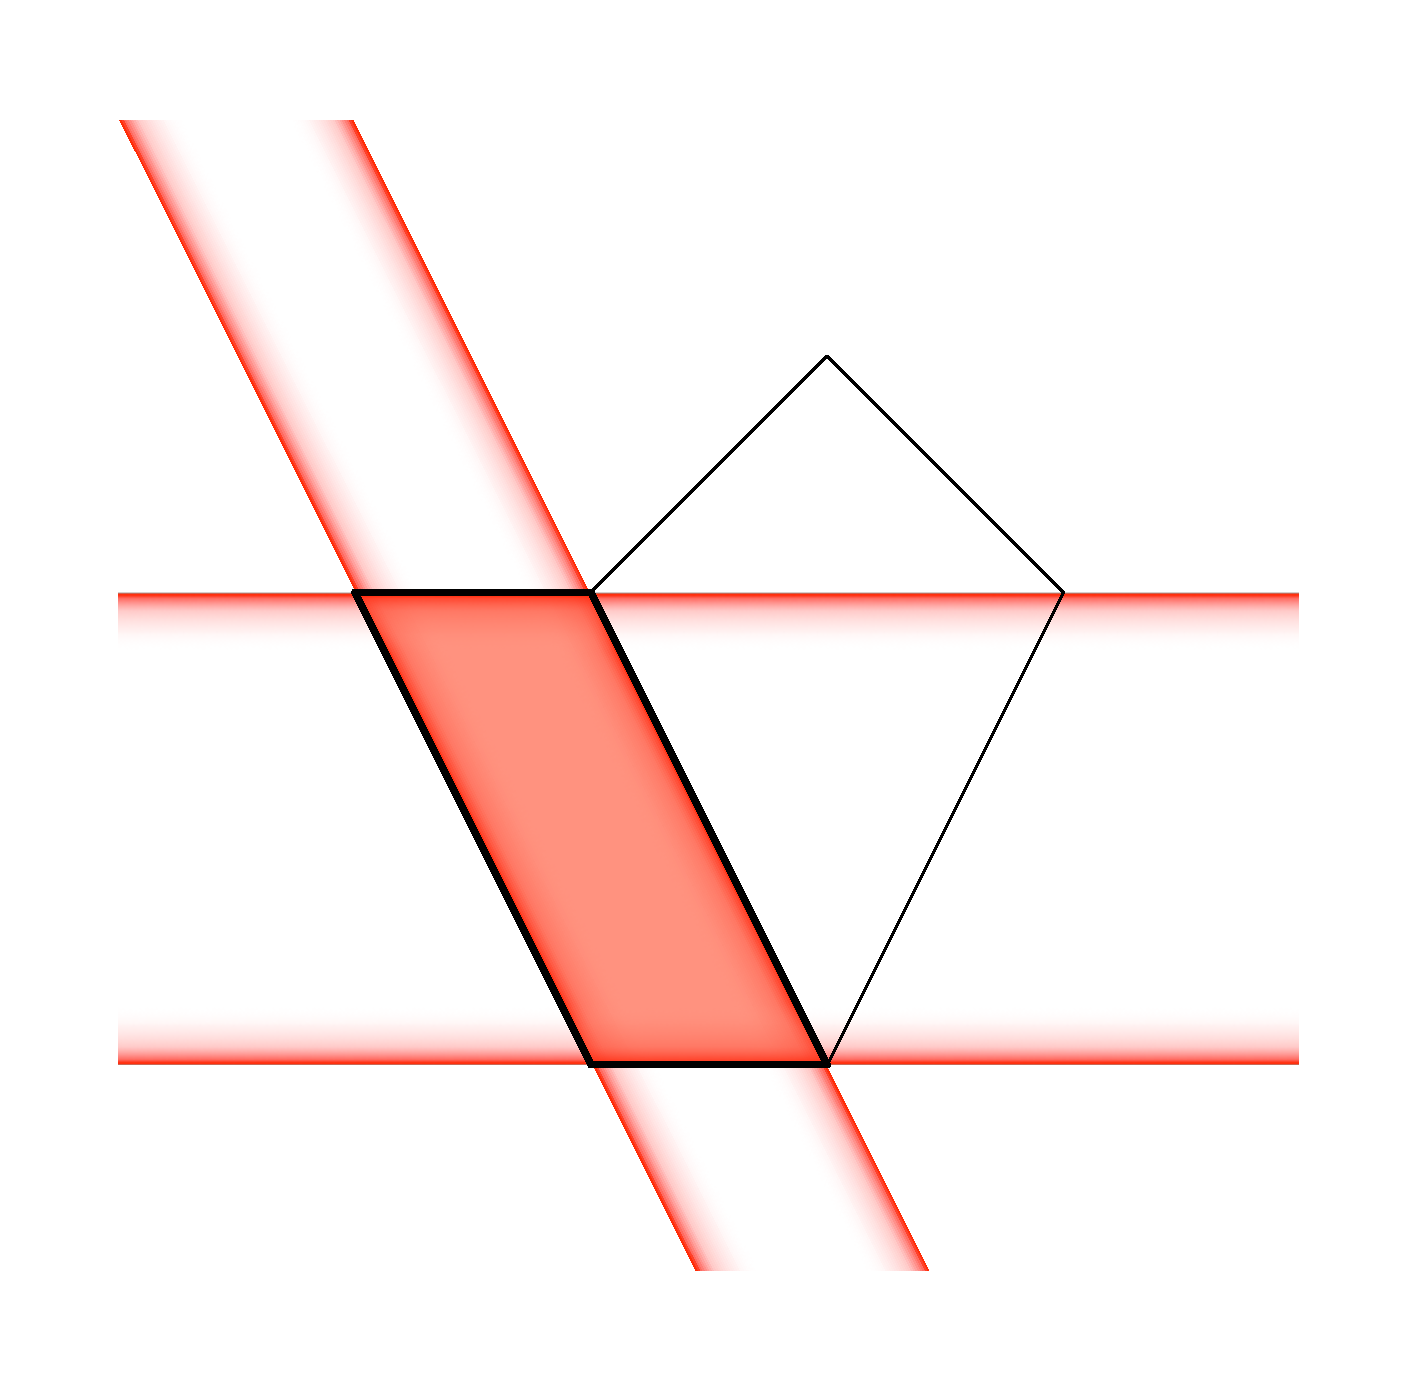
\includegraphics[scale=0.16]{figs/halfspace-1}
\label{subfig:halfspace-intersection}}
\subfloat[]{
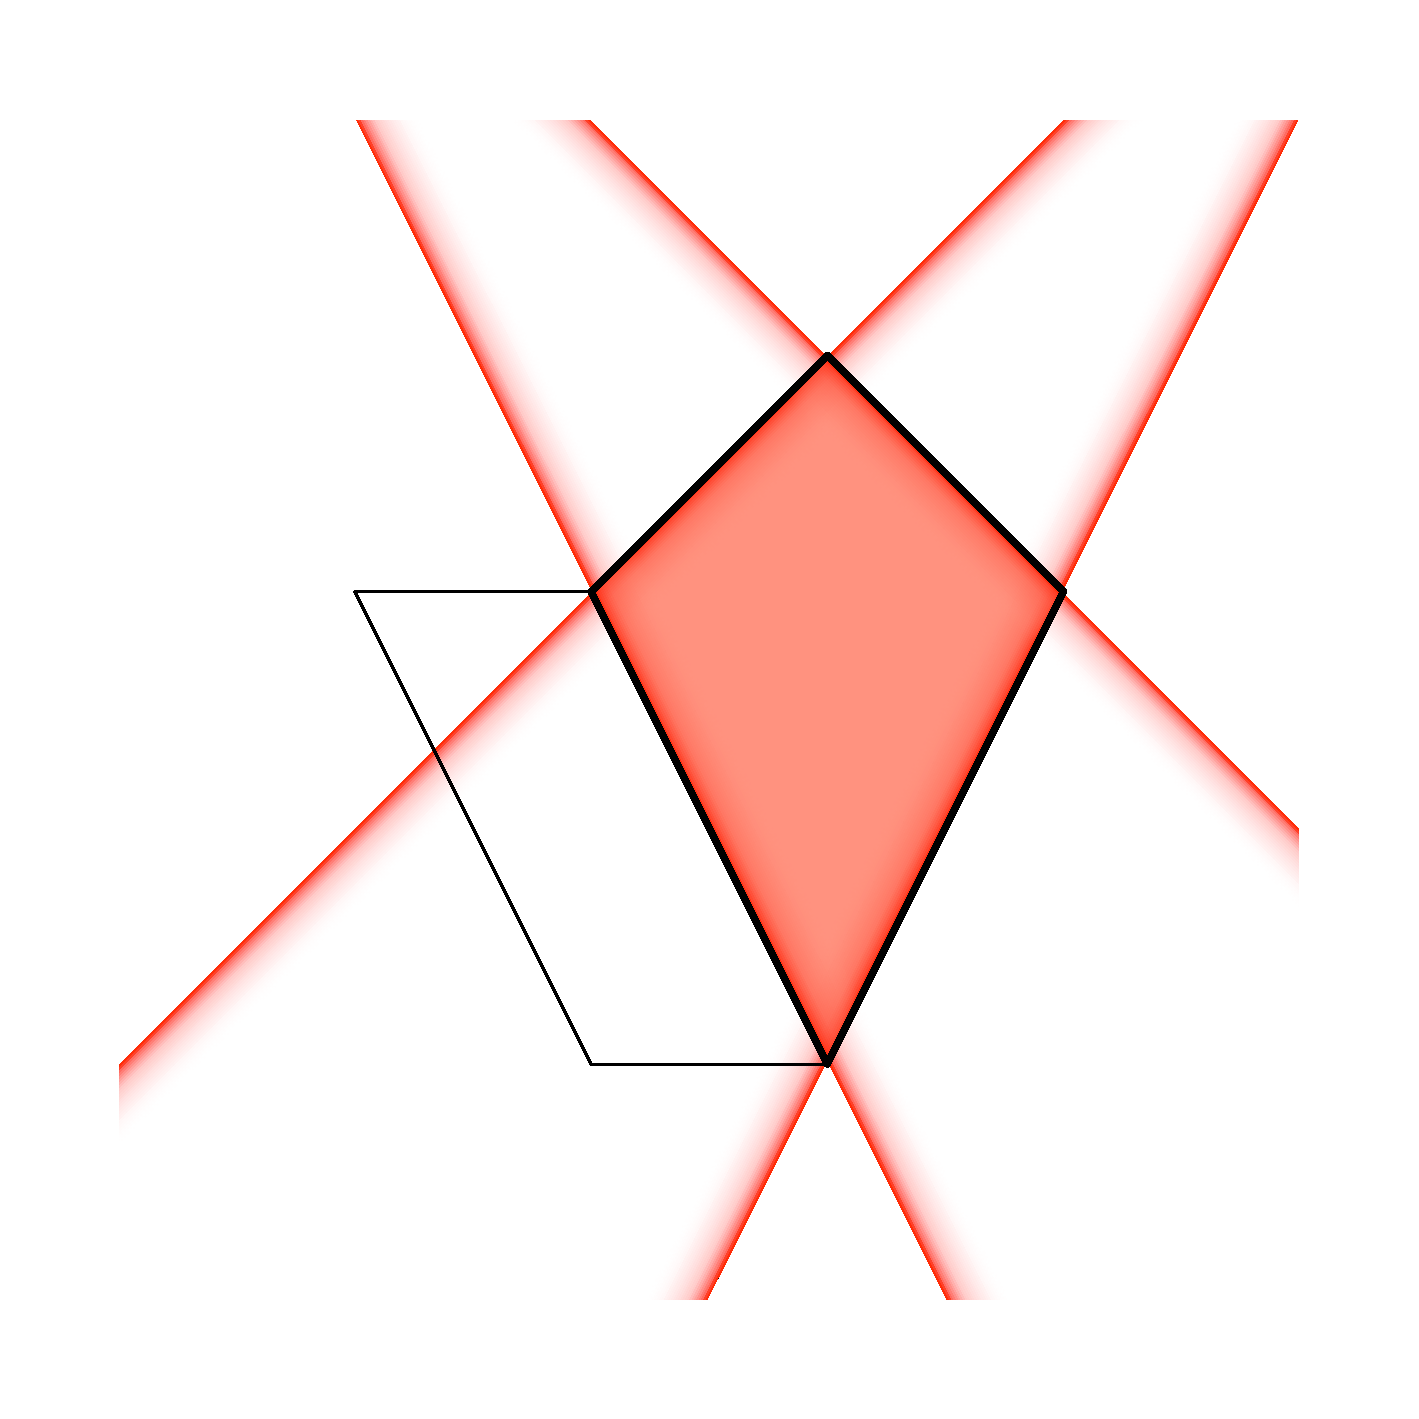
\includegraphics[scale=0.16]{figs/halfspace-2}
\label{subfig:halfspace-union}}
\caption[A polygon represented as the union of two convex polygons]{(a) A polygon can be represented as the union of its decomposition into the convex polygons (b) and (c). Each of these can then be represented as the intersection of four half-planes.}
\label{fig:halfspace}
\end{figure}

Each of these half-spaces can then be stored easily, \eg\ as a tuple containing the coefficients of a hyperplane\footnote{\ie\ a line in 2D and a plane in 3D.} equation plus an up/down direction \citep{Naylor90,Thompson07}.
The half-spaces for an object can be stored either all together or separate per convex part.
Together, for instance, as a collection of plane equations that represent all the faces of all the convex parts, and each convex part is represented as a set of tuples of Boolean values, where each value states whether the part is on the up or down side of a specific plane \citep{Tammik07}.

\subsubsection{Nef polyhedra}

Nef polyhedra \citep{Nef78,Bieri88} follow a similar approach to half-space models, but extend it with the concept of a local $n$-dimensional pyramid\footnote{This is equivalent to a triangle in 2D and a polyhedral pyramid in 3D.}, which stores the neighbourhood information around every vertex.
As \reffig{fig:nef} shows, the local pyramid of a vertex thus contains the symbolic intersection of an infinitesimally small sphere (in 3D) or circle (in 2D) with the volumes, faces and edges incident to this vertex.
\marginpar{
\captionsetup{type=figure}
\centering
\subfloat[]{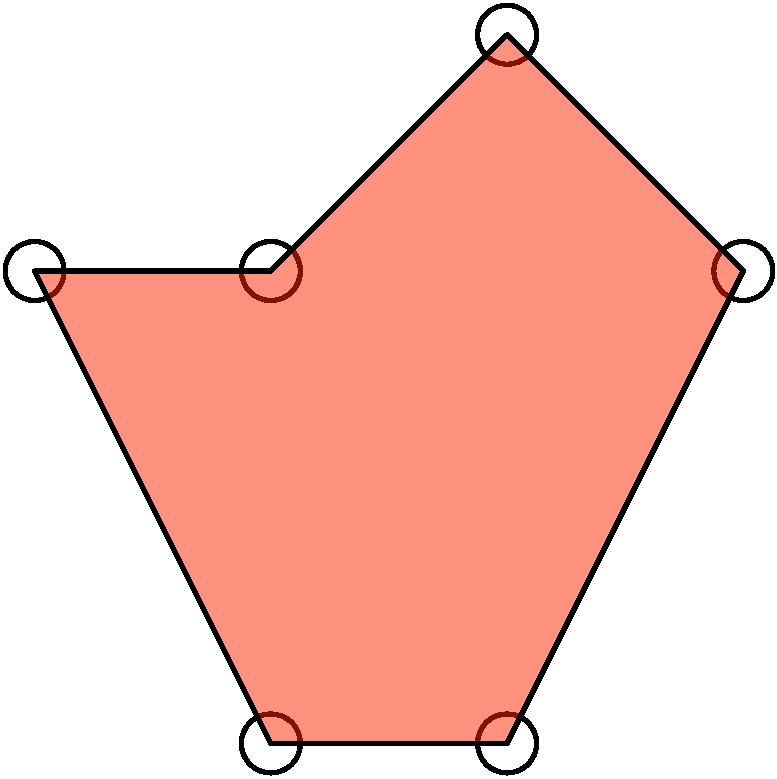
\includegraphics[width=\marginparwidth]{figs/nef-1}} \\
\subfloat[]{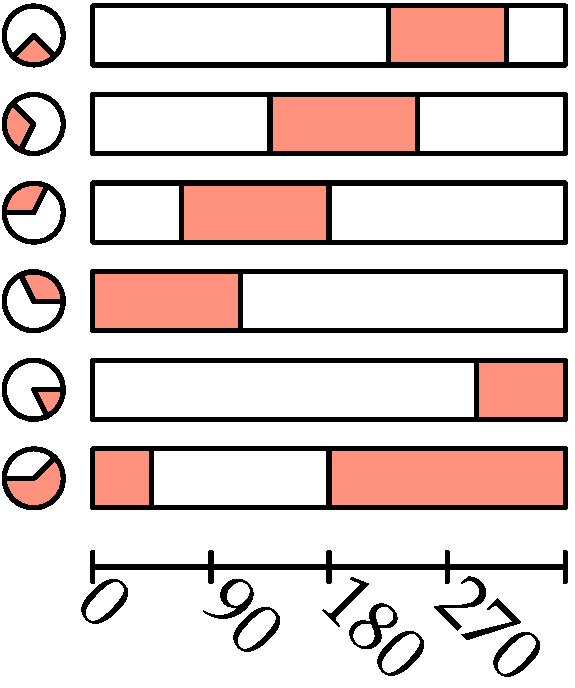
\includegraphics[width=0.7\marginparwidth]{figs/nef-2}}
\caption[A Nef polygon represented by a set of local pyramids]{(a) A Nef polygon is represented by (b) a set of local pyramids (circles). At every local pyramid, the polygon (grey) becomes an angular interval. Incident edges become points at the endpoints of these intervals.}
\label{fig:nef}
}
An incident volume thus becomes a face, an incident face becomes an edge, and an incident edge becomes a vertex on the surface of the local pyramid sphere/circle, essentially lowering the dimension of every object by one.
An 2D/3D object can be represented as a set of local pyramids, which can individually be stored using simpler 1D/2D data structures.

Nef polyhedra have two properties that make them very interesting representations for higher-dimensional models of geographic information: (i) the possibility to reduce the dimensionality of a representation by one, which can be applied recursively in order to model objects of any dimension, and (ii) the possibility to perform operations on the local pyramid level.
The former is discussed in more detail in \refse{ss:implicit-models} and the latter in \refse{ss:operations-nef}.

\subsubsection{Function representation}

Function representation, commonly abbreviated as F-rep, involves representing objects as point sets using an arbitrary continuous function \citep{Pasko95}, which is represented as an algebraic expression.
When a given function $f(x_0, x_1, \ldots, x_n)$ is evaluated at a point with coordinates $(x_0, x_1, \ldots, x_n)$, it is possible to know if the point lies in the interior, boundary or exterior of an object.
If it is positive the point is in the interior of the object, when it is zero it is on the boundary of the object, known as an isosurface, and when it is negative it is outside the object.

By varying the number of input parameters, which in most cases represent a point along an axis, function representations are applicable to any dimension.
Moreover, unlike a half-space inequality, such functions do not need to be linear.
As with half-space based representations, the spaces described by these functions can be combined using Boolean set operations, which is done on the basis of Rvachev functions (R-functions) \citep{Rvachev63}.
However, evaluating these functions in higher dimensions can be complex, and obtaining a continuous function that adequately models a higher-dimensional object is also non-trivial.

\subsubsection{Exhaustive enumeration}

Starting from the description of a domain that covers the objects that need to be described, a simple deterministic rule is used in order to partition the domain directly into cells, which are of the same dimension as the domain (\ie\ space-filling).
In this manner, the decomposition rule is encoded into the model rather than in the data being represented, and so the cells do not need to store any geometric information of their own.
Normally, the domain has a simple shape (\eg\ a rectangle, hexagon or box) \citep[\S{}6.8]{ISO19123:2007} and the rule partitions it into simple cells of the same size and shape (\eg\ rectangles or boxes themselves), in which case it is called a \emph{monohedral} tessellation \citep{Boots99}.
If the cells are regular polygons or polyhedra, it is known as as \emph{regular} tessellation.

In most cases, squares or rectangles (in 2D) and cubes or parallelepipeds (in 3D) are used for simplicity, respectively resulting in pixel and voxel structures.
When other shapes are used, it is normally desirable to have cells that resemble equally-sized disks or balls as much as possible, something that is related to the sphere packing or kissing number problems in geometry \citep{Conway92}.
\emph{Semi-regular} tessellations, which consist of more than one type of polygon/polyhedron are also possible but are not widely used, even in 2D.
In 2D, the most commonly used other shapes are triangles and hexagons.
In 3D, parallelepipeds or cubes are almost always used, but the face-centred cubic or hexagonal close-packed lattices are possibilities that resemble balls more closely.

These cells are then used to record whether the cell belongs to the interior of the object or not, or in the case of multiple objects, which objects are present inside the cell.
After such a tessellation is defined, a programatic order or path that traverses all cells (\ie\ a space filling curve) is defined \citep{Sagan94}, and the order of the cells along this curve is used to store them by \emph{enumerating} for each cell whether a cell belongs to the interior of an object.

Exhaustive enumeration schemes are straightforward to extend to higher dimensions, as is further discussed in \refse{ss:regular-partitions}, with the caveat that their space complexity can increase exponentially on the dimension.

\subsubsection{Hierarchical subdivisions using trees}

A more general possibility to partition a domain involves using a hierarchical scheme where a space is recursively subdivided according to a particular criterion, resulting in a tree structure where a given node is a partition primitive that divides the space defined by its parent.
Such structures are generally known as space partitioning trees.
In this manner, it is possible to efficiently partition spaces of any dimension, including areas and volumes where the objects' sizes are significantly different.
However, the shape of a cell in the subdivision is only known after traversing a complete branch of the tree from its root to the leaf corresponding to the cell.

In the simplest case, the space can be split evenly into halves along all axes at every partition node, resulting in a \emph{quadtree} in 2D \citep{Finkel74} or an \emph{octree} in 3D \citep{Meagher80}.
Bintrees \citep{Samet85} partition space alternating among dimensions rather than all at once, while $k$-d trees \citep{Bentley75} do so at an arbitrary point rather than at the midpoint of a space.
Many other types of trees however exist.
See \citep{Manolopoulos06}.

As in exhaustive enumeration, this type of representation extends naturally to higher dimensions (\refse{ss:hierarchical-subdivisions}).
The leaves of the tree can be easily used to record whether a cell belongs to the interior of an object or not.

\subsubsection{More general cell decompositions}

Another possibility to represent the geometry of an object involves its decomposition into cells that are more complex than those in the exhaustive enumeration approach, such that they are still of the same dimension as the domain being partitioned but might have different sizes and/or shapes.
Nevertheless, they should still be describable as single computer primitives.
This requires geometric information to be stored within each cell (\eg\ the coordinates of one or more points).

While an arbitrary number of cell decomposition schemes are possible, the most interesting ones in a dimension-independent context are $n$-dimensional constrained triangulations and Voronoi diagrams, as these have a simple dimension-independent formulation.
2D constrained triangulations \citep{Chew89,Shewchuk96} and 3D constrained tetrahedralisations \citep{Si05} are very commonly used in GIS in order to subdivide objects respectively into triangles and tetrahedra, resulting in models that can be represented as simplicial complexes where every simplex can be respectively described by three and four linearly independent points at their vertices.
Another common possibility uses Voronoi subdivision described by a single point per cell \citep{Voronoi08}, something that is particularly suitable to field-like GIS data \citep{Ledoux06}.

More information on how simplicial complexes are stored in 2D and 3D GIS is given in \refse{ss:data-structures}.
\refse{ss:simplicial-complexes} later describes how this extends readily to higher dimensions.

\subsubsection{Incomplete (implicit) models}

Incomplete models attempt to describe a space partition based on implicit rules applied to lower-dimensional primitives only, usually for simplicity purposes.
As such, the actual cells forming the partition are created on the fly.
Under some circumstances, such as when modelling non-manifolds or when the dimension of the primitives is significantly lower than that of the highest-dimensional cells, they cannot be unambiguously described.

The most typical problematic examples are wireframe models in 3D, which represent volumes using only vertices and edges.
While in many cases it is possible to correctly interpret a volume from a wireframe model \citep{Brewer86,Hanrahan82}, as shown in \reffig{fig:wireframe} there are cases wireframe representations are ambiguous.
\begin{figure}[tbp]
\centering
\subfloat[]{
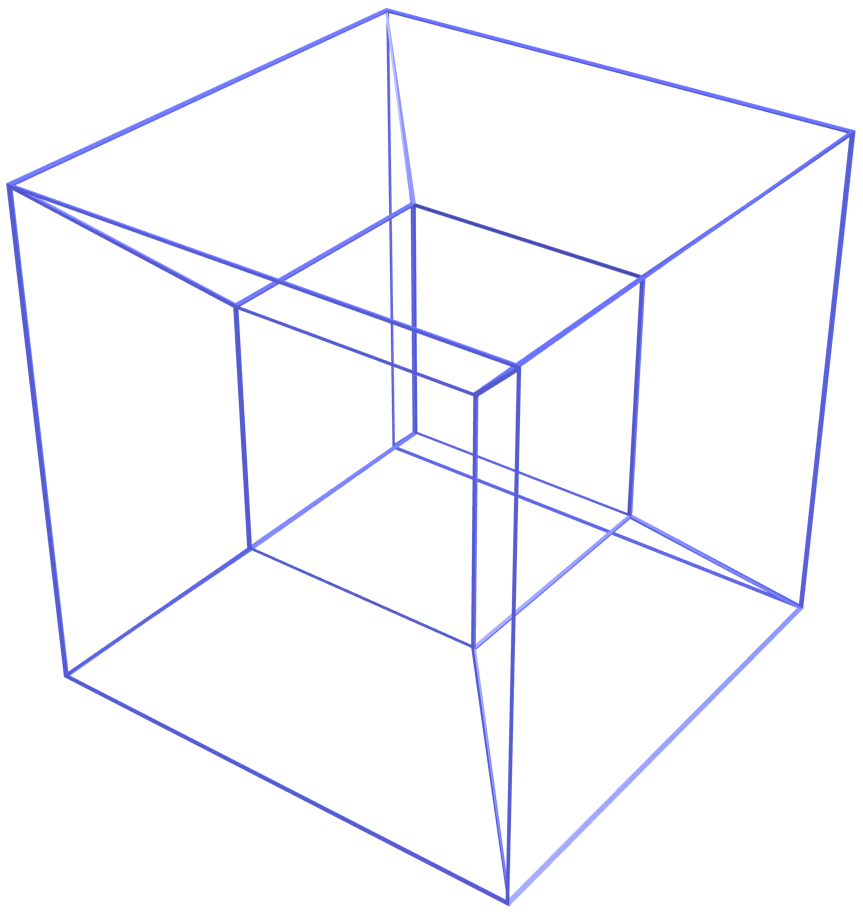
\includegraphics[width=0.35\linewidth]{figs/wireframe}
\label{subfig:wireframe}}
\quad
\subfloat[]{
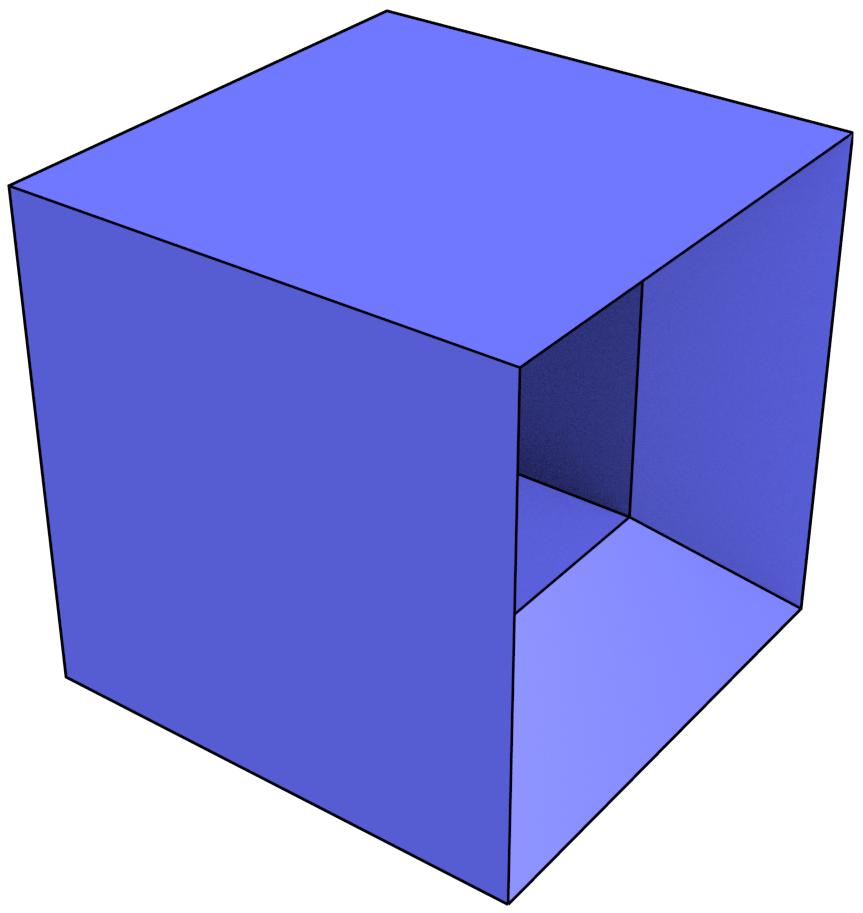
\includegraphics[width=0.35\linewidth]{figs/wireframe-1}
\label{subfig:wireframe-1}}
\\
\subfloat[]{
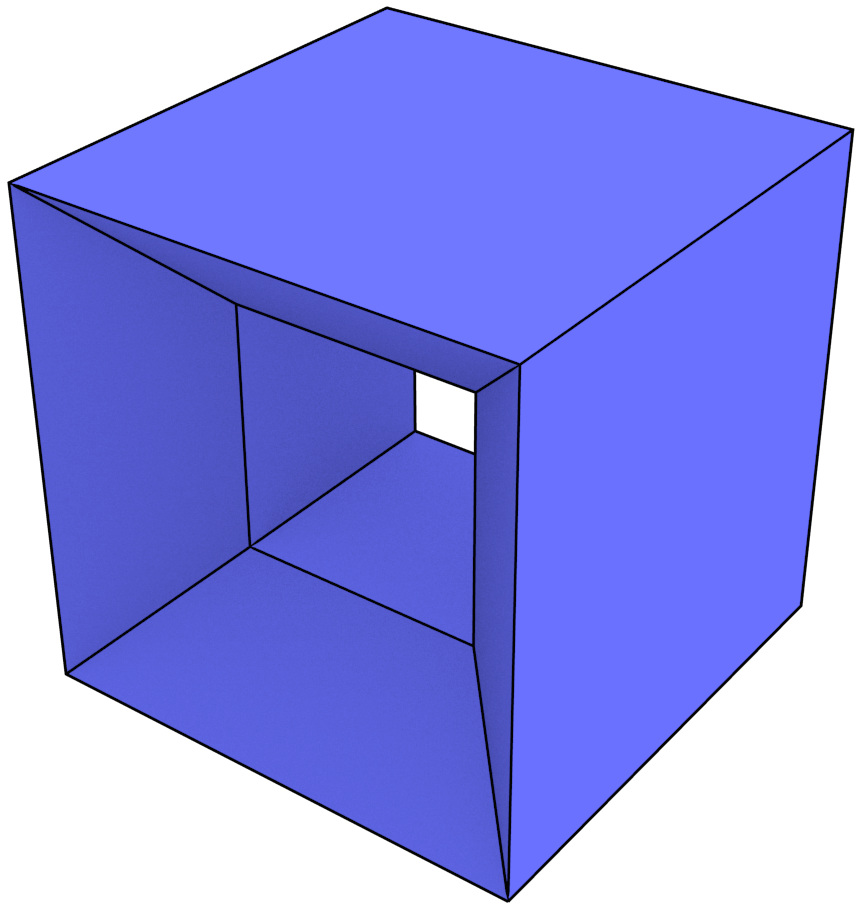
\includegraphics[width=0.35\linewidth]{figs/wireframe-2}
\label{subfig:wireframe-2}}
\quad
\subfloat[]{
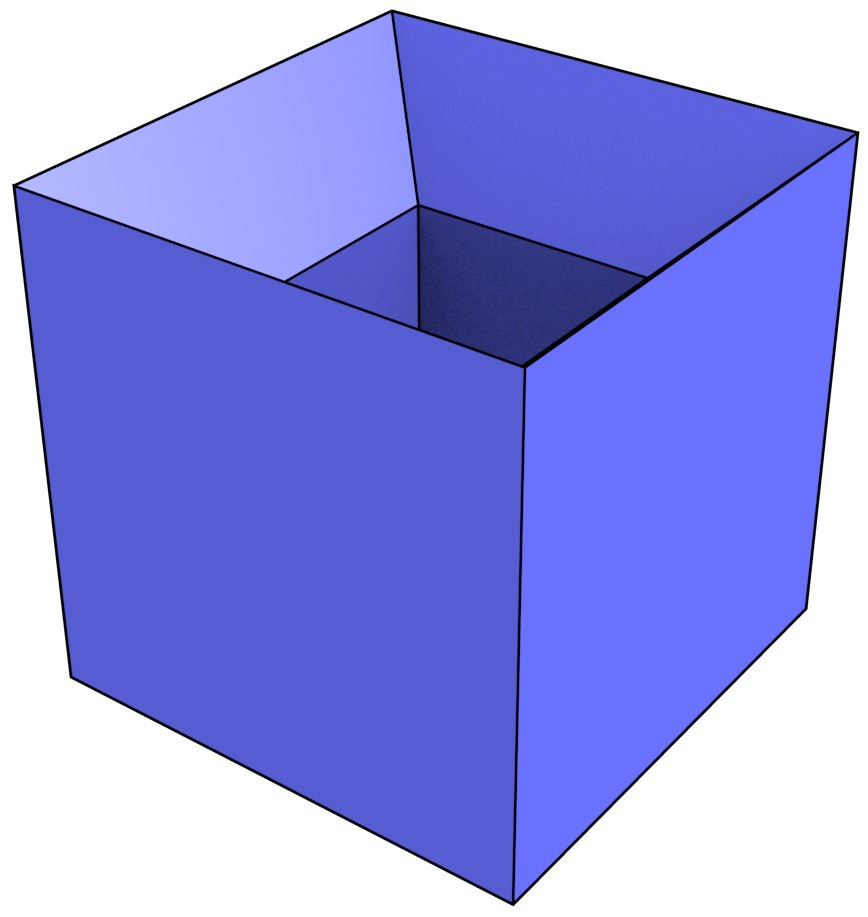
\includegraphics[width=0.35\linewidth]{figs/wireframe-3}
\label{subfig:wireframe-3}}
\caption[A wireframe model can have different interpretations]{(a) A wireframe model that can be interpreted as the three different volumes (b), (c) and (d).}
\label{fig:wireframe}
\end{figure}
They are therefore considered an incomplete representation and are generally not used in current systems.

Despite their drawbacks, incomplete implicit models are however frequently used in 3D GIS and when modelling time, resulting in ill-defined volumes or unclear equivalences of objects across time.
Many of these disadvantages are alluded later on in order to justify using explicit representations in higher dimensions.

\subsubsection{Boundary representation}

Considering the Jordan curve theorem \citep{Jordan87}, which states that a closed curve separates the plane (\ie\ $\mathbb{R}^2$) into two parts: an \emph{interior} shape and an \emph{exterior} shape, it is possible to use this curve in order to \emph{implicitly but unambiguously} represent the interior (or exterior) shape.
This theorem was generalised to higher dimensions as the Jordan-Brouwer theorem by \citet{Lebesgue11,Brouwer11}\footnote{This is somewhat contentious. See \citet[Ch.~5]{van-Dalen13}.}, implying that a volume in $\mathbb{R}^3$ can be represented by the 2D boundary surface that separates its interior from its exterior.
This method, known as \emph{boundary representation}, \emph{B-rep} or \emph{surface modelling}, reduces the complexity of the problem by making it possible to use 2D data models/structures to store 3D objects, which are significantly simpler.
Moreover, by decomposing the 2D surface into simple cells, \eg\ triangles or polygons, it becomes possible to represent the surface using one of the many data structures capable of representing 2D cell complexes, and if these cells support curved domains (\eg\ NURBS), these can be used to represent complex surfaces as well.

While certain problems become more difficult by the use of boundary representation, such as the fact that it is easy to create invalid objects, some others can be performed directly on the 2D cells.
For instance, visibility queries or determining if a point is in the interior of an object can be performed by shooting rays.

As will be discussed in \refse{ss:data-structures} for 2D/3D and \refse{ss:cell-complexes} for $n$D, cell complexes are often represented using boundary representation schemes.
\refse{ss:ordered-topological-models} instead shows how an $n$-dimensional cell complex can be represented using a data structure based on a simplicial complex.
The latter approach arguably combines the benefits of both and used for most of the methods developed in the latter chapters of this thesis.

\subsection{Data structures}
\label{ss:data-structures}

The terms `data model' and `data structure' are often used interchangeably, but within this thesis it is useful to make a distinction between a data model, \ie\ a particular \emph{dimension-independent} discretisation of space into abstract primitives of a certain form, from the data structure(s) used to implement it, \ie\ their representation in a computer-compatible form \citep{Frank92}, which is often \emph{dimension-specific}.
A data model broadly defines the shape of the primitives and relationships that exist between them.
In contrast, a data structure defines a \emph{concrete representation} of these primitives, deciding to \emph{explicitly} store some of these relations and omit others (which can often be computed with an added computational cost).

This distinction is blurred because many data models have very straightforward, natural representations.
Ad hoc data structures used in GIS often define a set of fields that is different per dimension, resulting in awkward definitions at the data model level.
As shown in \refse{se:geometry}, many geometric primitives can be stored on the basis of a set of points or the coefficients of an equation---all of which can be stored as tuples of numbers.
This is also true for the subdivision primitives in cell decomposition schemes and in most cases for the definition of the domain in exhaustive enumeration as well.
Meanwhile, primitive instancing schemes and constructive solid geometry models can be stored as tuples of parameters, one of which being the shape that is used.

However, some other data models work with primitives that are more abstract or complex to represent in a computer.
For instance, the sweep representation, Nef polyhedra and boundary representation schemes reduce the dimensionality of the objects to be modelled, but ultimately need either to be applied recursively or to be combined with a different specific method.

This section lists the data structures for subdivisions of 2D and 3D space that have a natural extension to higher dimensions, grouped based on the class of objects that they are capable of representing efficiently,
% It is worth noting that some of them were originally developed for a particular application only (\eg\ the quad-edge data structure for the computation of Voronoi diagrams \citep{Guibas85}) or for a more comprehensive class of objects than the one where they are hereafter listed (\eg\ the DCEL for intersecting polyhedra \citep{Muller78}).
% However, this classification is based on the class of objects that they can represent in practice
\ie\ without requiring brute-force searches or external data structures to navigate between the elements.

\subsubsection{2D and 3D simplicial complexes}

Simplicial complexes can always be respectively stored using the data structures for cell complexes, which are presented in the following sections.
In some cases this is necessary, such as when a simplicial complex is first being created by triangulating a cell complex.
However, the simplices in a simplicial complex have a fixed shape, which allows for the usage of more efficient data structures.

An $n$-dimensional simplex has a fixed number of faces of every dimension up to $n$, which are given by Pascal's triangle as shown in \reffig{fig:pascal-triangle}.
\marginpar{
\captionsetup{type=figure}
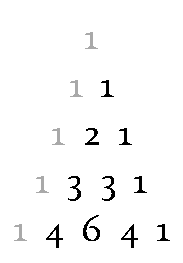
\includegraphics[width=\marginparwidth]{figs/pascal-triangle}
\caption[Pascal's triangle]{The $(i-2)$-th row of Pascal's triangle, which is obtained by adding the numbers in the row above, gives the number of faces of every dimension in an $i$-simplex. For instance, a tetrahedron (3-simplex) has 4 vertices, 6 edges, 4 faces and 1 volume.}
\label{fig:pascal-triangle}
}
This means that in a 2D simplicial complex, \ie\ a triangulation\footnote{even if it is embedded in a dimension higher than two, \eg\ the triangulated surfaces embedded in 3D (TINs) that are common in GIS}, every triangle has three vertices and three edges, and it is adjacent to at most three other triangles.
Similarly, in a 3D simplicial complex, \ie\ a tetrahedralisation, every tetrahedron has four vertices, six edges and four faces, and it is adjacent to at most four other tetrahedra.

Because of this, 2D simplicial complexes are usually stored using triangle-based data structures and 3D simplicial complexes using tetrahedron-based data structures.
These respectively use triangles/tetrahedra as primitives, which can store attributes for themselves (\eg\ whether it is part of a given object) and for (some of) their faces, and are linked to their adjacent triangles/tetrahedra.
As shown in \reffig{fig:2-simplex}, minimal representation of this type would only consist of triangles/tetrahedra linked to their vertices, either as tuples of coordinates or as separate primitives.
\begin{figure}[tbp]
\centering
\subfloat[Adjacent triangles]{
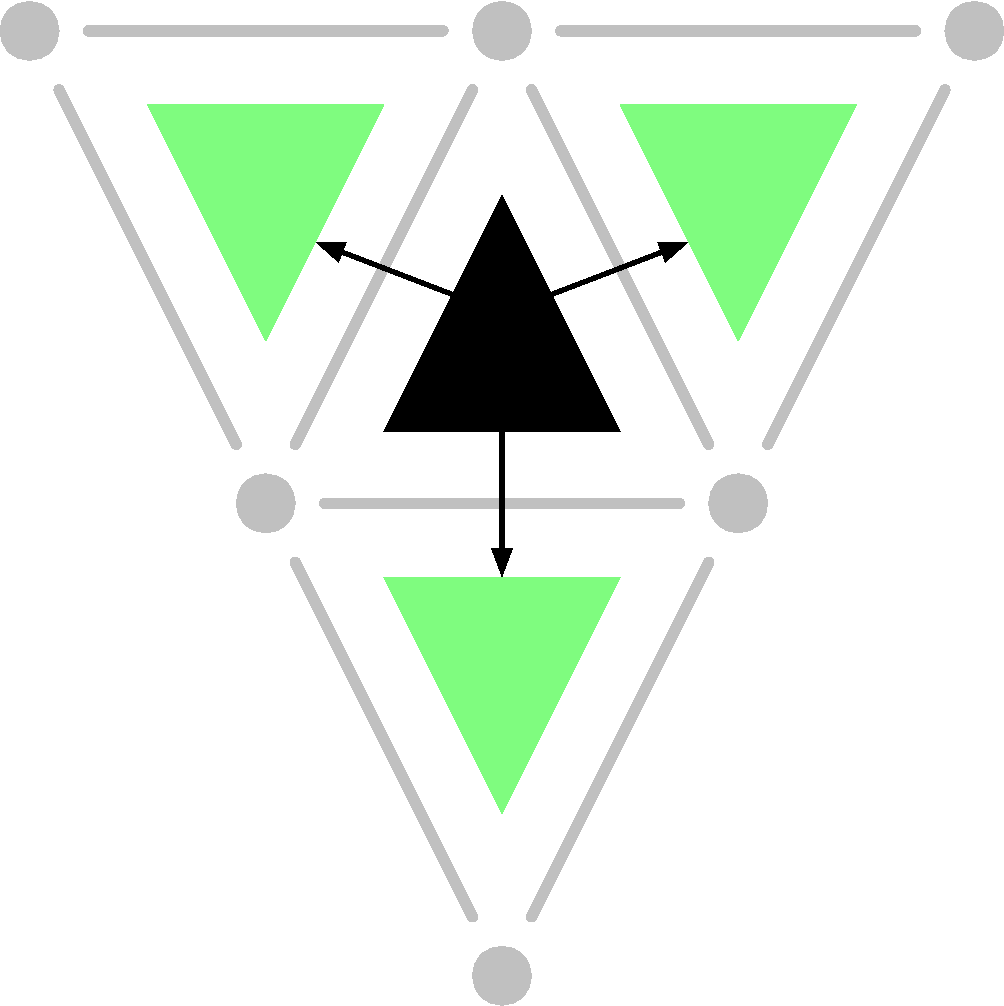
\includegraphics[width=0.27\linewidth]{figs/2-simplex-adjacency}
\label{subfig:2-simplex-adjacency}}
\quad
\subfloat[Vertices of a triangle]{
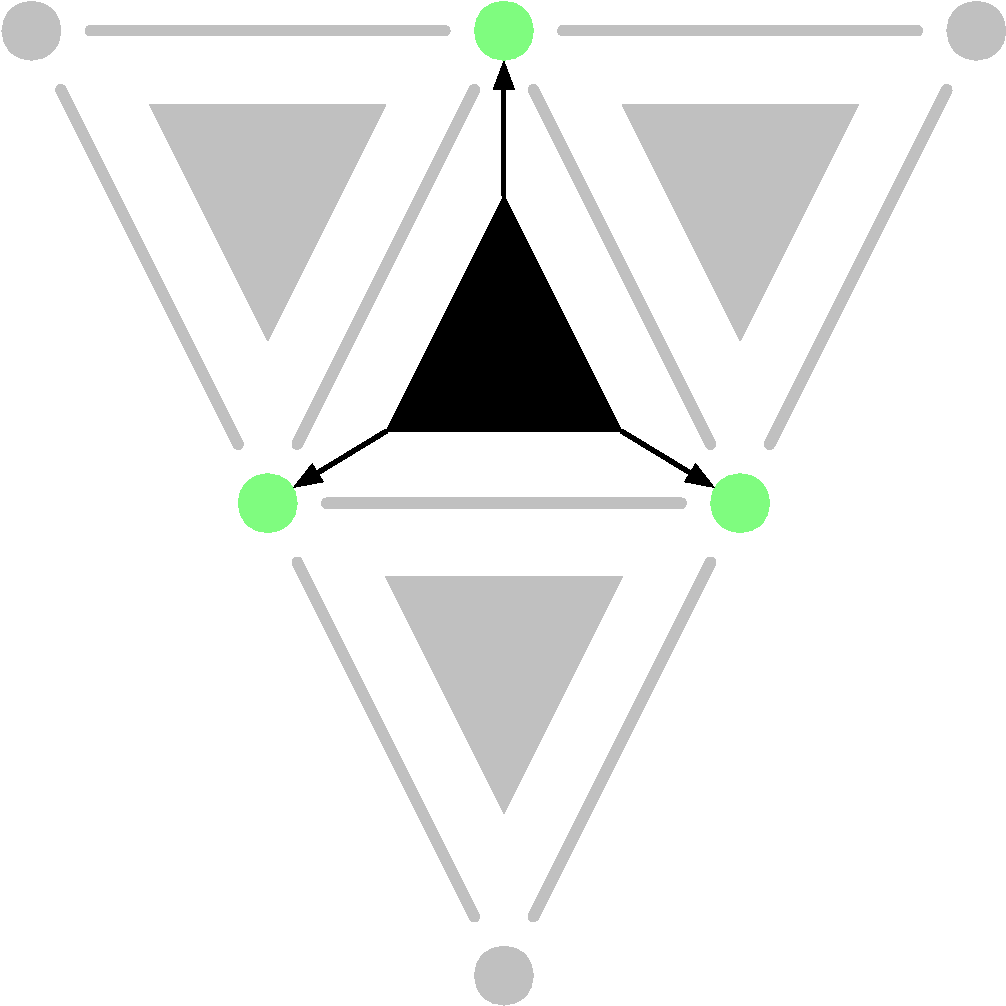
\includegraphics[width=0.27\linewidth]{figs/2-simplex-vertices}
\label{subfig:2-simplex-vertices}}
\quad
\subfloat[Coordinates of a vertex]{
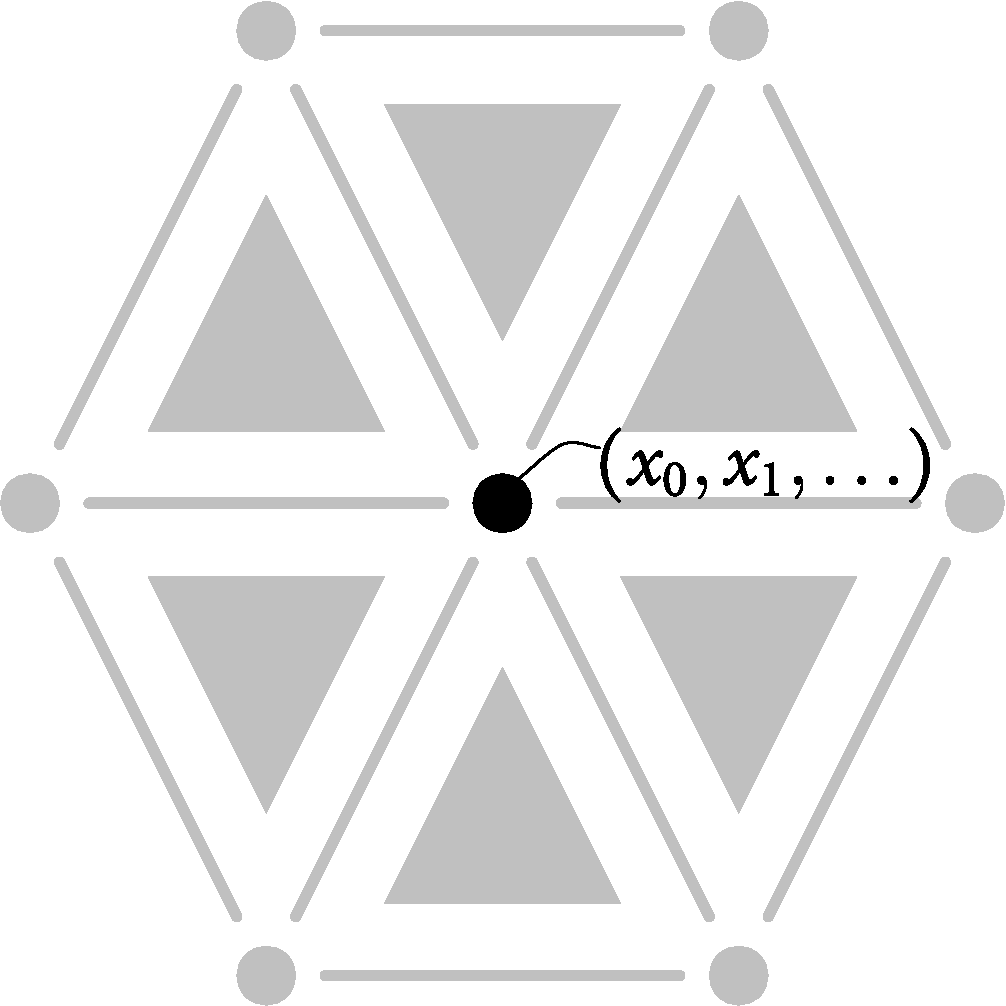
\includegraphics[width=0.27\linewidth]{figs/0-simplex}
\label{subfig:0-simplex}}
\caption[A triangle-based data structure]{A simple triangle-based data structure that consists of a set of triangles pointing to their three adjacent triangles, their three incident vertices, and a set of vertices with their coordinates}
\label{fig:2-simplex}
\end{figure}

Another possibility, also enabled by the fixed form of the simplices in a simplicial complex, is to use compression schemes in order to store them more efficiently.
For example, \citet{Blandford05} shows how several of these schemes can be used: storing only some of the vertices in each simplex, difference coding to minimise the size of the IDs that are stored, and using collections of adjacent simplices (\eg\ the star of a vertex) as primitives.
It is also possible to use progressive representations that approximate the simplicial complex incrementally~\citep{Popovic97}, or to compress it as a sequence of operations from which the original structure can be incrementally deduced \citep{Rossignac99}.

\subsubsection{2D cell complexes}

Considering the Jordan curve theorem \citep{Jordan87} and the principles of boundary representation, as presented in \refse{ss:data-models}, $n$D cells can be represented based on their ($n-1$)D boundary.
2D cells can be thus be represented based on their 1D boundary.
Since linear 1D objects, such as the polygonal curve (polyline) in \reffig{fig:polyline}, are notably easy to represent, this is the approach that is favoured by most data structures for 2D cell complexes.
\marginpar{
\captionsetup{type=figure}
\centering
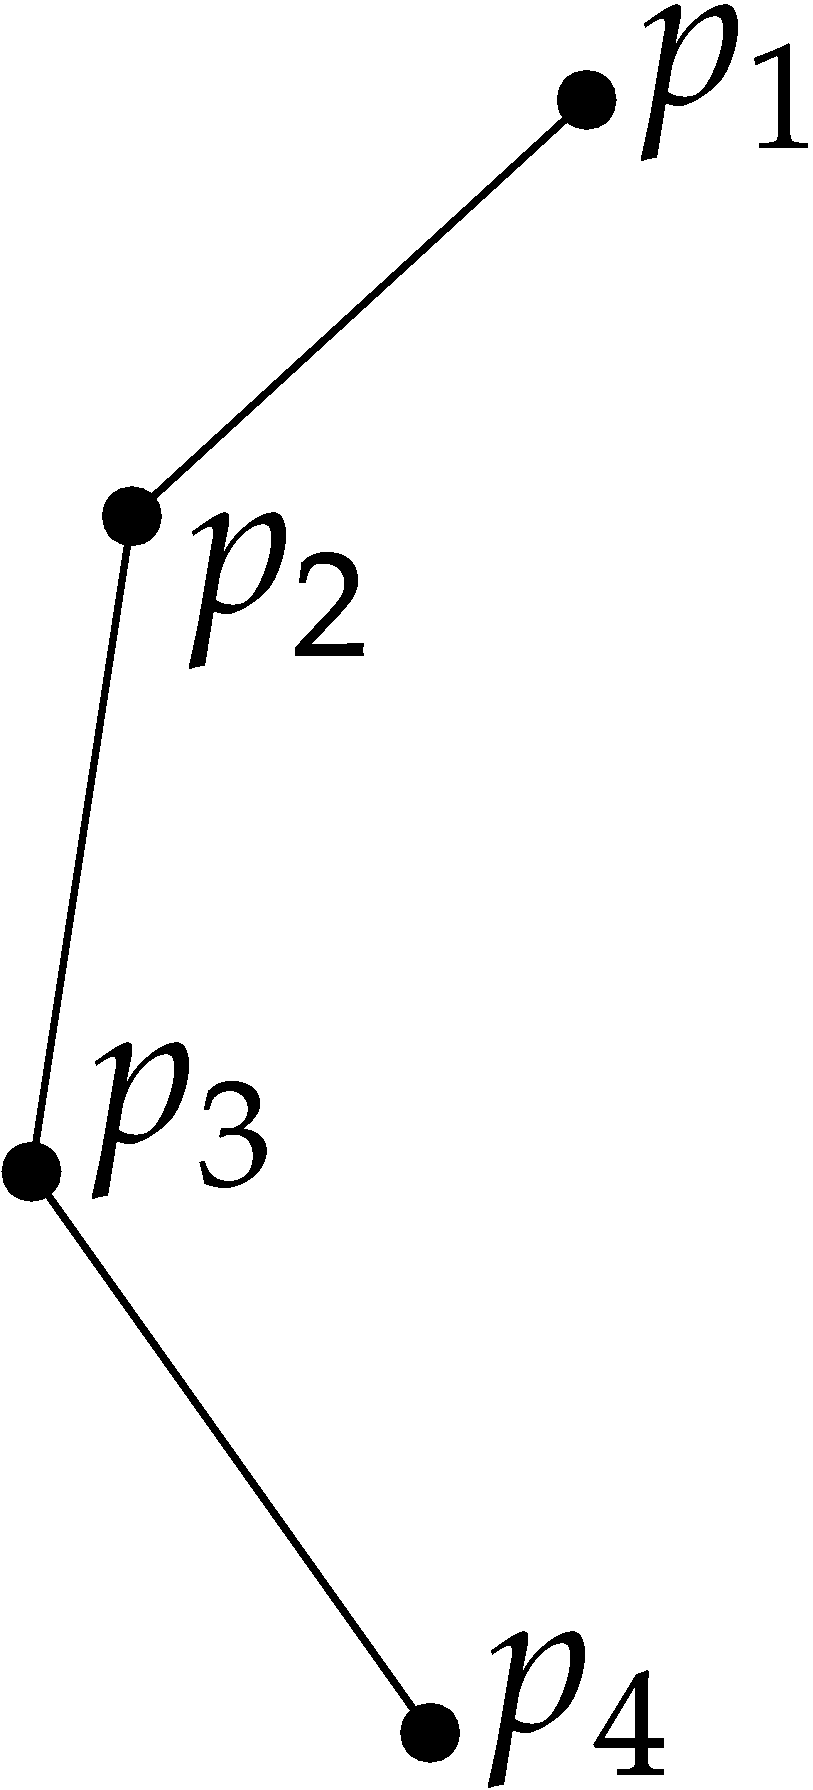
\includegraphics[width=0.5\marginparwidth]{figs/polyline}
\caption[A polygonal curve]{A polygonal curve, also known as a polyline, is a curve made from contiguous line segments. It is commonly represented as a sequence of points connected by implicit line segments, in this case $(p_1,p_2,p_3,p_4)$.}
\label{fig:polyline}
}

The simplest data structures for 2D cell complexes store every 2-cell independently as a list of vertices, as is shown in \reffig{fig:polygon-model}.
\marginpar{
\captionsetup{type=figure}
\centering
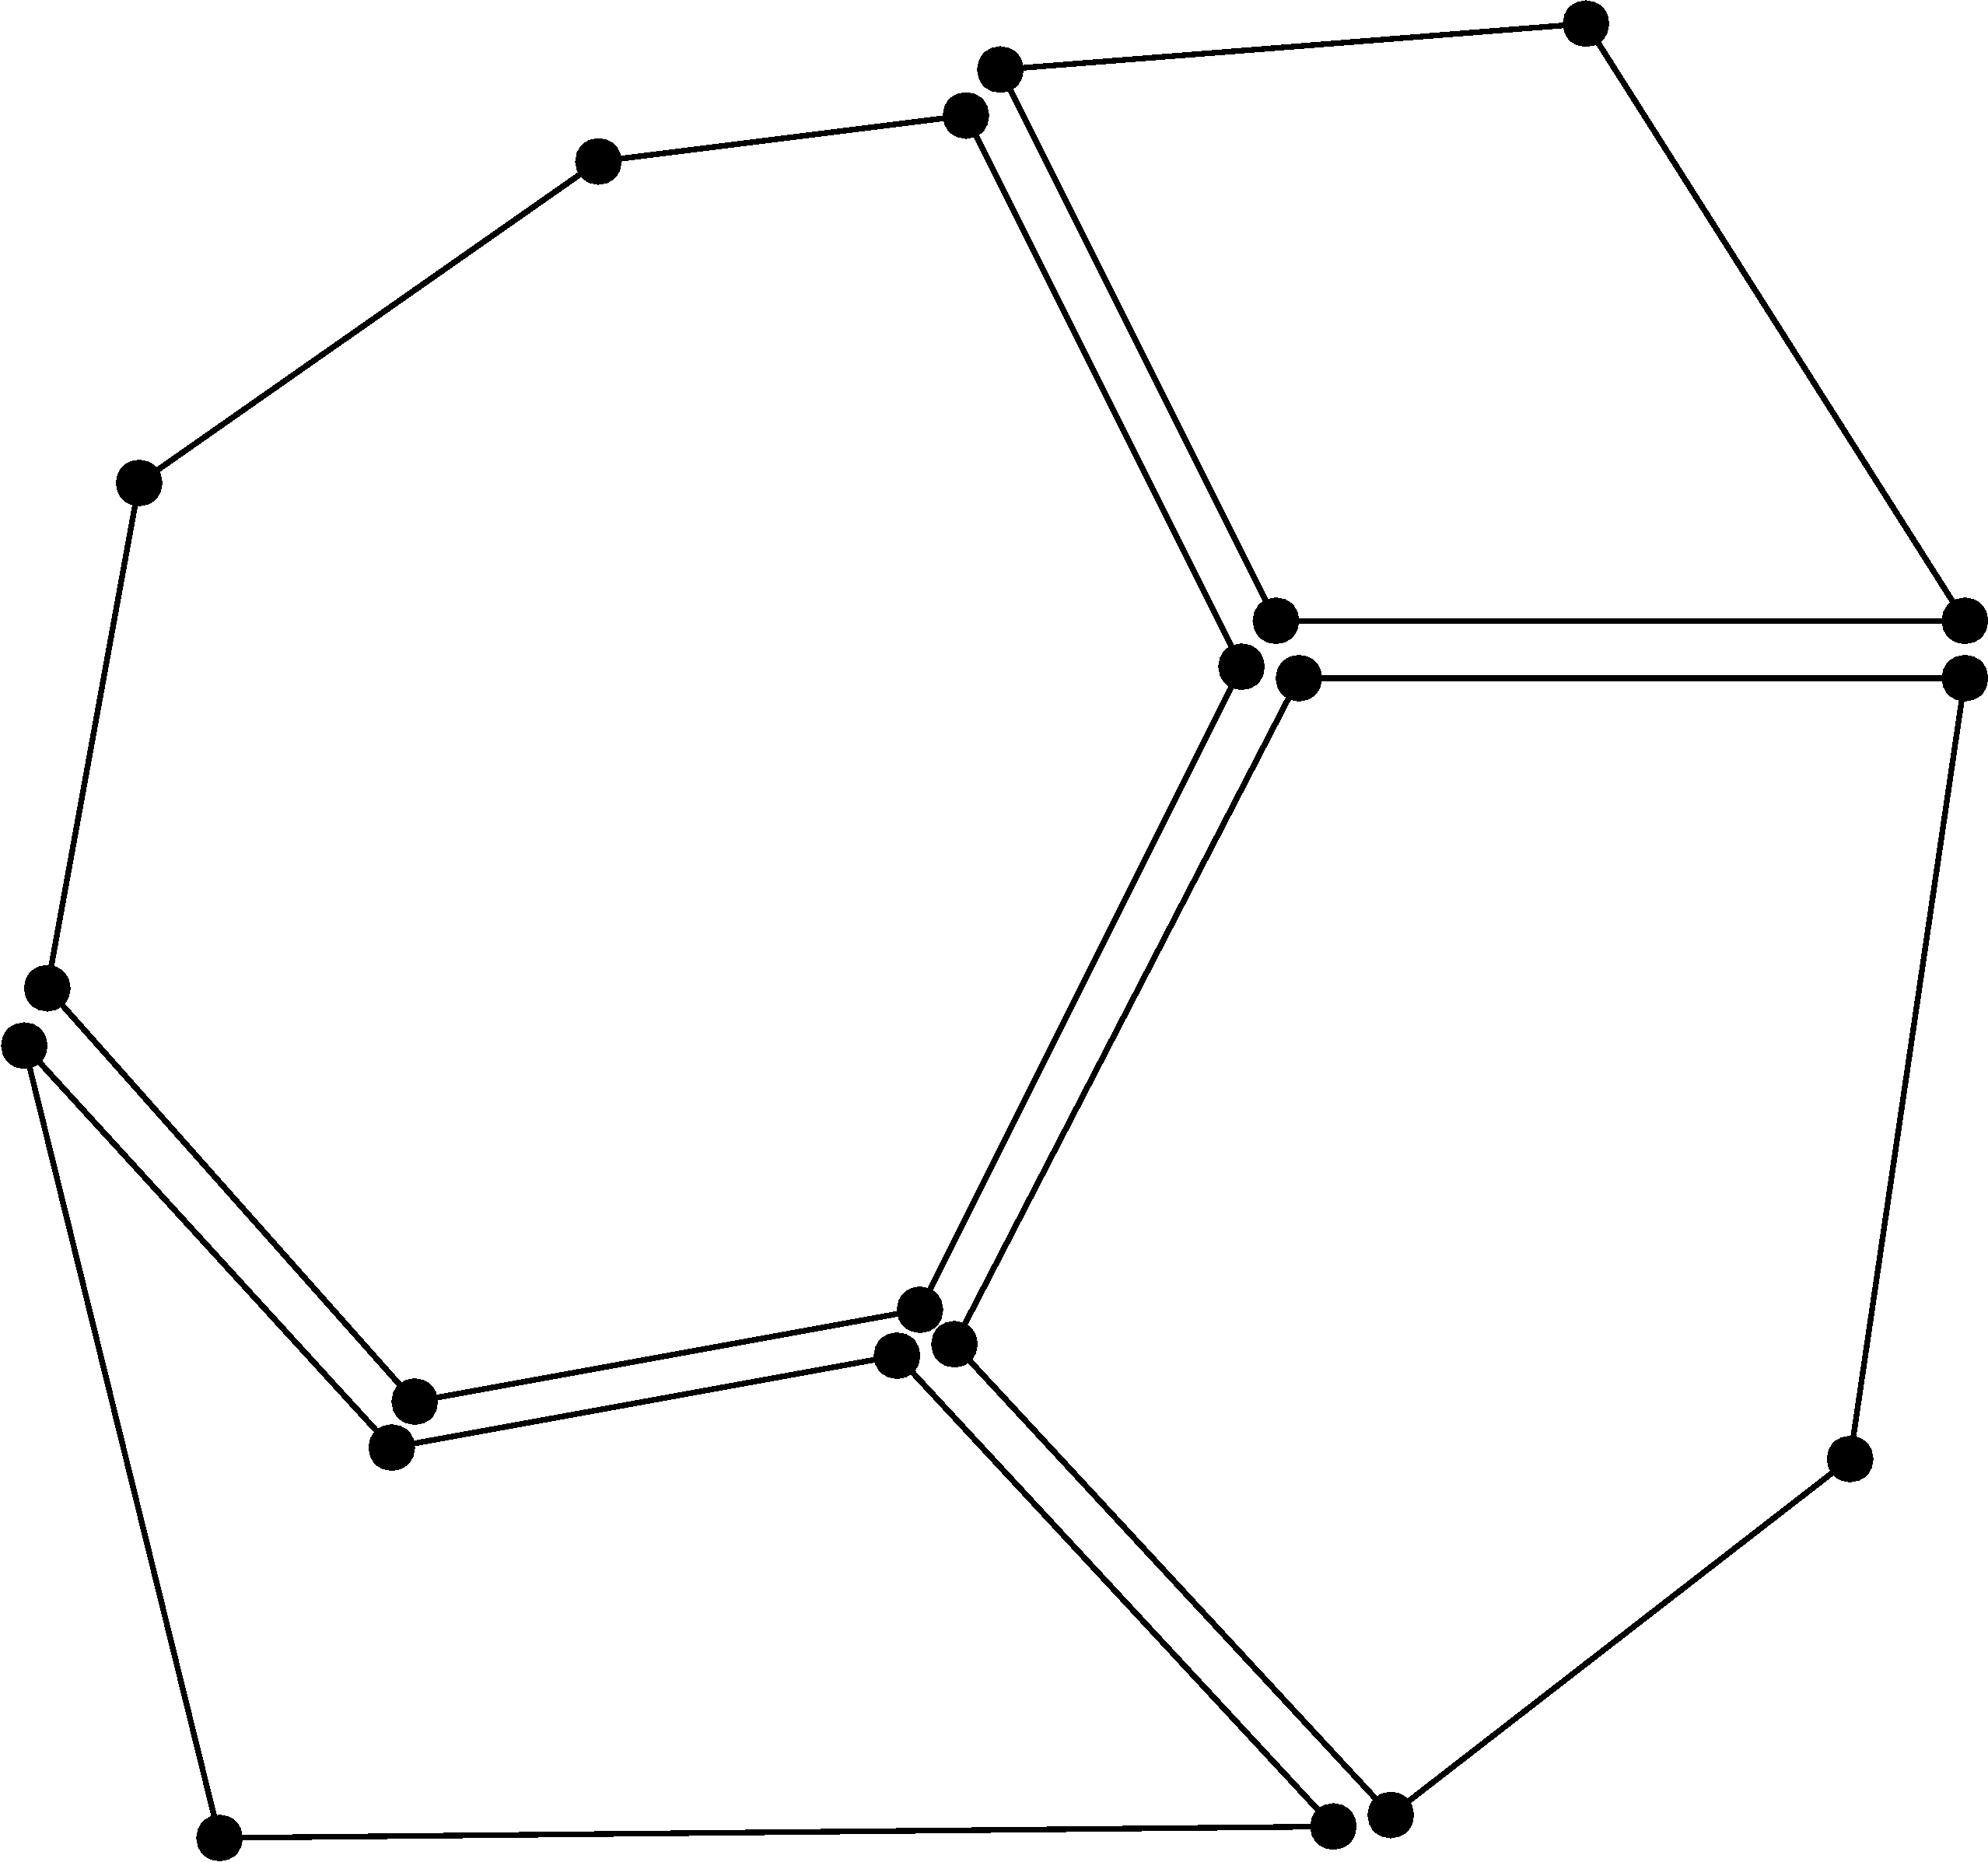
\includegraphics[width=\marginparwidth]{figs/polygon-model}
\caption[The polygon model]{In the polygon model, every polygon is represented separately as a list of vertices. Note that every vertex is thus represented once for each polygon where it is used.}
\label{fig:polygon-model}
}
This might be done by storing its coordinates directly in the list, sometimes known as the polygon model, or by keeping an external list of points and referring to point IDs in it, sometimes known as the point dictionary representation \citep{Peucker75}.

Another simple approach consists of identifying the polygonal curves that form the common boundary that lies between two polygons (or one polygon and the exterior), splitting them at the vertices that are incident to three or more polygons (or two polygons and the exterior) and storing them \emph{only once}, as is shown in \reffig{fig:spaghetti}.
\marginpar{
\captionsetup{type=figure}
\centering
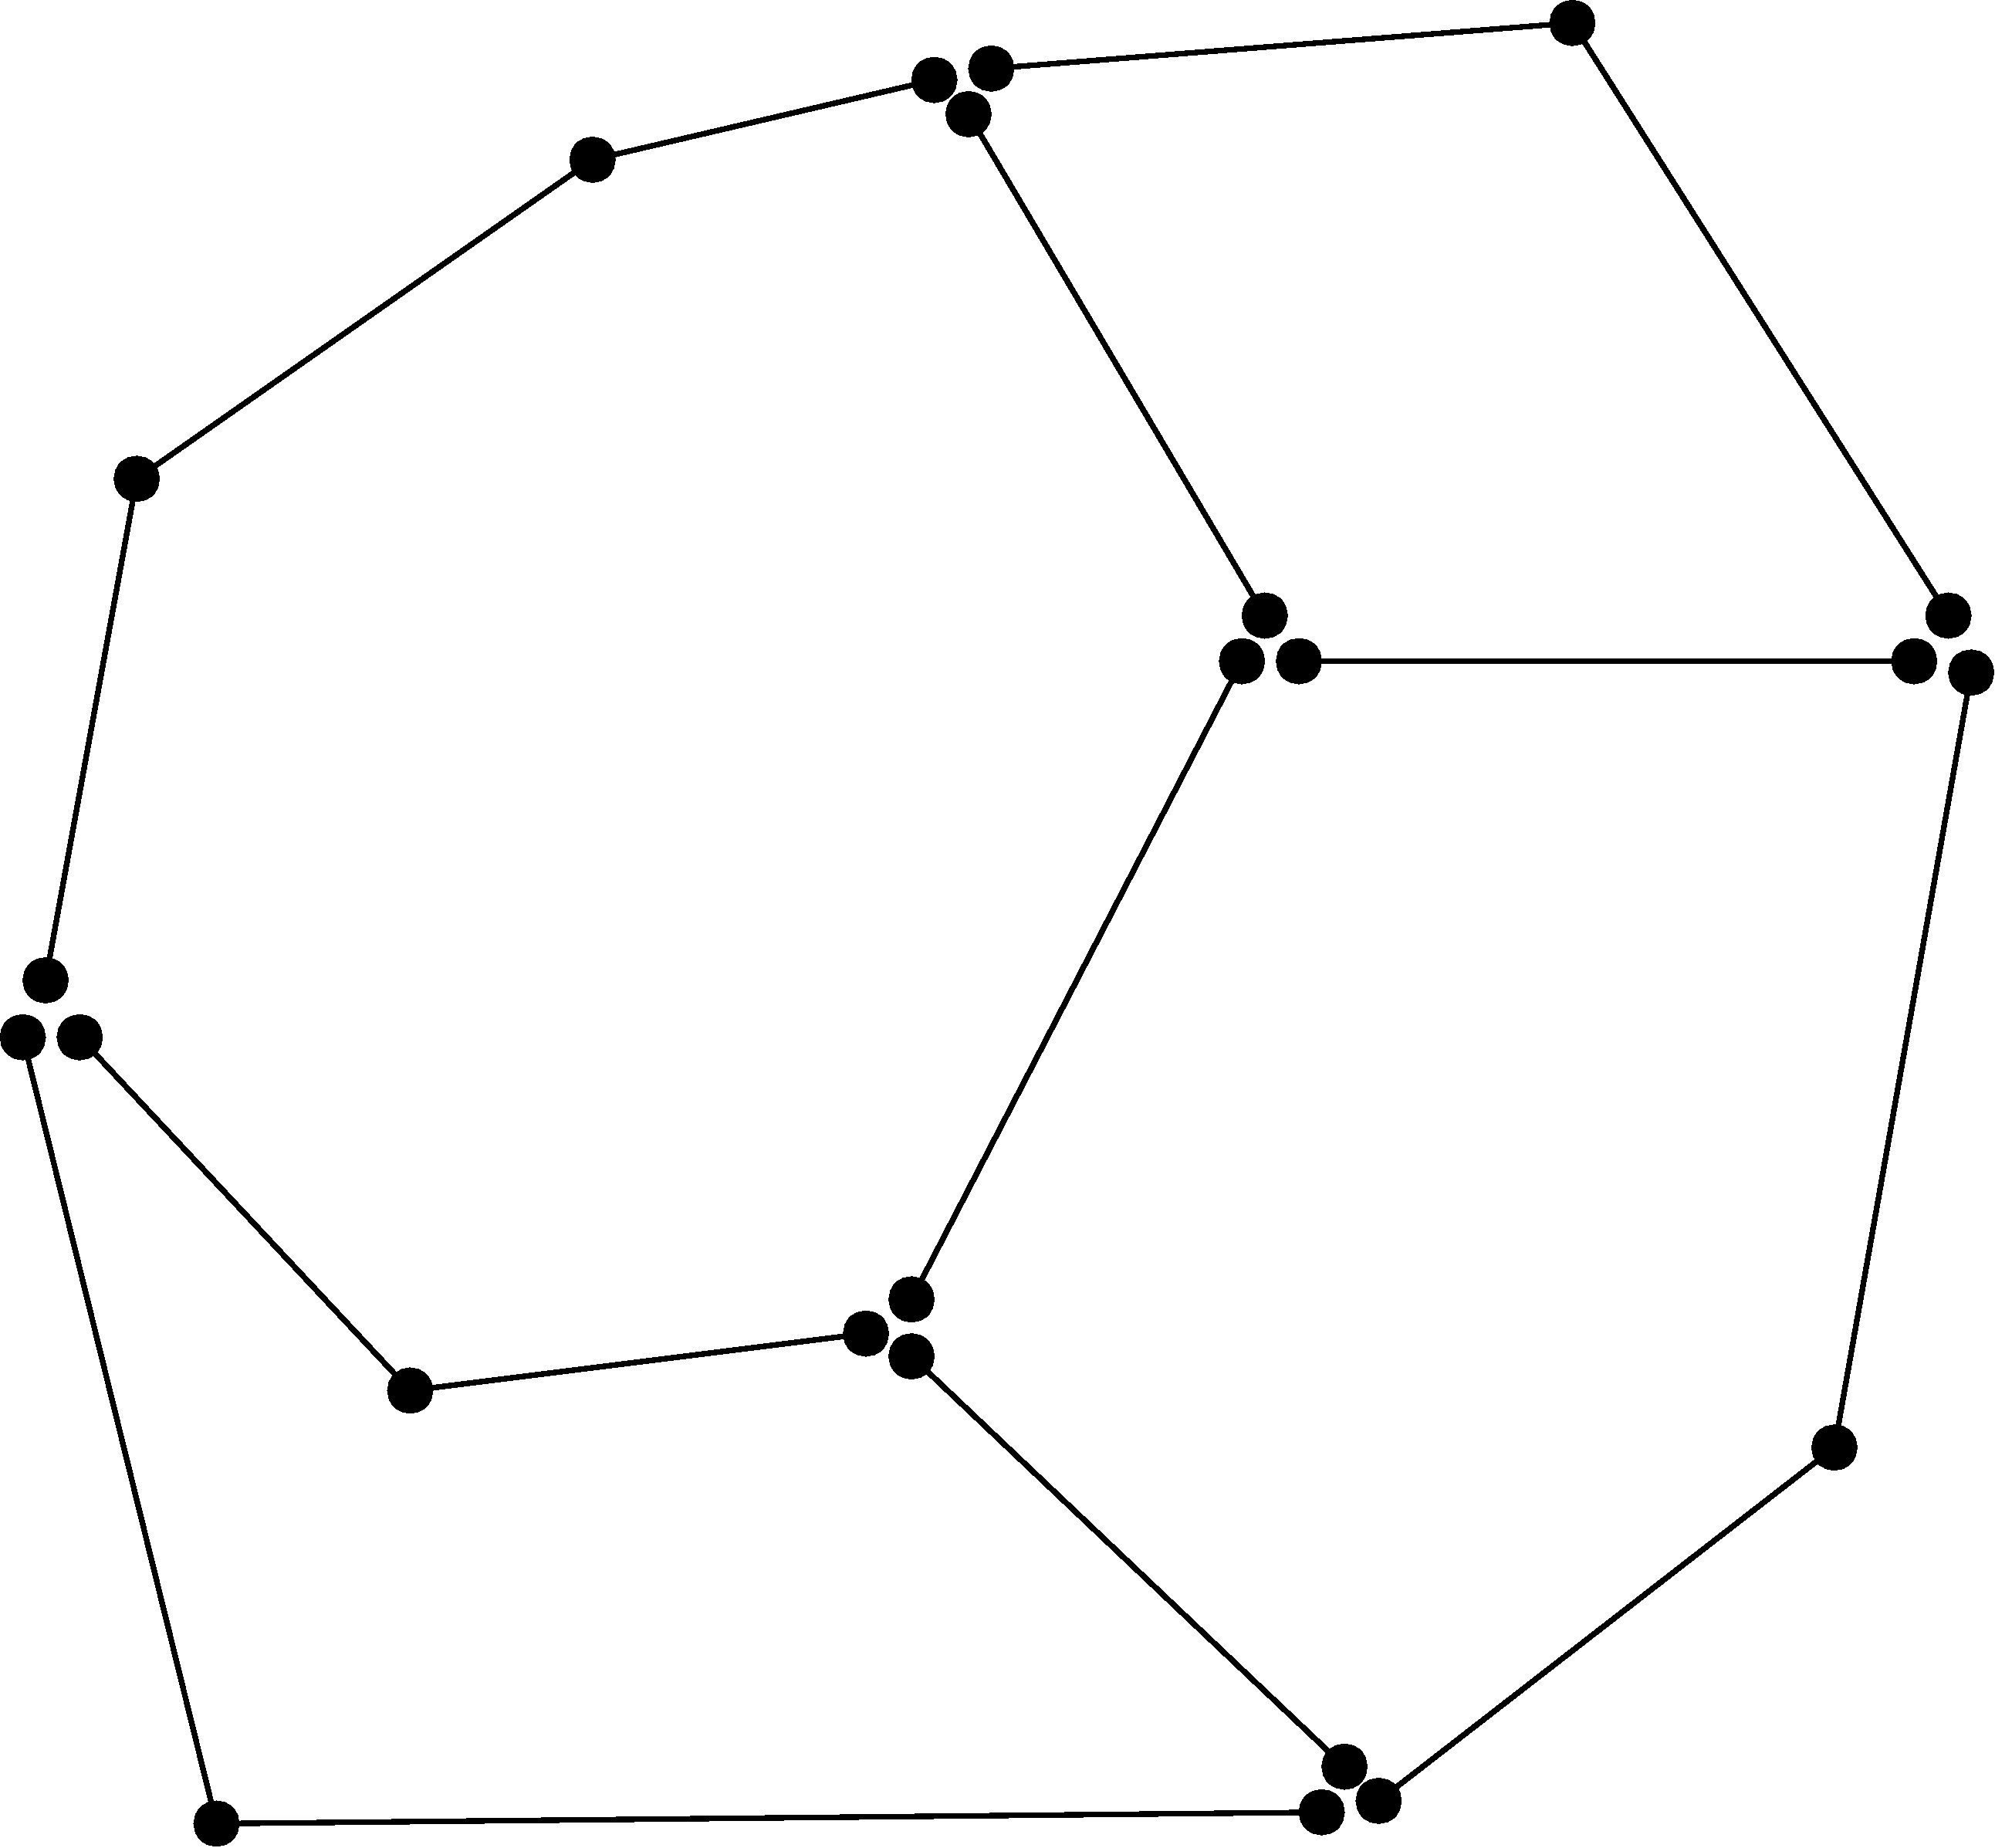
\includegraphics[width=\marginparwidth]{figs/spaghetti}
\caption[The spaghetti model]{In the spaghetti model, common boundaries are identified and represented only once. However, the polygons are only implicitly described.}
\label{fig:spaghetti}
}
This means that most points are only stored once as well (except for those at the beginning or end of these polygonal curves).
In GIS, this is sometimes known as the \emph{spaghetti model} and the polygonal curves are known as \emph{chains}\footnote{Note however that the spaghetti model can refer to other types of models. The only thing that all references to a spaghetti model have in common is the fact that chains are stored individually.}.
Unlike 3D wireframe models, these polygonal curves are sufficient to identify the polygons in a 2D cell complex\footnote{As long as it strictly conforms to the definition of a cell complex, \eg\ by having no overlapping polygons and ensuring that polygons are perfectly closed with no overshoots or undershoots.}---a problem known as polygonisation in GIS, which is related to problems with arrangements of lines in computational geometry \citep[Ch.~8]{deBerg08}.
However, additional processing is required to do so as the polygons are not stored directly.

Most other data structures take into account the fact that every edge or chain in a 2D cell complex lies between two cells, and so it is very convenient to use these edges to store information about the two cells that are incident to them.
For instance, the Node-arc-area (NAA) or POLYVRT (Polygon Converter) data structure \citep{Peucker75} also uses chains, but stores for each chain the polygons on the left and right side according to the order in which its vertices are stored.

There are several data structures based on half-edges, oriented edges or vertex-edge pairs.
All of these are functionality equivalent and are able to store a 2D cell complex or its dual.
However, since cells in a cell complex are supposed to be manifold, special care is usually necessary to represent cells with a non-manifold domain.
An example of this shown in \reffig{fig:nonmanifold-012}.
\begin{figure}[b]
\centering
\subfloat[]{
\includegraphics[width=0.29\linewidth]{figs/nonmanifold-0}
\label{subfig:nonmanifold-0}}
\quad
\subfloat[]{
\includegraphics[width=0.29\linewidth]{figs/nonmanifold-1}
\label{subfig:nonmanifold-1}}
\quad
\subfloat[]{
\includegraphics[width=0.29\linewidth]{figs/nonmanifold-2}
\label{subfig:nonmanifold-2}}
\caption[Storing non-manifold polygons in a half-edge data structure]{(a) A polygon is non-2-manifold as the space around the vertex (highlighted in a circle) is not homeomorphic to the plane (\ie\ $\mathbb{R}^2$).
Its linear boundary is non-1-manifold as the space around the vertex is also not homeomorphic to the line (\ie\ $\mathbb{R}$).
(b) \& (c) However, it can still be represented using a loop of oriented half-edges by having a duplicate vertex at that location (shown as two half balls), but there are two ways in which it can be done.
Note that these are not equally desirable as (c) results in a disconnected graph.}
\label{fig:nonmanifold-012}
\end{figure}

Among the half-edge based data structures, the winged-edge data structure \citep{Baumgart75} considers edges as the main primitive, gives them an orientation, and maintains two records for the left and right polygons, as well as four records for the previous and next oriented edges on both of these polygons.
As shown in \reffig{fig:halfedge}, the doubly-connected edge list (DCEL) \citep{Muller78} and 2D combinatorial maps \citep{Edmonds60}, achieve a similar result but have a more elegant and usually more efficient approach, dividing edges into half-edges\footnote{In the case of the DCEL this is done lengthwise, graphically resulting in side-by-side edges with opposite orientations on either side of the edge. In the case of 2D combinatorial maps it is done at the half-way point, graphically resulting in end-to-end edges. However, these are functionally equivalent.}, which allows to easily follow the cycles representing polygons.
\begin{figure}[tbp]
\centering
\subfloat[]{
\includegraphics[width=0.29\linewidth]{figs/halfedge-1}
\label{subfig:halfedge-1}}
\quad
\subfloat[]{
\includegraphics[width=0.29\linewidth]{figs/halfedge-2}
\label{subfig:halfedge-2}}
\quad
\subfloat[]{
\includegraphics[width=0.29\linewidth]{figs/halfedge-3}
\label{subfig:halfedge-3}}
\caption[A 2D cell complex as a DCEL and a 2D combinatorial map]{(a) A 2D cell complex of 3 polygons is represented using (b) the DCEL and (c) a 2D combinatorial map. In the DCEL, a half-edge $e$ is related to two vertices (the origin and the destination) and one face, and is linked to the next half-edge and a twin half-edge. In a 2D combinatorial map, a half-edge $e$ is related to one vertex and two faces (on either side), and is linked to the half-edge on the opposite side of the same edge $\alpha(e)$ and the one on the same vertex but on the next edge (as given by a rotation direction).}
\label{fig:halfedge}
\end{figure}

The quad-edge data structure \citep{Guibas85} attempts to unify most of these by rigorously naming the possible relationships between an oriented edge and other nearby oriented edges or vertices in its \emph{quad-edge algebra}, which moreover includes the dual vertices and edges of the 2D cell complex.
% These relationships are shown in \reffig{fig:quad-edge-algebra}.
% TODO: If not used later when talking about operations, remove quad-edge algebra
% \begin{figure}[tbp]
% \centering
% \subfloat[]{
% \includegraphics[width=\marginparwidth]{figs/quad-edge-algebra-1}
% \label{subfig:quad-edge-algebra-1}}
% \quad
% \subfloat[]{
% \includegraphics[width=\marginparwidth]{figs/quad-edge-algebra-2}
% \label{subfig:quad-edge-algebra-2}}
% \caption[The quad-edge algebra]{The quad-edge algebra of \citet{Guibas85} defines a large number of possible relations between an oriented edge $e$ and other oriented edges.
% These can be used to define alternative quad-edge data structures that also contain the necessary information about a map.
% Note that the grey oriented edges $eFlip$ and $eFlipSym$ lie on the back of the map.}
% \label{fig:quad-edge-algebra}
% \end{figure}
Not all of these need to be however stored.
In fact, \citet{Guibas85} proposes a structure of \emph{quads}, which store for a given edge only the previous and next oriented edges for the polygons on both of its sides.
\marginpar{
\captionsetup{type=figure}
\includegraphics[width=\marginparwidth]{figs/quad}
\caption[The quad-edge data structure]{In the quad-edge data structure, an edge stores a \emph{quad}, four records pointing to other quads corresponding to the previous and next oriented edges for the polygons on both of its sides.}
% (\ie\ $eLprev$, $eLnext$, $eRprev$ and $eRnext$ in the quad-edge algebra).}
\label{fig:quad}
}
As shown in \reffig{fig:quad}, these quads store all the necessary relationships to traverse the edges of a polygon in clockwise or anticlockwise order, as well as to navigate between adjacent polygons that are incident to a given edge or vertex.

\subsubsection{3D cell complexes}

While data structures for 2D cell complexes can rely on the fact that an edge is incident to at most two faces, this is not the case in a 3D cell complex.
The data structures for 3D cell complexes are therefore significantly more complex, requiring additional information in order to efficiently traverse the many faces incident to an edge and between different volumes.

The facet-edge data structure \citep{Dobkin87}, shown in \reffig{fig:facet-edge}, considers an incident face-edge pair as a single primitive, which is known as a \emph{facet-edge}.
\begin{figure}[tbp]
\centering
\subfloat[]{
\includegraphics[width=0.3\linewidth]{figs/facet-edge}
\label{subfig:facet-edge}}
\quad
\subfloat[]{
\includegraphics[width=0.6\linewidth]{figs/facet-edge-ops}
\label{subfig:facet-edge-ops}}
\caption[The facet-edge data structure]{(a) The facet-edge data structure considers an incident face $f_0$ and edge $e_0$ as a single facet-edge primitive $a$, each with a predefined orientation. The orientation of the face of $a$ defines the order along its incident edges $e_0,e_1,e_2,e_3$. The orientation of the edge of $a$ defines the order along its incident faces $f_0,f_1,f_2$. (b) A set of operations on the facet-edge $a$ is used to traverse the structure.}
\label{fig:facet-edge}
\end{figure}
Groups of eight of these primitives are then stored as a single group, consisting of the four different orientation combinations of a facet-edge and the ones of its dual (consisting of the dual face and dual edge of the facet-edge).

The V-map data structure \citep{Lienhardt88}, related to the notion of 2D combinatorial maps \citep{Edmonds60,Cori75}, splits edges into half-edges per edge, per face and per volume.
These half-edges, called \emph{threads}, result in faces that are modelled as cycles of half-edges, as is shown in \reffig{fig:vmap}.
\begin{figure}[tbp]
\centering
\subfloat[Tetrahedral 3-cell]{
\includegraphics[width=0.3\linewidth]{figs/vmap-1}
\label{subfig:vmap-1}}
\quad
\subfloat[V-map]{
\includegraphics[width=0.3\linewidth]{figs/vmap-2}
\label{subfig:vmap-2}}
\caption[A V-map]{A tetrahedral 3-cell is represented as a V-map. Since a V-map considers half-edges to be distinct per face and per volume, every edge is here represented by four threads. Within a face, it is possible to switch between the threads of an edge (in French \emph{ar\^ete}) with the operator $\alpha$ and between the threads of a vertex (in French \emph{sommet}) with the operator $\sigma$. In addition, it is possible to navigate between the threads on different faces or volumes with the operator $\gamma$.}
\label{fig:vmap}
\end{figure}

The radial edge data structure \citep{Weiler88} follows a similar approach, dividing faces into \emph{face uses} per volume and representing these faces uses as cycles of \emph{edge uses} where every edge use is linked to a \emph{vertex use}.
Based on this structure, it is possible to keeps a hierarchy of 3D objects, recursively composed of volumes, shells, faces, loops, edges and vertices.

\emph{Selective Nef complexes} \citep{Hachenberger06}, shown in \reffig{fig:snc}, implement 3D Nef polyhedra using a combination of two half-edge data structures, a common one that represents faces as cycles of \emph{edge-uses}, and one that represents the local pyramids around every vertex as subdivisions on the surfaces of (infinitesimally small) spheres.
This combination of data structures significantly reduces the complexity of computing certain operations on Nef polyhedra.
\begin{figure}[tbp]
\includegraphics[width=\linewidth]{figs/snc}
\caption[A selective Nef complex]{A selective Nef complex. The half-edge structure on $\mathbb{R}^3$ uses standard (oriented) faces, edges and vertices. The half-edge structure on the surfaces of the spheres uses \emph{sfaces} (not shown here), \emph{sedges} and \emph{svertices}. Note how sedges are the intersections of a face with the spheres of its incident vertices, and svertices are the intersections of an edge with the spheres of its incident (origin and destination) vertices. From \citet{Hachenberger06}.}
\label{fig:snc}
\end{figure}

\subsection{Combinatorial and embedding structures}
\label{ss:combinatorial-embedding}

In many of the data structures presented in \refse{ss:data-structures}, an additional distinction can be made between a \emph{topological} or \emph{combinatorial model} \citep{Lienhardt91}, which was the focus of the previous section and describes the connectivity between a set of predefined elements, and a \emph{geometric} or \emph{embedding model}, which specifies the exact shape and position of individual elements \citep{Mantyla88}.
This embedding model can be as simple as a point in $\mathbb{R}^3$ that is assigned to every vertex, resulting in linear geometries when the points for a face are coplanar.

However, it is often useful to have more powerful embedding information---allowing for more complex shapes (\eg\ curved surfaces) or the storage of attributes.
Normally, this embedding information is put into \emph{embedding structures} that correspond to simplices or cells and can be used to store geometric and attribute information for themselves and their faces.
When a simplex/cell has an explicit representation as a \emph{single} data structure primitive, these structures are not necessary and the information for the simplex/cell can be put into the corresponding primitive.
Otherwise, the embedding structures are separate data structures that are linked to related primitives, \eg\ the two half-edges of an edge being linked to an embedding structure containing information about the edge, or a half-edge being linked to the structures for its incident faces.

Embedding structures are also used in order to keep semantic information.
While the structures that are required for complex semantics are outside the scope of this thesis, embedding structures can store a cell's attributes as a tuple of fields for a cell.
When more complex information is required, external data structures can be kept and linked to/from the embedding structure \citep{Kuhn05}.

The geometric information that is necessary to store more complex shapes (\eg\ curves and curved surfaces) can be similarly kept as a tuple of parameters.
For instance, composite B\'ezier curves and surfaces \citep{Bezier77} can be stored using a cell complex where the vertices store \emph{control points}.
These are accompanied with some external knowledge such as the order of the curve/surface.
Non-uniform rational basis splines (NURBS) curves and surfaces \citep{Versprille75} can also be stored as a cell complex of control points with knot vectors stored as lists in the embedding structures used for the edges.

\section{Modelling of 2D and 3D space in practice}
\label{se:modelling-space}

Based on the concepts of the different data models, data structures and combinatorial/embedding structures presented above, this section discusses how these are applied and combined in practice in various international standards, file formats and software.
These are ordered from the simple geometric models that allow only for visualisation and simple calculations, up to the complex, more topological models that enable simulations and other complex computations.

\subsection{Models used in visualisation, computer graphics and gaming}
\label{ss:graphics}

The simplest geometric models are those that are used solely for visualisation.
Low-level application programming interfaces (APIs) for 3D graphics, \eg\ OpenGL\footnote{\url{https://www.opengl.org}}, Direct3D\footnote{a subset of DirectX:\ \url{http://msdn.microsoft.com/directx}}, Mantle\footnote{\url{http://www.amd.com/mantle}}, WebGL\footnote{\url{https://www.khronos.org/webgl/}} and Vulkan\footnote{\url{https://www.khronos.org/vulkan/}} work with large numbers of simple geometric primitives with 3D coordinates, such as points, line segments and triangles, all of which can be used alone or as structured sequences (such as the triangle strip in \reffig{fig:trianglestrip}).
\marginpar{
\captionsetup{type=figure}
\centering
\includegraphics[width=0.7\marginparwidth]{figs/trianglestrip}
\caption[A triangle strip]{A triangle strip is easily defined as a list of vertices $(a,b,c,d,e,f,g,h)$. Every triangle is formed by three consecutive vertices in the list.}
\label{fig:trianglestrip}
}
These can be passed directly, loaded into video memory, and be processed and rendered in parallel by graphics hardware.
Subproblems in this process are therefore offloaded onto techniques that can be easily parallelised and done in hardware.
For example, the visibility computations involved when rendering a set of polygons in 3D can be handled using Z-buffers \citep{Strasser74}.

\subsection{Exchange file formats and standards in GIS and BIM}
\label{ss:formats}

The file formats that are meant for the exchange of spatial objects in GIS---sometimes codified in (international) standards---generally opt for a minimal representation of the geometries involved.
Polylines and polygons are thus stored as sequences of points connected by implicit line segments, as this is a more compact and intuitive representation than a set of (unordered) line segments.
By contrast, volumes are represented as (unordered) sets of their bounding polygonal faces.
As no topological relationships are recorded between these polygons, these types of representations are known as \emph{non-topological models} in GIS.\@

\begin{figure*}[tbp]
	\begin{center}
		\includegraphics[width=\linewidth]{figs/sfs}
	\end{center}
	\caption[Geometry in the Simple Features Specification]{The geometry class hierarchy defined in the Simple Features Specification \citep{SimpleFeatures1}.}
\label{fig:sfs}
\end{figure*}

The Simple Features Specification \citep{SimpleFeatures1} is an international standard from both the Open Geospatial Consortium and the International Organization for Standardization (as ISO 19125 \citep{ISO19125-1:2006}).
It is widely used as the basic geometric model in simple GIS formats and defines a variety of geometry classes, each of which is linked to a reference system.
These are shown in \reffig{fig:sfs}.
A \texttt{LineString} (or \texttt{LinearRing}) is represented as a sequence of two or more \texttt{Points}.
Apart from this relation and ignoring the generalisation relationships, the classes form a tree structure, with higher-dimensional classes being simple aggregations of lower-dimensional ones.
A \texttt{Polygon} is made of at least one \texttt{LinearRing} (one outer and possibly multiple inner ones defining holes), and a \texttt{PolyhedralSurface} is made of a set of patches of \texttt{Polygons}.
No relationships connect a class with itself or others of the same dimension.

\begin{figure}[t]
  \begin{center}
    \includegraphics[width=\linewidth]{figs/gml}
  \end{center}
  \caption[Geometry in GML]{The geometric classes from the ISO 19107 standard \citep{ISO19107:2005} that are implemented in the GML standard \citep{GML3.2.1}.}
\label{fig:gml}
\end{figure}

GML \citep{GML3.3}, is the most widely used international standard to represent 2D and 3D geographic information.
It has been further formalised as ISO 19136 \citep{ISO19136:2007} and is the basis of other standards, such as CityGML \citep{CityGML2} for the exchange of 3D city models.
In terms of geometry, it implements a subset of the types in the ISO 19107 standard \citep{ISO19107:2005}, which are shown in \reffig{fig:gml}.
It similarly considers \texttt{LineStrings} represented as sequences of at least two points, \texttt{LinearRings} as sequences of at least four points\footnote{There is no implicit connection between the first and last points in a CityGML polygon, so the first point needs to be repeated at the end.}.
\texttt{Polygons} consist of one exterior and zero or more interior \texttt{Rings}, and various surface types are composed of different kinds of \texttt{SurfacePatches}.

The Industry Foundation Classes (IFC)\footnote{\url{http://www.buildingsmart-tech.org/specifications/ifc-releases}} standard is an open data model used in the Building-information modelling (BIM) domain for the exchange of construction models, often including 3D models of buildings.
It has also been adapted as the ISO 16739 international standard \citep{ISO16739:2013}.
Its geometric aspects are however mostly defined or derived from a different standard---ISO 10303 \citep{ISO10303:2014}.
Unlike the data models originating in GIS (\eg\ Simple Features and CityGML), there is an important emphasis on the definition of a local coordinate system per object (as opposed to the national or regional coordinate systems used in GIS).
This reflects the fact that in BIM every object is generally modelled independently before later being fitted together.
Boundary representation and tessellation geometries are supported as in other models, but IFC supports a much greater variety of geometry classes, which include implicit geometries based on Constructive Solid Geometry (as a tree of Boolean set operations) and sweeps (based on a cross-section), such as the one shown in \reffig{fig:ifc}.

\marginpar{
\captionsetup{type=figure}
\centering
\subfloat[]{
\includegraphics[width=\marginparwidth]{figs/ifc-1}
\label{subfig:ifc-1}}
\\
\subfloat[]{
\includegraphics[width=\marginparwidth]{figs/ifc-2}
\label{subfig:ifc-2}}
\caption[Sweeps in IFC]{The IFC standard supports objects defined through sweeps, which are defined by (a) an \texttt{IfcPCurve} (black spiral) and a \texttt{SweptArea} (blue disk), in this case resulting in (b) a screw shape.}
\label{fig:ifc}
}

\subsection{Models used in 2D and 3D GIS}

When the first GIS were developed in 1960s and 1970s, such as SYMAP \citep{Chrisman88} and the Canada GIS \citep{Tomlinson88}, they used boundary representation, depicting 2D areas as polygons defined by a sequence of vertices.
By the 1980s, a \emph{topological approach} based on planar partitions was instead used in systems like GRASS\footnote{\url{http://grass.osgeo.org}} and the coverages of ArcInfo \citep{ESRITopology}.
This was done using an intermediate representation where all input objects are partitioned into homogeneous regions \citep{Rossignac89}, such that each region is linked to a set of input objects that are all present in the entire region.
This intermediate representation is obtained by performing geometric intersection operations on all of the input objects and allows these partitions to be represented using the types of data structures for 2D cell complexes presented in \refse{ss:data-structures}.

However, current 2D GIS software has reverted to the use of simple data structures with very little or no topology, which are then supplemented by external spatial indices for speed.
This type of representation has some drawbacks: it encourages inefficient representations where primitives are represented multiple times (\eg\ when a face is part of the boundary of two polyhedra) \citep[Ch.~3]{Cromley92}, which might not match exactly \citep{delaLosa99}, it makes it difficult to check that a set of bounding elements conforms to certain properties (\eg\ properly enclosing a space or being manifold), and the topological relationships between many elements need to be recomputed.

However, in the context of current 2D GIS software, in which different data sources are dynamically loaded and used together, it is often more efficient to opt for a representation with little topology, instead computing topological relationships only if and when they are needed, such as is done in ArcGIS \citep{ESRITopology} and in some QGIS plug-ins only for certain operations.
Many present use cases can actually do without the computation of these topological relationships: as explained in \refse{ss:graphics}, visualisation does not require explicit topology, today's fast computers can process many datasets using brute force approaches, and algorithms can take advantage of strong properties that are intrinsic to the 2D case, such as that it is possible to define a natural (sequential) order for the points around a closed polygonal curve, or that there can be at most two polygons incident to any edge in a planar partition.

Moreover, it is more robust---and often more convenient---to consider the geometric and topological information that is stored in a file as suspect, programming defensively to avoid errors in software by using repair techniques such as those that will be discussed in \refch{ch:cleaning}, as errors can frequently appear due to a variety of causes, \eg\ numerical errors \citep{Goldberg91,Schirra97} or differing interpretations of invalid objects \citep{Ledoux14}.

The situation regarding 3D GIS is more complex, consisting of many small ad hoc systems described in the literature (\eg\ \citep{Zhang11}) following both topological and non-topological approaches, but few general purpose publicly available 3D GIS.\@
In addition to this, there is limited 3D functionality in existing GIS software, such as 2.5D data containing elevation as an attribute \citep{Raper89}, or capabilities for simple storage, visualisation and editing (\eg\ moving vertices) of 3D models.
This leaves more complex geometric operations, such as the use of Boolean set operations or complex deformations of 3D models within the realm of CAD or 3D modelling software.
Partly as a consequence, 3D GIS datasets commonly contain large numbers of invalid geometries \citep{Zhao14}.

\subsection{Models used in 3D modelling software and libraries}

Compared to GIS software, 3D modelling, CAD and other similar software have a greater emphasis on (interactive) editing and other operations that alter the geometry of a 3D object.
However, many (or most) 3D modelling software\footnote{Unfortunately, it is difficult to know which data structures are used internally in most commercial software, so this analysis is necessarily limited.} represent 3D objects only as closed surfaces, using triangular or polygonal meshes that can be stored using the data structures for 2D simplicial/cell complexes presented in \refse{ss:data-structures}.
This is not a limitation for simple 3D editing functionality, such as moving vertices, splitting edges and faces, and adding new vertices/edges/faces.
However, more complex geometric operations with and between 3D objects generally require more powerful data structures with an explicit knowledge of volumes.

Nevertheless, some software that is used for this purpose follows a minimal approach similar to the one used for exchange file formats in GIS.\@
The standard \emph{topological data structure} in CAD\footnote{It is important to note the `topological data structure' has opposite meanings in GIS and CAD.\@
The non-topological (Simple Features) approach in GIS is equivalent to the standard CAD topological data structure; the standard GIS topological data structure is equivalent to a CAD mesh, which is widely considered as the \emph{less} topological approach. Objectively, they both embrace topology in different ways. The GIS topological data structure stores the topological relationships between polygonal areas; the CAD topological data structure stores the topological relationships between a polygon/polyhedron and its different rings/shells.} considers \emph{vertices}, curved \emph{edges} connecting vertices, \emph{wires} consisting of a closed loop of edges, \emph{faces} made from one outer wire and possibly multiple inner wires, closed \emph{shells} made from a set of faces, and \emph{solids} consisting of one outer shell and possibly multiple inner shells.
For example, this is the approach that is used in K-3D \citep{Shead10} and openCASCADE library\footnote{\url{http://www.opencascade.org}}, the engine used for geometric computations in CAD software like FreeCAD\footnote{\url{http://www.freecadweb.org}} and the SALOME numerical simulator\footnote{\url{http://www.salome-platform.org}}.

This approach often fails when attempting some operations that are notoriously difficult to perform robustly, \eg\ Boolean set operations between polyhedra---something that is recognised in the documentation of multiple software packages.
Other software thus uses more powerful data structures based on 3D cell complexes, generally achieving better results in the process.
Blender\footnote{\url{http://www.blender.org}} uses something akin to the radial edge structure \citep{Weiler88}, Moka\footnote{\url{http://moka-modeller.sourceforge.net}} uses 3D generalised maps \citep{Lienhardt94}.

A different approach is followed by software like BRL-CAD\footnote{\url{http://brlcad.org}}, which uses a Constructive Solid Geometry engine and therefore stores objects as trees of Boolean set operations.
Finally, the Nef polyhedra implementation in CGAL \citep{Hachenberger06} is able to compute Boolean set operations \citep{Granados03}, convex decompositions \citep{Chazelle84} and Minkowski sums robustly.
It is used in software like OpenSCAD\footnote{\url{http://www.openscad.org}}.

\section{Spatiotemporal modelling}
\label{se:modelling-time}

Among the possible non-spatial characteristics that can be integrated with space, time in particular has long been considered to be interlinked with space \citep{Akhundov86}.
Like space, it is considered to have geometry and topology \citep{Earman77}, which are often modelled in accordance to the ISO 19108 standard \citep{ISO19108:2002}.

Spatiotemporal modelling attempts to create joint models that combine spatial and temporal information.
It draws inspiration from the independent modelling of both space and time.
The main models used in spatiotemporal modelling are presented below.
For a more thorough review of spatiotemporal models see \citet{Al-Taha94} and \citet{Pelekis04}.

The simplest and most widespread spatiotemporal model involves the use of timestamps.
Known as the \emph{snapshot} model, it was probably first used in the US Historical Boundary File \citep{Basoglu78}.
In this model, as shown in \reffig{fig:st_snapshot} every entity represents the state of an object during a specific timeframe.
\marginpar{
\captionsetup{type=figure}
\centering
\includegraphics[width=\marginparwidth]{figs/st_snapshot1}
\includegraphics[width=\marginparwidth]{figs/st_snapshot2}
\includegraphics[width=0.6\marginparwidth]{figs/st_snapshot3}
\caption[The snapshot model]{The snapshot model stores the state of a map at various moments in time. From \citet{Langran88}.}
\label{fig:st_snapshot}
}
These entities might be objects of any dimension, \eg\ polylines as in the US Historical Boundary File or polygons in a cadastral database \citep{Hunter90}.
An entity is therefore attached with a pair of timestamps, which indicate the start and end of the period during which the object existed as is represented.
These models thus keep multiple representations of 2D \citep{Armstrong88} or 3D \citep{Hamre97} structures.
This approach is simple but not very powerful, containing no direct relations between temporal objects.

There are a few variations of this model.
For instance, it is possible to store differential changes only \citep{Langran88}, specifying the areas that are added to or removed from an object at a given time.
Another related possibility is keeping the current state of the map explicitly as well, which improves the query time.

In the \emph{space-time composite} model, objects are first split into homogeneous regions that share the same history, similar to how overlapping objects are handled in topological GIS models \citep{Rossignac89}.
This was first described in \citet{Chrisman83} based on \citet{Peucker75}.
This is more flexible than the snapshot model, but objects can become very fragmented, slowing down many operations.
For instance, updating the attributes of an object might involve updating all the regions that the object is split into.

Other models put a greater emphasis on events, such as by keeping a list of changes per object \citep{Worboys92,Peuquet94}.
Event-based models \citep{Peuquet95} take this a step further, maintaining a main structure consisting of a list of events and a base map.
\begin{figure}[tbp]
\centering
\includegraphics[width=0.85\linewidth]{figs/st_events}
\caption[An event-based model]{An event-based model maintains a list of events and a base map, with each event being linked to all changes that occurred since the last event. From \citet{Peuquet95}.}
\label{fig:st_events}
\end{figure}
Unlike other models, this makes it possible to identify and attach attributes to individual changes and events.
In the \emph{history graph} model \citep{Renolen96}, different types of events are supported, which makes it possible to model continuously changing events as well.
Similar models are used in computer animations, where a graph of keyframes can identify topological changes in a 2D vector drawing \citep{Dalstein15}.

A different option is to keep track of space and time independently, linking objects appropriately.
So called \emph{three-domain} models are based on this concept (the third domain being semantics).
Examples include \citet{Yuan94} and \citet{Claramunt95}.
\citet{vanOosterom97} uses an identifier consisting of both a region identifier and a timestamp to index spatiotemporal objects.

Finally, there are some generic spatiotemporal models described at a more conceptual level \citep{Story95}, which can be adapted to suit a specific application.
For instance, \citet{Tryfona99} describes the space-time entity-relationship model, based on the entity-relationship \citep{Chen76} common in the database world.
It provides rudimentary support for multi-scale objects by allowing for multiple geometries to be stored in each feature.
\citet{Claramunt99} discusses an object-relational model that is specifically tailored to model change.
Additionally, there are a few object-oriented spatiotemporal models \citep{Worboys90}.

\section{Modelling geographic scale}
\label{se:modelling-scale}

Traditional paper maps and physical models have a well-defined \emph{scale}, whose value is a ratio between a linear measure in the model/map with the corresponding linear measure in the real world\footnote{Non-linear measures (\eg\ area and volume) in a model/map and reality are related---appropriately---non-linearly to this ratio.}.
Scale is therefore a concept that is fixed and has a clear, measurable value in a model or map.

However, apart from this direct meaning, scale also has an indirect relation to the \emph{level of detail} (LOD) that is present in a map/model.
Considering limits in resolution in printing and manufacturing technologies, the detail that can be put into a map or model is limited by its scale.
Moreover, since humans are only able to reliably distinguish features of a certain size---a commonly accepted measure for maps being 0.5 mm \citep{Goodchild01}---, an adequate representation at a given scale presupposes objects being of a certain minimum size and a minimum distance apart.
These factors limit the detail that \emph{can} be present in a model/map at a given scale, but there are additional limits on the detail that \emph{should} be present in a map at a given scale.
Considering that maps are first and foremost communication tools, good maps need to have content of an appropriate level of precision and detail in order to convey their intended message \citep{Hardy12}.

In the digital realm, where models and maps both become data and the direct meaning of geographic scale as a ratio between a model/map and reality disappears, scale preserves only its indirect meaning as the level of detail that is present in a model or map, and accordingly the term `level of detail' is more widely used \citep{Biljecki14}.
An increase in the detail of a model enables more applications, but means that its representations occupy larger sizes and their processing involves higher computational costs.
When the term `scale' is used instead, the level of detail that is expected is often presented in relation to its physical predecessor, such as in the map fragments shown in \reffig{fig:generalisation}.
In digital models and maps, having an adequate level of detail also becomes important as a higher level of detail entails a correspondingly higher memory and computational requirements \citep{Luebke03}.
\begin{figure}[tbp]
\centering
\subfloat[1:50 000]{
\includegraphics[width=0.46\linewidth]{figs/generalisation2}
\label{ss:generalisation2}}
\quad
\subfloat[1:250 000]{
\includegraphics[width=0.46\linewidth]{figs/generalisation3}
\label{ss:generalisation3}}
\caption[Topographic maps at different scales around Delft]{Fragments of two Dutch topographic maps at different scales around Delft. Note that the region depicted in both maps is the same and maps are (here) presented at the same size, and thus the scale of both in a literal sense is the same. However, the level of detail in each map differs. \copyright\ Kadaster\protect\footnotemark.}
\label{fig:generalisation}
\end{figure}
\footnotetext{\url{http://www.kadaster.nl}}

Geographic information at different scales is generally managed as fully independent datasets at each scale \citep{Meijers11}, such as in the topographic maps shown in \reffig{fig:generalisation}.
In 3D, the CityGML standard \citep{CityGML2} defines the five LODs shown in \reffig{fig:citygml-filip}, which can be stored jointly but are effectively separate datasets except when their geometries are linked (\cf\ \citet{Biljecki15}).
This is similar to the snapshot model for spatiotemporal information \citep{Basoglu78,Langran88} as presented in \refse{se:modelling-time}, since these datasets are labelled with the scale (or range of scales) that they are associated with.
This representation is simple and matches nicely with paper map series---in which a region is depicted at multiple scales in different maps.
However, many objects are represented several times (once at each scale in which they are present) \citep{Friis-Christensen03}, and it is difficult to maintain consistency between these representations \citep{Buttenfield89}, as the different representations of an object are unlinked or linked only by common identifiers.

\begin{figure}[tbp]
\centering
\includegraphics[width=\linewidth]{figs/citygml-filip}
\caption[The LODs in CityGML]{The CityGML standard \citep{CityGML2} defines five LODs for 3D city models, which range from building footprints to detailed architectural models of their interior and exterior. From \citet{Biljecki14a}.}
\label{fig:citygml-filip}
\end{figure}
% TODO: Check Filip's citation (paper accepted?)

In order to achieve consistency and complete coverage of a region at a given scale, it becomes important to be able to create a map of that scale using a more detailed map of the same region as input, resulting in maps at different scales covering the same region.
This is achieved by the process of cartographic (or map) generalisation.
In it, the amount of information in a map is reduced \citep{Tofper66}, abstracting objects for a given scale using a set of well-defined cartographic rules \citep{SGK75}.
Many of these rules can be automated in the form of algorithms (\eg\ line simplification \citep{Douglas73}), resulting in several automatic generalisation algorithms \citep{Weibel97}, and their recent resulting software implementations \citep{Jones05,Stoter09}.
In fact, it is now possible to generalise maps fully automatically in certain cases and with good results \citep{Stoter14}.

In 3D modelling, similar procedures are widely used to create simplified versions of complex 3D models \citep{Meng07,Kada07,Zhu09,Zhao12}---using visualisation rather than cartographic criteria---using techniques such as mesh simplification \citep{Garland97,Lindstrom98}.
Considering that these techniques can be applied to the very detailed 3D models that are generated using surface reconstruction \citep{Amenta98,Kazhdan06} from laser-scanned point clouds, or the reuse of detailed architectural models \citep{Geiger15}, they allow the generation of entire series of progressively simpler models up to an arbitrary level of detail in a process that is largely automatic, at least in theory\footnote{In practice, it is a very challenging process. Fully automated surface reconstruction requires a certain density of sampling points (see \citet[Ch.~13]{Cheng12}), which is hard to guarantee.
The generalisation of real-world 3D objects is also very challenging in practice due to imperfect data.}.

Using automatic map generalisation, it becomes possible to create digital objects of any given scale, and thus to create and populate structures where an object at many scales is represented as a single entity, usually as a tree where detail is added progressively.
For polygonal curves, this is accomplished by structures such as: strip trees \citep{Ballard81}, the multi-scale line tree \citep{Jones86}, the arc tree \citep{Gunther88} and the binary line generalisation tree \citep{vanOosterom90}.
For planar partitions, it can be done structures such as: hierarchical planar subdivisions \citep{Filho95}, multi-scale partitions \citep{Rigaux95}, nested maps \citep{Plumer97} and topological generalised area partitioning trees \citep{vanOosterom05}.

\section{Key characteristics and shortcomings of current approaches}
\label{se:modelling-conclusions}

As shown in this chapter, there is great variety among the techniques used to model different aspects of 2D and 3D space, time and geographic scale.
Considering all the possible ways in which these techniques can be combined together into a complete modelling approach, many different feasible approaches can be devised, which can be further fine-tuned for a particular application or use case.
These vary in fundamental aspects, such as their explicitness, their use of geometry and topology, and the class of objects that they are able to handle efficiently.

However, despite these very real and substantial differences, the representation approaches in \emph{2D GIS} have become largely interchangeable in practice.
There is a myriad of well-known topological data structures that can be used, such as the DCEL \citep{Muller78} and the quad-edge \citep{Guibas85}, and even when certain objects are not directly supported in them (\eg\ those with a non-manifold shape or with holes), they can usually be nevertheless stored using various simple `tricks', such as repeated combinatorial primitives (as shown previously in \reffig{fig:nonmanifold-012}) or external data structures such as indices.

Moreover, many 2D GIS applications do not even require the explicit topology of a topological data structure.
Visualisation and simple computations can just as easily do without it, and consequently use data structures with very little or no topology, opting for a Simple Features-like representation \citep{SimpleFeatures1}.
Also, considering that the computation of topological relationships between 2D objects is relatively simple, it can be done on-the-fly only when it is needed \citep{ESRITopology}---something that is especially true for the relatively small size of most 2D datasets, which often pale in comparison to the computing power that is now readily available.
All of these reasons point towards a similar conclusion: 2D objects (\ie\ points, line segments and polygons) can be represented using either topological or non-topological approaches with little difference in practice.

In 3D, the situation is more complex and topology brings more significant advantages, even storing topological relationships comes at a significantly increased cost in terms of memory.
Compared to the circumstances in 2D, there are more topological relationships between 3D objects, and these are more difficult and expensive to compute, so their storage becomes highly desirable in many instances.
At the same time, datasets are usually much larger, which makes topological relationships more valuable in order to traverse them efficiently.
More complex applications such as simulations greatly benefit from 3D topological representations as well---or at least from data that is known to be valid, for which 3D topological data structures are used \citep{Ledoux13}.

Moreover, many of the strong properties that allow for simple but powerful data structures and quick computations in 2D do not work in 3D.
For instance, there is a natural order for the vertices or line segments around a polygon---used \eg\ to efficiently store a polygon as a sequence of vertices---but there is no similar natural order for the faces around a polyhedron.
Similarly, storing a complete planar partition as a set of edge primitives where every edge records the polygons that lie on each of its two sides \citep{Peucker75} is straightforward and efficient, but a 3D space partition stored as a set of faces where every face only knows the volumes that lie on both of its sides is very cumbersome to navigate---even a simple operation such as extracting the volumes in the partition is difficult without the adjacency relationships between the faces.

Partly because of this, as well as the general increase in complexity due to an increase in dimension, the topological data structures that are capable of storing topological relationships between sets of 3D objects are less used in practice.
The third spatial dimension, time, and scale are mainly implemented using ad hoc adaptations to 2D data structures, effectively limiting the capabilities of GIS software.
3D GIS often mimic the third dimension by using a so-called 2.5D structure \citep{Raper89}, essentially treating the third dimension as an attribute and limiting the geometries that can be represented; or represent 3D objects individually and only implicitly through their 2D boundary, using a 2D data structure with no 3D topological relationships\footnote{\ie\ topological relationships involving 3D primitives, such as adjacencies between two volumes or incidences between a volume and a vertex/edge/face}.
This implies that many operations are only possible using expensive searches involving many more objects than needed.

Time and scale are considered to be inseparable in the representational process by theorists, since events have an intrinsic place in space and time, as well as specific spatial and temporal resolutions \citep{Raper00}.
However, spatiotemporal GIS keep multiple representations of 2D \citep{Armstrong88} or 3D \citep{Hamre97} structures, or a list of changes per object \citep{Worboys92,Peuquet94}, limiting combined spatio-temporal analysis of such objects.
Multi-scale datasets generally consist of independent datasets for each scale, which are either unconnected or connected only at the object level (\eg\ through the use of IDs).
This means that complex relationships between objects, such as collapses, aggregations and others that are not one-to-one are difficult to store, which causes, among others, update and maintenance problems as well as inconsistencies.
It also complicates the storage of semantic information about these relationships.

% !TEX root = thesis.tex

\chapter{The higher-dimensional spatial modelling approach}
\label{ch:nd-modelling}

As presented in \refch{ch:modelling-background}, the most common approaches to model 2D and 3D space are based on ad hoc adaptations of data structures that were originally meant for 2D data.
These have many advantages, but are also necessarily limiting when 3D objects are concerned, constraining the class of objects that they are capable of representing and the operations that can be efficiently performed on such objects.
Even data structures for sets of 3D objects have significant limitations.
When the data has to be integrated with non-spatial characteristics (\eg\ time and scale), similar ad hoc adaptations are generally used.
Therefore, the representation problem is not fully solved even by advanced 3D structures.

This chapter presents the higher-dimensional spatial information modelling approach---the main theme of this thesis---as a solution to all these problems, as well as the higher-dimensional data models and data structures that can be used to realise it.
\refse{se:nd-modelling-foundations} introduces the topic by showing the strong theoretical foundations behind higher-dimensional modelling.
How higher-dimensional modelling works in general is then explained in \refse{se:nd-modelling-paradigm}, relating to relevant concepts of 2D/3D GIS whenever possible, as well as importing useful notions from other fields.
\refse{se:data-structures} then describes the data models and data structures that can be used to realise the higher-dimensional modelling approach.
\refse{se:nd-modelling-conclusions} finalises the chapter by presenting some of the new possibilities provided by this approach.

Significant parts of \refse{se:data-structures} and \refse{se:nd-modelling-conclusions} and minor parts of the other sections are based on the paper:
\begin{itemize}
\paperijgisndstructures%
\end{itemize}

\section{Foundations of higher-dimensional modelling}
\label{se:nd-modelling-foundations}

% What, in brief

A radical departure from the traditional approaches to model 2D/3D space, time and scale presented in \refch{ch:modelling-background} consists in the representation of any number of \emph{parametrisable} characteristics (\eg\ the third spatial dimension, time and scale) as additional dimensions in a geometric sense.
These dimensions are modelled so as to be orthogonal to each other, such that real-world 0D--3D entities are modelled as higher-dimensional objects\footnote{That is, as long as such objects exist along intervals along these other dimensions. If they only exist at a point (\eg\ a moment in time) along these dimensions, they are of the same dimension as the original object.} embedded in higher-dimensional space, which are consequently stored using \emph{higher-dimensional data structures}.

% Foundations (math)

Higher-dimensional modelling is well grounded in long-standing mathematical theories.
\citet{Descartes37} already laid the foundation for $n$D geometry by putting coordinates to space, allowing the numerical description of geometric primitives and the use of algebraic methods on them, theories of $n$D geometry were developed by \citet{Riemann68} among others, and \citet{Poincare95} developed algebraic topology with a dimension-independent formulation, stating that even if $n$D objects could not be [then] represented, they do have a precise topological definition, and consequently properties that can be studied.

% Why, in brief

This approach opens the door to new possibilities.
From an application point of view and as will be discussed in \refse{ss:nd-topology}, 4D topological relationships between 4D objects provide insights that 3D topological relationships cannot.
Also, \citet{McKenzie01} contends that weather and groundwater phenomena cannot be adequately studied in less than four dimensions, and \citet{vanOosterom10} argue that the integration of space, time and scale into a 5D model for GIS can be used to ease data maintenance and improve consistency, as algorithms could detect if the 5D representation of an object is consistent and does not conflict with other objects.

% Disclaimer

It is important to note that the higher-dimensional modelling approach---as presented in this thesis---differs from the one that is used in most systems being described as 4D, 5D, 6D, \ldots, $n$D GIS/BIM in product descriptions and the scientific literature.
In both instances, such terms are generally used as catchwords that refer to \emph{any} kind of support for the storage of time information, costs, project life cycles, etc.
In most cases, this information is usually stored as attributes that are appended to 2D/3D objects (\eg\ timestamps), or as external structures that are unlinked to any objects with a geometric description (\eg\ IFC scheduling information).

% Past attempts

However, real strides towards higher-dimensional GIS have been made in various forms.
Research in multidimensional GIS aims at the integrated storage and analysis of objects of different dimensions~\citep{Raper00,Gold05}, usually limited to 0D--3D objects but sometimes conceptually extended to higher dimensions.

% Using time as a dimension

The concept of time as a dimension is an established concept with proven applications.
As \citet{Couclelis99} states, time has historically been linked to space and often considered as another dimension, and the 4D spatiotemporal manifold known as the Minkowski space \citep{Minkowski08} is used in the description of special relativity in mathematics and physics\footnote{Minkowski space is non-Euclidean, but similar representations and techniques can be used with it. For instance, \citet{Hanson01} show how computer graphics techniques can be used to visualise it.}.
The ISO 19108 standard also states that `time is a dimension analogous to any of the spatial dimensions' \citep{ISO19108:2002}
A representation where time is modelled as one more spatial dimension has been moreover used in several applications, mostly in the form of 2D space+time, such as to analyse paths \citep{Hagerstrand70}, to analyse motion in computer vision \citep{Basri05} and to visualise geographic information \citep{Kraak03}.
3D+time systems have also been proposed, albeit usually at a conceptual level~\citep{Galton04}.
In GIS and other fields, a 2D space+time representation is often called a space-time cube\footnote{The use of the term `cube' is useful for clarity of explanation but not strictly correct since it implies that the analysed region has the same length along each axis. \citet{Hagerstrand70}, who is largely credited with popularising the concept, refers to it as the space-time prism.}.

% Using scale as a dimension

Scale as a dimension has a shorter history, only recently being proposed as way to integrate 2D/3D space, time and scale \citep{vanOosterom10}.
\citet{Dollner05} consider the notion of the LOD of a model as a conceptual dimension.
\citet{Grasset-Simon06} discuss generalised map pyramids, which use $n$-dimensional generalised maps in order to create a hierarchical data structure of 2D/3D/$n$D images of different resolutions.
\citet{Untereiner15} introduces the Compact Primal Hierarchy, an also hierarchical representation of manifold meshes in any dimension which are generated through successive refinement operations.
\citet{vanOosterom14} discusses the integration of 2D maps at different scales in one 2D+scale model that is conceptually 3D---but is represented instead as a series of linked 2D structures---and is known as the space-scale cube.

\section{The higher-dimensional modelling paradigm}
\label{se:nd-modelling-paradigm}

Considering the strong foundations of higher-dimensional modelling explained in \refse{se:nd-modelling-foundations}, the higher-dimensional modelling of geographic information has great potential to integrate space (of any dimension) with any number of non-spatial characteristics.
Such a representation is extremely powerful, capable of handling even complex situations like objects that are both changing shape and moving in time, but it is also complex in several ways.

This section serves as a broad overview of the higher-dimensional modelling paradigm, covering the main conceptual difficulties in how these models work and look.
The first fundamental aspect, which characteristics can and should be modelled as dimensions, is described in \refse{ss:dimensions}.
Afterwards, considering that understanding how objects in more than three dimensions are hard to visualise, \refse{ss:agile13} contains an intuitive explanation of how these objects look like based on 3D models using 2D+time and 2D+scale, as well as making analogies between the properties of higher-dimensional models and 2D/3D ones.

\refse{ss:nd-topology} discusses the key distinguishing feature of the higher-dimensional approach---the possibility to store and use topological relationships in arbitrary dimensions.
Finally, \refse{ss:nd-partition} explains how the standard topological approach in GIS, creating a functional space partition from a set of objects, can also be used in higher dimensions to store these topological relationships in the data structures presented in \refse{se:data-structures}.

\subsection{Defining the characteristics to be modelled as dimensions}
\label{ss:dimensions}

As powerful as higher-dimensional representations are, their advantages need to be balanced with the fact that higher-dimensional representations are large and complex.
The size of such a model can be expected to increase roughly exponentially with the dimension---although the exact values are highly dependent on the model used and the data being represented.
For example, consider the total number of cells of all dimensions in the family of hypercubes.
A point has 1 cell, a line segment $3$ ($2+1$) cells, a square $9$ ($4+4+1$) cells, a cube $27$ ($8+12+6+1$) cells and a tesseract, shown in \reffig{fig:tesseract}, $81$ ($16+32+24+8+1$) cells.
\marginpar{
\captionsetup{type=figure}
\centering
\includegraphics[width=\marginparwidth]{figs/tesseract.png}
\caption[A tesseract]{A tesseract or 4-cube is the four-dimensional analogue of a square (in 2D) or cube (in 3D). It consists of 16 vertices, 32 edges, 24 faces, 8 volumes and one 4-cell.}
\label{fig:tesseract}
}

Because of this, while many characteristics can be used as a dimension, only those characteristics where such modelling would bring significant benefits should be modelled in this manner.
In fact, while there is no theoretical limit to the number of dimensions that can be used, the increasing space requirements of models with more dimensions generally limit the practical number of dimensions to 6--8.

There are various requirements and desirable properties in the characteristics that are to be modelled as additional dimensions.
At minimum, such characteristics should be parametrisable (\ie\ there should be a way to express them in terms of a parameter or parameters), so that these parameters can be entered into a computer, and preferably parametrised as numbers that determine the object's position along the axes of the dimensions.
Many other properties are not strictly necessary but still desirable, including that there is a parametric function that models the characteristic in a natural way, and that this function is invertible so that the object's properties can be known from the inverse function.
These are properties that are fulfilled by data that is quantitative in nature, which is related to measurements of an interval or ratio scale \citep{Stevens46}\footnote{Measurements might not be the best term here considering that much data is modelled without any measurements taking place, but this is the original terminology in \citet{Stevens46}.}.

In addition, there are certain properties of the data to be represented that determine if the higher-dimensional modelling approach is worth the added complexity and size.
For this, it is possible to evaluate it by considering whether more compact alternatives are able to depict the situations that are present in the data.
For instance, if the value of one of the characteristics can be determined from the others without added knowledge, the former can be simply obtained from the latter.
Also, when a given characteristic has a bounded number of values for every possible combination of the other characteristics, the former can be stored more efficiently as an attribute.
A typical example of this latter case is a 2.5D terrain model, where there is only one height ($z$) value for any given combination of $(x,y)$ coordinates.

Time and scale---the examples used throughout this thesis---comply with most of the properties mentioned above.
They are both intuitively quantifiable in a meaningful way.
For instance, a point along a temporal axis defines a moment in time such that points on one side of it occur before it and points on the other side of it occur after it.
Additionally, in the general case, an object's position in time or its geographic scale cannot be known based solely on its position in 2D or 3D space, and an object can be at the same position at different moments in time (\eg\ by not moving) or at different scales.

\subsection{How higher-dimensional data looks like}
\label{ss:agile13}

To understand how data modelled using the higher-dimensional modelling paradigm looks like, it is easier to first consider a case with a two-dimensional space plane $(x,y)$ where time is added as a third dimension.
In this configuration, a set of 2D objects, each of which exists for one or more intervals of time, can be represented as a set of volumes.
The simplest case is when these objects remain stationary, which is shown in \reffig{fig:aula}.
In this case, the shape of the resulting volume is an extrusion of the original 2D shape along the time axis.
Such a volume has a prismatic shape and can be generated using the methods that will be described in \refch{ch:extrusion}.
\marginpar{
\captionsetup{type=figure}
\centering
\subfloat[Original]{
\includegraphics[width=\marginparwidth]{figs/aula}
\label{subfig:aula}
}
\\
\subfloat[Extrusion]{
\includegraphics[width=\marginparwidth]{figs/aula-extruded}
\label{subfig:aula-extruded}
}
\caption[An object remaining stationary as an extrusion in 2D space+time]{In a 2D+time setting, (a) a 2D object remaining stationary becomes (b) a volume where the original object is extruded along the time dimension.}
\label{fig:aula}
}
As shown in \reffig{fig:aula-transformations}, applying translation, rotation or scale transformations to the 2D object during a time interval yield other volumes that have an intuitive shape.
\begin{figure*}[b]
\centering
\subfloat[Original]{
\includegraphics[width=0.25\linewidth]{figs/aula}
}
\subfloat[Translation]{
\includegraphics[width=0.25\linewidth]{figs/aula-moved}
\label{subfig:aula-moved}
}
\subfloat[Rotation]{
\includegraphics[width=0.25\linewidth]{figs/aula-rotated}
\label{subfig:aula-rotated}
}
\subfloat[Scaling]{
\includegraphics[width=0.25\linewidth]{figs/aula-scaled}
\label{subfig:aula-scaled}
}
\caption[Object transformations in 2D space+time]{In a 2D+time setting, applying certain transformations to (a) a polygon during a time interval results in: (a) a parallelepiped in the case of a translation, (b) a screw shape with curved surfaces similar to a \emph{twisted prism} in the case of a rotation, and (c) a \emph{frustum} in the case of scaling.}
\label{fig:aula-transformations}
\end{figure*}

In the context of geographic information, where many kids of features are represented as planar partitions of polygons, the resulting 2D space+time polyhedra form a 3D space partition---if the polygons do not overlap, the resulting polyhedra do not overlap either.
Moreover, as shown in \reffig{fig:2d+time}, such a representation can represent the state of the partition at any point in time.
\begin{figure}[tbp]
\begin{center}
\includegraphics[width=0.85\linewidth]{figs/2d+time}
\caption[A 3D representation of 2D space+time]{A 2D space $(x,y)$ + time (vertical axis) view of the footprint of two buildings. These buildings were separate at time $t_{0}$, were then connected by a corridor (red) at time $t_{1}$, then became disconnected again when the corridor was removed at time $t_{2}$. This configuration remains unchanged until time $t_{3}$. The times $t_0$, $t_1$, $t_2$ and $t_3$ are shown along the thick line representing the front right corner of the right-side building.}
\label{fig:2d+time}
\end{center}
\end{figure}
At any one moment in time (\ie\ a slice perpendicular to the 2D space plane), a polygon is still represented as a polygon but one that is embedded in 3D space, parallel to the 2D space plane $(x,y)$ and orthogonal to the time axis.
Every object existing (and not moving or changing shape) during a time period would then be prism shaped, with identical base and top faces that are parallel to the 2D-space plane and the other faces being orthogonal to it.

Extending this to a 4D representation of 3D space and time, a set of polyhedra can be represented as a set of \emph{polychora}\footnote{A polychoron is the four-dimensional analogue of a polygon or polyhedron.}.
At any one moment in time, a polyhedron is still represented as a polyhedron but one that is embedded in 4D space.
If it is not moving or changing shape, it would take the form of a prismatic polychoron.
As in the previous cases, if the polyhedra form a 3D space subdivision, the polychora form also a 4D space subdivision.

In the same fashion as the 2D space+time case, it is possible to create similar 3D representations where 2D space is combined with scale as a third dimension.
As shown in \reffig{fig:2d+scale}, such a representation of a planar partition of polygons at different scales results in a 3D space subdivision where at each scale point there is still a planar partition.
\marginpar{
\captionsetup{type=figure}
\centering
\includegraphics[width=\marginparwidth]{figs/2d+scale}
\caption[A 3D representation of 2D space+scale]{A 3D representation of 2D space (horizontal plane) and scale (vertical axis). The vertical edges connecting corresponding features are omitted for legibility reasons. From \citet{Meijers11}.}
\label{fig:2d+scale}
}
As shown in \reffig{fig:scale3d2} and discussed by \citet{Meijers11}, this approach enables the storage of continuous levels of detail---an approach that can be extended to higher dimensions as well \citep{Stoter12,Stoter12a}.
\marginpar{
\captionsetup{type=figure}
\centering
\includegraphics[width=\marginparwidth]{figs/scale3d2}
\caption[A 2D+scale representation of four polygons being generalised]{A 2D+scale representation of four polygons being generalised. From \citet{vanOosterom11}.}
\label{fig:scale3d2}
}

In a general setting, it is then possible to define an $n$-dimensional model where a set of 0D--3D objects are integrated with any number of additional characteristics and modelled as up-to-$n$-dimensional objects embedded in $n$-dimensional space.
These higher-dimensional objects can be stored or used for analysis as is, or 0D--3D objects can be extracted from them by looking at specific `slices' of these objects---intersections of the objects with specific subsets of space (\eg\ a plane parallel to the 2D space plane), projections to certain planes or regions of 3D space, or more broadly transformations to arbitrarily defined 2D/3D coordinate systems.
This is described in more detail in \refch{ch:slicing}.

\subsection{Topological relationships in higher dimensions}
\label{ss:nd-topology}

As described in \refse{ss:combinatorial-embedding}, spatial data structures often consist of two aspects: 1.\ a combinatorial part, which consists of a set of primitives and some topological relationships between them, and 2.\ an embedding that links these primitives to their geometry and attributes.
This distinction is useful to give a more formal understanding of what topological relationships in higher dimensions are, as well as to highlight how the storage of higher-dimensional topological relationships in a combinatorial structure is the main aspect that differentiates higher-dimensional structures from 2D/3D ones.

This is clearer when considering the data structures that contain only 1D topological relationships, which are commonly used in GIS.\@
For instance, in the Simple Features Specification \citep{SimpleFeatures1}, independent 2D primitives are defined as sequences of points (with coordinates) that are connected using implicit line segments.
When structures constructed from these 2D primitives are described (\eg\ planar partitions or polyhedra), they are simply considered as sets of these 2D primitives.
Apart from the relations used to define that a primitive belongs to a set, no other information is stored explicitly and the 2D primitives are therefore independent from each other.
Since the implicit line segments in every 2D primitive are known to be adjacent but nothing is known about the relationships between the 2D primitives themselves, such data structures can be considered to store up to 1D topological relationships only (adjacencies between edges and the incidences between edges and vertices).
By contrast, a data structure without even these topological relationships could consist of an unordered soup of line segments defined by their endpoints, which are repeated in every line segment in which they are present.

Despite their apparent limitations, these types of structures can be in fact used to store objects of any dimension thanks to the Jordan-Brouwer theorem \citep{Lebesgue11,Brouwer11} described in \refse{ss:data-models}.
Just as independent 2D primitives are defined as sequences of points (with coordinates) that are connected using implicit line segments, 3D primitives can be then represented as sets of such 2D elements, which are otherwise unlinked, and $n$D objects can be represented as aggregations of their $(n-1)$D-face bounding elements.
Since every point in such an object can have any number of coordinates, an $n$D object can be embedded in $n$D space as well.

\newsavebox{\sfsiidbox}
\begin{lrbox}{\sfsiidbox}
\begin{minipage}{\overflowingheadlen}
\lstinputlisting{figs/sfs2d}
\end{minipage}
\end{lrbox}

\newsavebox{\sfsiiidbox}
\begin{lrbox}{\sfsiiidbox}
\begin{minipage}{\overflowingheadlen}
\lstinputlisting{figs/sfs3d}
\end{minipage}
\end{lrbox}

\newsavebox{\sfsivdbox}
\begin{lrbox}{\sfsivdbox}
\begin{minipage}{\overflowingheadlen}
\lstinputlisting{figs/sfs4d}
\end{minipage}
\end{lrbox}

\newsavebox{\sfsvdbox}
\begin{lrbox}{\sfsvdbox}
\begin{minipage}{\overflowingheadlen}
\lstinputlisting{figs/sfs5d}
\end{minipage}
\end{lrbox}

However, such representations become exponentially more inefficient as the dimension increases: lower-dimensional primitives need to be encoded multiple times, recursively once for each time they appear in a higher-dimensional primitive.
This means that they are difficult to navigate and that even simple geometric and topological queries involve searching many objects \citep{Hazelton98}.
As an example, it is possible to consider Simple Features-like~\citep{SimpleFeatures1} representations of simple objects of various dimensions, as shown in \reffig{fig:sfsnd}.
\begin{figure*}[p]
\subfloat[square]{\usebox{\sfsiidbox}\label{subfig:sfs2d}}\\
\subfloat[cube]{\usebox{\sfsiiidbox}\label{subfig:sfs3d}}\\
\subfloat[tesseract]{\usebox{\sfsivdbox}\label{subfig:sfs4d}}\\
% \subfloat[]{\usebox{\sfsvdbox}}
\caption[Simple Features representations of a square, cube, and tesseract]{Simple Features-like representations of a unit square, cube, and tesseract. One face (per volume and per 4-cell) is shown in each line.
Due to the repetition of structures in this type of representation, a 5-cube, which has only 80 faces, requires 480 lines to be represented, which is 10 times the number of lines and 12.16 times the number of characters used to represent the tesseract in (c).}
\label{fig:sfsnd}
\end{figure*}
A Simple Features-like representation of a square does not repeat most\footnote{The number of times a vertex is repeated in Simple Features can be up to doubled since representing a closed polygon involves repeating its first vertex at the end.} vertices, while one of a cube repeats every vertex at least three times, one of a tesseract (their four-dimensional analogue) repeats every vertex at least 12 times and one of a 5-cube at least 60 times.

Because of this, in a similar vein to the definition of the dimensionality of a GIS in \citet{Hazelton90}, it is possible to consider that the defining characteristic of a higher-dimensional spatial data structure is not the ability to be embedded into higher-dimensional space, but being able to explicitly store topological relationships in a dimension-independent manner.

Moreover, topological relationships in more than 3D have advantages other than efficiency of representation.
For instance, 4D topological relationships between 4D objects provide insights that 3D topological relationships cannot, such as by using the dual graph of such a 4D structure for applications such as space-time wayfinding and analysis.
This will be discussed in more detail in \refse{se:duality}.

\subsection{Representing higher-dimensional objects as a space partition}
\label{ss:nd-partition}

In order to store the higher-dimensional topological relationships described in \refse{ss:nd-topology}, it is a practical requirement is that the objects being represented can be made to functionally form a space partition.
For this, it is possible to use the standard topological modelling approach used in GIS---utilising an intermediate type of representation where a set of (possibly overlapping) original objects is transformed into a set of non-overlapping regions, such that each of these regions represents \emph{a set of the original objects} \citep{Rossignac89}, which might be the empty set in the case of holes or empty regions between the objects.
An original geometry can be obtained by performing a Boolean set union of the regions labelled as belonging to it.

This transformation can be computed in various ways.
In 2D and 3D, all objects are generally first overlaid with each other, the intersections in their boundaries are computed and the new regions are obtained by traversing the structures in the newly created areas \citep[\S{}2.3]{deBerg08}.
It is worth noting however that implementing such a procedure in more than 3D is not a trivial undertaking.

Using this newly created space partition, even complex topological relationships between the original objects can be reduced to a combination of set membership, adjacency and incidence.
In fact, many schemes of topology in GIS can be implemented solely on inspecting which objects are in a set \citep{Egenhofer91,Worboys92a,Guting00}.
These can be very intuitive, as they can be equivalent to natural language equivalents \citep{Dube12}.

Moreover, it possible to use the data structures presented in \refse{se:data-structures} to store a traversable structure containing the objects, in which the boundaries of the sets are explicitly represented, and to easily query the topological relationships that exist between the objects.

The most promising structures for higher-dimensional GIS are therefore those that starting from a space subdivision, are capable of storing a well-defined and relatively broad class of objects of arbitrary dimension, embedded into Euclidean space of the same or higher dimension, attributes attached to such objects, and enough topological relationships between them to allow for quick traversal of the structure and the basic operations, such as testing if two given objects are identical, adjacent or overlapping.

\section{Higher-dimensional data models and structures}
\label{se:data-structures}

This section presents all the main possibilities to represent dimension-independent objects, which are presented as a series of data models, each with related data structures.
These are: exhaustive enumeration (\eg\ rasters) in \refse{ss:regular-partitions}, hierarchical space subdivisions using simple tree-like structures (\eg\ BSP-trees) in \refse{ss:hierarchical-subdivisions}, more general implicit vector models (\eg\ constructive solid geometry) in \refse{ss:implicit-models}, geometric simplicial complexes (\eg\ triangulations) in \refse{ss:simplicial-complexes}, cell complexes in \refse{ss:cell-complexes}, and ordered topological models (\eg\ generalised and combinatorial maps) in \refse{ss:ordered-topological-models}.
Short notes on other, less relevant vector data structures are discussed in \refse{ss:vector-others}.

\subsection{Exhaustive enumeration}
\label{ss:regular-partitions}

Exhaustive enumeration in higher dimensions works in a similar manner as in 2D and 3D.
The shape of an $n$-dimensional domain is first specified, generally opting for a simple shape such as an axis-parallel \emph{$n$-orthotope}, the $n$-dimensional analogue of a 2D rectangle or a 3D cuboid or box, which can be defined based on two points in $\mathbb{R}^n$ on opposite corners of the orthotope.
Afterwards, a simple deterministic rule is then used in order to partition the domain directly into $n$-cells.
A programatic order or path that traverses all cells is defined, and the order of the path along these cells is used to record whether the cell belongs to the interior of the object or not, or in the case of multiple objects, which objects are present inside the cell.

Regular tessellations involve the subdivision of $n$-dimensional space directly into primitive cells forming \emph{regular $n$-polytopes}---the $n$-dimensional analogue of regular polygons and regular polyhedra.
A regular $n$-polytope is one whose bounding faces are regular $(n-1)$-polytopes\footnote{More formally, one whose symmetry is transitive on its flags.}.
As in 2D and 3D, it is possible to create arbitrary rules in order to produce cells of any shape and size, which can be used to create optimal configurations that are related to $n$-ball packing or kissing number problems in geometry \citep{Conway92}.
For instance, such cells can be arranged in the form of the 24-cell honeycomb in 4D.

However, operations on these optimum configurations can be rather complex.
Axis-aligned regular grids consisting of congruent \emph{cuboids}, such as those taking the form of pixels in 2D and voxels in 3D, are much simpler in practice and offer a good enough approximation for practical purposes.

As in 2D and 3D, semi-regular tessellations, which consist of more than one type of polytope are also possible but are significantly more complex in practice.
Creating optimal configurations of these tessellations is a problem related to the unequal hypersphere packing, as the general aim is still to create polytopes that are as close to balls as possible.

Exhaustive enumeration schemes are relatively straightforward even in higher dimensions and can be stored and processed using similar techniques as their 2D and 3D counterparts.
However, these representations suffer from the same problems as 2D/3D grids: they are incapable of representing precise boundaries, their contents vary when they are translated, rotated or scaled, and are cumbersome for the representation of objects \citep{Fisher97}, especially when they are of mixed dimensions.
Moreover, they have extremely high space requirements---increasing \emph{exponentially} with the dimension.

Nevertheless, up to 4D grids using time as a dimension have been used in the context of GIS since the 1990s.
These are currently used widely for computer simulations in various fields and have recently been implemented in GIS software\footnote{\url{http://video.esri.com/watch/3653/new-dimensions-with-arcmap}}.
\citet{Mason94} implemented a system using a 4D grid of ocean temperatures with support for interpolation and generalisation operations.
\citet{Bernard98} also implemented a 4D grid of atmospheric variables (\eg\ temperature, wind or pollution), which can be used for simulations.

Also worth noting is that outside the domain of GIS, the use of magnetic resonance (MRI) and computer tomography (CT) equipment has greatly increased the availability of acquired 4D raster images on which computational methods are often applied \citep{LorenzoValdes04}.
Similar methods are also applied on numerical simulations generated in other fields, such as the computation of topological invariants used in metallurgy \citep{Kaczynski04}.

\subsection{Hierarchical subdivisions using trees}
\label{ss:hierarchical-subdivisions}

Higher-dimensional hierarchical subdivisions using trees also work in a similar fashion as their 2D and 3D counterparts.
An $n$-dimensional domain is specified, generally having a simple shape.
It is then subdivided using `partition' primitives, which attempt to split space incrementally in an adaptive manner---each primitive recursively partitioning the space defined by its parent so that the shape of the cells in the subdivision is only known after the last partition primitive.
Even though this means that it is necessary to traverse a tree of partitions in order to extract a single cell, this makes it possible to use a custom partition at every step and so store cells of varying sizes more efficiently.

Many different structures with only small variations have been created for this purpose, of which hyperoctrees, bintrees and k-d trees are by far the most widely used.
The simplest possibility is to recursively subdivide space along all dimensions homogeneously at their midpoints at every partition primitive, so that one partition primitive subdivides $n$D space into $2^n$ regions.
Hyperoctrees \citep{Yau83} and k-trees \citep{Jackins83} do this, being identical dimension-independent generalisations of quadtrees \citep{Finkel74} in 2D and octrees \citep{Meagher80} in 3D.
Bintrees \citep{Samet85} instead split dimensions alternately rather than all at one, while k-d trees split dimensions at specified points rather than at their midpoints.

Hierarchical subdivisions using trees have also been previously used in a higher-dimensional GIS setting, usually combined with exhaustive enumeration approaches.
\citet{Varma90} defined HHCodes in order to do efficient topological queries on abstracted 4-orthotopes, such as whether a pair of them overlap both spatially and temporally.
\citet{Oconaill92} aggregated 4D raster images using trees, permitting the efficient storage of large sparse datasets.
\citet{Mason94} used 4D bintrees in order to index and do fast queries and operations (\eg\ interpolation and generalisation) on the aforementioned 4D grid of ocean temperatures.

\subsection{(Implicit) vector models}
\label{ss:implicit-models}

Vector representations of $n$D objects avoid many of the problems present in exhaustive enumeration and tree-based subdivisions: they are generally more compact, can describe boundaries more precisely and can represent objects with their attributes directly.
This makes them particularly interesting for higher-dimensional GIS, even if they have hardly been explored as the data structures commonly used in 2D vector GIS do not extend naturally to higher dimensions.

Among the possible vector-based structures, the ones that most naturally extend to higher dimensions are the more implicit models consisting of primitives that can be defined using a set of simple parameters.
This includes many of the models discussed in \refse{ss:data-models}, such as higher-dimensional versions of primitive instancing, sweep representations, constructive solid geometry, Boolean set operations on half-spaces and Nef polyhedra.

For instance, \citet{Paoluzzi04} describes a scheme of dimension-independent Boolean operations on half-spaces.
It is able to do these operations by combining the half-space constraints of multiple objects.
Obtaining such a representation of an object can be achieved by performing (alternate) decompositions into convex parts \citep{Bulbul09a,Lien06}.

This type of implicit approach might be especially useful in certain contexts, such as production processes and the computation of homologies \citep{Damiand08}.
However, these are less capable of storing objects and their attributes \emph{directly}, especially those of lower dimensionality, and therefore have to be generally `evaluated' into another, more explicit model in order for them to be visualised \citep{Mantyla88} or to perform the type of computations expected in GIS, such as geometric intersection operations.
They are therefore less interesting for a higher-dimensional GIS.\@

Nevertheless, a possible implementation of Nef polyhedra in arbitrary dimensions deserves an additional mention.
As shown in \refse{ss:data-models}, a set of Nef polygons can be reduced to a set of circular intervals and a set of Nef polyhedra to a set of faces on a sphere.
This approach extends naturally to higher dimensions: the method can be recursively repeated in decreasing dimension in order to have a complete description of a Nef polytope.
However, the practical benefits of doing do decrease as the dimension increases and the navigation becomes more cumbersome.
It is also very complex to implement this in a fully dimension-independent manner, requiring a hyperspherical projective kernel capable of computing point-set intersections in any dimension.
To the best of my knowledge, no such system has every been implemented, and it is unlikely to be implemented in the near future.

\subsection{Geometric simplicial complexes}
\label{ss:simplicial-complexes}

As described in \refse{ss:algebraic-topology}, an $i$-dimensional simplex ($i$-simplex) is a combinatorial primitive made from a set of $i+1$ vertices, and an $j$-simplex, $j \leq i$, made from a subset of these is an $j$-dimensional face ($j$-face) of it.
An $n$-dimensional \emph{geometric} simplicial complex, also known as a Euclidean simplicial complex, is a subdivision of $n$-dimensional space into a structure of closed $n$-simplices directly embedded in space by attaching a tuple of coordinates to each vertex, in a manner that their interiors are non-overlapping geometrically (pairwise disjoint).
In an $n$-dimensional simplicial complex, an $i$-dimensional object, $i \leq n$, can be represented as a set of $i$-simplices.
This allows the representation of objects of any dimension in a geometric simplicial complex.

An $i$-simplex is easily described by an $(i+1)$-tuple of $i+1$ affinely independent\footnote{That is, that none of them are in the affine space described by the others.
In practical terms: two points with a different coordinate in 1D, three non-collinear points in 2D, four non-coplanar points in 3D, etc.} vertices $(v_{0}, v_{1}, \ldots, v_{i})$.
Since they are affinely independent, the geometric realisation of a simplex is the convex hull of its vertices.
A vertex in an $n$-dimensional simplicial complex can be described by an $n$-tuple of coordinates $(x_{0}, x_{1}, \ldots, x_{n-1})$, representing its embedding into $n$-dimensional Euclidean space.
In a subdivision of $n$-dimensional space, every simplex in the simplicial complex is a face of at least one $n$-simplex.

Simplicial complexes have a simple but powerful structure and are easy to navigate.
Two $i$-simplices are adjacent if they have a common face, and an $i$-simplex and a $j$-simplex, $i \neq j$, are incident if either is a face of the other.
In an $n$-dimensional simplicial complex, each $n$-simplex is adjacent to at most $n+1$ other $n$-simplices and has exactly $n+1$ $(n-1)$-faces on its boundary.
To each $n$-simplex it is therefore possible to apply $n+1$ different boundary and neighbour operators, where the $n$-th boundary operator returns the $(n-1)$-face of the $n$-simplex on the opposite side of the $n$-th vertex---obtained by removing the $n$-th element of the tuple of vertices---, and the $n$-th neighbour operator returns the adjacent $n$-simplex on the opposite side of the $n$-th vertex, if any, which is also incident to the face given by the $n$-th boundary operator.

The biggest challenge of using a geometric simplicial complex for the representation of $n$D objects is the difficulty of triangulating the possibly complex $n$D objects being modelled, \ie\ algorithmically dividing them into geometric simplices so that the union of the simplices representing an object corresponds exactly to its original geometry.
While triangulations of sets of points in $n$D have been studied extensively and there is robust software to compute them, \eg\ Quickhull \citep{Barber96}, such triangulations are generally not applicable to $n$D objects since a triangulation of the vertices of an object usually results in simplices that do not conform to the object's boundary, \ie\ that are partially inside and partially outside the object.

However, it is possible to make sure that the boundaries are part of the triangulation through the use of a constrained or conforming triangulation.
Both of these force the triangulation to include certain simplices as part of the triangulation in the form of \emph{constraints}, which in this case would be the boundaries of the objects, with the difference that the constraints in constrained triangulations are directly part of the structure, while in conforming triangulations they are allowed to be split into smaller simplices.
While the properties of $n$D constrained triangulations have been described \citep{Shewchuk07} and algorithms to construct them in some cases have been developed \citep{Shewchuk00}, their construction in the general case is very difficult in practice, having to deal with robustness issues and possibly requiring the addition of a large number of additional vertices (Steiner points) and subsequently additional simplices, as not every object of dimension 3 or higher is triangulable without additional vertices \citep{Ruppert92}, such as the Sch\"onhardt polyhedron shown in \reffig{fig:schoenhardt}.
\marginpar{
\captionsetup{type=figure}
\centering
\includegraphics[width=\marginparwidth]{figs/schoenhardt1} \\
\includegraphics[width=\marginparwidth]{figs/schoenhardt2}
\caption[The Sch\"onhardt polyhedron]{Two views of the Sch\"onhardt polyhedron \citep{Schonhardt28}---the archetype of a polyhedron that cannot be tetrahedralised without the addition of Steiner vertices.
Starting from a triangular prism whose rectangular faces have been triangulated, it can be created by rotating the triangular faces with respect to each other.
Note how any tetrahedron built from the 3 vertices of any of its faces plus any other vertex of the polyhedron necessarily passes through the outside of the Sch\"onhardt polyhedron.}
\label{fig:schoenhardt}
}
Deciding where to best add these additional simplices seems to be the hardest part of this problem\footnote{Suggested by \href{http://www.cs.berkeley.edu/~jrs/}{Jonathan Shewchuk}.}. % From JRS, source?

A \emph{conforming triangulation} forces the triangulation to contain these constraints as well, but instead of adding them directly as simplices of the triangulation, it allows them to be split into multiple smaller simplices.
This allows a conforming triangulation to fulfil other geometric criteria such as the Delaunay property (\ie\ the circumsphere of a simplex does not contain any other vertex).
In fact, it is already an NP-hard problem to determine whether a polyhedron is tetrahedralisable without adding Steiner points \citep{Ruppert92}.
Unfortunately, while there are robust and reliable constrained and conforming triangulation libraries existing in 2D and 3D, such as Triangle \citep{Shewchuk96}, CGAL \citep{Boissonnat02}, and Tetgen \citep{Si05}, there seem to be no software or algorithm capable of performing a constrained or conforming triangulation in more than 3D.
% Note: It should be possible to to an nd conforming triangulation using a greedy algorithm, right?

Assuming that the objects have been triangulated successfully, managing holes and disconnected components in a simplicial complex becomes trivial since these become integrated into the combinatorial structure of the triangulation, as will be discussed in \refse{se:pprepair}.
Generally, a triangulation algorithm works initially on the basis of a set of points and ensures that the entire convex hull of all of the points is triangulated, something that can be done using the concept of a `big triangle' or faraway point \citep{Liu08}, and therefore connects formerly disconnected components or components that were not connected by highest-dimensional simplices.
Similarly, as the interiors of polytopes with holes are triangulated, additional simplices connect the void regions representing holes with the rest of the structure.
In this manner, 2D holes can be represented as sets of triangles marked as void, 3D holes as sets of tetrahedra, and similarly so for higher (and lower) dimensions.
This ensures that it is always possible to navigate between all the simplices in the complex.

Another advantage of simplicial complexes is that many operations on them are efficient and easy.
For instance, a simplicial complex can be traversed efficiently without any external data structure.
Starting from any simplex, it is possible to `walk' the simplicial complex in the desired direction in order to find \eg\ in which simplex a point would be located \citep{Devillers02a}, with each step taking only constant time.
Comparing objects composed of sets of simplices is also trivial, assuming that they have been triangulated in a deterministic way\footnote{Note that this is not trivial. Also, if the triangulations are different, such a comparison would necessarily require geometric operations.}, since they can be compared one by one (in order) after finding a common simplex, which can be done by walking the respective simplicial complexes.
Checking if two objects are adjacent or intersect geometrically are examples of other operations that can be done simplex by simplex.

Since the number of vertices, $(n-1)$-faces and adjacent simplices of an $n$-simplex in an $n$-dimensional simplicial complex is fixed and known, it is easily represented in a computer using simple arrays, rather than linked lists or other variable-length data structures.
This can be done through an $n$-simplex-based data structure, shown in \reffig{fig:ds_simplex} for 2D, where $n$-simplices are the main primitives.
It is sometimes called as the adjacency or incidence model, depending on the dimensions of the simplices that are represented in the structure---only the highest-dimensional ones in the adjacency model, but possibly all in the incidence model.
\begin{figure}[tbp]
\centering
\subfloat[]{
\includegraphics[scale=0.18]{figs/2-simplex-adjacency}}
\quad
\subfloat[]{
\includegraphics[scale=0.18]{figs/2-simplex-boundary}}
\quad
\subfloat[]{
\includegraphics[scale=0.18]{figs/2-simplex-vertices}}
\\
\subfloat[]{
\includegraphics[scale=0.18]{figs/1-simplex-star}}
\quad
\subfloat[]{
\includegraphics[scale=0.18]{figs/1-simplex-boundary}}
\quad
\subfloat[]{
\includegraphics[scale=0.2]{figs/0-simplex}}
\caption[Relationships in a simplex-based data structure]{Some of the possible relationships between primitives and storage of geometry in a 2-simplex (triangle) based data structure.
(a) Adjacency relationships of a 2-simplex.
(b) Boundary relationships of a 2-simplex.
(c) Vertices of a 2-simplex.
(d) Star (co-boundary) relationships of a 1-simplex.
(e) Boundary relationships of a 1-simplex.
(f) Embedding of a 0-simplex.
In addition to these, it is also possible to store attributes for the 0-, 1-, and 2-simplices in embedding structures.
The adjacency model uses at least (a), (c) and (f), while the incidence model uses at least (b), (e) and (f), plus usually (a) to navigate the structure.
Many other combinations are possible.
}
\label{fig:ds_simplex}
\end{figure}

An $n$-dimensional simplicial complex is thus represented as a collection of primitive $n$-simplices, each containing $n+1$ links to its adjacent $n$-simplices.
For the models described above, it also includes information containing:
\begin{description}
\item[Adjacency model]
For every $n$-simplex, $n+1$ links to vertex primitives containing the coordinates and attributes of its $n+1$ vertices, or alternatively this information stored directly in the $n$-simplex. The simplices of dimensions 1 to $(n-1)$ and the incidence relationships between them, are therefore not represented explicitly.
\item[Incidence model]
For every $i$-simplex, $\forall 0 < i \leq n$, $i+1$ links to primitives containing the geometry and attributes for its $(i-1)$-faces, or alternatively this information stored directly in the $i$-simplex.
All simplices of every dimension, together with all their incidence relationships, can therefore be represented explicitly, or as part of a simplex of a higher-dimension.
\end{description}

The adjacency model thus forms an $(n+1)$-regular graph with the $n$-simplices as nodes, \ie\ a graph where every vertex has degree $n+1$.
The incidence model is a graph with a maximum degree $n+1$, where the degree of a node representing an $i$-simplex is $i+1$.
Note that the adjacency model is therefore more compact, but only allows for the explicit representation of $n$-dimensional objects, while the incidence model is more verbose but supports the representation of objects of any dimension.
This is done using the embedding information for the simplices of dimension lower than $n$.
Note that non-linear geometries (\eg\ NURBS) can be represented as well using the embedding structures for the simplices of dimensions one and higher.

Additionally, since a simplex is also a cell, it is possible to use any data structure meant for more general cell complexes, such as those described in \refse{ss:cell-complexes} and \refse{ss:ordered-topological-models}.
This is commonly used in practice during the process of triangulating a cell complex (since at that point the structure is not a simplicial complex and cannot by definition be stored in a data structure for simplicial complexes only), but it is a very inefficient approach when it has already been triangulated.

Simplicial complexes in more than 3D are commonly described in theory but rarely put in practice.
\citet{Paoluzzi93} described the winged scheme in order to describe arbitrary polytopes as simplicial complexes, and \citet{Karimipour10} uses lists of vertices to store simplices of any dimension in order to do spatial analysis using Delaunay triangulations as an example.

\subsection{Cell complexes}
\label{ss:cell-complexes}

For the purposes of a higher-dimensional data structure, cell complexes differ from simplicial complexes in two main related aspects: (i) there is a variable number of facets on the boundary of a cell, each of which has also a different number of facets, continuing recursively down to the vertex level; and (ii) obtaining a geometric interpretation of a cell requires looking recursively at its facets.
This leads cell complexes to have a much more complex representation and algebra to manipulate them compared to simplicial complexes.
For instance, simplicial complexes can be easily constructed by adding and removing simplices expressed by sets of vertices, or by splitting and merging existing ones, but cell complexes require much more complex operations in order to add or remove cells as these have to be described based on their facets---something that will be described in detail in \refch{ch:incremental-construction}.
Traversing a cell complex (\eg\ to find in which cell a point lies or to see which cells intersect a given geometry) is also much more difficult \citep{deBerg97}.

However, the flexible structure of a cell complex allows it to represent objects directly or with minimal preprocessing.
As long as an $i$-dimensional object is homeomorphic to an $i$-ball---or can be modified so that it is functionally so by using simple `tricks' or combinatorial operations only---, it can be modelled as an $i$-cell in the complex with attached attributes.
Also, the lower number of cells in a cell complex compared to the simplices in a simplicial complex representing the same set of objects means that they can store objects more efficiently, as long as an adequate data structure is used.

Cell complexes are usually modelled based on techniques that represent them based on their $(n-1)$-dimensional boundary (\ie\ boundary representation), unlike simplicial complexes in which objects are usually modelled using mainly primitives of the same dimension (\ie\ object representation, but better known by its 3D name as solid or volume representation).
This is a subtle distinction, but it implies that cells are described (and stored) in a more implicit manner based on a recursive definition, unlike simplices which can be stored explicitly as a tuple of vertices.
Since this can slow down many operations, access to cells can be improved by adding indexing structures storing links to all the cells of a given dimension and/or to all the cells in a given spatial extent.

The most common data structures for arbitrary cell complexes are incidence graphs and other related structures \citep{Rossignac89,Masuda93,Sohanpanah89}, which store all the cells (of every dimension) in a complex as individual embedding primitives containing  geometric information and attributes.
Just as with simplicial complexes, if only linear geometries are required, the only geometric information needed is the coordinates of the points for the 0-cells.
However, since a set of vertices is not enough to describe a cell, all the embedding structures of every dimension need to exist (albeit they can be as simple as a unique ID or memory address per cell).
As shown in \reffig{fig:ds_incidence_graph}, these are connected through a combinatorial structure containing the incidence relationships between the cells, such as an $i$-cell having an $(i-1)$-cell on its boundary, vice versa (known as the co-boundary or star), or both.
\begin{figure}[tbp]
\centering
\subfloat[]{
\includegraphics[scale=0.17]{figs/cellcomplex-polygons}
\label{subfig:cellcomplex-polygons}}
\quad
\subfloat[]{
\includegraphics[scale=0.17]{figs/cellcomplex-cells}
\label{subfig:cellcomplex-cells}}
\quad
\subfloat[]{
\includegraphics[scale=0.17]{figs/2-cell-boundary}
\label{subfig:2-cell-adjacency}}
\quad
\subfloat[]{
\includegraphics[scale=0.17]{figs/1-cell-star}
\label{subfig:1-cell-boundary}}
\quad
\subfloat[]{
\includegraphics[scale=0.17]{figs/1-cell-boundary}
\label{subfig:1-cell-star}}
\quad
\subfloat[]{
\includegraphics[scale=0.17]{figs/0-cell-star}
\label{subfig:0-cell-boundary}}
\caption[Relationships in an incidence graph]{The cells in a cell complex, the most common relationships that are be stored in an incidence graph and similar data structures up to 2D, and the embedding of the 0-cells so as to support a geometry.
(a) Three adjacent polygons.
(b) The cells in the cell complex.
(c) Boundary relationships of a 2-cell.
(d) Co-boundary relationships of a 1-cell.
(e) Boundary relationships of a 1-cell.
(f) Co-boundary relationships and embedding of a 0-cell.
Note that (c), (d) and (e) correspond to an $i$-cell that is linked to the $(i-1)$-cells on their boundary or vice versa.}
\label{fig:ds_incidence_graph}
\end{figure}
Since the number of these incidences is generally not fixed or bounded, unlike in a simplicial complex, they are more difficult to integrate into the cell primitives.
One solution involves using variable length data structures (\eg\ a linked list of the facets of a cell).
Another would be to store instead combinatorial primitives consisting of pairs of an $i$-cell and an $(i-1)$-cell---an approach well-suited to a database implementation.

While incidence graphs are efficient in terms of space, they are difficult to navigate and manipulate because of the limited topological information contained in them.
This greatly complicates many relatively simple queries that are trivial in simplicial complexes, such as: obtaining the order of a sequence of 0- and 1-cells around a 2-cell; or checking if two $n$-cells have the same geometry (since their facets, each represented implicitly by its own facets, might be stored in any order).

One more possibility involves limiting the representation to cell complexes with stronger algebraic properties, such as those with a manifold domain.
Most importantly for a spatial data model, manifolds have two very useful properties:
\begin{itemize}
\item
An $n$-manifold with boundary has the property that its boundary is a $(n-1)$-manifold, ensuring that an $n$-dimensional object can be represented recursively by its $(n-1)$-dimensional boundary using a manifold data structure.
\item
An $(i-1)$-cell is incident to at most two $i$-cells within an $(i+1)$-cell\footnote{This is the definition of a quasi-manifold, a combinatorial interpretation of the topological concept of a manifold. Quasi-manifolds are always manifolds up to 2D, but not necessarily in higher dimensions.}, limiting the number of links required between primitives in a boundary representation based model of the complex.
\end{itemize}

Some data structures for cell complexes in 2D and 3D are thus restricted to manifolds, or split objects into manifold sections \citep{Pesco04,Lopes97}, which allows such data structures to be more efficient as they need to handle simpler configurations \citep{Aguila03}.
These are subsequently linked in a special structure that allows one to navigate around these `non-manifold parts' \citep{Weiler88,Gursoz90,Lee01}.
In higher dimensions, if the representation is restricted to a $n$-dimensional cell complex to manifold domains for each cell, an $(n-2)$-cell is incident to at most two $(n-1)$-cells, $(n-2)$-cells can be used as primitives or pointed to while being able to navigate around them.

One major difficulty with data structures based on cell complexes is dealing with holes and disconnected objects, both of which would ordinarily result in a disconnected graph using any of the data structures as described above.
Since $n$-cells in a cell complex are assumed to be homeomorphic to open $n$-balls, holes violate the mathematical definition of a cell complex.
However, an $n$-dimensional hole that is homeomorphic to an $n$-ball in an $n$-dimensional cell can be generally handled in an ad hoc manner using any of techniques shown in \reffig{fig:hole} and described as follows:
\marginpar{
\captionsetup{type=figure}
\centering
\subfloat[]{
\includegraphics[width=\marginparwidth]{figs/hole}
\label{subfig:hole}}
\\
\subfloat[]{
\includegraphics[width=\marginparwidth]{figs/hole-split}
\label{subfig:hole-split}}
\\
\subfloat[]{
\includegraphics[width=\marginparwidth]{figs/hole-bridge}
\label{subfig:hole-bridge}}
\\
\subfloat[]{
\includegraphics[width=\marginparwidth]{figs/hole-split-structure}
\label{subfig:hole-split-structure}}
\caption[Two different techniques to handle holes in a 3D cell complex]{Two different techniques to handle holes in (a) a 3D cell complex representing a torus: (b) splitting the 3-cell into two parts and (c) using a bridge edge. (d) Note how these techniques allow for a hole to be representing while the combinatorial structure forms a single connected component.}
\label{fig:hole}
}

\begin{description}
\item[Splitting cells]
The cell containing a hole is subdivided into multiple cells, all of which are adjacent to it.
This solution is conceptually simple and is effectively equivalent to what is done with simplicial complexes.
This also best respects the definition of a cell, since the subdivided cells can be homeomorphic to balls and the hole is a cell like any other but representing an empty region.
However, finding a way to split a cell accordingly requires geometric operations and can be difficult in practice, especially in dimensions 3 and higher.
\item[Bridge cells]
A hole is connected to the rest of the combinatorial structure using a `bridge' cell of lower dimensionality than the hole.
This bridge cell usually takes the form of an edge connecting the hole with the cell where it is contained.
This solution is simpler to implement, usually requiring only the finding of an appropriate bridge (\eg\ an edge that lies entirely in the interior of the cell).
The cell containing the hole is no longer homeomorphic to a ball, but most computations work with few or no changes \citep{Bryant85}.
However, mainly topological queries might need the addition of special cases to handle it (\eg\ not displaying such an edge when visualising the cell or accounting for the fact the bridge will have the same cell on all sides).
\item[Holes as attributes]
Holes can be stored as fully independent cells, linked as special attributes of the objects inside of which they are, or vice versa, something that can be extended so as to have full hierarchies of objects in a tree \citep{Worboys12}.
This solution might be the simplest to implement in terms of storage, but it goes against the mathematical definition of a cell complex and will break or require a complex special treatment for topological computations.
It is also very simple to create invalid holes in this manner, such as holes lying (partially) outside the cell that is supposed to contain them.
\end{description}

However, it is worth noticing that complex holes that are not homeomorphic to $n$-balls can exist, \eg\ tori, and finding a good subdivision that can be used to deal with such a hole might be very complex.
The latter two methods can be applied for disconnected components as well.
Two disconnected components can be connected by a bridge cell, or all components can be considered as holes of the (empty) universe cell.

In terms of applications, cell complexes in more than 3D have been rarely described or implemented.
\citet{Hazelton90} described how incidence graphs can be put into a relational database schema in order to store 4D polytopes, on which 4D topological relationships can be queried \citep{Hazelton92}.
However, to the best of my knowledge, this has never been put into practice in a working system.

\subsection{Ordered topological models}
\label{ss:ordered-topological-models}

Ordered topological models are a representation method that combines characteristics of both simplicial complexes and cell complexes, and are therefore commonly grouped with either of them \citep{deFloriani05,Comic12}.
They work on the basis of a cell complex, but subdivide each cell into \emph{abstract} simplices using a purely combinatorial operation, a concept derived from what is known as an abstract simplicial complex in algebraic topology.

The exact subdivision that is used depends on the data structure, but as shown in \reffigs{fig:simplices} and~\ref{fig:cmap-cube}, it is similar to a barycentric triangulation of a convex polytope, consisting of abstract vertices representing cells of different dimensions (\ie\ not only the 0-cells), and simplices that connect these vertices in a specific manner.
The vertices representing the cells of dimensions higher than zero do not have a defined location in space (although they are usually depicted lying somewhere in the cells they are supposed to represent), but the simplices nevertheless form a combinatorially correct subdivision of the space.
For instance, adjacency and incidence do have meaning and can be defined just as in a geometric simplicial complex.
Considering that a $j$-face of an $i$-simplex, $j \leq i$, is a $j$-simplex made from a subset of the vertices of the $i$-simplex, two $i$-simplices are adjacent if they have a common face, and an $i$-simplex and a $j$-simplex, $i \neq j$, are incident if either is a face of the other.
\begin{figure}[tb]
\centering
\subfloat[]{
\includegraphics[scale=0.17]{figs/gmaps-simplices}
\label{subfig:gmaps-simplices}}
\quad
\subfloat[]{
\includegraphics[scale=0.17]{figs/cmaps-simplices}
\label{subfig:cmaps-simplices}}
\quad
\subfloat[]{
\includegraphics[scale=0.17]{figs/vertex-simplices}
\label{subfig:vertex-simplices}}
\caption[Simplices in a generalised map and a combinatorial map]{The simplicial decomposition applied in order to obtain the simplices for a 2D:\ (a) generalised map and (b) combinatorial map. (c) All cells are represented as sets of 2-simplices, such as the vertex shown here, which is formed of a set of 4 triangles.
Note that the locations of the vertices for the 1- and 2-cells are arbitrary, those for the 1-cells has been defined as the midpoint of the edge, and those for the 2-cells have been set so that the resulting simplices lie entirely in the interior of their corresponding 2-cell.}
\label{fig:simplices}
\end{figure}
\begin{figure}[tb]
\centering
\subfloat[]{
\includegraphics[width=0.33\linewidth]{figs/cube}
\label{subfig:cube}}
% \quad
\subfloat[]{
\includegraphics[width=0.33\linewidth]{figs/cmap-3d}
\label{subfig:cmap-3d}}
% \quad
\subfloat[]{
\includegraphics[width=0.33\linewidth]{figs/cmap-3d-vertices}
\label{subfig:cmap-3d-vertices}}
\caption[A cube represented as a 3D combinatorial map]{(a) A cube is represented as (b) a set of simplices in a 3D combinatorial map. (c) Each simplex has two vertices at two of the original vertices of the cube, as well as two other symbolic vertices that respectively represent the face and volume that they belong to.}
\label{fig:cmap-cube}
\end{figure}

In an ordered topological model, objects are represented by sets of simplices, similar to how they are represented in a geometric simplicial complex.
However, unlike in a geometric simplicial or cell complex, where an $i$-dimensional object is represented as a set of $i$-simplices or $i$-cells, in an $n$-dimensional ordered topological model an object of \emph{any} dimension is represented as a set of $n$-simplices.
More concretely, a cell is represented as the set of simplices that have a vertex at that cell.
In this manner, even vertices are represented as (possibly large) sets of simplices.

Attributes and geometry can be attached to the simplicial complex in an ordered topological model in a similar way as in a geometric simplicial complex.
Since the vertices of each simplex have a known order, and each vertex of each simplex represents a cell, it is possible to link each simplex in an ordered topological model to a tuple of attributes and geometric information for the cells that its vertices represent.
Many operations that are possible on a geometric simplicial complex are also possible in an ordered topological model, even considering that many of its vertices do not have a specific location in space.
Topological queries can be handled in an identical way, and some geometric operations require minimal changes.
For instance, the length, area, volume, etc.\ of a cell, can be computed using the inclusion-exclusion principle, which works similarly to the computation of the area of a polygon using the `shoelace formula' \citep{Meister71}.
Comparing objects can also be done simplex by simplex \citep{Gosselin11} taking advantage of the ordering properties of ordered topological models.

Since this simplicial decomposition performed in an ordered topological model is done only combinatorially, it is not necessary to build a constrained triangulation of the input, which as stated in \refse{ss:simplicial-complexes}, might be very difficult to accomplish.
However, using an ordered topological model still allows one to use the stronger algebraic properties present in a simplicial complex, which are used in order to traverse and manipulate a cell complex.
The resulting simplicial complex can have a larger or smaller number of simplices compared to one triangulated geometrically, but it also has the advantage that the number of vertices and simplices in it is known in advance and does not depend on the geometry.

There are two different simplicial decomposition schemes used in ordered topological models, one for the cell-tuple structure \citep{Brisson89} and generalised maps \citep{Lienhardt94}, and one for $n$-dimensional combinatorial maps \citep{Lienhardt94}.
Assuming an input $n$-dimensional cell complex that is in the form of an incidence graph containing all the cells (of every dimension) as nodes, and the incidence relationships from each $i$-cell to the $(i-1)$-faces on its boundary as directed edges, the simplicial decompositions are shown in \reffig{fig:simplices} and explained as follows:

\begin{description}
\item[Cell-tuple / generalised maps]
Each possible path in the graph from an $n$-cell to a 0-cell directly yields the vertices of one simplex.
Each $n$-simplex can be thus defined by a unique $n$-tuple $(c_{0}, c_{1}, \ldots, c_{n})$, where $c_{i}$ is a vertex representation of an $i$-dimensional cell in the cell complex, all of which are incident to each other.
Such an $n$-tuple is in fact equivalent to an $n$-simplex.
It can be seen as a generalisation of the lath-based structures~\citep{Joy03} sometimes used in 2D and 3D GIS.\@

\item[$n$-dimensional combinatorial maps]
Each possible path in the graph from an $n$-cell to a 1-cell yields one simplex, with the vertices for the cells from dimension $n$ to 2 used directly, prepended with the two vertices corresponding to the two 0-cells incident to the 1-cell (\ie\ the vertices at the endpoints of the edge).
Each $n$-simplex can be thus defined by an $n$-tuple $(c_{0}, c_{0}^\prime, \ldots, c_{n})$, where $c_{0}$ and $c_{0}^\prime$ are the two 0-cells incident to the 1-cell, and for $i > 0$, $c_{i}$ is also a vertex representation of an $i$-dimensional cell in the cell complex, all of which are incident to each other and to the two 0-cells.
As the two 0-cells could be given in any order, the order is set by specifying an orientation for the cell complex (or for each connected component) by specifying which vertices are respectively $c_{0}$ and $c_{0}^\prime$ in one simplex, and then building the $n$-tuples for the other simplices so that adjacent simplices have them in the opposite order.
As \reffig{fig:cmaps-orientation} shows, this can result in two possible orientations for each cell combinatorial map (or connected component).
In practice, this means that if one considers the 1-faces formed by $c_{0}$ and $c_{0}^\prime$ as directed edges from $c_{0}$ to $c_{0}^\prime$, surfaces form loops of directed edges, and opposite surfaces have opposite orientations, just as in most 2D/3D structures that are based on half-edges, \eg\ DCEL \citep{Muller78}.
\end{description}
\marginpar{
\captionsetup{type=figure}
\centering
\subfloat[]{
\includegraphics[width=\marginparwidth]{figs/cmaps-orientation-1}
\label{subfig:cmaps-orientation-1}}
\quad
\subfloat[]{
\includegraphics[width=\marginparwidth]{figs/cmaps-orientation-2}
\label{subfig:cmaps-orientation-2}}
\caption[Orientation in a combinatorial map]{There are two possible consistent orientations that can be set for each connected component in a combinatorial map.}
\label{fig:cmaps-orientation}
}

The cell-tuple structure \citep{Brisson89}, and generalised maps and $n$-dimensional combinatorial maps \citep{Lienhardt94}, support this model directly.
The cell-tuple structure was developed as a generalisation of the quad-edge \citep{Guibas85} data structure in 2D and the facet-edge data structure \citep{Dobkin87} in 3D.
In it, an $n$-simplex is called a cell-tuple, the neighbour operator is called switch, and the set of cell-tuples that represent a cell $c$ is called the set of associated cell-tuples of $c$.
Generalised maps and $n$-dimensional combinatorial maps \citep{Lienhardt94} evolved instead as a generalisation of 2D combinatorial maps \citep{Edmonds60}.
They were extended to support open (topologically closed) maps in \citet{Poudret07}, so as to support empty space around objects without representing it explicitly.
An $n$-simplex is called a dart, the neighbour operator is called $\alpha$ (for generalised maps) or $\beta$ (for combinatorial maps), and the set of darts that represent a cell is called its orbit.
These were developed independently, with generalised maps being mathematically shown to be able to represent a wider class of objects than the cell-tuple, but both work out to very similar or identical implementations in practice.
Chains of maps \citep{Elter94} supplement the approach followed by generalised maps with an incidence graph in order to support non-manifolds, but they are rarely used because of their very high space requirements.

It is worth mentioning that ordered topological models are no more efficient in terms of space than the Simple Features-like \citep{SimpleFeatures1} approach shown in \refse{ss:nd-topology} and \reffig{fig:sfsnd}.
In fact, every combinatorial maps dart is equivalent to a consecutive pair of vertices in the Simple Features approach, while generalised maps and the cell tuple have exactly twice as many.
However, ordered topological models consist of combinatorial primitives that can be traversed efficiently, unlike the Simple Features approach in which many operations involve brute force comparisons.

Holes and disconnected components in an ordered topological model can be dealt with any of the techniques described for cell complexes in \refse{ss:cell-complexes}, with bridge edges modelled as a pair of simplices with the same vertices but opposite orientations as shown in \reffig{fig:bridge}.
\begin{figure}[tbp]
\centering
\subfloat[]{
\includegraphics[scale=0.3]{figs/bridge-1}
\label{subfig:bridge-1}}
\quad
\subfloat[]{
\includegraphics[scale=0.3]{figs/bridge-2}
\label{subfig:bridge-2}}
\caption[Representing holes using bridges]{(a) A polygon with a hole is represented using a bridge edge to connect the hole with the exterior boundary.
(b) The simplices in the combinatorial maps representation of the situation in (a).
There are two simplices with the same vertices representing each side of the bridge edge.
As in \reffig{fig:simplices}, the location of the vertex for the 2-cell shown in (b) is arbitrary but chosen so as to lie in the interior of the polygon.
The combinatorial triangles are shown with curved lines so as to form a planar embedding to show that they are able to form a partition of the space.}
\label{fig:bridge}
\end{figure}
Attributes can be handled using an attributes tuple that links each cell of the vertices tuple to a corresponding structure to store an attribute for it, such that if the $i$-th element of the vertices tuple represents a cell, the $i$-th element of the attributes tuple can link to the attributes of the cell.

While ordered topological models are relatively difficult to implement, they have nevertheless been implemented in several open source libraries and software, including CGAL\footnote{\url{http://www.cgal.org}}, Moka\footnote{\url{http://moka-modeller.sourceforge.net}}, and CGoGN\footnote{\url{http://cgogn.unistra.fr}} \citep{Kraemer14}.
Although not discussed further here, I showed in \citet{ArroyoOhori13a} in more detail how generalised maps can be implemented to support various characteristics of real-world data, such as such as markers, locks (for parallel algorithms), simple construction operations and indexing of darts and attributes for the objects of all dimensions.

In terms of applications, 
\citet{Fradin02} used generalised maps in architecture building models such that the level of detail is modelled using the same kind of relations that are used to model geometric dimensions.
\citet{Thomsen08} used generalised maps in order to manage topology in 2D/3D GIS in a unified (not dimension dependent) manner.
\citet{Le13} used Gocad\footnote{\url{http://www.gocad.org/}} (which internally uses generalised maps) to create 4D geological models by interpolating separate 3D models at various points in time.

\subsection{Other possible vector models}
\label{ss:vector-others}

While this thesis attempts to comprehensively cover the ways in which higher-dimensional objects might be modelled, its principal aim is to \emph{realise} one of these models up to its implementation and basic operations.
Because of this---and especially considering the great number of possible models developed in different fields---, there are interesting possibilities that have not been studied in depth in the context of the PhD project.
Some of these possibilities are presented in brief in this section.

Models containing only points in $n$D space \citep{Pasko01} are widely used in the context of remote sensing and data mining, and are particularly relevant in the representation of $n$D fields.
These can be used together with an appropriate interpolation function \citep{Miller97} or a geometric construction that generates $n$D cells from the points (\eg\ Voronoi diagrams \citep{Ledoux06} and their weighted generalisations \citep{Edelsbrunner14}).

% Another possibility is the Simple Features \citep{SimpleFeatures1} approach presented in \refse{ss:nd-topology}, where objects are described recursively using very few topological relationships.
% While the repetition of primitives make this approach very inefficient in higher dimensions, it offers interesting possibilities, such as comparing objects using simple string comparisons (through the definition of an ordering of the cells).

Apart from the hierarchical subdivision approaches presented in \refse{ss:hierarchical-subdivisions}, there are other types of hierarchical representations that do not recursively partition space starting from $\mathbb{R}^n$.
\citet{Comic14} discusses how objects can be described as sequences of operations in the form of \emph{hierarchical cell complexes}, which moreover preserve the homology of the objects.
\citet{Bulbul09a} decomposes objects into simplices using alternate decompositions using convex hulls---an especially interesting approach considering that $n$D convex hull computations have been extensively described in scientific literature and implemented in software \citep{Lawson86,Seidel86,Barber96}.

Algebraic models, such as the function representation (F-rep) scheme \citep{Pasko95} described in \refse{ss:data-models}, also extend well to higher dimensions.
For instance, geometric algebra \citep{Artin11} can be used to describe objects directly as vector spaces, eschewing separate combinatorial/embedding structures for a single representation where the geometry and topology of an object is jointly manipulated and queried.

\section{Conclusions and possibilities}
\label{se:nd-modelling-conclusions}

Using higher-dimensional representations of objects offers a solution to the integration of parametrisable characteristics, such as time and scale, into GIS in a generic manner.
This makes it possible to store all the topological relationships and the correspondences between objects across (discrete or continuous) time or scale by modelling them as if they were continuous, and can be used for several applications, such as guaranteeing the consistency of a model or for the automatic update of datasets \citep{vanOosterom10}.

The approach is well-founded upon long-standing mathematical theories, and so is able to deal with complex cases and with the special requirements of each dimension more robustly than solutions in which parametrisable characteristics are handled in an ad hoc fashion.
While higher-dimensional representations are space intensive, this factor ameliorated by the fact that many GIS applications use relatively sparse data \citep{McKenzie01,Mason94}.

There are many different data models and data structures that can be used to implement this \emph{higher-dimensional spatial modelling} approach.
However, just as in 2D and 3D, there is not a single data structure that works best for all purposes and applications, so choosing an appropriate one is critical.

4D rasters and hierarchies of trees have been used successfully in the past in a GIS context \citep{Mason94,Varma90,Bernard98,Oconaill92}.
These can use similar structures and algorithms as their 2D/3D counterparts and are therefore easy to implement, but they are only capable of achieving rough approximations of the objects' boundaries \citep{Blaschke10} and grow in size exponentially as the dimension increases.
Vector data structures with limited topological information, such as Simple Features \citep{SimpleFeatures1}, possibly combined with the computation of topology on the fly \citep{ESRITopology}, also explode in terms of size in higher dimensions and are difficult to efficiently traverse.
The most promising option is therefore a topological vector approach that allows for the representation of real-world objects of heterogeneous dimensions with holes and attributes, which moreover should be efficient to traverse.
This requires the use of higher-dimensional topological vector data structures.

The dimension-independent vector data structures that are able to support this approach can be classified into three broad data models: geometric simplicial complexes, cell complexes and ordered topological models.
The data structures belonging to each of these tend to have similar properties in terms of space complexity since they contain a number of primitives of the same order\footnote{The number of primitives might not be the same since a discretised element in the model might be implemented as one or multiple separate structures.}.
Operations performed on them also tend to have the same computational complexity since they can have similar topological relationships, and when they do not, their cost is bounded by the conversion cost from one to the other, which is often easy and can be done primitive by primitive.

Since algorithms operate on primitives, which are defined by a data model, this analysis also serves to know which fundamental operations can be applied on a data structure.
For instance, Euler operations are defined in terms of cell complexes \citep{Mantyla88} and stellar operators in terms of simplicial complexes \citep{Velho03}.
Therefore, in general terms, any data structure that represents cell complexes can implement Euler operations, and the same for stellar operators and simplicial complexes.

Regarding the three broad data models identified in this thesis, on one end it is possible to recognise geometric simplicial complexes, which have the most powerful algebra and are the easiest to manipulate, but require the subdivision of each object into simplices using a constrained or conforming triangulation, which is very hard to do in more than 3D and for which there is no known available software.
Cell complexes are on the other end, as they are trivial to construct but only support a much weaker set of fundamental operations, which increases the complexity of many computations.
Ordered topological models, such as the cell-tuple/generalised maps and combinatorial maps, combine characteristics of the previous two and have both a relatively powerful algebra and are easy to construct, although they are also the most space-intensive and the most complex to implement.
However, this last point is easily overcome in practice since there are good implementations of them in several open source libraries and software, including CGAL, Moka, and CGoGN---although special handling for holes and non-manifold geometries might still be required.\@
Because of this, ordered topological models are deemed to be the most promising alternatives for higher-dimensional spatial modelling and are used as a base for further operations in the following chapters of this thesis.

Using a higher-dimensional representation of objects enables combined geometric and topological queries across all dimensions.
For instance, applied to 4D BIM\footnote{\url{http://enr.construction.com/technology/bim/2014/0602-Dynamic-Models-for-Safer-Sites.asp?page=2}} models that include the construction process of a building, it is possible to efficiently do safety checks (\eg\ dangerous work is not being performed concurrently and close to other activities, or ensuring that all building components are connected properly at all times) by performing well-defined 4D queries rather than by doing many 3D tests that might not encompass all possible undesirable cases.
As more higher-dimensional computational geometry and topology algorithms and libraries become available, such as the recent additions in CGAL and Gudhi\footnote{\url{https://project.inria.fr/gudhi/}}, this approach also makes it possible to utilise them directly, taking advantage of new developments.


\setpartpreamble{
  \vspace{5cm}
  \includegraphics[width=\linewidth]{figs/extrusion-steps}
}
\newgeometry{top=2.170cm,
            bottom=3.510cm,
            inner=2.1835cm,
            outer=2.1835cm,
            ignoremp}
\part{Constructing and manipulating objects}
\label{pa:operations}
\restoregeometry%

% !TEX root = thesis.tex

\chapter{Basic dimension-independent operations}
\label{ch:operations-background}

\refch{ch:nd-modelling} identified the most promising data structures in the context of a higher-dimensional GIS and explained how certain fundamental operations are intimately related to the data structures for which they are defined.
This chapter therefore covers a number of basic dimension-independent operations, some of which need to be defined in the context of a specific data structure.
These operations are by themselves useful, as they correspond to common simple queries and modification.
In addition, some of them are used as building blocks for the more complex operations described in latter chapters of this thesis.

\refse{se:operations} introduces basic properties and operations on generalised/combinatorial maps and on Nef polyhedra, which are later respectively used for more complex higher-dimensional operations (\refchs{ch:extrusion},~\ref{ch:incremental-construction} \&~\ref{ch:linking-lods}) and for cleaning 2D and 3D data (\refch{ch:cleaning}).
\refse{se:ndmath} describes how to apply basic transformations to an $n$D simplicial/cell complex, which can be used to manipulate $n$D objects and to move around an $n$D scene (\refch{ch:slicing}).

\refse{se:spatial-indexing} describes some spatial indexing methods which can be applied to higher-dimensional objects, allowing a system to solve two common problems: keeping track of disconnected objects and efficiently obtaining the objects in a particular region.
\refse{se:duality} discusses how the concept of duality works in higher dimensions, which can be used to characterise the relationships between objects of any dimension.
\refse{se:ndqueries} puts the concepts of this chapter into practice by providing a few concrete examples of simple dimension-independent operations, including a technique to quickly compare objects in any dimension, which is itself used as the basis of the incremental construction operation in \refch{ch:incremental-construction}.
These examples showcase how operations on an ordered topological model are remarkably efficient compared to the same operations on a Simple Features-like representation.

Most of \refse{se:duality} is based on the paper:
\begin{itemize}
\papergeoadvancesnd%
\end{itemize}

\section{Basic operations on certain data structures}
\label{se:operations}

\subsection{Generalised and combinatorial maps}
\label{ss:operations-maps}

As described in \refse{ss:ordered-topological-models}, an object in an ordered topological model is described as a set of combinatorial simplices, which are connected by a set of predefined relations.
These relations and the operations that use them are described in more detail below, partly based on the definitions used in \citet{Damiand14}.
Note however that some of the definitions presented here are somewhat simplified, as they are meant only to handle the types of representations and further operations used in this thesis.

In the case of a generalised map, which is shown in \reffig{fig:2dcc}, all the relations between darts take the form of \emph{involutions}---bijective functions that are their own inverse.
That is, they are functions $f$ such that $f\big(f(x)\big) = x$, or equivalently $f = f^{-1}$.
\begin{figure}[tbp]
\centering
\subfloat[]{\includegraphics[width=0.3\linewidth]{figs/2dcc}}
\quad
\subfloat[]{\includegraphics[width=0.3\linewidth]{figs/2dcc-gmap}}
\quad
\subfloat[]{\includegraphics[width=0.3\linewidth]{figs/2dcc-alphas}}
\caption[Involutions in a 2D generalised map]{(a) A 2D cell complex represented as (b) a 2D generalised map  in a simplicial complex-based depiction as used in \refse{ss:ordered-topological-models}, and (c) in a simpler depiction using half-edges and showing explicitly the relations between the darts.
As involutions are pairwise relations between darts, they are their own inverse, \ie\ applying them twice always means returning to the original dart.}
\label{fig:2dcc}
\end{figure}
In addition, certain darts are $i$-free, which means that for a given dart $d$, $\alpha_i(d) = d$.
These darts represent the boundary of the map.

More formally, a $n$-dimensional generalised map is defined as a $(n+2)$-tuple $G = (D,\alpha_{0},\ldots,\alpha_{n})$, where:

\begin{itemize}
\item
$D$ is a finite set of darts;

\item
$\forall 0 \leq i \leq n$, $\alpha_{i}$ is an involution on $D$;

\item
$\forall 0 \leq i \leq n-2, \forall i+2 \leq j \leq n$, $\alpha_{i}\circ \alpha_{j}$ is an involution on $D$.
\end{itemize}

In a combinatorial map, the relations between the darts are somewhat different.
As shown in \reffig{fig:cmap-free}, polygonal curves in a combinatorial map result in some darts that have an undefined $\beta_1$ relation.
\marginpar{
\captionsetup{type=figure}
\centering
\includegraphics[width=0.6\marginparwidth]{figs/cmap-free}
\caption[Partial permutations in a 1D combinatorial map]{The $\beta_1$ relations in a 1D combinatorial map are partial permutations. Whereas $\beta_1(d_1) = d_2$, $\beta_1(d_2) = d_3$ and $\beta_1(d_3) = \emptyset$.}
\label{fig:cmap-free}
}
For a given dart $d$ with an undefined relation $\beta_1$, this is encoded as $\beta_1(d) = \emptyset$ and the dart is said to be $1$-free.
Because of this, the $\beta_1$ relations in a combinatorial map do not form involutions, but instead form only \emph{partial permutations}.
% When ... he darts joined by $\beta_1$ relations consist of a subset of the darts in the map which form a \emph{cyclic permutation}, \ie\ they are connected to each other so as to form one cycle, which effectively represents the edges around a face.
In addition, as shown in \reffig{fig:2dcc-betas}, in a combinatorial map of any dimension, the darts that lie on the boundary of the map have certain undefined $\beta$ relations, which are set to the special value $\emptyset$.
\marginpar{
\captionsetup{type=figure}
\centering
\includegraphics[width=\marginparwidth]{figs/2dcc-betas}
\caption[Partial permutations in a 2D combinatorial map]{The $\beta_1$ relations in a 2D combinatorial map are partial permutations, the $\beta_2$ relations are partial involutions.}
\label{fig:2dcc-betas}
}
If a given $\beta_i(d) = \emptyset$, the dart $d$ is said to be $i$-free.
Because of the existence of these relations, the $\beta$ relations of a combinatorial map other than $\beta_1$ form \emph{partial involutions}.

More formally, an $n$-dimensional combinatorial map is defined as an $(n+1)$-tuple $C = (D, \beta_{1}, \ldots, \beta_{n})$ where:

\begin{itemize}
\item
$D$ is a finite set of darts;

\item
$\beta_{1}$ is a partial permutation on $D$;

\item
$\forall 2 \leq i \leq n$, $\beta_{i}$ is a partial involution on $D$;

\item
$\forall 0 \leq i \leq n-2, \forall 3 \leq j \leq n$, $i+2 \leq j$, $\beta_{i}\circ \beta_{j}$ is a partial involution on $D$.
\end{itemize}

The properties of generalised and combinatorial maps are crucial, as when they are enforced, they ensure that darts form a valid combinatorial structure.
They also allow the definition of various operations that operate on the combinatorial structures induced by the darts and their relations.
Many of these operations are based on the concept of an \emph{orbit}, a subset of the darts of a generalised/combinatorial map that are connected by certain relations.
Starting from a given dart $d$ and a set of relations $\Alpha$, the orbit $\langle\Alpha\rangle(d)$ obtains all the darts that can be reached by recursively following all relations in $\Alpha$.
% operations are described below.

\begin{description}

\item[Darts of a cell]
Considering that every cell in a generalised or combinatorial map is represented by a \emph{set of darts}, an important basic operation is obtaining all the darts that represent a given cell (of any dimension).
In a generalised map, from a given dart $d$ known to be part of an $i$-cell, the darts of the $i$-cells are those that can be reached by recursively following all relations \emph{except} for $\alpha_i$.
As shown in \reffig{fig:darts-of-cell}, this is given by the orbit $\langle\alpha_0, \ldots, \alpha_{i-1}, \alpha_{i+1}, \ldots, \alpha_n\rangle(d)$.
In a combinatorial map, due to the oriented nature of the $\beta_1$ relations, in order to obtain the darts of a $0$-cell it is instead necessary to follow a composition of relations given by $\langle \{\beta_j\circ \beta_k \mid \forall 1 \leq k \leq n, \forall 1 \leq j \leq k\} \rangle(d)$.
The cells of dimension two and higher are obtained in a similar manner as in a generalised map, by following all relations \emph{except} for $\beta_i$, \ie\ $\langle\beta_1, \ldots, \beta_{i-1}, \beta_{i+1}, \ldots, \beta_n\rangle(d)$.
\begin{figure}[tbp]
\centering
\subfloat[]{\includegraphics[width=0.45\linewidth]{figs/darts-of-cell-1}}
\quad
\subfloat[]{\includegraphics[width=0.45\linewidth]{figs/darts-of-cell-2}}
\caption[Darts of a cell]{Starting from (a) a 2D generalised map representation of a cube, all the darts representing an $i$-cell of the map can be obtained by starting from any dart known to be part of the $i$-cell, then using the orbit that contains all relations but $\alpha_i$. (b) Here, the orbits of a specific 0-cell, 1-cell and 2-cell.}
\label{fig:darts-of-cell}
\end{figure}

\item[Isomorphism]
It is possible to check if two maps are \emph{isomorphic} by finding whether there is a one-to-one mapping between the darts in the maps that also preserves the relations between them.
That is, given two generalised maps $(D,\alpha_{0},\ldots,\alpha_{n})$ and $(D^\prime,\alpha_{0}^\prime,\ldots,\alpha_{n}^\prime)$, an isomorphism is a function $f: D \rightarrow D^\prime$ such that $\forall d \in D, \forall 0 \leq i \leq n, f\big(\alpha_i\left(d\right)\big) = \alpha_i^\prime\left(f\left(d\right)\right)$.
Similarly, given two combinatorial maps $(D, \beta_{1}, \ldots, \beta_{n})$ and $(D^\prime, \beta_{1}^\prime, \ldots, \beta_{n}^\prime)$, an isomorphism is a function $f: D \cup \left\{\emptyset\right\} \rightarrow D^\prime \cup \left\{\emptyset\right\}$ such that $f(\emptyset) = \emptyset$, and else $\forall d \in D, \forall 1 \leq i \leq n, f\left(\beta_i\left(d\right)\right) = \beta_i^\prime\left(f\left(d\right)\right)$.

\item[Sewable darts]
Starting from isolated darts, these can be assembled together via the sewing operation, described below.
However, it is important to first determine if they can be sewed together along a given dimension.
Given a generalised map $(D,\alpha_{0},\ldots,\alpha_{n})$ and two darts from the map $d,d^\prime \in D$, $d$ and $d^\prime$ are $i$-sewable if and only if $d \neq d^\prime$, $d$ and $d^\prime$ are $i$-free, and there is an isomorphism between $\langle\alpha_0, \ldots, \alpha_{i-2}, \alpha_{i+2}, \ldots, \alpha_n\rangle(d)$ and $\langle\alpha_0, \ldots, \alpha_{i-2}, \alpha_{i+2}, \ldots, \alpha_n\rangle(d^\prime)$ such that $f(d) = d^\prime$\footnote{This last condition enforces the last criterion in the definition of a generalised map given above.}.
Similarly, given a combinatorial map $(D, \beta_{1}, \ldots, \beta_{n})$ and two darts from the map $d,d^\prime \in D$, $d$ and $d^\prime$ are $i$-sewable if and only if $d \neq d^\prime$, $d$ and the inverse of $d^\prime$ are $i$-free, and there is an isomorphism between $\langle\beta_1, \ldots, \beta_{i-2}, \beta_{i+2}, \ldots, \beta_n\rangle(d)$ and $\langle\beta_1, \ldots, \beta_{i-2}, \beta_{i+2}, \ldots, \beta_n\rangle(d^\prime)$ such that $f(d) = d^\prime$\footnote{Similarly, this last condition enforces the last criterion in the definition of a combinatorial map given above.}.

\item[Sewing]
The sewing operation is the basic construction method used to link isolated darts in a map in order to form cell complexes.
Intuitively, it is possible to link two $i$-cells along a common $(i-1)$-cell by sewing corresponding darts on the common bounding $(i-1)$-cell around each $i$-cell.
\begin{figure}[tbp]
\centering
\includegraphics[width=\linewidth]{figs/3-sew}
\caption[3-sewing two cubes]{Two cubes in a 3D generalised map can be linked together by 3-sewing corresponding darts on the common face (highlighted) on each cube.
This operation uses the orbits of each face on each cube in order to link all corresponding darts on both orbits.}
\end{figure}
This operation is thus equivalent to a parallel traversal of two maps that links its corresponding darts along an $(i-1)$-cell.
Given a generalised map $(D,\alpha_{0},\ldots,\alpha_{n})$ and two darts $d,d^\prime \in D$ that are $i$-sewable using the isomorphism $f$, $i$-sewing $d$ and $d^\prime$ means that $\forall e \in \langle\alpha_0, \ldots, \alpha_n\rangle(d)$, $\alpha_i(e)$ should be set to $f(e)$ and $\alpha_i\big(f(e)\big)$ should be set to $e$.
Given a combinatorial map $(D, \beta_{1}, \ldots, \beta_{n})$ and two darts $d,d^\prime \in D$ that are $1$-sewable using the isomorphism $f$, $1$-sewing $d$ and $d^\prime$ means that $\forall e \in \langle \{\beta_i\circ \beta_j \mid \forall 3 \leq k \leq n, \forall 3 \leq j \leq k\} \rangle(d)$, $\beta_1(e)$ should be set to $f(e)$ and $\forall e^\prime \in \langle \{\beta_i\circ \beta_j \mid \forall 3 \leq k \leq n, \forall 3 \leq j \leq k\} \rangle(d^\prime)$, $\beta_1(f(e^\prime))$ should be set to $e^\prime$.
For the cells of dimension two and higher, if $d$ and $d^\prime$ are $i$-sewable ($i \geq 2$), $i$-sewing them means that $\forall e \in \langle\beta_{1}, \ldots, \beta_{n}\rangle(d)$, $\beta_i(e)$ should be set to $f(e)$ and $\beta_i\big(f(e)\big)$ should be set to $e$.

\end{description}

\subsection{Nef polyhedra}
\label{ss:operations-nef}

As discussed in \refse{ss:implicit-models}, Nef polyhedra \citep{Nef78,Bieri88} are able to represent polytopes of any dimension based on a set of local pyramids, which contain the neighbourhood information around each vertex.
Despite the fact that---to the best of my knowledge---there is no available implementation of Nef polyhedra in more than three dimensions, their dimension-independent formulation and the relative ease of implementing \emph{robust} operations on Nef polyhedra nevertheless make them valuable in a higher-dimensional setting.

In particular, Boolean set operations on 2D Nef polygons and 3D Nef polyhedra are very useful to obtain valid 2D and 3D datasets---something that will be shown in \refse{se:3drepair}.
These \emph{clean} datasets can then be used as a base for higher-dimensional ones, either by extruding them (\refch{ch:extrusion}), by using them to define parts of a higher-dimensional object's boundary (\refch{ch:incremental-construction}), or by linking corresponding datasets that represent other points in scale or time (\refch{ch:linking-lods}), among other possibilities.

The key advantage of operations on Nef polyhedra is the fact that many of them can be largely implemented at the local pyramid level.
As shown by \citet{Seel01} in 2D and \citet{Hachenberger06} in 3D, Boolean set operations are one such case.
Based on the approach advocated by \citet{Rossignac89}, it is possible to compute these type of binary (or $n$-ary) operations in three steps: subdivision, selection and simplification.
The \emph{subdivision} is the most complex of these.
It consists of computing an overlay of the input polyhedra, creating the overall structure where the result will be put (\eg\ the vertices, edges, faces and volumes of a cell complex).
This can be computed with the methods used for arrangements of line segments in 2D \citep[\S{}8.3]{deBerg08}, or by computing line-segment-to-line-segment and line-segment-to-polygon intersections in 3D \citep{Hachenberger06}, which give the locations of the new vertices and thus the new local pyramids.

After this, the \emph{selection} step computes whether the individual cells are to be considered as part of the output or not (\ie\ whether they are in the interior or exterior of the Nef polygons/polyhedra).
The \emph{simplification} removes unnecessary structures in way that does not alter the point set that is represented, akin to the dissolving operations common in GIS.\@
% In the case of \citet{Hachenberger06}, it also involves solving conflicts and computing the missing information

\reffig{fig:nef-boolean} shows an example of how this works in practice in 2D.
A 2D Boolean set operation kernel starts from two Nef polygons $A$ and $B$---each of which is stored as a set of local pyramids at its corresponding vertices.
As shown previously in \reffigp{fig:nef}, each of these 2D local pyramids can be stored as a list of 1D intervals\footnote{Note how this essentially reduces the dimensionality of the problem by one.}.
The kernel first computes the intersections between the line segments (as an overlay problem).
The vertices of each polygon and the intersection points between the line segments yield the local pyramids to be considered.
The local pyramid intervals for both polygons at all of these locations are computed.
A Boolean set operation is then computed by applying it to the local pyramids (\ie\ to the intervals).
Finally, unnecessary local pyramids can be removed from the output (\eg\ in \reffig{fig:nef-boolean}: $f$ in $A \cup B$; $a$, $b$, $c$, $g$, $i$, $j$ and $k$ in $A \cap B$; and $a$, $c$, $j$ and $k$ in $A - B$).
\begin{figure}[tb]
\centering
\subfloat[]{\includegraphics[scale=0.19]{figs/nef-boolean-1}}
\quad
\subfloat[]{\includegraphics[scale=0.19]{figs/nef-boolean-2}}
\caption[Boolean set operations on Nef polygons]{Various Boolean set operations on (a) the Nef polygons $A$ (red) and $B$ (blue) that can be performed on (b) their local pyramids: complement ($\neg$), union ($\cup$), intersection ($\cap$) and difference ($-$).}
\label{fig:nef-boolean}
\end{figure}

\section{Basic transformations of an $n$D scene}
\label{se:ndmath}

Starting from an $n$-dimensional simplicial complex or cell complex with linear geometry, where every vertex is embedded in a location in $\mathbb{R}^n$, it is possible to define a set of basic transformations to manipulate $n$D objects simply by applying them to the coordinates of every vertex.
This section thus describes dimension-independent versions of the three most important transformations to an $\mathbb{R}^n$ point set: \emph{translation}, \emph{rotation} and \emph{scaling}.
In addition, it explains how to compute the \emph{cross-product} in higher dimensions, which is later used to compute a vector that is orthogonal to all of a set of other vectors.

\textbf{Translating} of a set of points in $\mathbb{R}^n$ can be easy expressed as a sum with a vector $t = \left[t_0, \ldots, t_n\right]$, or alternatively as a multiplication with a matrix using homogeneous coordinates, which is defined as:

\begin{equation*}
T = \begin{bmatrix}
1 & 0 & \cdots & 0 & t_0 \\
0 & 1 & \cdots & 0 & t_1 \\
\vdots & \vdots & \ddots & \vdots & \vdots \\
0 & 0 & \cdots & 1 & t_n \\
0 & 0 & \cdots & 0 & 1 \\
\end{bmatrix}
\end{equation*}

In particular, it is often useful to apply a multiplication with a \emph{centering matrix} \citep[\S{}3.2]{Marden96}, which  moves a dataset to a position around the origin.
Such a matrix would be defined as $\mathbb{I}_n - \frac{1}{n}\mathbb{1}$, where $\mathbb{I}$ is the identity matrix and $\mathbb{1}$ is a matrix where all entries are set to 1.

\textbf{Scaling} is similarly simple.
Given a vector $s = \left[ s_0, s_1, \ldots, s_n \right]$ that defines a scale factor per axis (which in the simplest case can be the same for all axes), it is possible to define a matrix to scale an object as:

\begin{equation*}
S = \begin{bmatrix}
s_0 & 0 & \cdots & 0 \\
0 & s_1 & \cdots & 0 \\
\vdots & \vdots & \ddots & \vdots \\
0 & 0 & \cdots & s_n \\
\end{bmatrix}
\end{equation*}

\textbf{Rotation} is somewhat more complex.
Rotations in 3D are often conceptualised intuitively as rotations \emph{around an axis}.
As there are three degrees of rotational freedom in 3D, combining three such elemental rotations can be used to describe any rotation in 3D space.
Most conveniently, these three rotations can be performed respectively around the $x$, $y$ and $z$ axes, such that a point's coordinate on the axis being rotated remains unchanged.
This is a very elegant formulation, but this view of the matter is only valid in 3D.

A more correct way to conceptualise rotations is to consider them as rotations \emph{parallel to a given plane} \citep{Hollasch91}, such that a point that is continuously rotated (without changing rotation direction) will form a circle that is parallel to that plane.
This view is valid in 2D (where there is only one such plane), in 3D (where a plane is orthogonal to the usually defined axis of rotation) and in any higher dimension.
Incidentally, this shows that the degree of rotational freedom in $n$D is given by the number of possible combinations of two axes (which define a plane) on that dimension \citep{Hanson94}, \ie\ $\binom{n}{2}$.
A general rotation in any dimension can also be seen as a sequence of elementary rotations, although the total number of these rotations that need to be performed increases significantly.

Consider the 2D rotation matrix $R_{xy}$ that rotates points in $\mathbb{R}^2$ parallel to the $xy$ plane:

\begin{equation*}
R_{xy} = \begin{bmatrix}
\cos \theta & -\sin \theta \\
\sin \theta & \cos \theta \\
\end{bmatrix}
\end{equation*}

Based on it, it is possible to obtain the three 3D rotation matrices to rotate points in $\mathbb{R}^3$ around the $x$, $y$ and $z$ axes, which correspond to the rotations parallel to the $yz$, $zx$ and $xy$ planes\footnote{Note the order of the three rotation planes given here, which results from \emph{omitting} the axes $x$, $y$ and $z$ (in that order).
Note also the order of the two axes in $zx$, which follows the right hand rule and defines the signs of the sines in the rotation matrices.}.
These would consist of an identity row and column that preserves the coordinate of a particular axis and rotates the coordinates of the other two, resulting in the following three 3D rotation matrices:

\blockmargin%
\hspace{-\marginparwidth}\hspace{-\marginparsep}\makebox[\overflowingheadlen][l]{
\begin{minipage}{\overflowingheadlen}
\begin{align*}
R_{yz} &= \begin{bmatrix}
1 & 0 & 0 \\
0 & \cos \theta & -\sin \theta \\
0 & \sin \theta & \cos \theta \\
\end{bmatrix} &
R_{zx} &= \begin{bmatrix}
\cos \theta & 0 & \sin \theta \\
0 & 1 & 0 \\
-\sin \theta & 0 & \cos \theta \\
\end{bmatrix} & 
R_{xy} &= \begin{bmatrix}
\cos \theta & -\sin \theta & 0 \\
\sin \theta & \cos \theta & 0 \\
0 & 0 & 1 \\
\end{bmatrix}
\end{align*}
\end{minipage}
}
\unblockmargin%

Similarly, in a 4D coordinate system defined by the axes $x$, $y$, $z$ and $w$, it is possible to define six 4D rotation matrices, which correspond to the six rotational degrees of freedom in 4D \citep{Hanson94}.
These respectively rotate points in $\mathbb{R}^4$ parallel to the $xy$, $xz$, $xw$, $yz$, $yw$ and $zw$ planes:

\blockmargin%
\hspace{-\marginparwidth}\hspace{-\marginparsep}\makebox[\overflowingheadlen][l]{
\begin{minipage}{\overflowingheadlen}
\begin{align*}
R_{xy} &= \begin{bmatrix}
\cos \theta & -\sin \theta & 0 & 0 \\
\sin \theta & \cos \theta & 0 & 0 \\
0 & 0 & 1 & 0 \\
0 & 0 & 0 & 1 \\
\end{bmatrix} & 
R_{xz} &= \begin{bmatrix}
\cos \theta & 0 & -\sin \theta & 0 \\
0 & 1 & 0 & 0 \\
\sin \theta & 0 & \cos \theta & 0 \\
0 & 0 & 0 & 1 \\
\end{bmatrix} & 
R_{xw} &= \begin{bmatrix}
\cos \theta & 0 & 0 & -\sin \theta \\
0 & 1 & 0 & 0 \\
0 & 0 & 1 & 0 \\
\sin \theta & 0 & 0 & \cos \theta \\
\end{bmatrix} \\
% \end{align*}
% \end{minipage}
% \begin{minipage}{\overflowingheadlen}
% \begin{align*}
R_{yz} &= \begin{bmatrix}
1 & 0 & 0 & 0 \\
0 & \cos \theta & -\sin \theta & 0 \\
0 & \sin \theta & \cos \theta & 0 \\
0 & 0 & 0 & 1 \\
\end{bmatrix} & 
R_{yw} &= \begin{bmatrix}
1 & 0 & 0 & 0 \\
0 & \cos \theta & 0 & -\sin \theta \\
0 & 0 & 1 & 0 \\
0 & \sin \theta & 0 & \cos \theta \\
\end{bmatrix} & 
R_{zw} &= \begin{bmatrix}
1 & 0 & 0 & 0 \\
0 & 1 & 0 & 0 \\
0 & 0 & \cos \theta & -\sin \theta \\
0 & 0 & \sin \theta & \cos \theta \\
\end{bmatrix} \\
\end{align*}
\end{minipage}
}
\unblockmargin%

This scheme of a set of elementary rotations can be easily extended to any dimension, always considering a rotation matrix as a transformation that rotates two coordinates of every point and maintains all other coordinates.
An alternative to this could be to apply more than one rotation at a time \citep{vanElfrinkhof97}.
However, for an application expecting user interaction, it might be more intuitive to rely on an arbitrarily defined rotation plane that does not correspond to specific axes, \eg\ by defining such a plane through a triplet of points \citep{Hanson94}.

Finally, the \textbf{cross-product} is also easier to understand by first considering the lower-dimensional cases.
In 2D, it is possible to obtain a normal vector to a 1D line as defined by two (different) points $p^0$ and $p^1$, or equivalently a normal vector to a vector from $p^0$ to $p^1$.
In 3D, it is possible to obtain a normal vector to a 2D plane as defined by three (non-collinear) points $p^0$, $p^1$ and $p^2$, or equivalently a normal vector to a pair of vectors from $p^0$ to $p^1$ and from $p^0$ to $p^2$.
Similarly, in $n$D it is possible to obtain a normal vector to a $(n-1)$D subspace\footnote{probably easier to picture as an $(n-1)$-simplex} as defined by $n$ linearly independent points $p^0, p^1, \ldots, p^{n-1}$, or equivalently a normal vector to a set of $n-1$ vectors from $p^0$ to every other point (\ie\ $p^1, p^2, \ldots, p^{n-1}$) \citep{Massey83,Elduque04}.

\citet{Hanson94} follows the latter explanation using a set of $n-1$ vectors all starting from the first point to give an intuitive definition of the $n$-dimensional cross-product.
Assuming that a point $p^i$ in $\mathbb{R}^n$ is defined by a tuple of coordinates denoted as $(p^i_0, p^i_1, \ldots, p^i_{n-1})$ and a unit vector along the $i$-th dimension is denoted as $\hat{x}_i$, the $n$-dimensional cross-product $\vec{N}$ of a set of points $p^0, p^1, \ldots, p^{n-1}$ can be expressed compactly as \emph{the cofactors of the last column} in the following determinant:

\begin{align*}
\vec{N} &= \begin{vmatrix}
(p^1_0 - p^0_0) & (p^2_0 - p^0_0) & \cdots & (p^{n-1}_0) & \hat{x}_0 \\
(p^1_1 - p^0_1) & (p^2_1 - p^0_1) & \cdots & (p^{n-1}_1) & \hat{x}_1 \\
\vdots & \vdots & \ddots & \vdots & \vdots \\
(p^1_{n-1} - p^0_{n-1}) & (p^2_{n-1} - p^0_{n-1}) & \cdots & (p^{n-1}_{n-1}) & \hat{x}_{n-1} \\
\end{vmatrix}
\end{align*}

The components of the normal vector $\vec{N}$ are thus given by the minors of the unit vectors $\hat{x}_0, \hat{x}_1, \ldots, \hat{x}_{n-1}$.
This vector $\vec{N}$---like all other vectors---can be normalised into a unit vector by dividing it by its norm $\begin{Vmatrix} \vec{N} \end{Vmatrix}$.

\section{Spatial indexing}
\label{se:spatial-indexing}

As discussed in \refse{se:nd-modelling-conclusions}, a topological vector approach seems most promising for a higher-dimensional GIS, as it enables the compact storage of precise object shapes of any dimension together with their attributes.
However, vector data structures by themselves lack a fast access method to access the objects at a certain location or in a certain region (\eg\ a bounding box).
In addition, in many instances datasets are composed of multiple combinatorially unconnected components, between which it is not possible to navigate using topological relationships.
As many algorithms are defined as recursive traversals from a given combinatorial primitive, this lack of connectivity often causes wrong results.

Both of these issues are typically solved in GIS by keeping a \emph{spatial index}---an ancillary data structure that contains links to every object can be efficiently queried \citep{vanOosterom99}.
These links can point to embedding structures or to combinatorial primitives.

Some of these spatial indices use the same exhaustive enumeration (\ie\ raster) and hierarchical subdivision representations described respectively in \refse{ss:regular-partitions} and \refse{ss:hierarchical-subdivisions}.
Rather than describing objects as a region of a space partition, they store links to the objects that are partially or fully contained in the region.
Commonly used structures of this type include: grids, quad/oc/k-trees \citep{Finkel74,Meagher80,Yau83,Jackins83} and $k$-d trees \citep{Bentley75}.

Other data structures are also based on hierarchical subdivisions, but they do not contemplate a space partition.
Instead, the regions represented by the children of a node can overlap.
Data structures of this type include: R-trees \citep{Guttman84}, R\textsuperscript{+}-trees \citep{Sellis87} and R*-trees \citep{Beckmann90}.

With simple adaptations, these data structures can also be used to index objects in higher dimensions.
However, it is important to note that space-partitioning indexing approaches are not faster than brute force searches on a list of objects on \emph{high}-dimensional spaces \citep{Weber98}, and so the dimension of the data needs to be taken into account.
Objects of heterogeneous dimension are also a frequent source of problems, as lower-dimensional objects often result in undesirable edge cases in the heuristics used to keep well-shaped hierarchical subdivisions.
For instance, an axis-aligned lower-dimensional object can result in its bounding box having a Lebesgue measure\footnote{The generalisation of 1D length, 2D area, 3D volume, etc.} of zero, resulting in long thin boxes that overlap many possible queries.

Hashing techniques are an interesting alternative, as they allow constant time (or at least low complexity)  access to objects.
While most forms of hashing are not suitable for spatial objects, there are two relevant exceptions.
Geometric hashing \citep{Wolfson97} defines a hashing function that is invariant to the (geometric) properties that are required for a particular application, ensuring that objects with a similar shape have similar hash codes.
Locality-sensitive hashing \citep{Andoni08} instead ensures that objects that are close together also have hash codes that are close together.

A simple indexing approach, which is often used for the work presented in this thesis is to maintain an index on objects based on their \emph{lexicographically smallest vertex}\footnote{An idea suggested by \href{http://liris.cnrs.fr/guillaume.damiand/}{Guillaume Damiand}.}.
While this approach is not very useful when trying to obtaining the objects in a region, it is easy to implement and very efficient for many simple operations, such as when objects need to be compared.
In fact, by linking directly an index entry to one of a cell's darts which is embedded at the lexicographically smallest vertex (as opposed to an arbitrary dart of the cell), it is possible to significantly limit certain types of search comparisons to a small set of possible starting darts\footnote{Stricter and more efficient (for a given problem) ordering criteria to choose between all the darts embedded at this vertex could be followed here, but they likely lead to significantly more complex implementations.}.
An extensive example of the use of such an index for comparisons is shown later in \refse{se:ndqueries}.

\section{Duality in higher dimensions}
\label{se:duality}

The concept of Poincar\'e duality (\refse{ss:algebraic-topology}) is used in conjunction with spatial information to understand and represent how things are connected.
In two dimensions, one application is qualifying the spatial relationships between adjacent objects: as shown in \reffig{fig:dual_polygonal_map}, \citet{Gold91} uses the quad-edge data structure \citep{Guibas85} to store simultaneously a map (where each polygon in the map can have certain attributes) and its dual (the boundaries between two adjacent map objects, which can also have certain attributes, \eg\ the boundary type or the flow direction).
\begin{figure}[tb]
\centering
\subfloat[]{\includegraphics[width=0.33\linewidth]{figs/dpm1}}
% \quad
\subfloat[]{\includegraphics[width=0.33\linewidth]{figs/dpm2}}
% \quad
\subfloat[]{\includegraphics[width=0.33\linewidth]{figs/dpm3}}
\caption[Duality in a 2D map]{(a) Six map objects and their boundaries.
(b) The same map stored as a graph and its dual (dotted lines).
(c) The dual graph is used to describe the relationships between adjacent polygons.
From \citet[Ch.~6]{Ledoux06}, itself based on \citet{Gold91}.}
\label{fig:dual_polygonal_map}
\end{figure}

In three dimensions, duality characterises how volumes are related (\eg\ stating that two neighbouring rooms in a building are connected or adjacent).
A typical example involves the Delaunay triangulation and the Voronoi diagram, which are dual to each other.
\citet{Dakowicz03} use them for terrain modelling, \citet{Lee02} for interactive analysis, and \citet{Ledoux08} for three-dimensional fields in the geosciences.
In GIS, it is most commonly used to model paths inside 3D buildings, which can be used for navigation computations.
\citet{Lee08} and \citet{Lee08a} extract from a 3D building a graph that can be used in case of emergency, and \citet{Boguslawski11a} and \citet{Boguslawski11} perform the same using the \emph{dual half-edge} data structure, which simultaneously represents the buildings (the rooms and their boundaries) and the navigation graph.
\citet{Liu13} is especially interesting, as it attempts to obtain such a graph from models stored in the 3D standards most widely used in GIS, CityGML and IFC.\@

In higher-dimensional context of this thesis, duality similarly characterises relationships between objects, albeit its exact meaning depends on the characteristics being modelled as dimensions.
For instance, in a 3D space+time setting where a 4-cell represents a volume existing through time, the adjacency relationships between 4-cells represent volumes that were adjacent or connected \emph{during one or more time intervals}.
These relationships can thus be used to answer connectivity questions in space-time without the need to add additional semantics in the model.
For instance, it would make it possible to create a 3D indoor and outdoor way-finding application, where a user can select any given start and end points and a point in time, and be given the shortest 3D route at that time, taking into account all possible topological changes (\eg\ construction work that closes down parts of the building, the dynamic reconfiguration of spaces using plasterboard, or connecting corridors that are only open during office hours).
It is worth noting that such a 4D representation effectively stores \emph{the entire history of connectivity in a building} without any added effort.

In a dimension-independent setting, generalised and combinatorial maps are notable because they simultaneously encode a cell complex and its dual.
As shown in \reffig{fig:dual_gmap}, if an $n$-dimensional cell complex is stored as an $n$-dimensional generalised map, swapping $\alpha_n$ and $\alpha_{n-i}$ for every $i$ for every dart, the dual of the map is obtained\footnote{However, does not need to actually swap $\alpha_n$ and $\alpha_{n-i}$, but merely to \emph{consider} $\alpha_n$ as if it were $\alpha_{n-i}$.}.
Note however that as shown in \reffig{subfig:dual_gmap2}, in order to obtain a dual cell complex properly embedded in $\mathbb{R}^n$, it is in practice necessary to compute a new point embedding that lies in the interior of every $n$-cell.
\begin{figure}[tb]
\centering
\subfloat[]{
\includegraphics[width=0.21\linewidth]{figs/dual_gmap1}
\label{subfig:dual_gmap1}}
\quad
\subfloat[]{
\includegraphics[width=0.21\linewidth]{figs/dual_gmap2}
\label{subfig:dual_gmap2}}
\quad
\subfloat[]{
\includegraphics[width=0.21\linewidth]{figs/dual_gmap4}
\label{subfig:dual_gmap4}}
\quad
\subfloat[]{
\includegraphics[width=0.21\linewidth]{figs/dual_gmap3}
\label{subfig:dual_gmap3}}
\caption[A 2D generalised map and its dual]{The dual of (a) a 2D generalised map can be obtained by (b) computing a point location for the dual 2-cells (\eg\ their centroid) and swapping $\alpha_0$ and $\alpha_2$, and (c) considering the 2-cells as 0-cells with their new point embeddings.
By extending every the exterior of (a) as an additional unbounded face, it is possible to arrive at the alternative dual map in (d).}
\label{fig:dual_gmap}
\end{figure}

\section{Comparing two objects with and without signatures}
\label{se:ndqueries}

In order to showcase the difference between the topological and non-topological approaches in representing higher-dimensional spatial information, this section compares how efficient the two approaches are in terms of size, and how efficiently three fundamental operations can be performed in either case.
The configurations for these tests are shown in \reffig{fig:tesseract-tests} and respectively involve verifying that two tesseracts are: equal (\ie\ that they represent the same 4-cell), adjacent (\ie\ that they share a common 3-cell facet), and sharing a common 2-cell ridge.
As an example of the topological approach, objects will be represented as a combinatorial map with indices on the lexicographically smallest vertex of every cell.
Meanwhile, the non-topological approach will be exemplified with the Simple Features-like \citep{SimpleFeatures1} representation shown in \refse{ss:nd-topology} and \reffigp{fig:sfsnd}.
Indices make little sense in the latter, as there are no combinatorial primitives to navigate and every lower-dimensional cell is represented multiple times.
Note that the objects are assumed to have identical coordinates and structure at this point.
If this is not the case, cleaning methods such as those mentioned in \refch{ch:cleaning} or those described by \citet{Diakite14} need to be applied first.

\begin{figure}[tb]
\centering
\subfloat[]{\includegraphics[width=0.33\linewidth]{figs/tesseract-tests-1}}
% \quad
\subfloat[]{\includegraphics[width=0.33\linewidth]{figs/tesseract-tests-2}}
% \quad
\subfloat[]{\includegraphics[width=0.33\linewidth]{figs/tesseract-tests-3}}
\caption[Three pairs of tesseracts]{A stereographic projection of three pairs of tesseracts representing: (a) equality (common 4-cell), (b) adjacency (a common 3-cell), and (c) common 2-cell. Only the edges of each tesseract are shown.}
\label{fig:tesseract-tests}
\end{figure}

The tests involving comparisons of combinatorial maps use the method of \citet{Gosselin11}, which can be used to compare two orbits of a map using \emph{signatures}.
This method will also be used extensively in \refch{ch:incremental-construction}.
Based on the ordering properties of a map, it is possible to traverse a given orbit from a given dart in a manner that is always consistent, yielding a canonical representation.
By following parallel traversals of this type, an algorithm can verify that two cells or maps are isomorphic in $O(n^2)$ time on the number of darts in a cell or cell complex.

Intuitively, the quadratic complexity reflects the fact that two cells or cell complexes are tested for isomorphism by starting one traversal always at the same dart in one of the cells or cell complexes, possibly including a comparison of up to $n$ darts, while trying all $n$ possible starting darts in the other cell or cell complex.
However, it is worth noting that most of the comparisons will stop as soon as one test fails\footnote{\eg\ by differing in a specific cell}, yielding a much better complexity in all but the most pathological cases.
Interestingly, \citet{Gosselin11} also provides a method to verify an isomorphism in $O(n)$ time on a specially generated external signature that uses $O(n^2)$ space, but this method is deemed too space-intensive for the purposes of this thesis.

All tests are described in detail below.

\subsection*{Size comparison}

Comparing the size of each structure is rather difficult as it can vary greatly depending on the specific implementation.
The specific implementations described below should nevertheless be roughly comparable, as they are relatively tailored to the kind of object being represented but do not hard-code any of its specific properties (\eg\ the number of its bounding 3- or 2-cells).

\begin{description}
\item[Combinatorial map] A combinatorial maps representation of a tesseract (\reffigp{fig:tesseract-darts}) is represented as 192 darts and 16 point embeddings.
Stored in a 3D combinatorial map\footnote{There is no need for a 4D combinatorial map, as there is only one 4D object.}, every dart contains links to 4 other darts ($\beta_1$ to $\beta_3$ plus $\beta_1^{-1}$) and to its point embedding.
As every point is embedded in 4D, every point embedding must store 4 coordinates.
Assuming that dart and point embedding links are stored as indices (\eg\ of an array) using 1 byte and point coordinates are stored using 4 bytes, a tesseract is stored in exactly \textbf{1 Kb} of memory.

\item[Simple Features] A Simple Features-like binary\footnote{An ASCII\ equivalent (\eg\ using well-known text) could easily be an order of magnitude larger.} representation of a tesseract (\reffigp{subfig:sfs4d}) contains 8 lists representing its bounding cubes, each of which contains 6 lists representing the bounding squares of a cube, each of which contains 5 lists representing a cycle of points on its boundary, each of which contains the 4 coordinates of a point.
Assuming that the first three levels of the lists (\ie\ 4D, 3D and 2D) are implemented as arrays that use one more item than their contents\footnote{In an implementation of these lists within lists, it is necessary to use this extra item to know their structure.
For instance, this item can be used to terminate a list with a special character (\eg\ the \texttt{'\textbackslash0'} null terminator used in C strings) or to put a list's size as its first element.
Other implementations (\eg\ a linked list) would be much less efficient.} and the last level (\ie\ the point coordinates) as arrays of four elements and point coordinates are stored using 4 bytes, a tesseract is stored in \textbf{5.9 Kb} of memory.
% ---\emph{5.9 times more than in a combinatorial map}.
\end{description}

\subsection*{Equality test}

\begin{description}
\item[Combinatorial map] In two equal tesseracts, the lexicographically smallest vertex is the same for both of them.
Using the index, it is possible to get a dart at the lexicographically smallest vertex in each.
As 4 cubes in each contain this vertex, and 3 faces of each of these cubes contain it, there are 12 darts that are embedded there.
Using the isomorphism test using signatures, this would mean 12 possible starting darts in one tesseract's traversal (the other is fixed), each of which can be performed in 2 orientations.
As these traversals can be of up to 192 darts, and each dart comparison involves 4 $\beta$-links and a point embedding with 4 coordinates, the process might include up to \textbf{36 864} comparisons.

\item[Simple Features] It is possible to test for equality by traversing one tesseract in order, point by point, while searching for an equivalent point in the other tesseract.
As the first two levels of their lists can be in any order (\ie\ 4D and 3D) and the third level list (\ie\ 2D) can have any starting point, there are 240 possible starting points from which a parallel traversal in the other tesseract can be started, which can be done in 2 possible orientations (forward and backward in every face cycle).
These traversals can include up to 240 points, each including up to 4 coordinate comparisons, yielding a total of up to \textbf{460 800} comparisons.
\end{description}

\subsection*{Adjacency test}

\begin{description}
\item[Combinatorial map] A tesseract has 8 cubical 3-cells, any of which can be equivalent to a 3-cell in the other tesseract.
A worst case test thus involves 32 cube-to-cube comparisons\footnote{However, most of these cubes would not have the same lexicographically smallest vertex, but as the number of cubes with the same vertex heavily depends on the configuration, here we use the very conservative absolute worst case of 32.}.
Comparing two cubes involves a similar process as the one described above for a tesseract.
Using indices, it is possible to arrive at the 3 darts at the lexicographically smallest vertex of each cube, from which comparisons can be started in 2 orientations, which involve traversals of up to 24 darts.
Each dart comparison involves 3 $\beta$-links ($\beta_3$ does not need to be tested) and a point embedding with 4 coordinates, yielding 1 008 comparisons per cube-to-cube test and \textbf{32 256} total.

\item[Simple Features] There are also 32 possible cube-to-cube comparisons to be made, each of which is also analogous to the tesseract comparison used above.
In a cube (\reffigp{subfig:sfs3d}), there are 30 possible starting points for a parallel traversal in 2 possible orientations, each involving up to 30 points with 4 coordinates.
Each cube-to-cube comparison thus involves 7 200 comparisons, for a total of \textbf{230 400}.
\end{description}

\subsection*{Common 2-cell test}

\begin{description}
\item[Combinatorial map] Each tesseract has 24 square 2-cells, so there are 288 possible square-to-square comparisons\footnote{As in the adjacency test, most of these squares would not have the same lexicographically smallest vertex, but since the number of squares with the same vertex depends on the configuration, here we use the very conservative worst case of 288.}.
There is only 1 dart at the lexicographically smallest vertex of each square, from which a comparison can be started in 2 orientations, involving up to 4 darts with 2 $\beta$-links and a point with 4 coordinates.
There are thus 48 comparisons per square-square combination and \textbf{13 824} total.

\item[Simple Features] There are also 288 possible square-to-square comparisons.
In a square (\reffigp{subfig:sfs2d}), there are 5 possible starting points for a traversal in 2 orientations, each involving 5 other points with 4 coordinates.
A square-to-square comparison thus involves 200 comparisons, for a total of \textbf{57 600}.
\end{description}

\subsection*{Conclusions and insights into tests in higher dimensions}

\reftab{table:comparison-tests} summarises the results of the previous tests.
As the table shows, a topological approach using combinatorial maps is significantly more efficient than a non-topological Simple Features-like approach.
This is true both in terms of size and the number of comparisons involved in basic operations.
The difference ranges from a factor of 4.17 for detecting a common 2-cell ridge to a factor of 12.5 for detecting equality (\ie\ a common 4-cell).

\begin{table}[tbp]
\caption[Tesseract comparison test results]{The relative sizes and maximum number of comparisons in tests with two tesseracts (\reffig{fig:tesseract-tests}) using combinatorial maps (c-maps) and a Simple Features Specification (SFS) representation.}
\centering
\small
\begin{tabular}{cccc}
\toprule
Test & c-maps & SFS & factor \\
\midrule
size (Kb) & 1 Kb & 5.9 Kb & 5.9 \\
equality (comparisons) & 36 864 & 460 800 & 12.5 \\
adjacency (comparisons) & 32 256 & 230 400 & 7.14 \\
common 2-cell (comparisons) & 13 824 & 57 600 & 4.17 \\
\bottomrule
\end{tabular}
\label{table:comparison-tests}
\end{table}

This difference only becomes more pronounced with more complex objects and those of higher dimensions, as the advantage of having an index pointing to a well-defined starting point for a traversal is inversely proportional to the number of possible starting points.

However, it is worth noting that the differences between the two could be heavily reduced by using a modicum of topology in the Simple Features-like representation.
If the lowest-level lists representing the coordinates of a point were exchanged for unique pointers to an external array with the coordinates of all points, many of these searches and the overall storage of the Simple Features approach could be significantly optimised.

% !TEX root = thesis.tex

\chapter{Extrusion}
\label{ch:extrusion}

Extrusion is a commonly used technique in GIS to construct simple 3D models.
Starting from a planar partition of polygons and a height interval associated to each of them, it generates a set of space-partitioning box-shaped polyhedra by considering that each polygon exists all along its related interval.
For instance, a set of building footprints and associated heights is extruded into a set of simple prismatic buildings.
Based on the fundamental operations on generalised and combinatorial maps discussed in \refch{ch:operations-background}, this chapter presents a generalisation of this technique to higher dimensions: an $(n-1)$-dimensional cell complex and a set of associated intervals per $(n-1)$-cell is thus transformed into an $n$-dimensional cell complex.

The chapter starts by presenting some background on 2D-to-3D extrusion and an intuitive description of dimension-independent extrusion in \refse{se:extrusion-background}.
Afterwards, \refse{se:extrusion-algos} describes an dimension-independent extrusion algorithm.
 % that can create $n$-dimensional cell complexes from $(n-1)$-dimensional space partitions.
% by assigning one or more intervals to each $(n-1)$-cell
\refse{se:extrusion-implementation} describes how this algorithm was implemented based on the Computational Geometry Algorithms Library (CGAL).
\refse{se:extrusion-experiments} summarises experiments using this implementation, which created consistent objects in up to 6D by combining publicly available GIS datasets.
\refse{se:extrusion-generalisation} describes how extrusion can be used not only directly, but as a base to create dimension-independent generalisation operations.
Finally, \refse{se:extrusion-conclusions} concludes the chapter with the main findings and the possibilities to use extrusion for higher-dimensional datasets.

Most of this chapter is based on the paper:
\begin{itemize}
\paperijgisextrusion%
\end{itemize}

\section{Background}
\label{se:extrusion-background}

Extrusion is most commonly used in GIS\footnote{This contrasts with the use of the term `extrusion' in other fields.
For instance, in geometric modelling, extrusion is a well-known operation in which all of the objects in the model are `dragged' along a predefined path given by a curve, more akin to an actual (physical) extrusion process, but whose output topology can be computed without any geometric computations.} in order to create simple 3D city models with box-shaped buildings.
In such a process, a user takes a set of building footprints, optionally subdivided into parts of similar height, and extrudes them using intervals that extend from the ground level to the building height at the location of each polygon.
This process thus creates simple 3D representations of each building, where a building is represented by one or more box-shaped polyhedra.
\reffig{fig:3dtop10nl} shows an example of such a model over a triangulated terrain (\ie\ a 2D simplicial complex embedded in 3D).
\begin{figure*}
\centering
\includegraphics[width=\linewidth]{figs/3dtop10nl}
\caption[A view of the 3D TOP10NL dataset]{A view of the 3D TOP10NL dataset\protect\footnotemark\ in the area of Valkenburg, the Netherlands.}
\label{fig:3dtop10nl}
\end{figure*}
\footnotetext{\url{https://www.pdok.nl/nl/producten/pdok-downloads/basis-registratie-topografie/top10nl-3d}}

Such an extrusion process is appealing largely because of its simplicity.
All the information that is required for the previous example is notoriously easy to obtain: building footprints are widely available---including in open datasets such as OpenStreetMap\footnote{\url{http://www.openstreetmap.org/}}---or can be easily obtained from satellite imagery, while the height information can be acquired with techniques like airborne laser scanning or photogrammetry.
Not coincidentally, this type of 3D models are commonly generated in practice and often appear in standards such as CityGML LOD1 \citep{CityGML2}.

Moreover, it is easy to ensure that extruded models are generated in a topologically consistent manner~\citep{Ledoux11a}.
If the input forms a planar partition---or is processed to form a planar partition, \eg\ using the method described in \refse{se:pprepair}---the output polyhedra can never overlap.

While not every possible 3D shape can be generated using extrusion---the top and bottom faces will always be horizontal, and the side faces connecting them will always be vertical---, many shapes can still be constructed using this type of method \citep{Ferrucci93}.
This is especially true when simple extensions are considered, such as multiple intervals per 2-cell, possibly overlapping 2-cells in the input, or an arbitrary extrusion direction.

Viewed at a more fundamental level, shown in \reffig{fig:extrusion}, extrusion `lifts' a 2D cell complex to form a 3D cell complex.
In order to form a valid cell complex as defined in \refse{ss:algebraic-topology}, cells must not overlap, but instead they should form a structure of cells of dimension from 0 to 3, where $i$-cells are bounded by sets of $(i-1)$-cells.
The extruded cells must therefore take into account the incidence and adjacency relationships between cells, splitting cells of every dimension at the places where the common boundaries of higher-dimensional cells start or end.
\begin{figure}[tbp]
\centering
\subfloat[]{
\includegraphics[width=0.5\linewidth]{figs/extrusion-1}
\label{subfig:extrusion-1}}
% \quad
\subfloat[]{
\includegraphics[width=0.5\linewidth]{figs/extrusion-2}
\label{subfig:extrusion-2}}
\caption[Extrusion from 2D to 3D]{(a) A 2D cell complex, where each 2-cell is associated with a height, is extruded to generate (b) a 3D cell complex. Note how the vertex $v$ in (a) causes the generation of the vertex $v^\prime$ in (b) at the height of the top face back left polyhedron.
This vertex needs to be used in the representation of the all 4 edges, 5 faces and 3 volumes that are incident to it, not only in those that are part of the back left polyhedron. This ensures that the cells in (b) are pairwise disjoint and have the expected correct topology.}
\label{fig:extrusion}
\end{figure}

Extrusion, as defined in the previous paragraph, has a natural extension to higher dimensions.
A dimension-independent operation thus `lifts' an $(n-1)$-dimensional cell complex, to an $n$-dimensional cell complex by assigning one or more intervals to each $(n-1)$-cell, \ie\ a subset of 1D Euclidean space\footnote{This is equivalent to one or more edges in \citet{Lienhardt04} or 1-dimensional polyhedra in \citet{Ferrucci93}.}, along which this cell is defined.
For instance, a building footprint can be extruded by an interval $(0, height)$, or a building can be extruded along the time intervals $(1700, 1960) \cup (2010, \infty)$.

In the related literature, there are two methods that can be used for a similar purpose.
The Cartesian product, a more general operation defined for generalised maps in \citet{Lienhardt04}, generates a combinatorial structure equivalent to the extrusion of all the objects along a single interval by computing the Cartesian product of the original (unextruded) cell complex with an edge.
However, since such an operation is limited to a single interval (and thus the same for all the input objects), the output cannot be directly applied for modelling real-world datasets.
A related possibility, presented by \citet{Ferrucci93}, is to first pre-process all the intervals (for all cells), splitting them into fragments at the other intervals' endpoints so that each fragment intersects another one if and only if they have the same endpoints, and then computing the output purely combinatorially for each possible combination of fragment and for each input cell.
While this allows us to model real-world objects, the process of splitting the input intervals might greatly increase the number of output cells since two intersecting intervals are split even if their corresponding cells are not incident or adjacent to each other.
The method presented in this chapter follows a similar approach, but instead process the input intervals for each input cell separately based on its incidence relationships with other cells, thus generating a smaller number of cells and a considerably smaller combinatorial structure.

\section{A dimension-independent extrusion algorithm}
\label{se:extrusion-algos}

The dimension-independent extrusion algorithm requires two input arguments: an $(n-1)$-dimensional space partition of $(n-1)$-polytopes embedded into $(n-1)$-dimensional space, stored as an $(n-1)$-dimensional generalised map $G$; and a map of extrusion intervals $\rho$ that links each $(n-1)$-cell $c$ in $G$ to a set $R$ of 1-dimensional intervals, where every interval $r$ in $R$ is represented as a pair of values $(r_{\min}, r_{\max})$ where $c$ is extruded along the $n$-th dimension.
The intervals in $\rho$ for the cells of lower dimension do not need to be given, since they can be computed by the algorithm based on their incidence relationships to the $(n-1)$-cells.
Note that, as \reffig{fig:extrusion-intervals} shows, multiple intervals for the same cell are possible.

There are two cases in which a cell has multiple intervals.
For an $(n-1)$-dimensional cell, multiple intervals may be explicitly provided in the input (\eg\ if the input complex represents a set of buildings, and the buildings should be extruded along the time dimension, there could be a building that existed in two separate periods of time).
For a lower-dimensional cell, multiple extrusion intervals may be passed to this cell from several adjacent higher-dimensional cells.
\begin{figure}[tbp]
\centering
\subfloat[]{
\includegraphics[width=0.5\linewidth]{figs/intervals-1}
\label{subfig:extrusion-intervals-1}}
% \quad
\subfloat[]{
\includegraphics[width=0.5\linewidth]{figs/intervals-2}
\label{subfig:extrusion-intervals-2}}
\caption[The extrusion intervals of the lower-dimensional cells]{All the cells are given extrusion intervals based on the intervals for the $(n-1)$-cells.
Note how it is possible to have multiple intervals per cell both in the input, \eg\ the right square is extruded along two intervals, and in the output, \eg\ the two edges $v^{(0,1)}$, $v^{(1.5,2)}$ and $v^{(2,3)}$ are the result of the extrusion of a single vertex $v$ whose extrusion interval was not given as input.}
\label{fig:extrusion-intervals}
\end{figure}
Its result is an $n$-dimensional generalised map $G^{\prime}$ representing a $n$-dimensional cell complex containing a set of prismatic $n$-polytopes, the $n$-dimensional analogue of a set of prisms, which also form a space partition.
It is important to note that the output map $G^\prime$ creates entirely new structures, \ie\ it does not reuse the darts or embeddings of $G$, since the $(n-1)$-simplices in $G$ are similar but not identical to the $n$-simplices in the base of $G^\prime$.
Concretely, these differ in terms of the highest-dimensional involution $\alpha_{n-1}$ and the total number of involutions per dart.

As \reffigs{fig:trianglecomplex} and~\ref{fig:blockscomplex} show, the cells in the new $n$-dimensional cell complex in $G^\prime$ have a direct relation to and can be expressed in terms of the $(n-1)$-cells in $G$ and their extrusion intervals in $\rho$.
This property is used in order to define the cells of the output cell complex, which are equivalent to the embeddings in $G^\prime$.
These consist of:
\begin{itemize}
\item
`Base' and `top' $(n-1)$-cells (\ie\ facets), which are constructed from every $(n-1)$-cell $c$ in $G$ at the $r_{\min}$ and $r_{\max}$ end points of every interval in $\rho(c)$.
\item
A series of prismatic facets linking corresponding $(n-2)$-cells (\ie\ ridges) $c$ of the above mentioned $r_{\min}$ and $r_{\max}$ facets for every interval, such that every one of these facets corresponds to the extrusion of the ridge along an interval in $\rho(c)$. 
\end{itemize}

\begin{figure}[tb]
\centering
\subfloat[]{
\includegraphics[width=0.45\linewidth]{figs/trianglecomplex-1}
\label{subfig:trianglecomplex-1}}
\quad
\subfloat[]{
\includegraphics[width=0.45\linewidth]{figs/trianglecomplex-2}
\label{subfig:trianglecomplex-2}}
\caption[Extruding the embeddings]{Extruding the embeddings of an $i$-cell $c$ along a single interval $r = (a,b)$ such that $a,b \in \mathbb{R}, a < b$, generates the embeddings of three cells: two $i$-cells $c^{a}$ and $c^{b}$, and an $(i+1)$-cell $c^{r} = c^{(a,b)}$ lying between them.}
\label{fig:trianglecomplex}
\end{figure}

\begin{figure}[tb]
\centering
\subfloat[]{
\includegraphics[width=0.45\linewidth]{figs/blockscomplex-1}
\label{subfig:blockscomplex-1}}
\quad
\subfloat[]{
\includegraphics[width=0.45\linewidth]{figs/blockscomplex-2}
\label{subfig:blockscomplex-2}}
\caption[Extruding a 2D cell complex]{Extruding a 2D cell complex using an interval that is defined per 2-cell.
The facet $f_0$ is to be extruded along the interval $r_0 = (a,c)$ and $f_1$ along $r_1 = (a,b)$.
Note how the vertices and edges incident to multiple facets in the input are extruded along the intervals of these facets, generating a series of cells connecting the end points of their intervals.}
\label{fig:blockscomplex}
\end{figure}

For the combinatorial structure, the algorithm takes advantage of the fact that the darts in the generalised map $G$ can be extruded largely independently based on querying the combinatorial structure of $G$ and simple 1D geometric queries along the $n$-th dimension.
Intuitively, the extrusion of a single $(n-1)$-simplex in $G$ consists of layers of $n$-simplices that are `stacked'
% \footnote{Not in the sense of a stack as a data structure, but as a pile of simplices arranged vertically along the $n$-th dimension.} 
so as to form one part of the prism-shaped output.
Each new layer corresponds to a new $n$-simplex that shares all but one of the nodes with the $n$-simplex below it.

The extrusion algorithm is thus divided into three parts that are performed sequentially and explained in detail in the following sections: (1) propagating the input intervals to all the cells in the input cell complex, (2) generating the new embeddings (\ie\ the attributes and geometry) for each input cell, and (3) generating the combinatorial structure (\ie\ the darts and involutions) and linking each dart to its correct embeddings for every dimension.

\subsection{Propagating the extrusion intervals to all cells}
\label{ss:propagation}

While the extrusion intervals are defined only for the $(n-1)$-cells, the cells of every dimension need to be extruded, and therefore the extrusion intervals need to be propagated from the $(n-1)$-cells to the cells of lower dimension.
This is done recursively in decreasing dimension, using the incidence relationships between every $i$-cell and the $(i-1)$-cells on its boundary to pass the intervals of the former to the latter, using the same map of extrusion intervals $\rho$.
Because incidence is a transitive relation, an interval attached to a particular lower dimensional cell thus indicates that it is incident to an $(n-1)$-cell that will be extruded along that interval.

As $(i-1)$-cells can be on the boundary of multiple $i$-cells, several intersecting intervals can be passed to the map of extrusion intervals of a lower dimensional cell.
In order to generate non-intersecting cells, these need to be split into a set of non-intersecting intervals as shown in \reffig{fig:intersectingintervals}, each of which will represent the incidence of this cell to an equal set of higher-dimensional cells along the entirety of the interval.
\marginpar{
\captionsetup{type=figure}
\centering
\includegraphics[width=\marginparwidth]{figs/intersectingintervals}
\caption[Propagating the extrusion intervals]{The extrusion intervals from the cells incident to the middle vertex of \reffig{fig:extrusion-intervals} in (a), are passed on to it, resulting in a new set of non-intersecting intervals in (b).}
\label{fig:intersectingintervals}
}
A sketch of a simple process to do this is shown in \refalgo{algo:propagateintervals}, which assumes that the sets of intervals are kept sorted.
Note that this is essentially a one dimensional analogue to other operations used in GIS, \eg\ vector map overlays \citep[\S{}2.3]{deBerg08} and time-composites in spatio-temporal modelling \citep{Langran88}.
% \begin{figure}
\begin{algorithm}[tb]
\small
\SetKwInOut{Input}{Input}
\SetKwInOut{Output}{Output}
\DontPrintSemicolon\Input{generalised map $G$ of the input cell complex,\\
map $\rho$ with the extrusion intervals of the $(n-1)$-cells in $G$}
\Output{map $\rho$ with the extrusion intervals of all the cells in $G$}
\For{$i \leftarrow n-1$ \KwTo$0$}{
  \ForEach{$i$-cell $c$ in $G$}{
    \ForEach{$(i-1)$-cell $b$ on the boundary of $c$}{
      \ForEach{extrusion interval $r = (r_{\min}, r_{\max}) \in \rho(c)$}{
        Find the intervals $R^\prime \subseteq \rho(b)$ whose interiors intersect with $r$ \;
        \If{$r_{\min}$ is in the interior of an interval $r^\prime = (r_{\min}^\prime, r_{\max}^\prime) \in R^\prime$}{
          Remove $r^\prime$ from $\rho(b)$ \;
          Add $(r_{\min}^\prime, r_{\min})$ to $\rho(b)$ \;
          Add $(r_{\min}, r_{\max}^\prime)$ to $\rho(b)$ \;
        }
        \If{$r_{\min}$ is outside all intervals in $R^\prime$}{
          Add a new interval in $R^\prime$ from $r_{\min}$ to the minimum of the lowest interval in $R^\prime$ \;
        }
        \If{$r_{\max}$ is in the interior of an interval $r^\prime = (r_{\min}^\prime, r_{\max}^\prime) \in R^\prime$}{
          Remove $r^\prime$ from $\rho(b)$ \;
          Add $(r_{\min}^\prime, r_{\max})$ to $\rho(b)$ \;
          Add $(r_{\max}, r_{\max}^\prime)$ to $\rho(b)$ \;
        }
        \If{$r_{\max}$ is outside all intervals in $R^\prime$}{
          Add a new interval in $R^\prime$ from the maximum of the highest interval in $R^\prime$ to $r_{\max}$ \;
        }
        \ForEach{empty interval $(r_{\min}^\prime, r_{\max}^\prime)$ between consecutive intervals in $R^\prime$}{
          Add $(r_{\min}^\prime, r_{\max}^\prime)$ to $\rho(b)$ \;
        }
      }
    }
  }
}
\caption{\textsc{PropagateRanges}}\label{algo:propagateintervals}
\end{algorithm}
% \end{figure}

Considering what happens when a single new interval is passed to a cell in the incremental process shown in \refalgo{algo:propagateintervals}, the total number of intervals of that cell can increase from $j$ to $2j+1$ in the worst case, which happens when the new interval starts before and ends after all other intervals and these are all not contiguous (\ie\ they are all separated by empty intervals).
However, when taking into account $r$ intervals passed to the same cell, the total number of intervals for the cell can only increase to $2r-1$.
As each extrusion interval is bounded by two values, $r$ intervals lead to at most $2r$ boundary values and thus the number of intervals cannot be higher than $2r-1$.

Assuming that a new interval can be added to a cell in $O(\log r)$ time, \eg\ by maintaining an augmented red-black tree which stores the endpoints of the intervals, the total time to construct the ordered set of all intervals for a cell $c$ is $O(r \log r)$, where $r$ is the number of intervals that are passed onto $c$.
The overall computational complexity of this step depends on the incidence relationships between the cells in the complex.

\subsection{Generating the new embeddings}
\label{ss:embeddings}

Intuitively, when a single $i$-cell is extruded along a single interval $r = (r_{\min}, r_{\max})$, three new cells are generated: two $i$-cells that correspond to the end points of the interval $r_{\min}$ and $r_{\max}$, and a prismatic $(i+1)$-cell lying between them.
For instance, extruding a polygon results in `top' and `bottom' polygonal faces and a polyhedron that lies between them.

Analogously, considering the \emph{embedding} structures that store the necessary attributes for each cell, such that an $i$-dimensional embedding ($i$-embedding) structure keeps the attributes of an $i$-cell, \emph{extruding an $i$-dimensional embedding results in two $i$-embeddings and one $(i+1)$-embedding}.
In the case of linear geometries, extruding a point entails the creation of two additional points, one with an appended $r_{\min}$ coordinate, and one with an $r_{\max}$ one.

With multiple intervals, this same procedure can then be used by applying it per embedding and per interval.
Notice that some embeddings are shared by multiple intervals (when the minimum of an interval is equal to the maximum of another), but these only need to be created once.

The extrusion algorithm for the embeddings receives the set of input embeddings $E$ and the map of extruded intervals $\rho$ which, being the output of \textsc{PropagateRanges} (\refalgo{algo:propagateintervals}), now contains a set of non-intersecting intervals for the cells of every dimension, and it returns an entirely new set of extruded embeddings $E^{\prime}$, as well a function $ex(e, v) \rightarrow E^\prime$ linking an input embedding $e \in E$ and an interval or end point of an interval $v$ to an extruded (output) embedding $e^{\prime} \in E^{\prime}$.
For instance, given an interval $r = (r_{\min}, r_{\max}) \in \rho(e)$, $v$ can be $r$, $r_{\min}$ or $r_{\max}$, reflecting the fact that extruding an $i$-embedding results in two $i$-embeddings (respectively for $r_{\min}$ and $r_{\max}$) and one $(i+1)$-embedding (for $r$).

The general procedure to generate the new embeddings and their relation to the old embeddings and the intervals is shown in \refalgo{algo:embeddingsextrusion}.
Note that a practical implementation of this algorithm has to deal with the desired attributes for each of the extruded cells rather than simply making a copy of the input ones (lines~\ref{ln:copyattributemin},~\ref{ln:coordinatemin} and~\ref{ln:copyattributemax}) and appending one more coordinate to the 0-embeddings (lines~\ref{ln:coordinatemin} and~\ref{ln:coordinatemax}).

% \begin{figure*}[tb]
\begin{algorithm}[tb]
\small
\SetKwInOut{Input}{Input}
\SetKwInOut{Output}{Output}
\DontPrintSemicolon\Input{set $E$ of the embeddings in the input cell complex,\\
map $\rho$ of the extrusion intervals for all cells of the input complex}
\Output{set $E^\prime$ of the embeddings for the output cell complex,\\
map $ex$ that links an input embedding to its extruded embeddings}
\ForEach{$e \in E$}{
  \ForEach{$r = (r_{\min}, r_{\max}) \in \rho(e)$}{
    \If{$ex(e, r_{\min}) = \emptyset$}{
      $ex(e, r_{\min}) \leftarrow e$ \;
\label{ln:copyattributemin}
      \If{$e.dimension = 0$}{
        Append $r_{\min}$ to the coordinates of $ex(e, r_{\min})$ \;
\label{ln:coordinatemin}
      }
    }
    $ex(e, r) \leftarrow e$ \;
\label{ln:copyattributeinterval}
    $ex(e, r).dimension \leftarrow ex(e, r).dimension+1$ \;
    \If{$ex(e, r_{\max}) = \emptyset$}{
      $ex(e, r_{\max}) \leftarrow e$ \;
\label{ln:copyattributemax}
      \If{$e.dimension = 0$}{
        Append $r_{\max}$ to the coordinates of $ex(e, r_{\max})$ \;
\label{ln:coordinatemax}
      }
    }
  Put $ex(e, r_{\min}), ex(e, r)$ and $ex(e, r_{\max})$ in $E^{\prime}$ \;
  }
}
\caption{\textsc{EmbeddingsExtrusion}}\label{algo:embeddingsextrusion}
\end{algorithm}
% \end{figure*}

Since this part of the algorithm iterates through all the cells in the input cell complex, and it generates at most three new embeddings per interval for each cell, the computational complexity can be $O(rn)$ per cell, where $r$ is the total number of intervals and $n$ is the dimension, as long as the map $ex$ can be queried and the new embeddings can be created in time that is linear on the dimension (which in practice is a relatively small constant).

\subsection{Generating the new combinatorial structure and linking it to its correct embeddings}
\label{ss:combinatorial}

The extrusion of a \emph{single} dart in the input map $G$ along a single interval $r = (r_{\min}, r_{\max})$ generates a series of connected darts in $G^\prime$ connected by a sequence of involutions $\alpha_{n-1}, \alpha_{n-2}, \ldots, \alpha_{1}, \alpha_{0}, \alpha_{1}, \ldots, \alpha_{n-2}, \alpha_{n-1}$, as shown in \reffig{fig:triangle} for the cell complex from \reffig{fig:trianglecomplex}.
Intuitively, these are equivalent to stacked $n$-simplices that together form a prism\footnote{This is always true combinatorially, but it might not be true geometrically if the $(n-1)$-simplex is not embedded so as to lie in the interior of the cell, as shown in \refse{ss:ordered-topological-models}.}.
Since two darts connected by an $\alpha_i$ involution share all but the $i$-th node, and the $i$-th node in a generalised map means that a dart belongs to a certain $i$-cell\footnote{In this specific case, where cells have linear geometries.}, this series of darts represents a succession of simplices that progressively change from the cells at the `base' ($r_{\min}$) to those at the `side' ($(r_{\min}, r_{\max})$) to those at the `top' ($r_{\max}$).
As the pattern that is followed in each stack of darts in $G^\prime$ is the same for all the darts in $G$, assuming that their extrusion intervals are the same, they can also be expressed in terms of the dart in $G$ being extruded and their position in the stack.
The darts at a certain level in the stack are thus called a \emph{layer}, and various functions will map an input dart in $G$ to the equivalent dart at a specific layer in $G^\prime$.
\begin{figure}[tbp]
\centering
\subfloat[]{
\includegraphics[width=0.45\linewidth]{figs/triangle-1}
\label{subfig:triangle-1}}
\quad
\subfloat[]{
\includegraphics[width=0.45\linewidth]{figs/triangle-2}
\label{subfig:triangle-2}}
\caption[The darts in the cell complexes in \reffig{fig:trianglecomplex}.]{The darts in the cell complexes in \reffig{fig:trianglecomplex}.
Note that one can obtain a dart's representation as a simplex by considering additional nodes at its corresponding facet and one in the interior of the volume.}
\label{fig:triangle}
\end{figure}

An intuitive justification for this is that if one considers the darts in the base and top facets in the extrusion of a cell $e$ along a single interval $r = (r_{\min}, r_{\max})$, these belong to different cells of every dimension except for their $n$-cell---which is $ex(e, r)$.
Considering a function $e_i: D \rightarrow E$ that links a dart $d \in D$ to its $i$-embedding in $E$, for every dimension $i < n$, the darts of the base facet belong to the extruded $ex\left(e_i\left(d\right), r_{\min}\right)$ cells, while the top darts belong to the extruded $ex\left(e_i\left(d\right), r_{\max}\right)$ cells.
The darts of the faces on the sides, which connect corresponding ridges of the base and top, belong instead to a mixture of cells in $ex\left(e_i\left(d\right), r_{\min}\right)$, $ex\left(e_i\left(d\right), r_{\max}\right)$ and $ex\left(e_i\left(d\right), r\right)$.
The darts closer to the base face belong to cells in $ex\left(e_i\left(d\right), r_{\min}\right)$ and $ex\left(e_i\left(d\right), r\right)$, while those closer to the top belong to cells in $ex\left(e_i\left(d\right), r_{\max}\right)$ and $ex\left(e_i\left(d\right), r\right)$.
This is natural when one considers that $\alpha_i$-linked darts differ only in one of their cells (\ie\ the $i$-cells), all other cells being the same for both darts.
This means that there must be a natural progression of layers of darts: starting from the base, they change their cells one by one from $ex\left(e_i\left(d\right), r_{\min}\right)$ to $ex\left(e_i\left(d\right), r\right)$ from the highest dimension down, and then change their cells one by one from $ex\left(e_i\left(d\right), r\right)$ to $ex\left(e_i\left(d\right), r_{\max}\right)$ from the lowest dimension up until reaching the top.

The algorithm to generate the extruded combinatorial structure therefore works by generating layers of darts that follow a pattern based on the darts in the input cell complex, starting from those for the base face, moving on to the $2n-2$ layers for the side faces, and finishing with the top face.
The output darts and the involutions between them are expressed in terms of the input generalised map $G$.
For this, a function $cur: G \rightarrow G^\prime$ maps the darts of $G$ to the current layer of the output map $G^\prime$.
Note that this means that the algorithm needs to keep track of only two layers of darts at any given time, one in $G$ and one in $G^\prime$, each of which has at most the number of darts in the input map.
This bounds the memory usage of this part of the algorithm, which is therefore on the order of $O(d)$, with $d$ the number of darts in the input space partition.

As shown by \citet{Ferrucci93}, when multiple intervals are involved this procedure can simply be repeated for all intervals, assuming that these have all been subdivided so as not to intersect one another.
However, it is possible to greatly reduce the number of darts generated by skipping the creation of some of the darts.
This is possible because the extrusion intervals have been independently propagated to each cell of every dimension.
Based on the algorithm, the lower-dimensional cells in the complex have received all the intervals from their incident higher-dimensional cells so that the intervals in the lower-dimensional cells contain all the endpoints of the intervals of their incidences.
However, the same is not true in the opposite direction: the intervals for the higher-dimensional cells have not been subdivided so as to exactly match the ones of their incident lower-dimensional cells.
Nevertheless, as \reffig{fig:blocks} shows, even when an extrusion interval that would be used by the pattern described above is not in a cell, it is possible to map it to a \emph{bigger} interval that contains it.
If one considers the darts that would be generated using the above mentioned approach for all the non-intersecting intervals in the cell complex, but mapping the extrusion intervals to bigger containing ones when the smaller ones do not exist, this can result in many darts that are equivalent (\ie\ they have nodes at the same cells), and thus can be skipped during the process.
\begin{figure*}[tbp]
\centering
\subfloat[]{
\includegraphics[width=0.45\linewidth]{figs/blocks-1}
\label{subfig:blocks-1}}
\quad
\subfloat[]{
\includegraphics[width=0.45\linewidth]{figs/blocks-2}
\label{subfig:blocks-2}}
\caption[The darts in the cell complexes in \reffig{fig:blockscomplex}]{The darts in the cell complexes in \reffig{fig:blockscomplex}.
Note that the darts of the right cube in (b), when viewed as individual stacks, are similar to the ones in \reffig{fig:triangle}.
The darts of the left box are however different: those on the left all involve an extrusion along the interval $(a,c)$ due to the fact that there is no vertex, edge or facet extruded to $b$.
On the other hand, those in the right do have a vertex and an edge at $b$, but not a facet and still belong to the same volume.}
\label{fig:blocks}
\end{figure*}

Therefore, in order to generate the darts for all intervals of all cells, this procedure is repeated for all the intervals in $\rho$, after making them non-intersecting using the same procedure delineated in \refse{ss:propagation}, and skipping all the darts that would be equivalent to those that have already been created.
This is done using a sweep-hyperplane-like algorithm that generates up to $n$ layers of darts at the events at the beginning or end of an interval, creating darts only when the sweep-hyperplane\footnote{\ie\ a $(n-1)$-dimensional shape that is unbounded along $n-1$ dimensions in $n$D space, \eg\ a line in $\mathbb{R}^2$ or a plane in $\mathbb{R}^3$.} passes by the beginning or end of their extrusion intervals (\ie\ not while it is in their interior).
The darts are linked to their appropriate embedding according to the same pattern.
The complete procedure to generate the combinatorial structure is presented in \refalgo{algo:gmapextrusion}, which uses the \refalgo{algo:gmaplayerbase} when the sweep plane passes by the beginning of an interval and \refalgo{algo:gmaplayertop} by the end of one.
If an input dart is denoted as $d$, its corresponding dart in the current layer of the output are denoted as $cur(d)$, the dart linked to $d$ by an $i$-involution as $\alpha_{i}(d)$, and the $i$-embedding of $d$ as $e_{i}(d)$.

% \begin{figure}
\begin{algorithm}[tb]
\small
\SetKwInOut{Input}{Input}
\SetKwInOut{Output}{Output}
\DontPrintSemicolon\Input{generalised map $G$ of the input cell complex,\\
set $E$ of the embeddings in the input cell complex,\\
set $E^\prime$ of the embeddings for the output cell complex,\\
map $\rho$ of the extrusion intervals for all cells of the input complex,\\
map $ex$ that links an input embedding to its extruded embeddings}
\Output{generalised map $G^\prime$ of the output cell complex}
Compute an ordered set of non-intersecting intervals $r_{all}$ using all the intervals for all cells in $\rho$ \;
Consider a sweep plane that passes through all the intervals $r_{all}$ in increasing order along dimension $n$ \;
\If{the sweep plane passes by the beginning of an interval $r = (r_{\min}, r_{\max}) \in r_{all}$}{
  \For{$i \leftarrow n$ \KwTo$0$}{
    $\textsc{GMapLayerBegin}(G, G^{\prime}, i, E, E^{\prime}, \rho, r, ex)$ \;
  }
}
\If{the sweep plane passes by the end of an interval $r = (r_{\min}, r_{\max}) \in r_{all}$}{
  \For{$i \leftarrow 0$ \KwTo$n$}{
    $\textsc{GMapLayerEnd}(G, G^{\prime}, i, E, E^{\prime}, \rho, r, ex)$ \;
  }
}
\caption{\textsc{GMapExtrusion}}\label{algo:gmapextrusion}
\end{algorithm}
% \end{figure}

% \begin{figure}[tb]
\begin{algorithm}[tb]
\small
\SetKwInOut{Input}{Input}
\SetKwInOut{Output}{Output}
\DontPrintSemicolon\Input{generalised map $G$ of the input cell complex,\\
generalised map $G^\prime$ of the output cell complex,\\
dimension $i$ of the current layer,\\
% map $last$ that links a dart in $G$ to a dart in the most recent layer of $G^\prime$,\\
set $E$ of the embeddings in the input cell complex,\\
set $E^\prime$ of the embeddings of the output cell complex,\\
map $\rho$ of the extrusion intervals of all cells of the input complex,\\
current interval $r$,\\
map $ex$ that links an input embedding to its extruded embeddings}
\Output{generalised map $G^\prime$ of the output cell complex}
\ForEach{dart $d$ in $G$}{
  % \If{$r \subseteq \rho(e_{n-1}(d))$}{
  % \If{$\exists r^\prime \mid r \subseteq \rho(e_{n-1}(d), r^\prime)$}{
  \If{$\exists r^\prime \in \rho(e_{n-1}(d)) \mid r \subseteq r^\prime$}{
    % \If{$\rho(e_{i}(d), r_{\min}) \neq \emptyset$}{
    \If{$\exists r^{\prime\prime} \in \rho(e_{i}(d)) \mid r_{\min}^{\prime\prime} = r_{\min}$}{
      $last \leftarrow cur(d)$ \;
      $cur(d) \leftarrow$ new dart \;
      Put $cur(d)$ in $G^{\prime}$ \;
      $\alpha_{i+1}(cur(d)) \leftarrow last$ \;
      $\alpha_{i+1}(last) \leftarrow cur(d)$ \;
    }
  }
}
\ForEach{dart $d$ in $G$}{
  \If{$\exists r^\prime \in \rho(e_{n-1}(d)) \mid r \subseteq r^\prime$}{
    \If{$\exists r^{\prime\prime} \in \rho(e_{i}(d)) \mid r_{\min}^{\prime\prime} = r_{\min}$}{
      \For{$inv \leftarrow 0$ \KwTo$i-1$}{
        $\alpha_{inv}^{\prime}(cur(d)) \leftarrow cur(\alpha_{inv}(d))$ \;
        $\alpha_{inv}^{\prime}(cur(\alpha_{inv}(d))) \leftarrow cur(d)$ \;
      }
      \For{$inv \leftarrow i+2$ \KwTo$n$}{
        $\alpha_{inv}^{\prime}(cur(d)) \leftarrow cur(\alpha_{inv-1}(d))$ \;
        $\alpha_{inv}^{\prime}(cur(\alpha_{inv-1}(d))) \leftarrow cur(d)$ \;
      }
      \For{$emb \leftarrow 0$ \KwTo$i$}{
        $e_{emb}^{\prime}(cur(d)) \leftarrow ex(e_{emb}(d), r_{\min})$ \;
      }
      \For{$emb \leftarrow i+1$ \KwTo$n$}{
        $e_{emb}^{\prime}(cur(d)) \leftarrow ex(e_{emb-1}(d), r)$ \;
      }
    }
  }
}
\caption{\textsc{GMapLayerBegin}}\label{algo:gmaplayerbase}
\end{algorithm}
% \end{figure}

% \begin{figure}[tb]
\begin{algorithm}[tb]
\small
\SetKwInOut{Input}{Input}
\SetKwInOut{Output}{Output}
\DontPrintSemicolon\Input{generalised map $G$ of the input cell complex,\\
generalised map $G^\prime$ of the output cell complex,\\
dimension $i$ of the current layer,\\
% map $last$ that links a dart in $G$ to a dart in the most recent layer of $G^\prime$,\\
set $E$ of the embeddings in the input cell complex,\\
set $E^\prime$ of the embeddings of the output cell complex,\\
map $\rho$ of the extrusion intervals of all cells of the input complex,\\
current interval $r$,\\
map $ex$ that links an input embedding to its extruded embeddings}
\Output{generalised map $G^\prime$ of the output cell complex}
\ForEach{dart $d$ in $G$}{
\label{ln:newlayerbegin}
  % \If{$\exists r^\prime \mid r \subseteq \rho(e_{n-1}(d), r^\prime)$}{
  \If{$\exists r^\prime \in \rho(e_{n-1}(d)) \mid r \subseteq r^\prime$}{
    % \If{$\rho(e_{i}(d), r_{\max}) \neq \emptyset$}{
    \If{$\exists r^{\prime\prime} \in \rho(e_{i}(d)) \mid r_{\max}^{\prime\prime} = r_{\max}$}{
      $last \leftarrow cur(d)$ \;
      $cur(d) \leftarrow$ new dart \;
      Put $cur(d)$ in $G^{\prime}$ \;
      $\alpha_{i}(cur(d)) \leftarrow last$ \;
      $\alpha_{i}(last) \leftarrow cur(d)$ \;
    }
  }
}
\label{ln:newlayerend}
\ForEach{dart $d$ in $G$}{
  \If{$\exists r^\prime \in \rho(e_{n-1}(d)) \mid r \subseteq r^\prime$}{
    \If{$\exists r^{\prime\prime} \in \rho(e_{i}(d)) \mid r_{\max}^{\prime\prime} = r_{\max}$}{
      \For{$inv \leftarrow 0$ \KwTo$i-1$}{
\label{ln:setinvolutionsbegin}
        $\alpha_{inv}^{\prime}(cur(d)) \leftarrow cur(\alpha_{inv}(d))$ \;
        $\alpha_{inv}^{\prime}(cur(\alpha_{inv}(d))) \leftarrow cur(d)$ \;
      }
      \For{$inv \leftarrow i+2$ \KwTo$n$}{
        $\alpha_{inv}^{\prime}(cur(d)) \leftarrow cur(\alpha_{inv-1}(d))$ \;
        $\alpha_{inv}^{\prime}(cur(\alpha_{inv-1}(d))) \leftarrow cur(d)$ \;
      }
\label{ln:setinvolutionsend}
      \For{$emb \leftarrow 0$ \KwTo$i$}{
\label{ln:setembeddingsbegin}
        $e_{emb}^{\prime}(cur(d)) \leftarrow ex(e_{emb}(d), r_{\max})$ \;
      }
      \For{$emb \leftarrow i+1$ \KwTo$n$}{
        $e_{emb}^{\prime}(cur(d)) \leftarrow ex(e_{emb-1}(d), r)$ \;
      }
\label{ln:setembeddingsend}
    }
  }
}
\caption{\textsc{GMapLayerEnd}}\label{algo:gmaplayertop}
\end{algorithm}
% \end{figure}

For the latter two algorithms, lines~\ref{ln:newlayerbegin}--\ref{ln:newlayerend} show the generation of a new layer of darts and its linking to the previous one, lines~\ref{ln:setinvolutionsbegin}--\ref{ln:setinvolutionsend} show how the darts within the layer are linked based on the pattern of the input map, and lines~\ref{ln:setembeddingsbegin}--\ref{ln:setembeddingsend} show how the darts within the layer are related to their correct embeddings, which are also patterned after the embeddings in the input.

Notice that this method generates layers of darts in a grid-like fashion, each layer containing at most the number of darts in the input map, and calling \textsc{GMapLayerBegin} and \textsc{GMapLayerEnd} to create at most $2n$ layers per non-intersecting interval.
The time complexity of computing the set of non-intersecting intervals in \refalgo{algo:propagateintervals} is $O(r \log r)$ as before, while the number of darts in the output map is bounded by $O(ndr)$, where $n$ is the extrusion dimension, $d$ is the total number of darts in the input map and $r$ is the total number of intervals in the input.

\section{Implementation}
\label{se:extrusion-implementation}

The extrusion algorithm has been implemented in C++11 and made available under the open source MIT licence at \url{https://github.com/kenohori/lcc-tools}.
It requires and builds upon the CGAL packages Combinatorial Maps and Linear Cell Complex, among others.
The first package provides data structures and algorithms to store and to efficiently iterate over the darts of a combinatorial map, and the second links the 0-embeddings to other CGAL types in order to store the geometry of a model.

As the algorithm is described on the basis of generalised maps while the CGAL packages instead use combinatorial maps, all operations are done through a small wrapper that converts operations for the former to operations for the latter.
Since a combinatorial maps dart is equivalent to two generalised map darts (see \refse{ss:ordered-topological-models}), some redundant operations are ignored in the process, such as requests to create darts that already exist or to connect darts that are already connected.
These redundant operations are instead used as assertions to verify the validity of the map during its creation.

Both these packages and the implementation of the extrusion algorithm make heavy use of the traits programming technique \citep{Myers95} and recursive templates (TMP or template meta-programming) in order to produce efficient code.
These techniques are described in \refse{se:traits}.
One shortcoming of the current prototype implementation is that it uses the C++ type \texttt{std::map} in order to link cells to their extrusion intervals, which offers only logarithmic time access \citep[\S{}23.4]{ISO14882:2015}\footnote{See \citet{Austern00} for the consequences of this.}, rather than the constant time that would be possible by integrating this into the templated structures.
This would involve storing the set of extrusion intervals of a cell directly in the data structure that is used for its attributes.

In order to input and output data, as well as to visualise the results, the implementation uses the OGR Simple Feature Library\footnote{\url{http://gdal.org}} to read standard GIS data formats.
It is also able to output Wavefront OBJ\footnote{\url{http://www.martinreddy.net/gfx/3d/OBJ.spec}} files, in which faces or darts can be directly exported for visualisation.
In the latter case, darts are exported as triangles with vertices at the two 0-cells of a dart, as well as an added vertex at the centroid of its 2-cell.

\section{Experiments}
\label{se:extrusion-experiments}

The algorithm has been tested by extruding various 2D datasets to higher dimensions.
For this, several free and open datasets in the area of Delft are used, matching the geometries in some with the attributes present in others so as to obtain new attributes and appropriate extrusion intervals for each geometry.
The tests were performed on a Mac OS X computer with a 2.7 GHz Intel Core 2 Duo processor and 12 GB of RAM.\@
The main characteristics of the datasets tested are shown in \reftab{table:tests}.

\begin{table*}[tbp]
\caption[Extrusion test results]{Characteristics of the tested datasets. The cell counts represent the total number of cells for all dimensions.}
\centering
\small
\begin{tabular}{lccccc}
\toprule
& \multicolumn{2}{c}{Input} & \multicolumn{2}{c}{Output} & \\
\cmidrule(lr){2-3}
\cmidrule(lr){4-5}
Test & darts & cells & darts & cells & time \\
\midrule
One GBKN building to 5D & 14 & 29 & 80 640 & 783 & 3 s \\
370 buildings to 4D & 3 268 & 6 065 & 123 184 & 42 552 & 12 s \\
TOP10NL to 3D & 30 098 & 48 562 & 181 640 & 148 102 & 2 m 39 s\\
\bottomrule
\end{tabular}
\label{table:tests}
\end{table*}

Note however that since the implementation uses an \texttt{std::map} to access the extrusion intervals of each cell, the running time is dominated by the large number of times this query is performed (several times per interval and per cell).
The times provided in \reftab{table:tests} are therefore not indicative of the theoretical complexity of the algorithm, which is instead dominated by the generation and linking of the darts in the extruded dataset (\refse{ss:combinatorial}).
The generation of the non-intersecting intervals for all cells (\refse{ss:propagation}) and the generation of the extruded embeddings (\refse{ss:embeddings}) always ran in under a second, even for very large datasets.

\marginpar{
\captionsetup{type=figure}
\centering
\subfloat[]{
\includegraphics[width=\marginparwidth]{figs/aula-1}
\label{subfig:aula-1}}
\\
\subfloat[]{
\includegraphics[width=\marginparwidth]{figs/aula-2}
\label{subfig:aula-2}}
\caption[Extruding the footprint of the Aula Congress Centre in Delft to 3D]{Extruding the (a) footprint of the Aula Congress Centre in Delft to (b) a 3D representation showing individual darts. }
\label{fig:aula-ex}
}
One test involved the Aula Congress Centre in Delft, a building represented by a single polygon with 14 vertices extracted from the GBKN dataset\footnote{\url{http://www.gbkn.nl}}, as shown in \reffig{fig:aula-ex}.
It was extruded from 2D up to 5D using some manually added attributes: its height, construction date and a specified level of detail for the model.
\reffig{fig:aula4d} shows the extruded model at an intermediate stage in this process, in 4D.
The end result was a generalised map with 80 640 darts, 112 vertices, 280 edges, 260 facets, 110 volumes, 20 4-cells and 1 5-cell.
It was generated in 3 seconds using 15 MB of RAM.\@
\begin{figure*}[b]
\centering
\subfloat[]{
\includegraphics[width=0.33\linewidth]{figs/aula4d-ends}
\label{subfig:aula4d-ends}}
% \quad
\subfloat[]{
\includegraphics[width=0.33\linewidth]{figs/aula4d-sides}
\label{subfig:aula4d-sides}}
% \quad
\subfloat[]{
\includegraphics[width=0.33\linewidth]{figs/aula4d-top-bottom}
\label{subfig:aula4d-top-bottom}}
\caption[Extruding the footprint of the Aula Congress Centre in Delft to 4D]{The footprint of the Aula Congress Centre (\reffig{fig:aula-ex}) extruded twice to create a 4D model.
It is shown here in three parts for clarity: (a) the faces in the two end volumes, (b) the lateral faces connecting corresponding vertical edges, and (c) the top and bottom faces connecting corresponding horizontal edges.
Not shown here are the 16 different polyhedra that are formed from these faces.}
\label{fig:aula4d}
\end{figure*}

Another test, shown in 2D and 3D in \reffig{fig:campus}, involved a previously generated dataset of the campus of the Delft University of Technology (see \citet{Ledoux11a}), consisting of 2 749 vertices, 2 946 edges, and 370 facets.
\begin{figure}[tb]
\centering
\subfloat[]{
\includegraphics[width=0.5\linewidth]{figs/campus}
\label{subfig:campus}}
% \quad
\subfloat[]{
\includegraphics[width=0.5\linewidth]{figs/campusextruded}
\label{subfig:campusextruded}}
\\
\subfloat[]{
\includegraphics[width=\linewidth]{figs/campusdarts}
\label{subfig:campusdarts}}
\caption{Extruding a dataset of the campus of the Delft University of Technology.}
\label{fig:campus}
\end{figure}
This dataset, covering 2.3 km$^{2}$, was originally built from the GBKN dataset by manually forming footprint polygons from the lines in the dataset.
Building heights for each polygon were obtained from the AHN dataset\footnote{\url{http://www.ahn.nl}} (airborne laser altimetry), while building dates were obtained from the BAG dataset\footnote{\url{https://www.kadaster.nl/bag}}.
This dataset, including the added attributes, is available together with the source code of the program.
It was therefore extruded from its original 2D representation to 4D using building heights for the third dimension and dates for the fourth dimension.
The result was a generalised map with 123 184 darts, 8 613 vertices, 17 919 edges, 12 471 facets, 3 310 volumes and 239 4-cells.
It was generated in 12 seconds using 46 MB of RAM.\@

One more test used 1 836 buildings from Delft from the TOP10NL dataset\footnote{\url{http://www.kadaster.nl/web/artikel/producten/TOP10NL.htm}}, which was extruded to 3D using intervals from building dates also obtained from the BAG dataset.
The result was a generalised map with 181 640 darts, 46 464 vertices, 71 826 edges, 27 975 facets and 1 837 volumes.

An algorithm was used to verify that the constructed datasets conform to the definition of a combinatorial map\footnote{\ie\ checking that the links between darts correctly form partial permutations or involutions, and all the darts in the orbit of an $i$-cell are linked to its correct $i$-attribute and vice versa.}.
Additional tests were made to ensure that all the darts of an $i$-cell correctly point to it in their $i$-embeddings, and to verify that all the darts of an $n$-cell are linked to point embeddings within the extrusion interval given for the $n$-cell, among other tests.
The extruded datasets were also inspected visually in 2D and 3D by exporting 2-cells as polygons and verifying that they form a valid cell complex, \ie\ that 2-cells intersect only at their common boundaries, forming 1-cells that are also in the complex.
In 2D and 3D, individual darts were also exported as triangles to visually verify that they form a valid generalised map (as shown in \reffigs{subfig:aula-2} and~\ref{subfig:campusdarts}).

\section{Extrusion-based generalisation operations}
\label{se:extrusion-generalisation}

Apart from using extrusion to directly create finished higher-dimensional datasets, it is also interesting to explore the possibility to use it as a base for further operations.
For instance, it can be used as the basis of a simple set of dimension-independent generalisation operations.

Starting from a detailed $n$-dimensional cell complex, it is possible to first extrude the complex to create an $(n+1)$-dimensional cell complex, then to obtain the desired geometry by applying certain transformations to the vertices of the `top' or `bottom' facet of the extruded model, even if this procedure results in degenerate cells, and finally to remove the degenerate cells from the model.

The transformations that can be applied to the model include all those that can be applied through transformation matrices, such as those shown in \reffigp{fig:aula-transformations} (translation, rotation and scale), as well as others such as reflections and shears.
Perhaps more importantly, it is possible to gradually reduce the complexity of the model by collapsing cells of any dimension, which is achieved by simply moving all vertices of a cell to the same location, as is shown in \reffig{fig:aula-collapse}.
\marginpar{
\captionsetup{type=figure}
\centering
\subfloat[]{
\includegraphics[width=\marginparwidth]{figs/aula-collapse}
\label{subfig:aula-collapse}}
\\
\subfloat[]{
\includegraphics[width=\marginparwidth]{figs/aula-edge-collapse}
\label{subfig:aula-edge-collapse}}
\caption[Collapsing cells]{Cells can be collapsed by moving all of their vertices to the same location. Shown here are the collapse of: (a) a face and (b) an edge (in red).}
\label{fig:aula-collapse}
}

After such transformations, it is possible to easily detect and remove degenerate cells, as they can be identified because they have all their vertices at the same location.
In the case of a topological model, such as a generalised or combinatorial map, the topological relationships around the collapsed cells will have to be recomputed.
However, this is possible to achieve either by finding the new incidences and adjacencies, or by regenerating all topological relationships in a brute for manner using the method described in \refch{ch:incremental-construction}.

\section{Conclusions}
\label{se:extrusion-conclusions}

Extrusion in the GIS sense has a natural extension into a dimension-independent formulation.
It can be used to load existing 2D or 3D data into a higher-dimensional structure, either directly or as a base for further (dimension-independent) operations, such as the generalisation operations described in \refse{se:extrusion-generalisation}.
The conceptual simplicity of extrusion makes it particularly suitable for higher-dimensional data, as the complex problem of its generation can be reduced to the definition of extrusion intervals per $n$-cell in an $n$-dimensional cell complex.
By ensuring that the input $n$-cells do not overlap---which is a general precondition in a geometric cell complex---, and the extrusion intervals per cell also do not overlap, it is easy to guarantee that the output cell complex forms a valid $(n+1)$-dimensional space partition.

The dimension-independent extrusion formulation has been realised into an algorithm, presented in this chapter, which supports multiple intervals per input object and it is also memory efficient---only three layers of darts of the same size as the input map need to be kept in main memory at the same time.
It is also relatively fast, with a worst case complexity of $O(ndr)$ in the main algorithm, where $n$ is the extrusion dimension\footnote{In practice a small constant.}, $d$ is the total number of darts in the input map and $r$ is the total number of intervals in the input, but offers better complexity in practice.

Moreover, the algorithm has been implemented using CGAL Combinatorial Maps and the source code has been made publicly available under a permissive licence.
It has also been tested with publicly available datasets commonly used in GIS.\@
Apart from being applied cell by cell, it can also be combined with other operations, such as building $n$D cell complexes incrementally, where more complex models are required for a subset of the objects in a model.

While the implementation presented here performs well enough for typical GIS datasets, it could be improved upon by integrating the extrusion intervals into the embeddings of the cells, allowing for constant time access to the extrusion intervals.
This would make it possible to support much larger datasets and match the theoretical complexity of the algorithm.
In order to improve memory usage, another possibility would be implementing the algorithm in a more compact representation of a simplicial complex, \eg\ \citet{Boissonnat12}.
Finally, it would be interesting to consider other types of models that can be generated using extrusion-like algorithms, such as sweeps and $n$-dimensional cells of revolution.


% !TEX root = thesis.tex

\chapter{Incremental construction}
\label{ch:incremental-construction}

One more method to the extrusion of \refch{ch:extrusion}, \emph{incremental construction} exploits the property that an $n$-cell can be defined based on a set of $(n-1)$-cells known to form its complete (closed) boundary.
In practice, defining an $n$-cell in this manner is significantly more complex than doing so based on extrusion.
However, unlike extrusion it permits the creation of cells of an \emph{arbitrary shape}.
It can also be applied cell by cell in increasing dimension, starting with the construction of isolated 0-cells (embedded in $\mathbb{R}^n$) first, and then constructing 2-cells, 3-cells and further based on their boundary, allowing for the \emph{incremental construction} of objects of any dimension---hence the name given here.

This chapter describes an operation that permits the aforementioned process to be easily applied in practice using a topological data structure.
Based on combinatorial maps (\refse{ss:ordered-topological-models}) and their fundamental operations (\refse{ss:operations-maps}), it connects the separate boundary $(n-1)$-cells together by computing the appropriate adjacency relationships between them, encapsulating low-level details such as the creation of new individual combinatorial elements and setting the correct orientation for the existing ones.

The chapter begins with some background on the operations and a description of the overall approach in \refse{se:incremental-approach}.
It then explains the steps needed to create the cells of each dimension in \refse{se:primitives}.
\refse{se:incremental-implementation} describes how the approach was implemented based on the Computational Geometry Algorithms Library (CGAL).
\refse{se:incremental-experiments} summarises some experiments based on this implementation, generating relatively large objects in up to 4D.
Finally, \refse{se:incremental-conclusions} concludes the chapter with the possibilities to use incremental construction to build higher-dimensional datasets.

Most of this chapter is based on the paper:
\begin{itemize}
\papericaaincrementalconstruction%
\end{itemize}

\section{Background and overall approach}
\label{se:incremental-approach}

Based on the Jordan-Brouwer separation theorem \citep{Lebesgue11,Brouwer11}, it is known that a subset of space homeomorphic to an $(n-1)$-dimensional sphere\footnote{A generalisation of the concept of a sphere in arbitrary dimensions.
A 0-sphere is the pair of points, a 1-sphere is a circle, and a 2-sphere a sphere. As opposed to disks and balls, circles and spheres are hollow.} $S^{n-1}$ in the $n$-dimensional Euclidean space $\mathbb{R}^n$ divides the space into two connected components: the \emph{interior}, which is the region bounded by the sphere, and the \emph{exterior}, which is the unbounded region in which the sphere is a hole.
This means that the principles of boundary representation as described in \refse{ss:data-models} extend to higher dimensions, and so an $n$-cell in a cell complex can be described (and therefore constructed) based a set of $(n-1)$-cells that are known to form its complete (closed) boundary\footnote{This is true in practice.
However, there are fractal-like pathological objects where this is not the case because their interior or exterior components are not homeomorphic to disks \citep{Alexander24}.
While they do exist, this type of objects are certainly out of scope here.}.

The \emph{incremental construction} method proposed in this chapter exploits this property by applying this process cell by cell in increasing dimension.
Isolated vertices are first constructed, which are embedded in $\mathbb{R}^n$ and are uniquely defined based on their coordinates.
These vertices can then be connected to form individual edges, or instead to directly form cycles of implicit edges representing faces, as in most of the typical GIS approaches described in \refse{ss:formats}.
Sets of faces can be connected to form volumes, sets of volumes to form 4-cells and so on.

In a similar manner as extrusion, presented in \refch{ch:extrusion}, this \emph{incremental construction} process significantly reduces the conceptual complexity of defining and creating higher-dimensional objects.
The $(n-1)$-dimensional boundary of an $n$-cell is much easier to conceive than the original $n$-cell because it can be subdivided into multiple simpler $(n-1)$-cells, which can be individually described and constructed using the same method.

However, applying this incremental construction process using a topological data structure is not that simple, as it involves many intricate small problems: finding the topological relationships between the cells, appropriately connecting them, keeping track of multiple connected components, avoiding the creation of duplicate cells (as part of the boundary of independently-described higher-dimensional cells), changing the orientation of cells on the fly (since those that have been created separately will often have incompatible orientations), and detecting non-manifold shapes (which would result in invalid structures), among others.

The incremental construction operator presented in this chapter solves all of the aforementioned issues efficiently.
It is based on $n$-dimensional combinatorial maps with linear geometries and it is fully dimension-independent.
As it generates all the incidence and adjacency relationships between $(n-1)$-cells in an $n$-dimensional cell complex, it can also be used to obtain these relationships when needed, such as when multiple datasets are combined into one or when a non-topological representation is instead used (\eg\ the Simple Features-like approach shown in \refse{ss:nd-topology}).

In order to be efficient, the algorithm uses two basic techniques:
(i) indexes on the lexicographically smallest vertex (\refse{se:spatial-indexing}) of certain cells, which are used in order to keep track of individual cells (which might be disconnected) and to access cells efficiently; and
(ii) signature-generating traversals for specific cells \citep{Gosselin11}, which are used to efficiently compare whether two cells are equivalent by checking if it is possible to find an isomorphism $f$ that maps corresponding darts with equivalent ($\beta$) or reversed ($\beta^{-1}$) relations and which are embedded at the same location in $\mathbb{R}^n$, as was shown in \refse{se:ndqueries}.

The incremental construction operation as described in this chapter is applicable only to perfect data.
The $(n-1)$-cells bounding an $n$-dimensional cell should thus form a manifold and perfectly match each other at their common $(n-2)$-dimensional boundaries.
However, the method can be easily extended to handle some more complex configurations, such as by cleaning the input data using the methods described in \refch{ch:cleaning}.

\section{Incremental construction of primitives per dimension}
\label{se:primitives}

The idea of the incremental construction algorithm is to construct cells individually, using lower-dimensional cells that have already been constructed in order to describe part of the boundary of a higher-dimensional cell.
In terms of the darts of a combinatorial map, this sometimes implies the reuse of existing darts, and sometimes the creation of new ones which are connected to the existing ones.
There is however no strict requirement that the cells are created in strictly increasing dimension, and so new cells can be easily added to an existing cell complex.

Due to the need to embed 0-cells into a point in space, as well as the oriented nature of a combinatorial map, the incremental construction method is different for 0-, 1- and 2-cells.
3-cells and those of higher dimensions follow a unified procedure.
These cases are therefore described separately below, using as an example the creation of the pair of adjacent tetrahedra shown in \reffig{fig:2tetra}.
\marginpar{
\captionsetup{type=figure}
\centering
\subfloat[]{\includegraphics[width=\marginparwidth]{figs/2tetra}} \\
\subfloat[]{\includegraphics[width=\marginparwidth]{figs/2tetra-map}}
\caption[Two adjacent tetrahedra as a combinatorial map]{(a) Two adjacent tetrahedra and (b) their representation as a combinatorial map.}
\label{fig:2tetra}
}

\subsection{Vertices (0-cells)}
\label{ss:incremental-vertices}

The aim of the process of 0-cell construction is to create an isolated dart and an associated point embedding structure for every 0-cell, while avoiding having duplicate embedding structures having the same point coordinates.
By making point embeddings unique---as defined by their coordinates---, they can be used to compare 0-cells without checking an entire tuple of coordinates.
Moreover, by maintaining an index of all point embeddings and links from every point embedding to a dart there, it is possible to use this index to access the combinatorial structure at that point.
In this manner, it is possible to find either an already free dart that can be reused, or a non-free dart that is part of a larger combinatorial structure, which can be then copied and its copy used instead.

Thus, calling a function $\texttt{make\_0\_cell(}x_0, \ldots, x_n\texttt{)}$ with the coordinates $x_0, \ldots, x_n$ describing an $n$-dimensional point, should use the index of 0-cells to return an existing dart embedded at that location (using an existing point embedding) if one exists, or a new dart embedded at that location (using a new point embedding) otherwise.
In the latter case, the new point embedding and its associated dart should be added to the index.
The result of calling this function for all the point coordinates of the vertices in \reffig{fig:2tetra} is shown in \reffig{fig:reconstruction-0}.
Note that the result is identical whether the function is called once for every unique vertex, or multiple times (\eg\ once for every vertex in every face or volume).
\marginpar{
\captionsetup{type=figure}
\centering
\includegraphics[width=\marginparwidth]{figs/reconstruction-0}
\caption[Constructing the 0-cells of \reffig{fig:2tetra}]{Constructing the 0-cells of \reffig{fig:2tetra} consists of creating exactly one dart embedded at each point.
These darts are isolated (\ie\ not linked by any $\beta$ relations to the other darts).
The direction of the arrows shown here is arbitrary.}
\label{fig:reconstruction-0}
}

\subsection{Edges (1-cells)}
\label{ss:incremental-edges}

Generally, it is best to skip the generation of 1-cells and proceed directly to the creation of 2-cells from sequences of points.
In order to represent an isolated edge in a combinatorial map not one but \emph{two} darts are required: one embedded at each of the two vertices bounding the edge.
More precisely, taking into account the (arbitrary) orientation defined for the edge, the dart embedded at the \emph{origin} of the edge is connected to the \emph{destination} by $\beta_1$, and the destination is connected to the origin by $\beta_1^{-1}$.
Having two darts per edge is not a major problem, but it is wasteful as it often creates unnecessary darts and unnecessary connections between them that would later be deleted.
For instance, if a single face that uses all the edges is created from its bounding edges, half of the darts lose their original purpose (\ie\ to store a connection to their otherwise unlinked point embeddings) and will be eliminated\footnote{These could be those embedded at the edges' origin, destination or a mixture of the two.}, which is accompanied with having to reset the $\beta$ relationships pointing to them.

In addition, as shown in \refse{ss:formats}, polygons can be easily described as an ordered sequence of vertices connected by implicit line segments between each consecutive pair.
Therefore, incrementally constructing $1$-cells often brings no efficiency gains or practical benefits, and so it is normally best to skip dimension one, constructing 2D facets from a sequence of 0D points, 3D volumes from their 2D faces, 4-cells from their 3-cell faces, and so on.

However, there is an exception to this rule, as isolated edges and polygonal lines sometimes do need to be explicitly represented.
In these cases, it is possible to simply follow the process described for 2-cells below, omitting sewing the last dart of the line segment or polygonal line to the first dart (and vice versa), and appropriately using the 1-cells index to find if a given 1-cell already exists, or otherwise to index the newly created 1-cell or 1-cells (in the case of a polygonal line).

\subsection{Faces (2-cells)}
\label{ss:incremental-faces}

Starting from the unique 0-cells obtained from the procedure presented in \refse{ss:incremental-vertices}, in order to create a 2-cell from a sequence of 0-cells, three general steps are needed:
\begin{figure*}[tb]
\centering
\subfloat[]{\includegraphics[width=0.22\linewidth]{figs/reconstruction-2}} \quad
\subfloat[]{\includegraphics[width=0.22\linewidth]{figs/reconstruction-2-a}\label{subfig:reconstruction-2-a}} \quad
\subfloat[]{\includegraphics[width=0.22\linewidth]{figs/reconstruction-2-b}\label{subfig:reconstruction-2-b}} \quad
\subfloat[]{\includegraphics[width=0.22\linewidth]{figs/reconstruction-2-c}}\\
\subfloat[]{\includegraphics[width=0.22\linewidth]{figs/reconstruction-2-d}} \quad
\subfloat[]{\includegraphics[width=0.22\linewidth]{figs/reconstruction-2-e}}\quad
\subfloat[]{\includegraphics[width=0.22\linewidth]{figs/reconstruction-2-f}} \quad
\subfloat[]{\includegraphics[width=0.22\linewidth]{figs/reconstruction-2-g}\label{subfig:reconstruction-2-g}}\\
\caption[Constructing the 2-cells of \reffig{fig:2tetra}]{The construction of the 2-cells of \reffig{fig:2tetra}. (a)~Initial configuration: one dart per vertex. (b)~After $b=\texttt{make\_2\_cell(}1,2,3\texttt{)}$. (c)~After $c=\texttt{make\_2\_cell(}2,4,3\texttt{)}$. (d)~After $d=\texttt{make\_2\_cell(}1,4,3\texttt{)}$. (e)~After $e=\texttt{make\_2\_cell(}1,4,2\texttt{)}$. (f)~After $f=\texttt{make\_2\_cell(}1,3,5\texttt{)}$. (g)~After $g=\texttt{make\_2\_cell(}5,3,4\texttt{)}$. (h)~Final result, after $h=\texttt{make\_2\_cell(}4,5,1\texttt{)}$.}
\label{fig:reconstruction-2}
\end{figure*}

\begin{enumerate}

\item
The procedure first checks if the 2-cell that is being requested already exists\footnote{This test can also be done at the end of the process, which makes it possible to use the easy cell comparison method described in \refse{se:ndqueries}.
In that case, the newly created cells (in the form of darts) that are found to be redundant should be deleted and removed from (or not added to) the indices.}.
Just as in the creation of 0-cells, a 2-cell being requested might have already been created, either independently or as part of a 3-cell.
This can be easily checked using the index of 2-cells with the lexicographically smallest vertex of the 0-cells being passed, and finding if from a dart starting at the lexicographically smallest vertex and following the $\beta_1$ or $\beta_1^{-1}$ relations, one passes through the same point embeddings as those passed to this construction method.

\item
Each of these 0-cells might be a $1$-free dart $d$ (\ie\ $\beta_1(d) = \emptyset$) and thus have no dart linked to it by $\beta_1$, \ie\ $\beta_1^{-1}(d) = \emptyset$ or $\forall d^\prime \nexists \beta_1(d^\prime) = d$, or if $\beta_1^{-1}$ is not stored, $\nexists d^\prime \mid \beta_1(d^\prime) = d$, \emph{in which case it can be used directly}, such as in \reffig{subfig:reconstruction-2-a}.
It can also be a non $1$-free dart or one that has a dart linked by $\beta_1$ to it, which means that it is used as part of a $1$-cell (and possibly other higher dimensional cells).

The darts that are already used as part of $1$-cells are more difficult to handle, as they \emph{can be reused only when the 1-cell they are part of is also part of the boundary of a geometrically identical $2$-cell as the one that will be constructed using this method}.
This needs to be tested in both possible orientations for the sequence of 0-cells, possibly resulting in the reversal of the orientation of some 1-cells.
If a given dart \emph{cannot be reused} (because it is part of a 1-cell that is not part of the 2-cell to be created), a copy of it has to be created.
The result of this step is thus a list that contains for every 0-cell a reusable existing dart or a newly created dart.

\item
The darts obtained in the previous step are 1-sewn sequentially (using $\beta_1$ and $\beta_1^{-1}$), and the last is 1-sewn to the first, forming a closed cycle.
During these sewing operations, the function checks whether every newly created edge (consisting of a pair of linked darts) is present in the index of 1-cells.
If a given 1-cell is already there, the new edge's dart is linked to its edge embedding structure.
If a 1-cell is not there, the edge is added to the index\footnote{Here, depending on the kind of expected input data, it might be more convenient to index edges at their origin vertex rather than at their lexicographically smallest.}, a new edge embedding is created, and the edge's dart is linked to it.
Finally, the newly created 2-cell is then added to the index of 2-cells.

In order to verify that the 2-cell being generated is a quasi-manifold, it is useful to assert that all darts that are $1$-free and have their $\beta_1^{-1}$ relation set to $\emptyset$ at the beginning of this third step, \ie\ those that were not copied, should continue to be $1$-free and have a $\beta_1^{-1}$ set to $\emptyset$ until they are sewn.
This condition, which is applied differently to the 1-cell, ensures that a vertex is not used twice within the same face, and as such, that the 2-cell is a quasi-manifold.

\end{enumerate}

\reffig{fig:reconstruction-2} shows the incremental construction procedure for all the 2-cells of \reffig{fig:2tetra}, which consists of 7 2-cells and is thus obtained by 7 calls to the \texttt{make\_2\_cell} method.

\subsection{Volumes (3-cells) and higher}
\label{ss:incremental-volumes}

The method to create $i$-cells from their $(i-1)$-cell boundaries is identical for all $i \geq 3$, allowing for a fully dimension-independent function to be created.
This function consists of four general steps:

\begin{enumerate}

\item
First of all, the procedure checks whether each $(i-1)$-cell that is passed is $(i-1)$-free or not.
If it is $(i-1)$-free, it is reused as part of the $i$-cell, such as in \reffig{subfig:reconstruction-3-a}.
If it is not $(i-1)$-free, then it is already part of a different $i$-cell, so a copy of it is made \emph{with a reversed orientation}, as shown in \reffig{subfig:reconstruction-3-b}.
This copy can then be used for the construction of the $i$-cell.

For a given dart $d$ that is known to be part of the $(i-1)$-cell, this copy can be made by taking all the darts in the orbit $C = \langle \beta_1, \ldots, \beta_{i-2} \rangle (d)$, creating a new set of darts $C^\prime$, and inserting a new corresponding dart in $C^\prime$ for every dart in $C$.
Using a function $f : C \rightarrow C^\prime$ that maps a dart in $C$ to its corresponding dart in $C^\prime$, for every dart $c \in C$ the $\beta_1$ relations are set as $\beta_1^{-1}\left(f\left(c\right)\right) = f\left(\beta_1\left(c\right)\right)$ and $\beta_1\left(f\left(c\right)\right) = f\left(\beta_1^{-1}\left(c\right)\right)$. For the ones of higher dimensions, they are set such that $\forall 2 \leq j \leq i-2$, $\beta_j\left(f\left(c\right)\right) = f\left(\beta_j\left(c\right)\right)$.

Note that the combinatorial structures are copied with reversed orientation, as this ensures that the two (old and new) can be directly $i$-sewn together, if necessary.

\item
A temporary \emph{ridge index} of the $i$-cell is built, containing all the $(i-2)$-cells on the boundary of all $(i-1)$-cells that have been passed to the construction method---not all the $(i-1)$-cells in the cell complex---using their lexicographically smallest vertices, such that their index entries link to a usable dart in the $(i-2)$-cell with a point embedding at the lexicographically smallest vertex.
This dart should be one that is $(i-1)$-free, either because it was already free as part of the combinatorial structure of the passed $(i-1)$-cells, or because it is a copy (with reversed orientation) of one that was not $(i-1)$-free.

\item
Using the ridge index, $(i-1)$-cells (\ie\ facets) are $(i-1)$-sewn along their common $(i-2)$-cell boundaries (\ie\ ridges).
For this, for every $(i-2)$-cell on the boundary of an $(i-1)$-cell passed to the function, exactly one matching $(i-2)$-cell should be found in the index, which should be equivalent as compared using the method described in \refse{se:ndqueries} and might be of the same or opposite orientation (but should not be part of the same $(i-1)$-cell or matched to itself).
This criterion ensures that a quasi-$(i-1)$-manifold will be constructed.

If the two $(i-1)$-cells are sewable along their common $(i-2)$-cell boundaries, \ie\ they have compatible orientations, they are directly sewn together.
Otherwise, the orientation of the entire connected component of either of the two $(i-1)$-cells should be reversed.
If the two $(i-1)$-cells have incompatible orientations but are part of the same connected component, the cell that is being requested is unorientable, and thus cannot be represented using combinatorial maps.
Although not discussed further here, note that as long as it does forms a quasi-manifold it can however be represented using \emph{generalised maps}.

\item
Using the index of $i$-cells, the newly constructed $i$-cell is compared to others to check if it had already been created, which is also done using the lexicographically smallest vertex of the cell.
If an equivalent $i$-cell (with the same or opposite orientation) is found, the function deletes the newly created darts of the cell and their corresponding index entries, and instead finally returns the existing $i$-cell.
If an equivalent $i$-cell is not found, the newly created cell is added to the index and returned.

\end{enumerate}

\reffig{fig:reconstruction-3} shows the incremental construction procedure for the two 3-cells of \reffig{fig:2tetra}.
\marginpar{
\captionsetup{type=figure}
\centering
\subfloat[]{\includegraphics[width=\marginparwidth]{figs/reconstruction-3-a}\label{subfig:reconstruction-3-a}} \\
\subfloat[]{\includegraphics[width=\marginparwidth]{figs/reconstruction-3-b}\label{subfig:reconstruction-3-b}}
\caption[Constructing the 3-cells of \reffig{fig:2tetra}]{The construction of the 3-cells of \reffig{fig:2tetra}. (a)~After $\texttt{make\_3\_cell(}b,c,d,e\texttt{)}$. (b)~Final result, after $\texttt{make\_3\_cell(}e,f,g,h\texttt{)}$.}
\label{fig:reconstruction-3}
}

\section{Implementation and complexity analysis}
\label{se:incremental-implementation}

The incremental construction algorithm has been implemented in C++11 and made available under the open source MIT licence at \url{https://github.com/kenohori/lcc-tools}.
As the extrusion related code (\refse{se:extrusion-implementation}), it requires and builds upon the CGAL packages Combinatorial Maps and Linear Cell Complex, among others.
% The first package provides data structures and algorithms to store and to efficiently iterate over the darts of a combinatorial map, and the second links the 0-embeddings to other CGAL types in order to store the geometry of a model.

For this prototype implementation, the lexicographically smallest vertex indices were implemented as C++ Standard Library \texttt{maps}\footnote{The exact implementation depends on the library that is used, but normally they are red-black trees.} for every dimension, using point embeddings as keys and \texttt{lists} of darts as values.
Each dart in a \texttt{list} represents a separate cell (of the dimension of the index) that has that point as its lexicographically smallest.
A custom comparison function is passed as a template so that the points are internally sorted in lexicographical order.
As a \texttt{map} has $O(\log n)$ search, insertion and deletion times and $O(n)$ space \citep[\S{}23.4]{ISO14882:2015}, all of these operations can be performed efficiently.

If a strictly incremental approach is followed, creating all $i$-cells before proceeding to the $(i+1)$-cells, it is not necessary to maintain indices for all the cells of all dimensions at the same time.
The only ones that are needed are those for: all $i$- and $(i-1)$-cells, as well as a temporary index for the $(i-2)$-cells on the boundary of the $(i-1)$-cells for the $i$-cell that is currently being constructed.
This means that only three indexes---one of which likely covers only a small part of the dataset---need to be kept at a given time.

Most of these indices can be easily built incrementally, adding new cells as they are created in $O(\log c)$, with $c$ the number of cells of that dimension, assuming that the smallest vertex and a dart embedded there are kept during its construction.
The complexity of building any index of cells of any dimension is thus $O(c \log c)$ and it uses $O(c)$ space.

Checking whether a given cell already exists in the cell complex is more complex.
Finding a list of cells that have a certain smallest vertex is done in $O(\log c)$.
In an unrealistically pathological case, all existing cells in the complex could have the same smallest vertex, leading to up to $c$ quadratic time cell-to-cell comparisons just to find whether one cell exists.
However, every dart is only part of \emph{a single} cell of any given dimension\footnote{This is true for the type of combinatorial maps with linear geometries that are handled here, but not necessarily so in the general case.}, so while every dart could conceivably be a starting point for the comparison, a single dart cannot be used as a starting point in more than one comparison, and thus a maximum of $d_{\mathrm{complex}}$ identity comparisons will be made for \emph{all} cells, with $d_{\mathrm{complex}}$ being the total number of darts in the cell complex.
From these $d_{\mathrm{complex}}$ darts, two identity comparisons are started, one assuming that the two cells (new and existing) have the same orientation, and one assuming opposite orientations.
Each of these involves a number of dart-to-dart comparisons in the canonical representations that \emph{cannot} be higher than the number of darts in the smallest of the two cells.
The number of darts in the existing cell is unknown, but starting from the number of darts in the newly created cell ($d_{\mathrm{cell}}$), it is safe to say that no more than $d_{\mathrm{cell}}$ dart-to-dart comparisons will be made in each identity test, leading to a worst-case time complexity of $O(d_{\mathrm{complex}} d_{\mathrm{cell}})$.
Note that this is similar to an isomorphism test starting at every dart of the complex.

Finally, creating an $i$-cell from a set of $(i-1)$-cells on its boundary is more expensive, since the $(i-2)$-cell (ridge) index needs to be computed for every $(i-1)$-cell.
Following the same reasoning as above, it can be created in $O(r \log r)$ with $r$ the number of ridges in the $i$-cell, and uses $O(r)$ space.
Checking whether a single ridge has a corresponding match in the index is done in $O(d_{\mathrm{cell}} d_{\mathrm{ridge}})$, with $d_{\mathrm{cell}}$ the number of darts in the $i$-cell and $d_{\mathrm{ridge}}$ the number of darts in the ridge to be tested.
Since this is done for all the ridges in an $n$-cell, the total complexity of this step, which dominates the running time of the algorithm, is

\begin{equation*}
\displaystyle\sum_{\mathrm{ridges}} O(d_{\mathrm{cell}} d_{\mathrm{ridge}}) = O(d_{\mathrm{cell}}^{2}).
\end{equation*}

The analyses given above give an indication of the computational and space complexity of the incremental algorithm as a whole.
However, it is worth noting that in realistic cases the algorithm fares far better than in these worst-case scenarios: the number of cells that have a certain smallest vertex is normally far lower than the total number of cells in the complex, most of their darts are not embedded at the smallest vertex, and from these darts most identity comparisons will fail long before reaching the end of their canonical representations.

Finally, one more nuance can affect the performance of this approach.
When two connected components of darts with incompatible orientations have to be joined, the orientation of one of these has to be reversed.
This is easily done by obtaining all the connected darts of one of the connected components, preferably the one that is expected to be smaller, and reversing their orientation 2-cell by 2-cell.
Every dart $d$ in a 2-cell is then $1$-sewn to the previous dart in the polygonal curve of the 2-cell (\ie\ $\beta_{1}^{-1}(d)$).
A group of $n$ darts can thus have its orientation reversed in $O(n)$ time.
This is not a problem in practice since GIS datasets generally store nearby objects close together, but if a cell complex is incrementally constructed in the worst possible way, \ie\ creating as many disconnected groups as possible, this could have to be repeated for \emph{every} cell of every dimension, creating a very inefficient process.

\section{Experiments}
\label{se:incremental-experiments}

\subsection*{Simple comparisons with valid primitives}

The CGAL Linear Cell Complex package provides functions to generate a series of primitives (line segments, triangles, quadrangles, tetrahedra and hexahedra) which are known to be created with correct geometry and topology, and can then be sewn together to generate more complex models.
Models constructed in this manner were thus created independently and compared to those incrementally constructed using the method presented in this chapter.
By using the approach shown in \refse{se:ndqueries}, it was possible to validate that they were equivalent.

\subsection*{A tesseract}

In order to present an example in more than three dimensions, a tesseract was also incrementally constructed using the approach presented in this chapter, which is shown in \reffig{fig:tesseract-darts}.
A tesseract is a 4-cell bounded by 8 cubical 3-cells, each of which is bounded by 6 square 2-cells.
It thus consists of one 4-cell, 8 3-cells, 24 2-cells, 32 1-cells and 16 0-cells.
\marginpar{
\captionsetup{type=figure}
\centering
\subfloat[]{\includegraphics[width=\marginparwidth]{figs/tesseract2}} \\
\subfloat[]{\includegraphics[width=\marginparwidth]{figs/tesseract3}} \\
\subfloat[]{\includegraphics[width=\marginparwidth]{figs/tesseract}}
\caption[A tesseract as a combinatorial map]{A tesseract as a combinatorial map: (a) the darts of its 7 inner cubes, (b) the darts of its 8 cubes, and (c) all of its darts shown together.}
\label{fig:tesseract-darts}
}

Using the approach presented here, an empty 0-cell index is first created.
Then, the 16 vertices of the tesseract, each vertex $p_{i}$ being described by a tuple of coordinates $(x_{i},y_{i},z_{i},w_{i})$, were created as $p_{i}=\texttt{make\_0\_cell(}x_{i},y_{i},z_{i},w_{i}\texttt{)}$, which returns a unique dart embedded at each location that is also added to the 0-cell index.
At this point, the algorithm has built an unconnected cell complex consisting solely of 16 completely free darts.

An empty index of 2-cells is then created.
Each of the tesseract's 24 square facets are then built based on their vertices as $f_{i}=\texttt{make\_2\_cell(}p_{j},p_{k},p_{l},p_{m}\texttt{)}$, which 1-sews (copies of) these darts in a loop and returns the dart embedded at the smallest vertex of the facet.
These are added to the index of 2-cells.
Since every vertex is used in 6 different 2-cells, each dart would be copied 5 times.
The cell complex at this point thus consists of 24 disconnected groups of 4 darts each.

Next, an empty index of 3-cells is created and the index of 0-cells can be deleted.
For each of the 8 cubical 3-cells, a function call of the form $v_{i}=\texttt{make\_3\_cell(}f_{j},f_{k},f_{l},f_{m},f_{n},f_{o}\texttt{)}$ is made.
At this point, an index of the 1D ridges of each face is built, which is used to find the 12 pairs of corresponding ridges that are then be 2-sewn together.
When a 3-cell is created, it is added to the index.
Since every face bounds two 3-cells, each dart is duplicated once again, resulting in a cell complex of 8 disconnected groups of 24 darts each.

Finally, the tesseract is created with the function $t=\texttt{make\_4\_cell(}v_{1},v_{2},\dots,v_{8}\texttt{)}$.
This can use the index of 2-cells to find the 24 corresponding pairs of facets that are then 3-sewn to generate the final cell complex.

The validity of this object was tested by checking whether it formed a valid combinatorial map, testing whether each cube was identical to a cube created with the Linear Cell Complex package, and manually verified the $\beta$ links of its 192 darts.

\subsection*{2D+scale data}

In order to test the incremental construction algorithm and its applicability to data incorporating non-spatial characteristics, a few 2D+scale datasets from \citet{Meijers11} using ATKIS data\footnote{\url{http://www.bkg.bund.de/nn_147094/SharedDocs/Download/Barrierefreie-Textversionen/EN-InfoMaterial/EN-Text-Vector-Data.html}}, were also incrementally constructed.
As shown in \reffig{fig:utm}, these datasets model the generalisation of a planar partition as a set of stacked prisms.
Both of the simple datasets of this figure were created successfully in under a second.
\marginpar{
\captionsetup{type=figure}
\centering
\subfloat[]{\includegraphics[width=\marginparwidth]{figs/utm}} \\
\subfloat[]{\includegraphics[width=\marginparwidth]{figs/utm2}}
\caption[Simple 2D+scale datasets]{Simple 2D+scale datasets from \citet{Meijers11}, which represent the generalisation of a planar partition by merging areas.
The dataset shown in (a) has realistic scale intervals such that the generalisation operations are performed at scales that depend on the area of a polygon, while the dataset in (b) uses equally spaced generalisation operations.}
\label{fig:utm}
}

A larger dataset, shown in \reffig{fig:atkis} and consisting of 698 polyhedra with a total of 457 185 faces, was used as a benchmark to test the performance of the algorithm.
This dataset was processed without errors in roughly 30 minutes, including validation tests to ensure that every face created was a valid combinatorial map and that the faces of a volume formed a closed quasi-manifold.
\begin{figure}[bp]
\includegraphics[width=\linewidth]{figs/atkis}
\caption[A large 2D+scale dataset]{A large 2D+scale dataset from \citet{Meijers11}, which uses equally spaced generalisation operations that merge two adjacent polygons.}
\label{fig:atkis}
\end{figure}

In this latter dataset, an additional test was made using its first 250 polyhedra, which lie on the top of \reffig{fig:atkis}, comparing the time used for the construction of vertices, faces and volumes with and without the use of indices.
The results of both methods were equivalent using the approach shown in \refse{se:ndqueries}.
On average, using indices resulted in a faster vertex construction time by a factor of 2 200, faster face construction by a factor of 56 and faster volume construction by a factor of 38.
However, as \reffig{fig:construction-times} shows, these speed gains are not uniform throughout the 250 polyhedra.
The speed gained from using an index on the vertices increases roughly linearly on the number of constructed vertices, while that gained on from the faces index remains roughly constant between a factor of 50 and 60, and that gained from the volumes index tends to slowly increase as well.
\begin{figure*}[tbp]
\centering
\subfloat[]{\includegraphics[width=0.33\linewidth]{figs/construction-vertices}\label{subfig:construction-vertices}}
\subfloat[]{\includegraphics[width=0.33\linewidth]{figs/construction-faces}\label{subfig:construction-faces}}
\subfloat[]{\includegraphics[width=0.33\linewidth]{figs/construction-volumes}\label{subfig:construction-volumes}}
\caption[Construction time speed-up from the use of indices]{Construction time speed-up from the use of indices on the (a) vertices, (b) faces and (c) volumes.}
\label{fig:construction-times}
\end{figure*}

\section{Conclusions}
\label{se:incremental-conclusions}

Creating computer representations of higher-dimensional objects can be complex.
Common construction methods used in 3D, such as directly manipulating combinatorial primitives, or using primitive-level construction operations (\eg\ Euler operators \citep{Mantyla88}), rely on our intuition of 3D geometry, and thus do not work well in higher dimensions.
It is therefore all too easy to create invalid objects, which then cannot be easily interpreted or fixed.

The incremental construction method proposed in this section follows a completely different approach, which has a solid underpinning in the Jordan-Brouwer separation theorem \citep{Lebesgue11,Brouwer11}.
By exploiting the principles of boundary representation, it constructs an $i$-cell based on a set of its bounding $(i-1)$-cells.
Since individual $(i-1)$-cells are easier to describe than the $i$-cell, it thus subdivides a complex representation problem into a set of simpler, more intuitive ones.
The method can moreover be incrementally applied to construct cell complexes of any dimension, starting from a set of vertices in $\mathbb{R}^n$ as defined by a $n$-tuple of their coordinates, and continuing with cells of increasing dimension---optionally creating edges from vertices, then faces from vertices or edges, volumes from faces and so on.

While a set of $(i-1)$-cells bounding an $i$-cell can be said to already form a complete representation of an $i$-cell, this is not sufficient for its representation in a topological data structure, which requires the topological relationships between the $(i-1)$-cells to be computed.
The incremental construction algorithm proposed in this section thus computes the relationships that are required for two data structures: generalised or combinatorial maps.
However, these relationships are also applicable to most other data structures.

The algorithm is efficient due to its use of indices using the lexicographically smallest vertex of every cell per dimension, as well as an added index using the lexicographically smallest vertex of the bounding ridges of the cell that is being built.
It generates an $i$-cell in $O(d^{2})$ in the worst case, with $d$ the total number of darts in the cell.
However, it fares markedly better in real-world datasets, as cells do not generally share the same lexicographically smallest vertex.
By checking all matching ridges within a cell's facets, the algorithm can optionally verify that the cell being constructed forms a combinatorially valid quasi-manifold, avoiding the construction of invalid configurations.

A publicly available implementation of the algorithm has been made based on CGAL Combinatorial Maps, and its source code has been released under a permissive licence.
It is worth noting that it is one of very few general-purpose object construction methods that has been described and implemented for four- or higher-dimensional cell complexes.

The implementation has been tested with simple 2D--4D objects, as well as with large 2D+scale datasets from \citet{Meijers11}.
The constructed objects were tested to verify that they form valid combinatorial maps.
The small objects were also manually inspected, visualised, and where possible, they were compared with equivalent objects known to be valid using the method discussed in \refse{se:ndqueries}.

While the incremental construction operation as described in this chapter works only with perfect data, small modifications could make it applicable to additional configurations.
For instance, merging adjacent cells that can be perfectly described by a single cell with linear geometry (\eg\ collinear edges and coplanar faces) as a preprocessing step can be used to handle cases where cells are subdivided only on one side of a boundary.
Snapping points together can solve several common invalid configurations, such as those described in \refch{ch:cleaning} and in \citet{Diakite14}.

Finally, the logical step forward at this point would be the use of the incremental construction algorithm for the creation of large higher-dimensional datasets.
However, since to the best of my knowledge there are no large space-filling higher-dimensional datasets currently available---without even considering any validity criteria---, such tests could not be conducted within this thesis.
The generation of such a higher-dimensional dataset is thus a necessary first step in this direction and is considered as a related piece of future work.


% !TEX root = thesis.tex

\chapter{Linking corresponding 3D models}
\label{ch:linking-lods}

\refchs{ch:extrusion} and~\ref{ch:incremental-construction} presented in detail two low-level construction algorithms for $n$D objects, both of which operated on level of individual primitives.
These are valuable in their own right, but in order to ease the use of higher-dimensional operations in practice, it is necessary to develop high-level operations based on them which can actually be used by practitioners.
This chapter thus describes at a conceptual level how one such high-level operator can be defined, which creates a 4D representation from a series of existing 3D representations at different levels of detail.

The chapter starts by introducing some background in \refse{se:linking-background}, explaining the motivation behind such an operation and covering the principles of linking operations with 2D/3D objects.
\refse{se:linking-methodology} describes four linking schemes that can be used to construct 4D models from a set of 3D objects, discussing the advantages and disadvantages of each method in terms of their feasibility in practice and of the properties that the 4D model would have.
\refse{se:linking-examples} presents several use cases to demonstrate how the different schemes result in objects with different characteristics, where the best scheme can be considered to be application-dependent.
\refse{se:concrete-example} shows a concrete example in detail, implementing a use case that combines most of the linking schemes from \refse{se:linking-methodology}.
\refse{se:linking-conclusions} concludes the chapter with a discussion of the further possibilities of this method.

Most of this chapter is based on the paper:
\begin{itemize}
\paperijgind%
\end{itemize}

\section{Motivation and background}
\label{se:linking-background}

3D city models of the same region are often created at multiple levels of detail (LODs).
For instance, in the CityGML standard \citep{CityGML2} five discrete LODs are defined (\reffigp{fig:citygml-filip}), which range from the 2D footprint of the building up to a representation where the windows, doors and walls and even indoor objects are all modelled in detail.
This allows a user to choose the most appropriate LOD for a given application, balancing the better results that are obtainable using more detailed models with the higher computational requirements that are necessary to obtain them \citep{Biljecki14}.

However, the creation of these models is a complex task that needs to be performed continuously, as 3D city models need to be kept up to date \citep{Zlatanova04,Kolbe05}.
Given the large size and complexity of current 3D city models, it can be very beneficial to have incremental updates to a model which affect only a building and its immediate surrounding area \citep{Dollner06}.
These can take place as buildings and other city objects (\eg\ roads, utility infrastructure, city furniture, etc.) are built, modified and destroyed.

In order to apply such incremental update processes to 3D city models at multiple LODs, links between related objects are crucial.
Given an object at a certain LOD, links usually point to its incident and adjacent objects at the same LOD (\ie\ the topological relationships that are most common in GIS), as well as to its \emph{corresponding} objects at other LODs, even when these objects are of different dimension (\eg\ when a thin polyhedron in a higher LOD is collapsed to a polygon in a lower LOD).
These links can then be used to propagate changes to other LODs \citep{vanOosterom10} or to apply consistency checks to new or newly altered objects \citep{Groger11a}, among other operations that are part of a robust update process.

In theory, a series of LODs might be derived from an automatic generalisation process \citep{Weibel97} and thus the exact correspondences between objects can be already known, but as discussed in \refse{se:modelling-scale}, fully automatic 3D generalisation is very complex and has not yet been achieved in practice.
The different LODs of a model are therefore usually acquired independently, collected with different techniques, often for different purposes, and thus the resulting representations do not necessarily have easy-to-identify correspondences.
The same object can be slightly displaced at different LODs, an object can be an aggregate of other objects (think of a terraced house: either each house is individually represented as a volume or one single volume is used for the whole row), or can be modelled in an entirely different way.
In fact, as shown in \reffig{fig:bksep}, it is possible that there are no common geometries (\ie\ 0-, 1-, 2-, or 3-cells with the same geometry) across a series of models at different LODs.
\marginpar{
\captionsetup{type=figure}
\centering
\includegraphics[width=\marginparwidth]{figs/bksep}
\caption[Two LODs of a building footprint]{Two LODs of a building footprint. Note that there are no vertices, edges or faces with the same geometry in both LODs, and that many primitives in the higher LOD are equivalent to a single one in the lower LOD.}
\label{fig:bksep}
}

In order to join multiple separate representations, stored as independent datasets, it is therefore first necessary to find the correspondences between (equivalent) objects at different LODs.
As described in 2D by \citet{Hampe03}, when an automatic generalisation process is used, the objects can be directly linked as they are being generalised.
Otherwise, the correspondences must be inferred.
In 2D, they are usually inferred using \emph{map matching} methods, which can take into account the geometry \citep{Veltkamp01}, topology and semantics of and between the objects \citep{Devogele96}.
\citet{Devogele96} does this in three steps: (1) manually finding correspondences between semantic classes; (2) resolving conflicts; and (3) matching objects using geometry, topology and semantics.
\citet{Zhang14} matches features by computing a compatibility coefficient, derived from the similarity in their geometry and that of their neighbours.

After the correspondences have been found, the corresponding representations of an object are linked together.
These links across LODs usually take the form of common IDs at the 2D or 3D object level.
However, more advanced linking structures developed for this exact purpose do exist and are often used in 2D---some of these were mentioned in \refse{se:modelling-scale}: hierarchical planar subdivisions \citep{Filho95}, multi-scale partitions \citep{Rigaux95}, nested maps \citep{Plumer97} and topological generalised area partitioning trees \citep{vanOosterom05}.

\section{Suggested methodology and current issues}
\label{se:linking-methodology}

The methods used to identify correspondences between 2D objects and the data structures used to store these correspondences, mentioned in \refse{se:linking-background}, do not readily extend to higher dimensions.
While map matching methods can identify (to a limited extent) the correspondences between 2D or 3D objects, they do not take into account the lower-dimensional correspondences between the 0D--2D cells bounding them.
Linking corresponding objects using only common IDs at the 2D or 3D object level is similarly problematic, as it is difficult to store complex correspondence relationships, such as an aggregation of multiple objects into one \citep{Biljecki14}, or those connecting the points, line segments and polygons on the boundary of corresponding 2D or 3D objects.

Based on the higher-dimensional data structures presented in \refch{ch:nd-modelling}, this section presents a sketch of a dimension-independent approach.
By considering the LOD of a model as a fully independent dimension in the geometric sense \citep{vanOosterom10,Paul11,Stoter12}, it is possible to store all topological relationships between any related objects across all LODs.
A set of connected 2D polygons at multiple LODs are modelled as a single 3D polyhedron\footnote{Separate polygons might become connected in many different situations, the simplest of which is being joined into a single polygon at one or more LODs.}, as is shown in \reffig{fig:bk}, and a set of connected 3D polyhedra at multiple LODs are modelled as a single 4D \emph{polychoron}.
Notably, the correspondences between equivalent objects across LODs thus become geometric primitives, making it possible to perform geometric operations with them (\eg\ extracting an intermediate LOD for visualisation purposes) or to attach attributes to them (\eg\ the meaning of these correspondences), just as is done to other geometric primitives.
\marginpar{
\captionsetup{type=figure}
\centering
\includegraphics[width=\marginparwidth]{figs/bk}
\caption[Two LODs of a building footprint as a single polyhedron]{Two LODs of a building footprint are stored as a single polyhedron.
Note that the correspondences between vertices, edges and faces between the LODs are clearly indicated by the vertical edges and faces, and that holes can be similarly handled with additional edges and faces.}
\label{fig:bk}
}

In the specific case of a 4D (3D space+LOD) model, a set of 4D objects is modelled as a 4D cell complex embedded in 4D space, where there is an additional LOD axis $l$ and a point in 4D space is defined by a tuple of coordinates $(x,y,z,l)$.
It is worth noting that this implies that the LOD axis should be properly parametrised, defining quantifiable values for every fixed LOD in a model, or alternatively a function that does so.

The 4D space thus defined is filled with a set of non-overlapping polychora, in which a 3D object (\eg\ a building) at \emph{all} of its different LODs is represented as a single 4D object.
This 4D object is bounded by a set of volumes, two of them being the object at its lowest and highest LOD, and several lateral ones formed by filling the space between corresponding faces across LODs.
When a 3D cross-section is extracted from it (\refch{ch:slicing}), these respectively correspond to the volumes and bounding faces of an extracted 3D model.

A 4D model is constructed from a series of existing LODs of a 3D city model in three steps: 
\begin{enumerate}
  \item identifying corresponding 0D--3D cells;
  \item linking them by creating 1D--4D cells connecting them;
  \item using the incremental construction algorithm of \refch{ch:incremental-construction} to build a 4D cell complex using all 0D--4D cells.
\end{enumerate}

This section describes various methods to identify corresponding cells in different LODs of a 3D object (\refse{ss:identification}), and then presents four linking schemes to construct a 4D model (\refse{ss:linkingrules}).
As \refse{se:linking-examples} demonstrates, the 4D cells created by the linking schemes are used to construct 4D cell complexes with different properties and shapes.

\subsection{Step 1: Identifying corresponding cells in 3D models}
\label{ss:identification}

Constructing a 4D model from a sequence of 3D models largely depends on the identification of the corresponding 0-, 1-, 2-, and 3-cells between these 3D models.
The aim of this identification is to create a mapping between the 3D models that preserves the topological relationships between the elements in the models so as to create a valid 4D model.

Considering 3D models at different LODs, this identification will often result in matching cells of different dimensions, commonly with some cells in the 3D model at the highest LOD being matched to cells of lower dimension in the 3D model at the lowest LOD\@.
Also, these correspondences will often not result in a one-to-one mapping: groups of adjoining cells in one model, most often in the one at the highest LOD, will commonly be matched to a single cell in the other model.

The identification of matching cells should be done using a combination of the following, arguably in order of preference:

\begin{description}
\item[Attributes]
Using the semantic information stored in the cells, when it is available.
For instance, matching two cells that are known to be equivalent through the use of IDs, or if knowledge is kept during the generalisation process, matching a cell with one that is known to be a simplified version of it.

\item[Topology]
When there is an isomorphism between two cells (\refse{ss:operations-maps}) that additionally preserves all the topological relationships between them (such as the facet/ridge comparisons used in \refch{ch:incremental-construction}), the isomorphism between two cells already gives a matching between them, although it might be important to check that the isomorphism is compatible with the matching of the other cells in the model and with some geometric constraints (\eg\ a maximum distance between matched cells).
Relevantly and as used elsewhere in this thesis, \citet{Gosselin11} describe how to whether two cells or maps are isomorphic in any dimension.
Another more complex possibility is using subgraph isomorphism on unmatched portions of a generalised map \citep{Eppstein99}.
The latter option should lead to partial matches and thus better results, but this problem is known to be NP-complete and so it is unlikely to be applicable to large datasets.

Another relevant way to use topology is to use the topological relationships between cells in order to iteratively infer matchings for the cells that remain unmatched after applying some other algorithm \citep{Hampe03}.
Such a case is explained more concretely in the example of \reffig{fig:shape}.

\item[Geometry]
Using geometric computations, such as those based on computing similarity metrics, simply matching unmatched cells in one model to their nearest neighbour in another model, or attempting to minimise the Earth Mover's Distance (EMD) \citep{Rubner98} between them.
It is however important to compute these matches using constraints that generally preserve the relative positions and topological relationships between the cells.
For instance, a greedy algorithm could match cells iteratively, cascading these matches to adjacent cells (in all models) or rejecting matches that would violate a geometric or topological constraint.
\end{description}

Another possibility to assist when matching cells is to allow \textbf{splitting} an $i$-cell into multiple $i$-cells by adding cells of lower dimensions in a manner that does not alter the geometry of the cell.
This effectively loosens the requirement that two cells be isomorphic by modifying their topology, creating a one-to-one mapping between the two cells.
For instance, a face can be split into multiple faces by adding a vertex in its interior and creating edges that link it to some of the vertices of the face\footnote{Similar procedures can be defined for the cells of any dimension.}.

\textbf{Holes} deserve a special mention, as they can also be used to decide how to match cells.
When holes (of any dimension) are present at a higher LOD but disappear at the immediate lower LOD, they can be handled appropriately by collapsing them to a nearby vertex such that they do not create any geometric intersections between the cells.
Another option would be to create an additional point at an appropriate location in the lower LOD\footnote{If this location is in its interior, this is essentially equivalent to a 0D hole.} where it can be collapsed.
When holes are present in multiple LODs, they should be handled essentially as if they were independent cells, either matching them directly, splitting them, or collapsing parts of them to match each other.

\subsection{Step 2: Linking corresponding cells}
\label{ss:linkingrules}

Based on the matches that were found between cells, which mathematically define a map between the 3D cell complexes of the 3D models, they are then linked to construct a 4D cell complex.
For this, it might be necessary to create or modify 0D--3D cells in the input cell complexes, as well as to create new 1D--4D cells that lie \emph{between} the 0D--3D cell complexes.
The resulting 4D cell complex is then embedded in 4D space by assigning new 4D coordinates for every point.
These 4D points are simply the union of all those in the input 3D cell complexes with an appended coordinate that refers to the LOD of their originating model.
Four different basic linking schemes are proposed here, which are shown in \reffig{fig:linkingschemes}.
\begin{figure}[tb]
  \begin{center}
  \subfloat[Simple linking\label{fig:ls1}]{%
    \includegraphics[width=0.45\linewidth]{figs/linkingscheme1}
  }
  \quad
  \subfloat[Unmatched are collapsed\label{fig:ls2}]{%
    \includegraphics[width=0.45\linewidth]{figs/linkingscheme3}
  }

  \subfloat[Modification of topology\label{fig:ls3}]{%
    \includegraphics[width=0.45\linewidth]{figs/linkingscheme2}
  }
 \quad
  \subfloat[Matching all to existing\label{fig:ls4}]{%
    \includegraphics[width=0.45\linewidth]{figs/linkingscheme4}
  }
  \end{center}
  \caption[Four linking schemes]{The four linking schemes for three LODs of a house, here depicted in 2D. The objects that would obtained by slicing between the LODs can be seen in dashed green contours; the red dashed lines reflect the cells that need to be added and split in order to ensure a valid 3D (2D+LOD) cell complex.}
\label{fig:linkingschemes}
\end{figure}


%%%
\subsubsection{Method 1: Simple linking of corresponding cells}
\label{sss:method1}

Links are constructed between the corresponding cells of an object at two different LODs, and if a cell has no corresponding cell then it is ignored.
While this makes it possible to easily construct a 4D cell complex in the cases where all cells in the lower LOD model have a corresponding cell in the higher LOD model, when this is not the case, the result will consist of an incomplete 4D cell complex---possibly without any 4-cells.

To ensure a complete one, cells often need to be split (\eg\ those separated by the red dotted line in \reffig{fig:ls1}), which can be performed using geometric intersections.
While this is possible in 3D and tools are readily available (see for instance \citet{Granados03,Hachenberger06}), the generalisation of this scheme to higher dimensions is not easy in practice since no robust intersection tools in more than 3D are available.
Observe that if a 4D cell complex generated using this method is sliced at an intermediate LOD, the result is exactly that of the lower LOD\@.


%%%
\subsubsection{Method 2: Unmatched cells are collapsed to existing ones}
\label{sss:method2}

No modifications are made to the 3D models, which is in practice a significant advantage since no complex geometric operations need to be performed and the size of the cell complex will be smaller than that of the one where cells are modified.
Instead of geometric operations, unmatched cells in the higher LOD model are linked to nearby cells \emph{of a possibly lower dimension} in the lower LOD model while preserving certain geometric and topological constraints (\eg\ preserving adjacency and incidence between cells\footnote{This might need to be tested geometrically rather than topologically, as degenerate cells will often be created with this process.}).
This implies that some cells will be collapsed (\eg\ an edge can be mapped to a vertex), and the cells must be linked with care to ensure that a valid 4D cell complex is created (\eg\ no two cells should intersect in 4D space).

For instance, assume that the left eave of the roof of the house in the middle LOD model in \reffig{fig:ls2} has been (arbitrarily) matched to the roof of the low LOD model, with the right eave remaining unmatched as no unmatched cells remain in the low LOD model.
In this case, using the knowledge that the roof and right wall are adjacent in the low LOD model but their corresponding cells (respectively the left eave and right wall) are separated by the right eave in the middle LOD model, the right eave can be collapsed to the common vertex lying between the two (upper right).
Using such a mapping, the topological relationships between the cells will be preserved, with the exception of those involving the collapsed cells and those incident or adjacent to them.

When the mapping has faults and the resulting 4D cell complex thus has geometric problems (\eg\ intersecting cells), the slicing operation might not have any geometric meaning, but the resulting higher-dimensional model can nevertheless offer other benefits, \eg\ database consistency and the knowledge of some of the equivalences between cells.
Note that ensuring that cells preserve their topological relationships and form a partitioning of space in 4D is challenging and not fully considered in this thesis.
Finally, even if a combinatorially and geometrically valid 4D cell complex is constructed, the 3D object obtained by slicing might not be consistent with those in the real world; notice how the chimney in \reffig{fig:ls2} becomes increasingly smaller and closer to the right eave of the roof because of the way the cells have been linked.

%%%
\subsubsection{Method 3: Modifying the topology}
\label{sss:method3}

To ensure that there is a mapping between all the cells, it is possible to split or merge cells so that the topology (combinatorial structure) of the objects is identical.
For instance, operations like removal and contraction \citep{Damiand03} can be used to simplify the more complex object(s) to make them match the simpler one(s) using an iterative process.
On the other direction, it is possible to first identify for every cell in the lower LOD model one or more corresponding cells in the higher LOD model, then split cells in the lower LOD model so that their topology is the same as in the higher LOD model as the one to which it must be linked.

As an example, considering the lowest LOD in \reffig{fig:ls3}, this implies first finding multiple matches for the roof cells of the lower LOD models, which then need to be split into multiple cells by the insertion of new vertices.
For instance, these can be located at the closest location that lies on the matched lower LOD cell for every higher LOD cell.
As this example shows, \emph{all} the representations of an object where this approach is used will result in the same topology.
This results in increased storage space and the possibility of degenerate cells \eg\ multiple vertices at one location---something that however does not cause any topological problems.
The geometric operations necessary to split cells can be rather intricate as well.
Observe that using this method, slicing in \reffig{fig:ls3} results in a different representation of the object: one where it smoothly morphs into the one at lower LOD (\eg\ the tip of the roof is slowly lowered as the LOD decreases).

%%%
\subsubsection{Method 4: Matching all cells to existing ones}
\label{sss:method4}

As is the case with \hyperref[sss:method2]{Method 2}, this method does not require modifying the topology of the objects.
The main difference with it is that cells in the higher LOD model are not necessarily collapsed to a lower dimensional cell in the lower LOD model but are instead matched to one or more cells \emph{of any dimension} while also preserving certain geometric and topological constraints.
In \reffig{fig:ls4}, observe that the tip of the roof of the middle LOD model (a point) is matched to the roof of the lowest LOD (an edge since this is a 2D representation) and that the 2 edges representing the middle-LOD roof are matched to the two corners of the lower-LOD roof (points).
Slicing thus creates a truncated roof having 3 edges.
This can be achieved by matching all cells that have a clear correspondence first, then attempting to match groups of unmatched cells while preserving the topological relationships between cells.

For instance, in \reffig{fig:ls4} it is possible to first match the base and walls of the houses in the lower and middle LOD models, as these have exact equivalences.
Then, an algorithm could match the remaining vertex and left/right edges in the middle LOD model respectively to the roof edge and left/right vertices.
Observe that in this process, the tip of the roof of the middle LOD model (a point) is matched to the roof of the lowest LOD (an edge) and that the two eaves of the roof (edges) are matched to the two corners of the roof (points) in the lowest LOD\@.
Slicing the resulting 4D cell complex creates a truncated roof having 3 edges.
The matches for the chimney to other elements in \reffig{fig:ls4} are achieved by matching the chimney top to the right eave, and the remaining vertices and edges on its left and right sides respectively to the roof tip and right eave/wall vertices.
The result is that while the chimney looses resemblance to reality, it slowly converges to the roof in the middle LOD model.

\section{Use cases}
\label{se:linking-examples}

This section presents practical examples that describe the matching and the linking of cells for a few simple 3D models representing the same object(s) at different LODs.

\subsection{Using Method 1: Simple linking}

\reffig{fig:exsimple} shows an example where two LODs for a building are linked in such a way that only matched cells are involved.
\begin{figure}[tb]
   \centering
   \includegraphics[width=\linewidth]{figs/exsimple}
   \caption[Simple linking]{Two LODs of a house simply linked and the intermediate LOD obtained.}
\label{fig:exsimple}
\end{figure}
First observe that since the two objects are not isomorphic, some cells are not matched (the ones representing the roof of the higher-LOD model).
Observe also that the roof of the lower-LOD model has no match in the higher-LOD model.
Thus, to construct a 4D cell complex, the flat roof geometry has to be added to the higher-LOD model\footnote{Otherwise, there could not be a 4-cell in the 4D model as the top of the house would be open and no subset of $\mathbb{R}^4$ would be enclosed in the model.}.
Then, the corresponding cells can be linked.
Although it is possible to generate this 4D model by generating the $(i+1)$-cells that connect a pair of corresponding $i$-cells and linking all of them together, it is probably easier to extrude one cell complex along the range between the two LODs using the method described in \refch{ch:extrusion}.
This method already generates the proper combinatorial structure of the 4D model, and the final cell complex can be obtained by simply moving the vertices of the face representing the model at the other LOD so as to match the geometry of the other model at its LOD.\@
Moreover, when a linear cell complex is used and thus only the vertices are storing the geometry of the model, it is only necessary to move some of the vertices: those in the lowest LOD without a corresponding vertex at the same location in the highest LOD.\@


%%%
\subsection{Using Method 2: Collapsing}

\reffig{fig:shape} shows an example with a 3D model at two LODs with differing geometry and topology.
\begin{figure}[tb]
   \centering
   \includegraphics[width=\linewidth]{figs/shape}
   \caption[Linking by collapsing]{Two LODs of a house with differing geometry and topology are integrated into a 4D model by collapsing cells in the model at the highest LOD.}
\label{fig:shape}
\end{figure}
The 4D model has been obtained by first matching the 2-cells with known correspondences (the left, right, front and back large faces) and inferring that the other faces in the model at the highest LOD (right) should be collapsed based on their adjacency relationships with the matched faces.
For example, since the front and right faces are adjacent in the lowest LOD but not in the highest LOD, the two faces between them\footnote{Combinatorially, this involves a search for a path between the front and right faces in the map of the model at the highest LOD.\@
Such a search would be limited to the nodes representing the aforementioned faces and those representing faces that are \emph{not} present in the model at the lowest LOD.} should be collapsed to their common boundary (\ie\ their intersection: the edge between them).
This example also shows that the topological relationships between the cells are nevertheless preserved with the exception of those that involved collapsed cells.
The new topological relationships do however connect cells around the former collapsed cells.
Note that the 3D model resulting from slicing the 4D model created in this way at an intermediate LOD (middle) will be isomorphic to the model at the highest LOD.\@


%%%
\subsection{Using Method 3: Modifying the topology}

\reffig{fig:agg} shows an example of two 3D models being aggregated.
\begin{figure}[tb]
   \centering
   \includegraphics[width=\linewidth]{figs/agg2}
   \caption[Linking using topology modifications]{Two LODs of two houses being aggregated are integrated into a 4D model by modifying the topology of the model at the lowest LOD so as to match the topology of the model at the highest LOD.}
\label{fig:agg}
\end{figure}
In order to create a 4D model from this situation, the topology of the simpler of the two models is modified, splitting the single volume into equal two adjacent ones, effectively resulting in a cell complex that also has four more vertices, four more edges, and four of its faces split into two.
Note that the two models are however not isomorphic since the common face of the two houses in the lowest LOD becomes two disconnected faces in the model at the highest LOD, but that if this topological relationship is disregarded, the two models can be correctly matched independently.

%%%
\subsection{Combination of Methods 2 and 3}

\reffig{fig:link1} shows a more complex example with three LODs which are linked using a combination of schemes: collapsing and modifying the topology of one of the models.
Most of the cells in the highest LOD can be directly matched to cells in the middle LOD, with the exception of those that are part of the chimney.
As these comprise a small object, these are simply collapsed to a single point in the middle LOD.\@
Matching the roof cells in the lowest and middle LODs is however more complex since collapsing it to a point would ignore its adjacency with the body of the house and therefore not preserve its topology.
The best solution is therefore to modify the topology of the lowest LOD in order to split the top face of the cubic house (which can be inferred to be a roof based on its attributes) into 4 faces, making the model isomorphic to the middle LOD.\@
\begin{figure}[tb]
   \centering
   \includegraphics[width=\linewidth]{figs/link1}
   \caption[Linking using multiple methods]{Three LODs of a 3D model of a house are integrated into a 4D model by modifying the topology of the model at the lowest LOD and collapsing a part of the model in the highest LOD.}
\label{fig:link1}
\end{figure}

%%%
\subsection{Using Method 4: matching to existing cells}

\reffig{fig:link2} shows two of the LODs of the previous example, but matches the cells of the roof of the house to existing cells rather than modifying their topology.
After attempting to match corresponding cells, the top face in the lowest LOD and the top four faces in the highest LOD remain unmatched.
If each top \emph{face} in the highest LOD is collapsed to the closest top \emph{edge} in the lowest LOD (\ie\ the edge that forms the bottom of the triangular face in the highest LOD) and the top \emph{vertex} in the highest LOD (which lies between the faces) is linked to the top \emph{face} in the lowest LOD, a four-sided pyramid is generated.
Slices from it are shown as four trapezoidal faces in the sliced intermediate LOD.\@
Then, if the top face in the lowest LOD is collapsed to the top vertex of the highest LOD, another four-sided pyramid is generated.
A slice from this one is shown as a square face at the top of the sliced intermediate LOD.\@
\begin{figure}[tb]
   \centering
   \includegraphics[width=\linewidth]{figs/link2}
   \caption[Linking by matching cells]{Two LODs of a 3D model of a house (left and right) are linked despite not being isomorphic, with an intermediate LOD that shows the result of slicing the construction at an intermediate LOD (centre).}
\label{fig:link2}
\end{figure}

This particular mapping is notable because it correctly preserves all topological relationships between the cells, does not create additional cells at either LOD, and shows that cells are not necessarily only collapsed from higher LODs to lower LODs.
Intuitively, the result of this mapping is a set of cells that bound the model along the LOD dimension\footnote{Here is a 3D analogue: considering two arbitrary but parallel `top' and `bottom' polygons, an equivalent mapping would create a set of edges and faces connecting them so as to form a closed polyhedron.}, so that an $i$-cell and a $j$-cell that are matched result in a $k$-cell lying between them, where $k = \max(i, j)+1$.
Concretely, if for instance a 0-cell (the tip of the roof) is matched to the flat roof (a 2-cell), then the resulting links will create a tetrahedron (a 3-cell).
Admittedly, the rules needed to generate such a mapping can be quite complex, but the cell complex generated is identical in size to the equivalent model according to the scheme in \reffig{fig:ls2}.

\section{A concrete example}
\label{se:concrete-example}

In order to show how the linking methods presented in this chapter work in practice, this section shows an implementation of the model from \reffig{fig:link2}.
It uses CGAL Linear Cell Complexes and the incremental constructor operator described in \refch{ch:incremental-construction}.
This model was chosen as it uses most of the linking methods discussed in the \refse{ss:linkingrules}: 
the body of the house in both LODs is directly linked (\hyperref[sss:method1]{Method 1}), 
the top face of the house in the lower LOD is collapsed to the tip of the roof in the higher LOD (\hyperref[sss:method2]{Method 2}), 
and the roof vertices/edges in the lower LOD are connected to existing roof edges/vertices in the higher LOD (\hyperref[sss:method4]{Method 4}).

First of all, the 17 vertices of the two 3D models are created as 4D points of the form $(x, y, z, l)$.
Afterwards, these are first used to define the 35 faces of the model, the faces are used to define the 12 volumes, and the volumes to define the single 4-cell.
Notice that these cells not only include faces and volumes within each of the two volumes of the input 3D models, but also include some faces and volumes that lie \emph{between} the two, \ie\ having bounding vertices, edges and faces from both input 3D models.
Excerpts of the code to generate the 4D cell complex are shown in \reffig{fig:code}.
\newsavebox{\pointsbox}
\begin{lrbox}{\pointsbox}
\begin{minipage}{0.42\overflowingheadlen}
\lstinputlisting[frame=single,basicstyle=\footnotesize\ttfamily]{figs/points.cpp}
\end{minipage}
\end{lrbox}

\newsavebox{\constructionbox}
\begin{lrbox}{\constructionbox}
\begin{minipage}{0.5\overflowingheadlen}
\lstinputlisting[frame=single,basicstyle=\footnotesize\ttfamily]{figs/construction.cpp}
\end{minipage}
\end{lrbox}

\begin{figure*}[p]
\centering
\begin{tabular}{cc}
\subfloat[]{
\includegraphics[width=0.4\linewidth]{figs/link1_filled}} &
\multirow{-1}[38.7]{*}{
\subfloat[Constructing other cells]{\usebox{\constructionbox}
\label{subfig:construction}}} \\
\subfloat[Coordinates of the 17 vertices]{\usebox{\pointsbox}
\label{subfig:points}} &
\end{tabular}
\caption[Programming a complex linking example]{Code excerpts that show how vertices are created based on 4D points, faces as cycles of vertices, volumes as sets of faces, and 4-cells as sets of 3-cells. The colours referred to in (b) correspond to the highlighted faces and volumes in (a).}
\label{fig:code}
\end{figure*}

The resulting 4D model was then validated by checking the properties of a valid combinatorial map (\refse{ss:operations-maps}).
In short, these tests involved checking whether the darts (combinatorial simplices) in the map formed correct involutions or partial permutations and whether any darts remained free after the operations.
Individual parts of the model (the triangular or square faces and the parallelepiped- or pyramid-shaped volumes) were also validated by verifying that they were isomorphic to similar objects that were known to be valid \citep{Gosselin11}.

\section{Conclusions}
\label{se:linking-conclusions}

While integrating different LODs of the same 3D object into a single 4D model is generally considered as complex, the linking schemes proposed in this chapter show that it is possible to define high-level methods to connect different 3D models in a relatively simple manner.
The linking schemes operate within a framework of three steps: identifying corresponding elements in different LODs, deciding how these should be linked, and finally linking relevant 3-cells into 4-cells using the incremental construction algorithm described in \refch{ch:incremental-construction}.

Using a 4D representation means that it is possible to store not only the standard topological relationships (\eg\ incidence and adjacency) between objects in one LOD, but also all the correspondences between equivalent objects of any dimension across LODs, even when corresponding objects are of different dimensions or the correspondences between them are not one-to-one.
As these correspondences are modelled as geometric primitives, it is easy to perform geometric operations with them (\eg\ extracting an intermediate LOD for visualisation purposes) or to attach attributes to them (\eg\ the meaning of these correspondences), just as is done to usual geometric primitives.

These topological relationships and correspondences can then be used for multiple applications, such as updating and maintaining series of 3D models at different LODs, or testing the consistency of multi-LOD models (\eg\ by using similar validity checks as those in \citet{Groger11}).

The different linking schemes presented in \refse{ss:linkingrules} yield 4D models having different properties, such as objects that suddenly appear and disappear, gradually change in size or morph into different objects along the fourth dimension.
These different types of 4D models can then be useful for different applications.

The linking schemes described in this chapter are meant for the multi-LOD 3D to 4D case.
However, they do have a generic formulation, so they can also be applied to other non-spatial characteristics such as time, enabling them to be used in new applications, such as identifying the motion or change of objects through time.
In addition, these schemes are fully dimension-independent, so it is conceivable that they can be applied to linking multiple higher-dimensional models, such as a series of 4D models that reflect a building at different periods of time and at different levels of detail.

While the transitions between LODs as shown in this chapter are exclusively linear, it is worth noting that this does not necessarily have to be the case.
Non-linear transformations can be also be defined (such as by ensuring that a series of LODs forms a $C^1$ or $C^2$ continuous shape) and their corresponding geometries can be either stored in more complex non-linear embeddings of a combinatorial map or discretised as a series of small linear cells that approximate such a shape up to a given $\epsilon$ threshold.

Finally, the clearest next step to be followed here is to realise the method sketched in this chapter by analysing the problem in more detail and implementing the required low-level algorithms.
While the linking problem has been described here as a monolithic solution, it is more likely that the different methods presented will result in completely different implementations.


% !TEX root = thesis.tex

\chapter{Extracting information from higher-dimensional models}
\label{ch:slicing}

The previous chapters have discussed various aspects of higher-dimensional representations and operations.
As powerful as they can be, these representations and operations are generally incompatible with current 2D/3D software and are also hard to imagine and visualise.
In order for them to be used in practice, it is therefore important to have methods to extract meaningful 2D and 3D subsets from a higher-dimensional model.

While fully developing methods and algorithms to do so is outside the scope of this thesis, steps towards formalising this problem and looking for potential solutions were made within the context of this thesis, and they are thus documented here.
The chapter starts by giving some of the background behind the problem in \refse{se:slicing-notions}, explaining at a high level the process to extract lower-dimensional information from a higher-dimensional model.
Using a simple camera analogy common in computer graphics, \refse{se:3dto2d} explains how a 3D viewpoint is placed in a 3D scene through the application of different transformations, capturing a 2D view of it by applying a given projection.
\refse{se:4dto3d} uses this analogy to give an intuitive description of how this process extends to higher dimensions, later formulating a simple dimension-independent generalisation of the orthographic and perspective projection methods and explaining other projection possibilities.
Finally, \refse{se:slicing-conclusions} concludes with some ideas on the value of these methods, what pieces are still missing and how the overall process could be implemented.

\section{Background}
\label{se:slicing-notions}

The process to obtain a lower-dimensional subset of a higher-dimensional dataset can be regarded as a function that maps a subset of $\mathbb{R}^n$ to a subset of $\mathbb{R}^m$, $m < n$, which is obtained by cutting through the dataset in a geometrically meaningful way.
For instance, it is possible to cut orthogonally to an axis for a snapshot at one point in space/time, or obliquely for a subset that combines different parametrised characteristics, such as the evolution of different parts of an area in time.

The process to extract these slices can be conceived as consisting of two broad steps: (i) optionally selecting a subset of the objects in the scene, and (ii) applying a transformation that projects this subset to a lower dimension.
In computer graphics, these steps would normally be followed by \emph{rendering} the selected and projected objects, obtaining a raster image as an end-product.

\textbf{Selecting} a subset of a dataset is useful to bring certain parts of the dataset into view.
For instance, this is commonly applied to parts of a dataset that are normally not visible, such as the interior of an object.
It is also widely used to reduce the difficulty of the overall problem and avoiding the need to make unnecessary computations, such as projecting and rendering parts of the dataset that will be clearly out of view.

This selection process can be relatively simple, such as using all objects that are within a certain bounding box, that are within a certain distance of a point, or being of a given dimension.
For instance, 3D rendering programs and 3D games will usually only render the 2D faces of the objects lying (approximately) within a region (\eg\ frustum), not their (filled-in) volumes or any 2D faces that are clearly out of view.

However, more complex selection processes are useful in many instances, often requiring specialised data structures and geometric algorithms.
In particular, a great number of visibility determination algorithms have been developed \citep[Ch.~36]{Hughes14}, which solve various approximations of the surfaces that are visible in a scene.
Another example is a selection process is the computation of cross-sections of volumetric 3D objects, which requires the computation of a Boolean set intersection of a point set with a plane, such as the typical \emph{conic sections} shown in \reffig{fig:conic}.

\begin{figure*}[tb]
\centering
\subfloat[]{\includegraphics[width=0.25\linewidth]{figs/conic-circle}}
\subfloat[]{\includegraphics[width=0.25\linewidth]{figs/conic-ellipse}}
\subfloat[]{\includegraphics[width=0.25\linewidth]{figs/conic-parabola}}
\subfloat[]{\includegraphics[width=0.25\linewidth]{figs/conic-hyperbola}}
\caption[Conic sections]{Four types of conic sections: (a) circle, (b) ellipse, (c) parabola and (d) hyperbola.
These are obtained by the Boolean set intersection of a pair of cones with a plane.}
\label{fig:conic}
\end{figure*}

\textbf{Projecting} the selected subset yields a given view of the scene and reduces the actual dimension of the objects being represented.
Many types of projections for this purpose can be defined, usually in the form of a transformation that is applied to the objects.
For example, orthographic and perspective projections (\reffig{fig:scheduling}) can directly map an $n$D scene to an $m$D subspace.
However, more complex schemes are also possible, such as projecting first inwards/outwards to an $m$-sphere (for a hypothetical $(m+1)$D Nef polyhedra implementation), then to an $m$D subspace (\eg\ using an equiangular projection as shown in \reffig{fig:ioh-equiangle}).

\begin{figure}[tb]
\centering
\subfloat[]{\includegraphics[width=0.4\linewidth]{figs/scheduling-orthographic}}
\qquad
\subfloat[]{\includegraphics[width=0.4\linewidth]{figs/scheduling-perspective}}
\caption[Orthographic and perspective projections]{The (a) orthographic projection projects objects orthogonally to the projection plane.
The (b) perspective projection projects objects in manner such that those that are nearby appear comparatively larger than farther away. 
Note how parallel lines (\eg\ wall edges) remain parallel in the former but not in the latter.}
\label{fig:scheduling}
\end{figure}

\begin{figure}[tb]
\centering
\includegraphics[width=\linewidth]{figs/ioh-equiangle}
\caption[Equirectangular projection]{The Equirectangular projection directly maps angles to coordinates.
A 360$^\circ$ view is here mapped into a rectangular 180$^\circ\times$360$^\circ$ image.
Rendered from a viewpoint inside the IfcOpenHouse dataset\protect\footnotemark.}
\label{fig:ioh-equiangle}
\end{figure}
\footnotetext{\url{http://blog.ifcopenshell.org/2012/11/say-hi-to-ifcopenhouse.html}}

Many of these projections can be done with techniques that are closely related to computer graphics, which has been dealing with the case of converting a 3D scene into a 2D image for decades, and less frequently covering higher-dimensional cases as well.
In this sense, it is useful to consider the same camera analogy that is often used in computer graphics, where a movable camera\footnote{Even if the movable camera is implemented by moving the dataset instead.} captures a scene as seen from a particular viewpoint.
In a higher-dimensional setting, this analogy would consist of an $m$D camera capturing an ($m$D) view of an $n$D scene.
While this is somewhat more difficult to imagine, this analogy emphasises three important aspects that remain true in any dimension:

\begin{itemize}
\item
Moving the camera around a scene and orienting it makes it possible to capture the data from any given viewpoint.
Such a viewpoint can be parametrised---and thus easily defined and stored---by a set of values containing its \emph{location} and \emph{orientation}.

\item
It is possible to obtain different views---intuitively corresponding to camera lenses---through various projections.
These can also have their own customisable parameters, such as their field of view.

\item
Despite the fact that the dimension of the data is reduced (from $n$ to $m$), characteristics that would seem to have been lost in this process can be preserved in the form of attributes and used for further computations.
For instance, in computer graphics, the distance from an object to the camera (\ie\ the depth) is regularly used for computations of 3D-to-2D projections, either as a simple computation where the objects that are nearer (along a line of sight) occlude those that are farther away, or for more complex effects, such as transparency and reflectivity.
In cartography, hypsometric tints, shaded relief, contour lines are all frequently used to encode the height information in a 2D map (\reffig{fig:wigwam}).
\end{itemize}

\marginpar{
\captionsetup{type=figure}
\centering
\includegraphics[width=\marginparwidth]{figs/wigwam}
\caption[Grand Teton National Park map]{An excerpt of the map for the Grand Teton National Park. From \citet{Patterson02}.}
\label{fig:wigwam}
}

Continuing with the camera analogy, it is useful to consider the $n$D scene as consisting of a set of 0D--$n$D objects.
In the context of this thesis, these would be represented as an $n$-dimensional simplicial complex or cell complex with linear geometries, such that every vertex in the map is embedded in a location in $\mathbb{R}^n$.
The simplices/cells of the complex can be translated, rotated or scaled, if necessary, using the operations described in \refse{se:ndmath}.
They can then be individually projected by the camera, possibly taking into account occlusion or other visual effects, in order to obtain the $m$D scene.

This projection is simplest when two conditions are met: (i) the objects have linear geometries that are stored as coordinates attached to their vertices (as in this thesis), and (ii) the projection transformation preserves the linearity of the objects.
In this case, it is only necessary to apply the transformation to every vertex individually.

However, even when one or both of these conditions are not met, it is possible to obtain a good approximation by first subdividing a simplex/cell into small simplices/cells (up to an arbitrary $\varepsilon$ threshold), assuming that linear geometries will remain approximately linear and projecting only the vertices of the subdivided complex.
This subdivision and approximation method is used for the cover of this thesis and the example in \reffigp{fig:4dhouse}.

The following sections will therefore assume that the data to be projected consists only of a set of $k$ points with $n$ coordinates, which is stored as a $k \times n$ matrix.
These will be given new coordinates in $\mathbb{R}^m$ by applying one or more operations expressed in terms of linear algebra.

\section{3D to 2D projections}
\label{se:3dto2d}

Projecting a set of 3D objects into a 2D view is one of the most common tasks in computer graphics.
As such, most computer graphics books derive their own versions of the transformations required to apply different types of projections, most of which are interchangeable but are often parametrised in different ways.

From a practical perspective, the OpenGL Programming Guide (better known as the Red Book) \citep{Shreiner13} provides very intuitive forms of 3D-to-2D perspective and orthographic projections, which are based on defining a \emph{viewing frustum} or \emph{box} where the objects to be viewed should be located/placed.
This can be achieved by translating, rotating and scaling the objects as described in \refse{se:ndmath}.

Assuming a setup as shown in \reffig{fig:frustum}, where a camera is placed at $z = 0$ and pointing towards higher values on the $z$ axis, with parameters defining the $x$ coordinates for the left ($l$) and right ($r$), $y$ coordinates for the bottom ($b$) and top ($t$), and $z$ coordinates for the near ($n$) and far ($f$) planes, \citet[Ch.~5]{Shreiner13} define a transformation that applies a perspective projection $P_p$ and an orthographic projection $P_o$ as:

\begin{figure}[tb]
\centering
\subfloat[]{\includegraphics[width=0.3\linewidth]{figs/frustum}}
\qquad
\subfloat[]{\includegraphics[width=0.4\linewidth]{figs/ortho}}
\caption[Perspective projection's frustum and orthographic projection's box]{The left ($l$), right ($r$), bottom ($b$), top ($t$), near ($n$) and far ($f$) planes that form (a) a perspective projection's frustum and (b) an orthographic projection's box.}
\label{fig:frustum}
\end{figure}

\begin{align*}
P_p &= \begin{bmatrix} 
\frac{2n}{r-l} & 0 & \frac{2(l+r)}{r-l} & 0 \\
0 & \frac{2n}{t-b} & \frac{2(t+b)}{t-b} & 0 \\
0 & 0 & \frac{f+n}{n-f} & \frac{-2fn}{f-n} \\
0 & 0 & -1 & 0 \\
\end{bmatrix} &
P_o &= \begin{bmatrix} 
\frac{2}{r-l} & 0 & 0 & \frac{l+r}{l-r} \\
0 & \frac{2}{t-b} & 0 & \frac{b+t}{b-t} \\
0 & 0 & \frac{-2}{f-n} & \frac{n+f}{n-f} \\
0 & 0 & 0 & 1 \\
\end{bmatrix}
\end{align*}

However, as this thesis attempts to obtain a dimension-independent formulation, it is more interesting to consider a somewhat more complex method that can be extended more readily to higher dimensions.
\citet{Foley92} and \citet[Ch.~13]{Hughes14}, among others, start from the definition of a triplet of vectors $\hat{x}$, $\hat{y}$ and $\hat{z}$, which are computed from a point $from$ where the camera is located, a point $to$ that the camera directly points towards, and an arbitrary vector $\overrightarrow{up}$ pointing approximately upwards\footnote{Strictly, it can be defined pointing toward any direction except along the $z$ axis.}.
The latter vector is necessary because there is still one degree of rotational freedom even as the camera is pointing towards $to$.
The unit vectors $\hat{x}$, $\hat{y}$ and $\hat{z}$ correspond to the $x$, $y$ and $z$ axes from the camera's perspective and are defined as:

% TODO: Figure for vectors

\begin{align*}
\hat{x} &= \frac{\hat{z} \times \overrightarrow{up}}{\left\lVert{}\hat{z} \times \overrightarrow{up}\right\rVert} &
\hat{y} &= \hat{x} \times \hat{z} &
\hat{z} &= \frac{to-from}{\left\lVert{}to-from\right\rVert}
\end{align*}

Note that if $\overrightarrow{up}$ is orthogonal to $\hat{z}$, $\hat{y}$ defines the up direction as a normalised $\overrightarrow{up}$.
If they are not orthogonal, $\hat{y}$ defines the up direction differently from $\overrightarrow{up}$.

Based on the three vectors $\hat{x}$, $\hat{y}$ and $\hat{z}$, a $n \times 3$ matrix of $n$ point coordinates in terms of the scene $P_\mathrm{world}$ (world coordinates) can be converted into a matrix of points coordinates in terms of the camera (eye coordinates).
This would be computed as:

\begin{equation*}
P_\mathrm{eye} = \begin{bmatrix} P_\mathrm{world} - from \end{bmatrix}
\begin{bmatrix} \hat{x} & \hat{y} & \hat{z} \end{bmatrix}
\end{equation*}

In a 3D to 2D \textbf{orthographic projection}, the $x$ and $y$ coordinates of this matrix, here denoted as $x_\mathrm{eye}$ and $y_\mathrm{eye}$, are directly usable as the coordinates of the points in $\mathbb{R}^2$.
As shown in \reffig{fig:trig-ortho}, the $z_\mathrm{eye}$ coordinates represent the distance between the point and the \emph{projection plane}, \ie\ the camera, and thus define the \emph{depth}.
Points with positive $z_\mathrm{eye}$ values close to zero are thus close to the camera while points with larger $z_\mathrm{eye}$ values are farther away.
Note that negative $z_\mathrm{eye}$ values mean that the point lies behind the camera, and so these would be usually omitted.

\marginpar{
\captionsetup{type=figure}
\centering
\includegraphics[width=\marginparwidth]{figs/trig-ortho}
\caption[Geometry of an orthographic projection]{The geometry of an orthographic projection for a point $p$. The situation of the $y$ axis is identical to that of the $x$ axis.}
\label{fig:trig-ortho}
}

For visualisation purposes, it is often convenient to normalise the coordinates so that the range of the $x$ and $y$ coordinates extend as much as possible along a given frame, resulting in objects that are not too small or too large.
% For this, the the interval $[-1, 1]$ is commonly used.
This can be accomplished by finding the point that is farthest along the $\hat{x}$ and $\hat{y}$ compared to the desired aspect ratio of the frame in which they should fit.
As \citet{Foley92} point out, in the case of the square $[-1, 1] \times [-1, 1]$, which is commonly used, point coordinates can be normalised by dividing them by the longest distance of any point to the $to$ point.

In a 3D to 2D \textbf{perspective projection}, objects are projected towards a point (the camera viewpoint's coordinates) rather than a plane.
This results in new $x_\mathrm{pers}$ and $y_\mathrm{pers}$ coordinates that are scaled inwards in inverse proportion to the depth, which is here defined as the distance between a point and the camera viewpoint's coordinates.
Intuitively, this means that if an object is $n$ times farther than another identical object, it is depicted $n$ times smaller, or $\frac{1}{n}$ of its size.

\marginpar{
\captionsetup{type=figure}
\centering
\includegraphics[width=\marginparwidth]{figs/trig-pers}
\caption[Geometry of an perspective projection]{The geometry of a perspective projection for a point $p$. The situation of the $y$ axis is identical to that of the $x$ axis.}
\label{fig:trig-pers}
}

As shown in \reffig{fig:trig-pers}, this distance can be easily computed as the hypotenuse of a right-angled triangle, where the adjacent cathetus of an angle $\vartheta$ is given by the (orthogonal) distance of the point to the projection plane ($z_\mathrm{eye}$), the opposite cathetus is given by the point's world coordinates ($x_\mathrm{eye}$ or $y_\mathrm{eye}$), and $\vartheta$ is the viewing angle between $\hat{z}$ (which lies on a line that passes through $from$ and $to$) and the line between the $to$ point and the current point.
New $x_\mathrm{pers}$ and $y_\mathrm{pers}$ coordinates are thus computed using this angle as follows:

\begin{align*}
x_\mathrm{pers} &= \frac{x_\mathrm{eye}}{z_\mathrm{eye} \tan(\vartheta / 2)} &
y_\mathrm{pers} &= \frac{y_\mathrm{eye}}{z_\mathrm{eye} \tan(\vartheta / 2)} \\
\end{align*}

There are many other types of projections that can be defined and can be interesting in higher dimensions, such as the equirectangular projection shown in \reffig{fig:ioh-equiangle} where evenly spaced angles along a \emph{rotation plane} (\refse{se:ndmath}) can be directly converted into evenly spaced coordinates.
However, they will not be discussed here.
See \citet[Chs.~5--7]{Salomon11} for a good reference on how to apply many different types of linear and non-linear projections.

\section{Higher-dimensional projections}
\label{se:4dto3d}

Based on the 3D to 2D projection methods described by \citet{Foley92}, \citet{Hollasch91} extends them to perform 4D to 3D orthographic and perspective projections.
This section further extends these methods to describe the $n$-dimensional to ($n-1$)-dimensional case, changing some aspects to better explain the geometric meaning of each vector.

First, starting from a point $from \in \mathbb{R}^n$ where the camera is located, a point $to \in \mathbb{R}^n$ that the camera directly points towards, and a set of $n-2$ vectors $\overrightarrow{v}_1, \ldots, \overrightarrow{v}_{n-2}$ in $\mathbb{R}^n$ that are all linearly independent from each other and from the vector $to - from$, it is possible to define a set of unit vectors $\hat{x}_0, \ldots, \hat{x}_{n-1}$ that define the axes $x_0, \ldots, x_{n-1}$ of a coordinate system in $\mathbb{R}^n$ as:

% \hspace{-\marginparwidth}\hspace{-\marginparsep}\makebox[\overflowingheadlen][l]{
% \begin{minipage}{\overflowingheadlen}
\begin{align*}
\hat{x}_0 &= \frac{\overrightarrow{v}_1 \times \cdots \times \overrightarrow{v}_{n-2} \times \hat{x}_{n-1}}{\begin{Vmatrix} \overrightarrow{v}_1 \times \cdots \times \overrightarrow{v}_{n-2} \times \hat{x}_{n-1} \end{Vmatrix}} \\
\hat{x}_i &= \frac{\overrightarrow{v}_{i+1} \times \cdots \times \overrightarrow{v}_{n-2} \times \hat{x}_{n-1} \times \hat{x}_0 \times \cdots \times \hat{x}_{i-1}}{\begin{Vmatrix} \overrightarrow{v}_{i+1} \times \cdots \times \overrightarrow{v}_{n-2} \times \hat{x}_{n-1} \times \hat{x}_0 \times \cdots \times \hat{x}_{i-1} \end{Vmatrix}}, \mathrm{\quad{}for\ } 0 < i < n-2 \\
\hat{x}_{n-2} &= \hat{x}_{n-1} \times \hat{x}_0 \times \cdots \times \hat{x}_{n-2} \\
\hat{x}_{n-1} &= \frac{to - from}{\begin{Vmatrix} to - from \end{Vmatrix}} \\
\end{align*}
% \end{minipage}
% }

The vector $\hat{x}_{n-1}$ is the first that needs to be computed and is oriented along the line from the camera ($from$) and the point that it is oriented towards ($to$).
Afterwards, the vectors are computed in order from $\hat{x}_0$ to $\hat{x}_{n-2}$ as normalised $n$-dimensional cross products of $n-1$ vectors.
These contain a mixture of the input vectors $\overrightarrow{v}_1, \ldots, \overrightarrow{v}_{n-2}$ and the computed unit vectors $\hat{x}_0, \ldots, \hat{x}_{n-1}$, starting from $n-2$ input vectors and one unit vector for $\hat{x}_0$, and removing one input vector and adding the previously computed unit vector for the next $\hat{x}_i$ vector.
Note that if $\overrightarrow{v}_1, \ldots, \overrightarrow{v}_{n-2}$ and $\hat{x}_{n-1}$ are all orthogonal to each other, $\forall 0 < i < n-1$, $\hat{x}_i$ is simply a normalised $\overrightarrow{v}_i$.

Similarly to the 3D-to-2D case, the vectors $\hat{x}_0, \ldots, \hat{x}_{n-1}$ can be used to transform an $m \times n$ matrix of $m$ $n$D points in world coordinates $P$ into an $m \times n$ matrix of $m$ $n$D points in eye coordinates $E$ by applying the following transformation:

\begin{equation*}
E = \begin{bmatrix} P - from \end{bmatrix}
\begin{bmatrix} \hat{x}_0 & \cdots & \hat{x}_{n-1} \end{bmatrix}
\end{equation*}

As before, if $E$ has rows of the form $\begin{bsmallmatrix} e_0 & \cdots & e_{n-1} \end{bsmallmatrix}$ representing points, $e_0, \ldots, e_{n-2}$ are directly usable as the coordinates in $\mathbb{R}^{n-1}$ of the projected point in an $n$-dimensional to ($n-1$)-dimensional \textbf{orthographic projection}, while $e_{n-1}$ represents the distance between the point and the projection ($n-1$)-dimensional subspace, which can be used for visual cues\footnote{Visual cues can still be useful in higher dimensions. See \url{http://eusebeia.dyndns.org/4d/vis/08-hsr}.}.
The coordinates along $e_0, \ldots, e_{n-2}$ could be made to fit within a certain bounding box by computing their extent along each axis, then scaling appropriately using the extent that is largest in proportion to the extent of the bounding box's corresponding axis.

For an $n$-dimensional to ($n-1$)-dimensional \textbf{perspective projection}, it is only necessary to compute the distance between a point and the camera as the hypotenuse of a right-angled triangle by taking into account the viewing angle $\vartheta$ between $\hat{x}_{n-1}$ and the line between the $to$ point and every point.
This situation is the same as that of the 3D-to-2D case shown previously in \reffig{fig:trig-pers} and results in new $e_0^\prime, \ldots, e_{n-2}^\prime$ coordinates that are shifted inwards.
The coordinates are computed as:

\begin{equation*}
e_i^\prime = \frac{e_i}{e_{n-1} \tan{\vartheta / 2}}, \mathrm{\quad{}for\ } 0 \leq i \leq n-2 
\end{equation*}

The ($n-1$)-dimensional coordinates generated by this process can then be recursively projected down to progressively lower dimensions using this method.
The objects represented by these coordinates can also be discretised into images of any dimension.
For instance, \citet{Hanson94} describes how to perform many of the operations that would be required, such as dimension-independent clipping tests and ray-tracing methods.

In addition to orthographic and perspective projections, there are other interesting projections that can be applied in higher dimensions.
In fact, since we lack an intuitive understanding of higher dimensions, there is little benefit in using projections that work in similar ways as the ways in which we mentally process 3D information.
For instance, Jenn 3D\footnote{\url{http://www.math.cmu.edu/~fho/jenn/}} visualises polyhedra and polychora by first projecting them inwards/outwards to the volume of a 3-sphere\footnote{Intuitively, an unbounded volume that wraps around itself, much like a 2-sphere can be seen as an unbounded surface that wraps around itself.}, resulting in curved edges, faces and volumes.
In a dimension-independent setting, this projection can be easily done by considering the angles $\vartheta_0, \ldots, \vartheta_{n-2}$ in an \emph{$n$-dimensional spherical coordinate system}.
\citet[\S{}12.2]{Steeb11} formulates such a system as:

% TODO: Match code

\begin{align*}
r &= \sqrt{x_0^2 + \cdots + x_{n-1}^2} \\
\vartheta_i &= \cos^{-1} \left( \frac{x_i}{\sqrt{r^2 - \sum_{j=0}^{i-1} x_j^2}} \right), \mathrm{\quad{}for\ } 0 \leq i < n-2 \\
\vartheta_{n-2} &= \tan^{-1} \left( \frac{x_{n-1}}{x_{n-2}} \right) \\
\end{align*}

It is worth to note that the radius $r$ of such a coordinate system is a measure of the depth with respect to the projection $(n-1)$-sphere $S^{n-1}$ and can be used similarly to the previous projection examples.
The points can then be converted back into points on the surface of an $(n-1)$-sphere of radius 1 by making $r = 1$ and applying the inverse transformation.
\citet[\S{}12.2]{Steeb11} formulates it as:

\begin{align*}
x_i &= r \cos \vartheta_i \prod_{j=0}^{i-1} \sin \vartheta_j, \mathrm{\quad{}for\ } 0 \leq i < n-2 \\
x_{n-1} &= r \prod_{j=0}^{n-2} \sin \vartheta_j \\
\end{align*}

The projections on the 3-sphere used by Jenn 3D are then stereographically projected to $\mathbb{R}^3$, then with a perspective projection (\reffig{fig:stereo-earth}) down to 2D.
The final result of this 4D-to-2D projection in multiple stages is shown in \reffig{fig:jenn}.
A stereographic projection is also easy to apply in higher dimensions, mapping an $(n+1)$-dimensional point $x = (x_0, \ldots, x_n)$ on an $n$-sphere $S^n$ to an $n$-dimensional point $x^\prime = (x_0, \ldots, x_{n-1})$ in the $n$-dimensional Euclidean space $\mathbb{R}^n$.
\citet{Chisholm00} formulates this projection as:

\marginpar{
\captionsetup{type=figure}
\centering
\includegraphics[width=\marginparwidth]{figs/stereo-earth}
\caption[Stereographic projection]{A 2-sphere to $\mathbb{R}^2$ stereographic projection can map the surface of the Earth to the plane.
Here, every point $p$ on the sphere is projected to the intersection of the plane with a line passing through the North pole and $p$.
From \citet{Leys08}.}
\label{fig:stereo-earth}
}

\begin{equation*}
x_i^\prime = \frac{x_i}{x_n-1}, \mathrm{\quad{}for\ } 0 \leq i < n
\end{equation*}

\begin{figure}[b]
\centering
\subfloat[]{\includegraphics[width=0.5\linewidth]{figs/jenn-cube}}
\subfloat[]{\includegraphics[width=0.5\linewidth]{figs/jenn-24-cell}}
\caption[Polyhedron and polychoron in Jenn 3D]{A polyhedron and a polychoron in Jenn 3D:\ (a) a cube and (b) a 24-cell.}
\label{fig:jenn}
\end{figure}

\reffig{fig:4dhouse} shows the application of this method to a 4D model of a house.
For this, all the cells of the model were manually defined similar to how it was done in \refse{se:concrete-example} using their boundary cells and 0-embeddings set in $\mathbb{R}^4$.
The 1- and 2-cells were first refined into small line segments and triangles, the 0-, 1- and 2-cells were then projected inwards/outwards to the volume of a 3-sphere ($S^3$), and then stereographically projected to $\mathbb{R}^3$.
The refined 2-cells were exported as to an\ {}.obj file with materials that reflect which 3- and 4-cell they belong to.
Icospheres with a set radius were generated around every 0-cell and approximations of cylinders were generated around every refined 1-cell.
All of these geometries were then imported into Blender 3D and rendered using a perspective projection down to 2D.

\begin{figure}[tb]
\centering
\includegraphics[width=\linewidth]{figs/4dhouse}
\caption[4D to 2D projection of a 4D house]{A 4D model of a house is projected from $\mathbb{R}^4$ inwards/outwards to the 3-sphere $S^3$, then stereographically to $\mathbb{R}^3$, finally using a perspective projection down to $\mathbb{R}^2$.
A $\pi / 5$ rotation along the plane passing through the $x_0$ and $x_3$ (LOD) axes makes the bottom and back 2-cells larger than the rest.}
\label{fig:4dhouse}
\end{figure}

\section{Conclusions and possibilities}
\label{se:slicing-conclusions}

Using a combination of data \emph{selection} and \emph{projections}, it is possible to extract meaningful lower-dimensional information from higher-dimensional datasets, making it possible for these datasets to be used in standard software and visualised.
Selecting an arbitrary subset of an $\mathbb{R}^n$ point set is very challenging, as this process might require the computation of Boolean set intersection operations in any dimension.
However, simple selections of the objects within a region or selections involving a finite number of discrete points are relatively straightforward and can be implemented with existing techniques \citep{Hanson94}.

On the other hand, projecting higher-dimensional datasets into lower dimensions is simple.
As the projection methods explained and developed in this chapter have shown, many projections have dimension-independent formulations using linear algebra that are not that different from their 3D-to-2D versions.
They are therefore relatively easy to implement using similar pipelines as current processes \citep{Chu09}, even if they have not been implemented for general datasets within this thesis due to time constraints.

As this chapter focused on extracting lower-dimensional information from higher-dimensional models from a high-level perspective and in a generic way, many interesting techniques covering useful special cases have not been explored here.
For instance, several authors discuss the visualisation of specific classes of objects, generally in 4D.
\citet{Hoffmann90} describes methods to visualise surfaces embedded in 4D space.
\citet{Balsys07} render implicit (parametrised) surfaces of 4D objects as evaluated sets of points.

Also missing from this chapter was any mention of user interaction and the definition of good camera parameters, both of which are important in order to define values for the input variables described in every projection method.
\citet{Feiner90} implemented a system where a user sets such variables using a glove.
\citet{Zhang07} uses haptic controllers to explore the 3D shadows casted by 4D objects.

It is good to note that while the techniques mentioned in this chapter are also applicable to different types of objects than those used in GIS and useful for generic applications.
\citet{Hanson01} uses similar techniques to those mentioned here in order to visualise relativity, \citet{Bajaj98} does so for $n$-dimensional scalar fields.


\bookmarksetup{startatroot}
\addtocontents{toc}{\medskip\bigskip}

% !TEX root = thesis.tex

\chapter{Processing real-world datasets into clean geometric models}
\label{ch:cleaning}

The representations described in \refpa{pa:representation} and the operations described in \refpa{pa:operations} work well on perfectly \emph{valid} data.
Objects are assumed not to overlap each other, to be properly closed with no degenerate geometries, and to have perfectly planar faces which are consistently oriented, among many other validity criteria.
Unfortunately, as \refse{se:repair-motivation} explains, GIS tools often fail to clearly specify which criteria are expected and real-world data often fails to meet them, with consequences ranging from the innocuous to a complete inability to use a desired tool, including instances where software gives erroneous results unbeknownst to the user.
As GIS datasets can be rather intricate and expensive to acquire, they are not easily replaceable and must therefore be \emph{repaired}, \ie\ they must be processed into geometric models that conform to certain validity specifications.

In the context of this thesis, clean geometric models are important as they are the base for the higher-dimensional models using the representations and operations described in previous chapters.
The following sections thus describe the background and a particular solution used in this thesis to obtain valid polygons and planar partitions in \refse{se:pprepair}, and valid polyhedra and 3D space partitions in \refse{se:3drepair}.
The chapter concludes with a generalisation of the definition of validity in arbitrary dimensions in \refse{se:ndrepair}, which can be used for both higher-dimensional objects and space partitions.

\refse{se:pprepair} is largely based on the papers:
\begin{itemize}
\paperpfgpprepair%
\papercgeoprepair%
\end{itemize}

\section{Motivation}
\label{se:repair-motivation}

The representations described in \refpa{pa:representation} are each able to effectively represent a particular class of objects.
For example, most data structures are intended for 3D space partitions whose 3D objects have surfaces that form 2-manifolds, and $n$D combinatorial maps are capable of representing subdivisions of orientable quasi-manifolds, which in this thesis are moreover limited to having linear geometries.

Similarly, the operations described in \refpa{pa:operations} can only return good results when the input fulfils certain requirements.
For instance, the extrusion operation from \refch{ch:extrusion} requires the input data to form a space partition, the incremental construction algorithm from \refch{ch:incremental-construction} requires the ridges of the facets of an object to form matching pairs (\ie\ a quasi-manifold), and the linking approach from \refch{ch:linking-lods} will only form a valid 4D cell complex if a matching scheme that preserves all topological relationships between cells can be found or is provided.
All these operations are also based on the assumption that the input cells themselves are valid, and are being completely bounded by valid lower-dimensional cells (\ie\ facets, ridges, etc.) so as to form a valid cell complex.

The representations and operations presented in this thesis are not special in this sense.
Validity assumptions are widely used in all software, especially when complex data is used as input, and are used to make many tasks more manageable, such as to interpret a dataset and load it into a particular data structure for internal usage, as well as for further operations that may be performed using this structure.
However, GIS datasets are more complex than most other data\footnote{For instance, unlike other types of datasets, GIS objects often cannot be stored directly as a plain list of tuples, but are instead decomposed into primitives of a certain shape (\refse{se:spatial-modelling}), sometimes recursively, and these have to be defined in terms of its dimension and structure, topological relations, geometry and attributes, sometimes including rich semantics as well.}, and GIS software thus tends to make more assumptions than most other software.

Moreover, though making sure that these assumptions are true is highly desirable, testing for every possible invalid configuration in a spatial dataset is cumbersome and often unnecessary for a particular task at hand, while testing for only some invalid configurations depending on what needs to be done can easily become intractable and can result in a large number of redundant tests.
Running these validation tests can also be difficult and computationally expensive, as many tests take longer to execute than some of the common tasks that a GIS is used for (\eg\ visualisation of a dataset, simple statistical analyses, or checking the attributes of some objects).

At the same time, the datasets found in the GIS world are very diverse and their properties vary significantly.
They can be generated using a large variety of GIS, CAD and 3D modelling software based on different processes, complying to different specifications and stored in different formats, each of which follows its own internal logic and structure.
Most importantly, GIS datasets are created for different purposes or meant for general-purpose applications (\eg\ CityGML \citep{CityGML2}).
As such, a dataset's specifications are often only vaguely defined, are defined only with regard for a particular application, or are not conformed with in practice.

\footnotetext[108]{\url{http://www.esri.com/software/arcgis/}}
\footnotetext[109]{\url{http://www.qgis.org}}
\footnotetext[110]{\url{http://www.safe.com/fme/}}
\footnotetext[111]{\url{http://grass.osgeo.org/}}

It is thus perhaps unsurprising that invalid GIS datasets are prevalent \citep[Ch.~7]{Panigrahi14} and a major source of problems for those who work with them.
As shown in \reffig{fig:partially}, invalid datasets can be interpreted inconsistently in different software, leading to inconsistent or erroneous results.
They can also make it impossible to perform a certain operation, either due to a failing precondition check or due to software crashes.
% \footnote{Admittedly based on anecdotal evidence. However, it seems to be a consensus opinion.}.
A partial solution to this issue lies in \emph{validating} these datasets, \ie\ identifying the problematic objects in the data so that they can be discarded or (manually) fixed.
There are a variety of checklists and (semi) automatic tools for this purpose, such as those provided by SAFE\footnote{\url{http://blog.safe.com/2014/11/data-quality-checklist/}} and ESRI\footnote{\url{http://www.esri.com/software/arcgis/extensions/arcgis-data-reviewer/~/media/Files/Pdfs/library/fliers/pdfs/arcgis-data-reviewer-checks.pdf}}.
\begin{figure}[tbp]
\centering
\subfloat[]{
\includegraphics[height=0.35\linewidth]{figs/part-arcgis}
\label{fig:part-arcgis}}
\quad
\subfloat[]{
\includegraphics[height=0.35\linewidth]{figs/part-grass}
\label{fig:part-grass}}
\caption[Different interpretations of a polygon]{Different interpretations of a polygon with a hole that is partly outside its outer boundary ($p_3$ in \reffig{fig:p}).
(a) ArcGIS\protect\footnotemark\ considers the overlapping region as a hole, but the non-overlapping part of the hole as a new polygon (QGIS\protect\footnotemark\ and FME\protect\footnotemark\ do this as well).
(b) GRASS\protect\footnotemark\ removes the overlapping part from the polygon, becoming a new polygon with a different shape. No warning is shown in any software.}
\label{fig:partially}
\end{figure}

For example, it is possible to incorporate a set of formal preconditions for every operation, as is done in the design by contract software engineering pattern \citep{Meyer86} or the Eiffel programming language \citep{ISO/IEC25436:2007}.
However, simply discarding problematic (subsets of) datasets is not always feasible and manually fixing errors can be an extremely time-consuming process.
In fact, according to \citet{McKenney98}, users of 3D CAD models for finite element analysis---which has similar requirements as certain computations in GIS, such as well-shaped and non-overlapping mesh elements---spend up to 70\% of their time fixing the input CAD models.
While similar figures for GIS are to the best of my knowledge not available, it is worth noting that CAD software tends to produce better quality models than GIS software\footnote{There are many reasons for this. For instance, CAD software makes wider use of topological data structures, and also has topology-aware and smart interactive editing tools (\eg\ snapping to guide lines and nearby objects), which help to avoid problems where objects seem to be valid but have small errors, such as sliver polygons and shells that are not properly closed.}.

A more complete solution therefore lies in using methods to automatically \emph{repair} a dataset, \ie\ to make it conform to a particular set of validity criteria, enabling the full use of many more datasets than would otherwise be possible.
As this requires a rather complex defensive programming approach, testing for various types of partially overlapping cascading errors and fixing them accordingly, it is best performed separately and called as needed rather than integrated into every operation of a GIS.\@
The following sections describe such independent repair methods as were used in this thesis, which involve the creation of valid (multi)polygons and planar partitions from 2D GIS datasets (\refse{se:pprepair}), and the creation of valid polyhedra and 3D space partitions from 3D BIM datasets (\refse{se:3drepair}).
These were then used as input for the different experiments described in \refpa{pa:operations}.

\section{Creating valid (multi)polygons and planar partitions}
\label{se:pprepair}

\subsection{What is a valid (multi)polygon or planar partition?}

In most GIS file formats and the software that reads and writes them, polygons and multipolygons are defined in a manner that is consistent with the definitions in the Simple Features Specification \citep{SimpleFeatures1,ISO19125-1:2006}---an implementation of the ISO 19107 standard \citep{ISO19107:2005}.
The specification states that: `\emph{A \texttt{Polygon} is a planar \texttt{Surface} defined by 1 exterior boundary and 0 or more interior boundaries. Each interior boundary defines a hole in the \texttt{Polygon}}'.
Each of these boundaries is described as a \texttt{LinearRing} (\cf\ \reffigp{fig:sfs}).
According to the specification, an outer ring should be oriented \emph{anticlockwise} when viewed from a predefined \emph{top} direction, which is generally (but not necessarily) the viewing direction in 2D or \emph{outwards} when the polygon specifies part of the boundary of a polyhedron.
Inner rings should be oppositely oriented, \ie\ generally \emph{clockwise} when viewed from the top direction.

The Simple Features Specification provides several \textbf{validity rules for polygons}, the most relevant of which are described below with examples of invalid polygons provided in \reffig{fig:p}.
The rules can be summarised as follows:
\marginpar{
\captionsetup{type=figure}
\centering
  \includegraphics[width=\marginparwidth]{figs/unitpolygons}
  \caption[Several invalid polygons]{Several invalid polygons, with their outer boundaries shown in black and their inner boundaries in grey. The orange areas represent one possible interpretation of the interior of the polygons. Polygon $p_{12}$ has an exterior and an interior boundary with the same geometry.}
\label{fig:p}
}
\begin{itemize}
\item Each ring defining the exterior and interior boundaries is \emph{simple}, \ie\ non-self-intersecting ($p_{1}$ and $p_{10}$).
\item Each ring is closed ($p_{11}$), \ie\ its first and its last points should be the same.
\item The rings of a polygon do not cross ($p_{3}$, $p_{7}$, $p_{8}$ and $p_{12}$), but they may intersect at one tangent point.
\item A polygon does not have cut lines, spikes or punctures ($p_{5}$ and $p_{6}$).
\item The interior of every polygon is a connected point set ($p_{4}$).
\item Each interior ring creates a new area that is disconnected from the exterior ($p_{2}$ and $p_{9}$).
\end{itemize}

Similarly, the specification provides a definition and some \textbf{validity rules for multipolygons}.
A \texttt{MultiPolygon} is defined as a \texttt{MultiSurface} forming an aggregation of \texttt{Polygons}, which also follows certain validity criteria, which can be summarised as follows:

\begin{itemize}
\item The interiors of its polygons do not overlap, \ie\ their point set intersection should be empty.
\item The boundaries of its polygons may only touch at a finite number of points.
\item A multipolygon does not have cut lines, spikes or punctures.
\item The interior of a multipolygon with more than one polygon is \emph{not} a connected point set.
\end{itemize}

Intuitively, a \emph{planar partition} is a set of polygons that form a subdivision of a region of the plane.
Planar partitions are thus commonly used to model concepts where objects are expected not to overlap, such as land cover, cadastral parcels, or the administrative boundaries of a given country.
Despite being a very frequently used representation in GIS, planar partitions are not explicitly defined in the main GIS standards.

Within the classes in the ISO 19107 standard \citep[\S{}6.6]{ISO19107:2005}, a planar partition could be considered as a \texttt{GM\_CompositeSurface}, defined in the standard as `\emph{a collection of oriented surfaces that join in pairs on common boundary curves and which, when considered as a whole, form a single surface}'.
By following this definition, overlaps between polygons are explicitly forbidden, as a \texttt{GM\_Complex} (a parent of \texttt{GM\_CompositeSurface}) is defined as `\emph{a set of primitive geometric objects (in a common coordinate system) whose interiors are disjoint}'.
However, a \texttt{GM\_CompositeSurface} explicitly allows gaps between the surfaces, as these would simply result in inner rings within the overarching single surface.

An alternative definition could be created based on the ISO 19123 standard \citep[\S{}6.8]{ISO19123:2007}---a standard focusing on coverages of various types.
According to the standard, a planar partition can be considered as a type of \texttt{CV\_DiscreteSurfaceCoverage} where `\emph{the surfaces that constitute the domain of a coverage are mutually exclusive and exhaustively partition the extent of the coverage}'.
Overlapping polygons are disallowed by them being \emph{mutually exclusive} and gaps are disallowed by the surfaces \emph{exhaustively partitioning} the extent.
However, the standard states these conditions as something that occurs `\emph{in most cases}', whereas in a planar partition it should be considered as a strict prerequisite.

In a \textbf{valid planar partition}, there should thus be no overlapping polygons, and no gaps between them either unless these gaps are considered to be outside of the region.
These two conditions are covered by the ISO 19107 standard in a different context, when it lists some possible inconsistencies of `spaghetti' datasets represented as a \texttt{GM\_Complex}, stating that `\emph{slivers and gaps are multiple lines that should represent the same geometry, but do not coincide, leaving areas of overlap between two surface boundaries (slivers), and gaps between them}' \citep[\S{}6.2.2.6]{ISO19107:2005}.

\subsection{Commonly used validation and repair methods}

Starting from an arrangement of line segments that are meant to define the boundary of a (multi)polygon, there are various rules that can be used to define its interior and exterior.
\citet{Foley95} discusses two commonly used sets of rules in vector-based graphic software, which are shown in \reffig{fig:polygoninterpretation}\footnote{\citet{Foley95} considers only polygons, but the rules as explained here also cover holes in polygons and multipolygons.}.
\marginpar{
\captionsetup{type=figure}
\centering
  \subfloat[]{\includegraphics[width=\marginparwidth]{figs/oddeven}} \\
  \subfloat[]{\includegraphics[width=\marginparwidth]{figs/nonzerowinding}}
  \caption[Rules used to interpret the interior of a polygon]{(a) According to the \emph{odd-even rule}, a polygon's interior is the region(s) that can be accessed by passing through an odd number of edges from its exterior. (b) According to the \emph{non-zero winding rule}, a polygon's interior is the region(s) around which the boundaries of a polygon do a non-zero number of revolutions.}
\label{fig:polygoninterpretation}
}

In practice, GIS users often repair invalid polygons manually.
Among the few documented automatic solutions, it is possible to use a `buffer-by-0' operation \citep{Ramsey10} or PostGIS 2.0's \texttt{ST\_MakeValid} function\footnote{\url{http://postgis.org/documentation/manual-svn/ST_MakeValid.html}}.

The validation of planar partitions is usually performed using a checklist of individual tests that together ensure its validity.
For instance, \citet{Plumer97} specify that a valid planar partition consists of: no dangling edges, no zero-length edges, planarity, no holes, no self-intersections, no overlaps, and having a connected graph.
However, it is worth noting that without the use of a supporting structure, some of these tests can be problematic or computationally expensive.
For instance, checking whether any possible pair of polygons overlap can have quadratic behaviour even when heuristics to speed up the process are used \citep{Badawy99,Kirkpatrick00}, and robustness issues are significant in polygon intersection tests \citep{Hoffmann88}.
Finding the potential gaps in a planar partition is also a problem, as it can require computing the union of the entire set of polygons \citep{Margalit89,Rivero00}.

The most common method used to repair a planar partition is based on the assumption that polygons \emph{approximately} match each other at their common boundaries.
If the adjacent polygons are within a certain distance \emph{threshold} of each other along their common boundaries (\reffig{subfig:threshold-gap}), and all parts further apart than this threshold are known not to be common boundaries (\reffig{subfig:threshold-overlap}), it is possible to \emph{snap} together the polygons using this threshold, while in theory keeping the rest untouched.
This method of planar partition repair is available in many GIS packages, including ArcGIS, FME, GRASS and Radius Topology\footnote{\url{http://www.1spatial.com/software/radius_topology/}}.
\marginpar{
\captionsetup{type=figure}
\centering
\subfloat[]{\includegraphics[scale=0.36]{figs/threshold-gap}\label{subfig:threshold-gap}} \\
\subfloat[]{\includegraphics[scale=0.36]{figs/threshold-overlap}\label{subfig:threshold-overlap}}
\caption[Defining a snapping threshold]{Defining a snapping threshold taking into account: (a) gaps and (b) overlaps.}
\label{fig:threshold}
}

The threshold value for certain input dataset(s) is then usually manually determined, either by trial and error, or by analysing certain properties of the datasets involved (\eg\ point spacing, precision, or map scale).
However, it is often hard to find an optimal threshold for certain datasets, and sometimes impossible as such a threshold does not even exist (\eg\ because point spacing in some places might be smaller than the width of the gaps and overlaps present).

\subsection{Repair using a constrained triangulation}

The method developed to repair polygons and planar partitions uses a constrained triangulation of the input polygons as a base structure.
Constrained triangulations have distinct properties that make them useful as a base for a repair algorithm.
The can be built efficiently with a variety of approaches \citep{Guibas85,Clarkson92}, can easily be made numerically robust\footnote{Based on one robust geometric predicate that tests whether three successive points are collinear, have a clockwise or a anticlockwise orientation (\eg\ \citet{Shewchuk96a}) and the computation of new vertices at the intersections of line segments.
A constrained Delaunay triangulation only requires an additional predicate that determines whether a point lies inside, on or outside the circle defined by three other points.}, can be used for quick traversal and point location \citep{Mucke99}, and have fast and robust implementations in several libraries, such as CGAL \citep{Boissonnat02}, Triangle\footnote{\url{https://www.cs.cmu.edu/~quake/triangle.html}} \citep{Shewchuk97} and GTS\footnote{\url{http://gts.sourceforge.net}}.

The method used to \textbf{repair individual (multi)polygons} exploits these properties and consists of three broad steps, which are shown in \reffig{fig:prepair-workflow} and described as follows:
\begin{enumerate}
  \item construction of the constrained triangulation of the line segments in the input, processing outer and inner rings identically and including an extra edge that connects the first and last vertices of a ring when these are not the same (\reffig{subfig:prepair-workflow-3});
  \item labelling of each triangle as either \emph{outside} or \emph{inside}, which is based on an extension of the odd-even rule that supports overlapping lines by adding or removing (parts of) constraints in the triangulation (\reffig{subfig:prepair-workflow-4}), taking only edges that are \emph{constraints} into account;
  \item reconstruction of the interior areas as a repaired multipolygon\footnote{The output might only be representable as a multipolygon even if the input was a polygon} (\reffig{subfig:prepair-workflow-5}).
\end{enumerate}
\begin{figure}[b]
\subfloat[]{\includegraphics[width=0.25\linewidth]{figs/prepair-workflow-1}\label{subfig:prepair-workflow-1}}
% \subfloat[]{\includegraphics[width=0.2\linewidth]{figs/prepair-workflow-2}\label{subfig:prepair-workflow-2}}
\subfloat[]{\includegraphics[width=0.25\linewidth]{figs/prepair-workflow-3}\label{subfig:prepair-workflow-3}}
\subfloat[]{\includegraphics[width=0.25\linewidth]{figs/prepair-workflow-4}\label{subfig:prepair-workflow-4}}
\subfloat[]{\includegraphics[width=0.25\linewidth]{figs/prepair-workflow-5}\label{subfig:prepair-workflow-5}}
\caption[Steps to repair a (multi)polygon using a constrained triangulation]{Steps to repair a (multi)polygon using a constrained triangulation: (a) input data, (b) triangulation, (c) labelling, and (d) reconstruction.}
\label{fig:prepair-workflow}
\end{figure}

This method is remarkably efficient, and its implementation based on CGAL classes is able to process large polygons quickly.
As an example, \reffig{fig:prepair} shows the process on the largest polygon in the CORINE land cover dataset\footnote{\url{http://www.eea.europa.eu/publications/COR0-landcover}}, which consists of almost 1 189 903 vertices and 7 672 holes, which is processed in under a second.
\begin{figure*}
\subfloat[]{\includegraphics[width=0.25\linewidth]{figs/prepair-1}\label{subfig:prepair-1}}
\subfloat[]{\includegraphics[width=0.25\linewidth]{figs/prepair-2}\label{subfig:prepair-2}}
\subfloat[]{\includegraphics[width=0.25\linewidth]{figs/prepair-3}\label{subfig:prepair-3}}
\subfloat[]{\includegraphics[width=0.25\linewidth]{figs/prepair-4}\label{subfig:prepair-4}}
\caption[Processing the largest polygon in the CORINE land cover dataset]{Processing the largest polygon in the CORINE land cover dataset: (a) outer and inner boundaries, (b) triangulation, (c) labelling, (d) reconstruction.}
\label{fig:prepair}
\end{figure*}

The method to \textbf{repair a planar partition} then uses polygons which are known to be valid based on the previous method.
It consists of four main steps, shown in \reffig{fig:pprepair-workflow}, and is as follows: 
\begin{enumerate}
 \item the constrained triangulation of the input segments forming the (now valid) polygons is constructed;
 \item each triangle is labelled with the labels of the polygons inside which it is located, such that problems are detected by identifying triangles having no or multiple labels;
 \item problems are fixed by re-labelling triangles according to customisable criteria, such that each triangle has exactly one label;
 \item the polygons are reconstructed from the triangulation.
\end{enumerate}
\begin{figure}
\subfloat[]{\includegraphics[width=0.2\linewidth]{figs/pprepair-workflow-a}\label{subfig:prepair-workflow-a}}
\subfloat[]{\includegraphics[width=0.2\linewidth]{figs/pprepair-workflow-b}\label{subfig:prepair-workflow-b}}
\subfloat[]{\includegraphics[width=0.2\linewidth]{figs/pprepair-workflow-c}\label{subfig:prepair-workflow-c}}
% \subfloat[]{\includegraphics[width=0.2\linewidth]{figs/pprepair-workflow-d}\label{subfig:prepair-workflow-d}}
\subfloat[]{\includegraphics[width=0.2\linewidth]{figs/pprepair-workflow-e}\label{subfig:prepair-workflow-e}}
\subfloat[]{\includegraphics[width=0.2\linewidth]{figs/pprepair-workflow-f}\label{subfig:prepair-workflow-f}}
\caption[Steps to repair a planar partition using a constrained triangulation]{Steps to repair a planar partition using a constrained triangulation: (a) input data, (b) triangulation, (c) labelling, (d) relabelling problematic triangles, (e) reconstruction.}
\label{fig:pprepair-workflow}
\end{figure}

Various local repair methods can thus be defined, all of which are based on choosing how to relabel a triangle which no label or with multiple labels.
\reffig{fig:prepair-method} shows a few examples of such methods.
\begin{figure*}
\subfloat[]{\includegraphics[height=22mm]{figs/pprepair-method-a}\label{subfig:prepair-method-a}}
\quad
\subfloat[]{\includegraphics[height=22mm]{figs/pprepair-method-b}\label{subfig:prepair-method-b}}
\quad
\subfloat[]{\includegraphics[height=22mm]{figs/pprepair-method-d}\label{subfig:prepair-method-d}}
\quad
\subfloat[]{\includegraphics[height=22mm]{figs/pprepair-method-c}\label{subfig:prepair-method-c}}
\caption[Various repair methods based on relabelling (sets of) triangles]{Various repair methods can be defined based on relabelling triangles or sets of connected triangles.
For instance, based on (a) the input data, it is possible to relabel: (b) an invalid triangle based using its longest boundary with a neighbour, (c) an invalid region of connected triangles using its longest boundary with a neighbour, or (d) an invalid region of connected triangles using a random neighbour.}
\label{fig:prepair-method}
\end{figure*}
Within this thesis, planar partitions are obtained by repairing invalid regions using the longest boundary with a neighbour (\reffig{subfig:prepair-method-d}) if possible, as this tends to produce a cartographically more pleasing result, and a random neighbour (\reffig{subfig:prepair-method-c}) otherwise.

This method is able to process large datasets quickly, such as the one shown in \reffig{fig:16tiles}, which consists of 16 tiles of the CORINE land cover dataset in a 4$\times$4 configuration.
It has 63 868 polygons with a total of 6 622 133 vertices and was processed in 4 minutes 47 seconds.
By comparison, both ArcGIS and GRASS are unable to repair this dataset by snapping geometries, while FME repairs it in 15 minutes 48 seconds\footnote{On tests where ArcGIS and GRASS were able to process the data, they were slower than FME.}, also using snapping.
Note that apart from the fact that snapping is slower, it does not guarantee a valid result.
\marginpar{
\captionsetup{type=figure}
\centering
\includegraphics[width=\marginparwidth]{figs/16tiles}
\caption[A planar partition of 16 tiles of the CORINE land cover dataset]{A planar partition made from 16 tiles of the CORINE land cover dataset.}
\label{fig:16tiles}
}

\section{Creating valid polyhedra and 3D space partitions}
\label{se:3drepair}

\subsection{Motivation: IFC input data}

As discussed in \refse{ss:formats}, the data models used in 3D GIS have often favoured an approach where objects that are volumetric in reality are modelled as a set of their (visible) surfaces, which can be easily captured after the objects are built.
In addition, the volumetric objects that are small, elongated or thin are sometimes not modelled as volumes, but they are instead respectively modelled as points, curves or surfaces.
For instance, in 3D models encoded in CityGML \citep{CityGML2}, all objects are modelled as surfaces that do not necessarily form closed volumes, and thin objects (\eg\ roof overhangs, windows and doors) are often modelled as single surfaces.

The volumetric models that are often used in CAD and BIM, such as those in IFC format \citep{ISO16739:2013}, follow a different approach, which is shown in \reffig{fig:volumetric}.
In it, all real-world volumetric objects, \ie\ the objects with a non-zero volume, are modelled as volumes as well.
This approach is more expensive in terms of space and makes certain computations more difficult, such as obtaining the volume of a room that is only represented implicitly by a set of (volumetric) walls, doors and windows around it.
However, the approach is ultimately a more powerful representation that is closer to reality, enabling more complex operations, such as the structural analysis of a building, and eliminates the ambiguities inherent in interpreting volumetric real-world objects that have been modelled as points, curves or surfaces.
\begin{figure}[tb]
  \centering
  \includegraphics[width=\linewidth]{figs/volumetric}
  \caption[Surface-based models vs.\ volumetric models]{A surface-based model (left) consists of a set of semantically labelled surfaces, which are shown here in different colours. A volumetric model (centre+right) instead consists of a set of semantically labelled \emph{volumes}.}
\label{fig:volumetric}
\end{figure}

Although the volumes in such a model do not generally fit together perfectly, they can nevertheless be better processed\footnote{Akin to how a set of polygons can be better processed into a planar partition compared to a rough line drawing with undershoots and overshoots (\ie\ a typical spaghetti dataset).} into a 3D space partition consisting of a set of non-overlapping 3D objects, where each of the volumes---and optionally also their vertices, edges and faces---is labelled with appropriate semantic information\footnote{As shown in \refse{se:duality}, these lower-dimensional cells can store important information about the relationships between them objects.}.
The result is thus a \emph{space-partitioning 3D model}, which is analogous to the 2D planar partitions often used to model coverages in GIS.\@
Such a model can be stored in a computer using the topological data structures for 3D (\refse{ss:data-structures}) or $n$D (\refse{ss:cell-complexes}) cell complexes.

This makes a volumetric model \emph{a better base for a higher-dimensional representation}, as it fully exploits the properties of higher-dimensional data structures and their operations.
For instance, taking the examples of this thesis, it can be extruded into higher dimensions (\refch{ch:extrusion}) or multiple such 3D models can be linked into a single 4D model (\refch{ch:linking-lods}).

A space-partitioning model is also better able to take advantage of the complex 3D models that are already created during the design and construction processes of a building, such as the faces that form a room, storey or building.
This avoids the need to extract or abstract appropriate surfaces for their recreation in a GIS model, such as was done by \citet{Donkers13}.
Since architectural and BIM models have a strong emphasis on representing individual 3D elements that need to be designed, manufactured and put together, such as those shown in \reffig{fig:fzk}, as well as the fact that these elements generally do not overlap in reality (except as part of hierarchies), they are ideally suited to be used in a space-partitioning model.
\begin{figure}[tbp]
  \centering
  \includegraphics[width=\linewidth]{figs/ifc}
  \caption[An IFC model of the FZK-house]{An IFC model of the FZK-house\footnotemark\ contains a complex representation of the structural elements of the building. Note how the volumes in this model fit together, having no overlaps even in places that are normally not visible (\eg\ the beam ends which are embedded in the walls).}
\label{fig:fzk}
\end{figure}
\footnotetext{\url{http://iai-typo3.iai.fzk.de/www-extern/index.php?id=1174&L=1}}

\subsection{What is a valid solid or 3D space partition?}

The ISO 19107 standard \citep[\S{}6.3.18]{ISO19107:2005} defines 3D objects with 3D holes that are known as \emph{solids}, which are specified based on a boundary representation scheme.
As shown in \reffig{fig:iso-brep}, the standard thus defines a \texttt{GM\_Solid} with a \emph{boundary} operation returning a \texttt{GM\_SolidBoundary}, which is a `\emph{sequence of sets of \texttt{GM\_Surfaces} that limit the extent of [the] \texttt{GM\_Solid}}'.
Each of these sets of surfaces describes one of the boundaries of the \texttt{GM\_Solid} as a \texttt{GM\_Shell}, corresponding to either the outer boundary for the solid\footnote{In some cases, there might not be an outer boundary of a solid, such as in non-Euclidean spaces or in the representation of unbounded solids. However, there is nearly always an outer boundary in the context of geographic information.} or one of its holes.

\begin{figure}[tbp]
\centering
\includegraphics[width=\linewidth]{figs/iso-brep}
\caption[The boundary representation scheme in ISO 19107]{The ISO 19107 standard \citep[\S{}6.3.2]{ISO19107:2005} is able to specify the boundaries of \texttt{GM\_Curve}, \texttt{GM\_Surface} and \texttt{GM\_Solid} as subclasses of \texttt{GM\_Boundary}, respectively a \texttt{GM\_CurveBoundary} linked to a pair of \texttt{GM\_Point} (the end-points of a line segment), \texttt{GM\_SurfaceBoundary} linked to a set of instances of \texttt{GM\_Ring}, and a \texttt{GM\_SolidBoundary} linked to set of instances of \texttt{GM\_Shell}.}
\label{fig:iso-brep}
\end{figure}

A \texttt{GM\_Shell} \citep[\S{}6.3.8]{ISO19107:2005} thus represents `\emph{a single connected component of a \texttt{GM\_SolidBoundary}}'.
It is known to be \emph{simple}, and consists of a set of oriented instances of \texttt{GM\_Surface} composed of instances of \texttt{GM\_SurfacePatch}, which intuitively form a cellular subdivision of the surface and themselves have a \texttt{GM\_SurfaceBoundary}.
A \texttt{GM\_SurfaceBoundary} represents an area potentially with any number of holes, each of which is stored as a reference to a \texttt{GM\_Ring}.
A \texttt{GM\_Ring} \citep[\S{}6.3.6]{ISO19107:2005} is defined as also also being \emph{simple}.

\texttt{GM\_Object} \citep[\S{}6.2.2]{ISO19107:2005}, a parent class to all the classes previously mentioned, defines every object as a point set and provides the definition of simple as a `\emph{GM\_Object [that] has no interior point of self-intersection or self-tangency.
In mathematical formalisms, this means that every point in the interior of the object must have a metric neighborhood whose intersection with the object is isomorphic to an $n$-sphere, where $n$ is the dimension of this \texttt{GM\_Object}}'.
As discussed by \citet{Ledoux13}, this implies that shells are effectively 2-manifolds.
Rings are similarly 1-manifolds.

It is important to note that even though each \texttt{GM\_Ring} and \texttt{GM\_Shell} is individually simple, the boundary of the \texttt{GM\_Surface} or \texttt{GM\_Solid} that they together describe does not need to be simple.
A common example would involve an inner ring/shell tangent to the outer ring/shell containing it.
Arguably, the standard does appear to explicitly forbid intersections between the interior of rings or shells as \texttt{GM\_Complex} is a parent class of \texttt{GM\_SurfaceBoundary} and \texttt{GM\_SolidBoundary} and this class requires its composing primitives to be `\emph{geometrically disjoint}'.
However, this interpretation is problematic as it would arguably also forbid inner rings being inside their containing outer ring.

Alternatively, it is possible to consider that the standard does not specify \emph{any} restrictions regarding the interactions between rings of a surface or between shells of a solid.
As the standard explicitly states that `\emph{implementations may enforce stronger restrictions on the interaction of boundary elements}', it might be the responsibility of other implementing standards to place appropriate restrictions.

Although the GML standard \citep{GML3.2.1} implementing ISO 19107 does not specify such restrictions, it is possible to use those defined in the Simple Features Specification in 2D (\refse{se:pprepair}) and define analogous ones in 3D \citep{Ledoux13}.
One formulation of these would be as follows:

\begin{itemize}
\item The shells of a solid do not cross, but the shells on the boundary of a solid may intersect only at a vertex or edge.
\item The interior of every solid is a connected point set.
\item Each interior shell creates a new volume that is disconnected from the exterior.
\end{itemize}

Intuitively, a 3D space partition is a subdivision of a region of 3D space into non-overlapping solids.
However, just as with planar partitions, 3D space partitions are usually not strictly defined.
Following the same logic as with planar partitions in \refse{se:pprepair}, a 3D space partition can be considered as an ISO 19107 \texttt{GM\_CompositeSolid} \citep[\S{}6.6.13]{ISO19107:2005}, which is defined in the standard as a `\emph{a set of solids that join in pairs on common boundary surfaces to form a single solid}'.
While overlapping solids are explicitly forbidden by a \texttt{GM\_CompositeSolid} inheriting from \texttt{GM\_Complex} in which `\emph{[primitive] interiors are disjoint}', gaps between the solids are explicitly allowed.

An alternative definition could also be created based on the ISO 19123 standard by considering a 3D space partition as a type of \texttt{CV\_DiscreteSolidCoverage} \citep[\S{}6.10]{ISO19123:2007}, which states that `\emph{generally, the solids that constitute the domain of a coverage are mutually exclusive and exhaustively partition the extent of the coverage}'.
While overlaps and gaps are respectively eliminated in the \emph{mutually exclusive} and \emph{exhaustively partition} conditions, the word `\emph{generally}' means that these are not always enforced.

\subsection{Common problems for 3D objects in an IFC file}

An IFC model in theory consists of a set of 3D objects that mostly do not overlap.
However, there are a few common problems that cause some of these 3D objects to be invalid or prevents them from forming a clean space partition.
The most significant of these are the following:

\begin{figure*}[tbp]
\subfloat[]{\includegraphics[width=0.325\linewidth]{figs/ioh-diff-w}\label{subfig:ioh-diff-w}}
\enspace%
\subfloat[]{\includegraphics[width=0.325\linewidth]{figs/ioh-diff-wo}\label{subfig:ioh-diff-wo}}
\enspace%
\subfloat[]{\includegraphics[width=0.325\linewidth]{figs/ioh-diff-o}\label{subfig:ioh-diff-o}}
\caption[Openings in the IfcOpenHouse dataset]{In the (a) IfcOpenHouse dataset\protect\footnotemark, the openings where the windows and door fit are not explicitly carved out from the wall volumes.
Instead, the dataset consists of (b) walls with simple shapes and (c) the openings themselves as large boxes.
A Boolean point set difference thus needs to be computed in order to obtain the final explicit geometries.}
\label{fig:ioh-diff}
\end{figure*}
\footnotetext{\url{http://blog.ifcopenshell.org/2012/11/say-hi-to-ifcopenhouse.html}}

\begin{description}

\item[Implicit geometries] Objects are often represented using sweeps and Boolean point set operations, such as in the case of openings as shown in \reffig{fig:ioh-diff}.
These need to be converted to explicit (boundary representation) objects that can be made to fit with other objects.
As these need to be discretised, they will often not perfectly match the shape of the original objects, sometimes creating problems in their interaction with other objects.

\item[Local coordinate systems] Objects are defined using a local coordinate system, which might differ per object.
As the parameters of these coordinate systems are stored (and computed) in a finite computer representation, this will cause the objects not to fit together perfectly.
In addition, applying a transformation to embed all objects into a unique coordinate system using computed arithmetic will cause additional problems.
The result is that objects that visually appear to fit together do not actually do so, having small gaps and overlaps between them as shown in \reffig{fig:ioh-small}.

\item[Hidden intentional overlaps] Not caring about object intersections is common practice in most 3D modelling approaches.
By not caring about these intersections, it is possible to ease and speed up the modelling process by using simpler volumes (\eg\ boxes or rectangles) than would otherwise be required and hiding their undesirable parts behind or inside other objects, as is shown in \reffig{fig:ioh-large}.

\end{description}

\begin{figure*}[tbp]
\subfloat[]{\includegraphics[width=0.325\linewidth]{figs/ioh-1}\label{subfig:ioh-1}}
\enspace%
\subfloat[]{\includegraphics[width=0.325\linewidth]{figs/ioh-2}\label{subfig:ioh-2}}
\enspace%
\subfloat[]{\includegraphics[width=0.325\linewidth]{figs/ioh-3}\label{subfig:ioh-3}}
\caption[The volumes in the IfcOpenHouse dataset do not fit together]{The volumes in the (a) IfcOpenHouse dataset do not perfectly match each other at their common boundaries.
(b) The two volumes forming the roof actually do not touch, causing the house not to be closed.
(c) The left wall and the foundation volumes have a small overlapping portion (\ie\ the wall sinks inside the foundation).}
\label{fig:ioh-small}
\end{figure*}

\begin{figure*}[tbp]
\subfloat[]{\includegraphics[width=0.325\linewidth]{figs/ioh-4}\label{subfig:ioh-4}}
\enspace%
\subfloat[]{\includegraphics[width=0.325\linewidth]{figs/ioh-5}\label{subfig:ioh-5}}
\enspace%
\subfloat[]{\includegraphics[width=0.325\linewidth]{figs/ioh-6}\label{subfig:ioh-6}}
\caption[A large overlap in the IfcOpenHouse dataset]{(a) The right wall and the right roof volumes in the IfcOpenHouse dataset visually appear to match each other, but the (b) right wall and (c) right roof are modelled as parallelepipeds, so they have a non-empty intersection (a triangular pyramid).}
\label{fig:ioh-large}
\end{figure*}

\subsection{Commonly used validation and repair methods}

In order for software to be able to process invalid polyhedra, various automatic validation and repair methods have been developed, detecting and/or fixing some of the possible invalid configurations that can exist.
The possible invalid configurations are many and partly overlap or cascade (from lower to higher dimensions), but a possible list can be generated by systematically exploring those that occur at the ring, polygon, shell and solid levels\footnote{In theory, errors can occur at the point and edge level, such as a lack or excess of coordinates, but on a typical GIS input file these would be generally considered as syntactic rather than geometric errors.}.
For instance, \citet{Wagner13} tests for 13 types of invalid configurations while \citet{Ledoux13} tests for 26, notably including: consecutive points in a ring with the same coordinates, rings that are not closed or self-intersect, polygons with intersecting rings or with an inner ring outside the outer ring, shells that are not closed or are not 2-manifold, and solids with intersecting shells.

\textbf{Repairing individual rings and polygons} can be basically done using the processes outlined in \refse{se:pprepair}, even if these are embedded in 3D rather than 2D.
For this, rings and polygons can be first projected onto a certain plane (\eg\ the best-fitting one, or one obtained by disregarding a coordinate of its vertices in a manner that does not create new degenerate shapes) or a restricted triangulation \citep[Ch.~13]{Cheng12} could be used as a basis for a repair procedure.

\textbf{Repairing shells and solids} are problems that are also partly related to those discussed previously, as
a shell can be seen as a planar partition that wraps around an object, while the constraints that define how the inner and outer shells of a valid solid should interact are similar to those defining the interaction of inner and outer rings within a valid polygon.
However, the methods that have been presented previously are much less applicable to shells and solids.

Instead, a shell can often be seen as a mesh that \emph{should} be closed, and it is thus possible to repair individual shells with the procedures used for surface reconstruction and mesh repair.
There are various good surveys of the methods that can be used to repair various problems in polygonal meshes, such as \citet{Ju09} and \citet{Attene13}.
Some of these problems and their respective methods are summarised below.
However, it is important to notice that many methods are intended for meshes representing the boundary of a single `smooth' 2-manifold, making them not applicable to the great majority of BIM and GIS models where perpendicular angles are common (\eg\ those between walls and floors/ceilings).

\citet{Rossignac99a} proposes a method to make polygonal meshes combinatorial manifolds, determining an appropriate order for a set of edges around a face or for a set of faces bounding a volume such that non-manifolds can be stored using a manifold data structure (\reffigp{fig:nonmanifold-012}).
\citet{Gueziec01} treats the problem from a geometric point of view, converting non-manifold edges into thin volumes by cutting and joining the mesh around them.
\citet{Attene09} proposes a method to make tetrahedral meshes\footnote{assuming a tetrahedron-based data structure with adjacency relationships to other tetrahedra} manifold---something that can be used also for solids by computing their constrained tetrahedralisation.

In a similar manner as in GIS, small gaps in a mesh (causing a shell not to enclose any space) can be naively repaired by snapping vertices \citep{Rock92}, but this requires an error-prone threshold and can lead to topological errors.
Iteratively snapping boundary edges together works better \citep{Sheng95}, as it is possible to start from a single corresponding pair of edges, and then iteratively `zip' together corresponding edges that are adjacent to these.
\citet{Barequet95} follows a related approach, matching certain edges and triangulating the remaining gaps.
\citet{Turk94} shows how overlapping triangular meshes\footnote{As overlaps are embedded in 3D, they need to be defined from a given point of view.} can be fixed by clipping all but one of a set of overlapping triangles, retriangulating them afterwards.

Holes in a mesh, which tend to be bigger than gaps and reflect missing parts of a surface (\eg\ the bottom of a house, or a surface that is hidden from a typical point of view), require different methods.
In many cases, a hole is close to planar and can thus be simply projected to 2D and triangulated \citep{Bohn92}.
However, in other cases the holes are far from planar, and it is thus necessary to use more complex methods.
For instance, \citet{Levy03} fills holes while attempting to minimise a certain objective function representing the energy needed to fill it, \citet{Wang07} uses moving least squares fitting of the points around it\footnote{Proposed by \citet{Lancaster81}, it is a widely used surface reconstruction method based on interpolating a set of points.} and \citet{Podolak05} does so by subdividing space into regions deemed to be completely in or out of the shell.
\citet{Nooruddin03}, \citet{Bischoff05} and \citet{Hetroy11} use voxel-based methods to attempt to determine the interior and exterior of a shell and thus close a mesh.

Specifically in the context of buildings, which have different characteristics from many other meshes such as sharp corners and orthogonal surfaces, \citet{Bogdahn10} and \citet{Alam13} propose two methods that create a smooth 2-manifold, but do not guarantee their results.
\citet{Zhao14} attempts to solve gaps, holes and overlaps in a building mesh simultaneously by using a constrained tetrahedralisation \citep{Si05} of a set of faces, progressively carving away tetrahedra that are deemed as not belonging to its interior based on a set of rules.
The possible intersections between the faces are explicitly computed by the constrained tetrahedralisation, so that the starting tetrahedra form a 3D space subdivision.

Finally, the problem of creating a valid 3D space partition is closely related to the \emph{topological reconstruction} of a 3D model, which sometimes deals with computation of topological relationships from imperfect datasets.
Generally, these methods work by snapping the geometries that lie within a threshold.
For instance, \citet{Horna06} snaps together generalised map darts that lie within a threshold $\varepsilon$, connecting them by the appropriate involution $\alpha$, which is based on the steps of the reconstruction process.

\subsection{Repair using snapping and Boolean set operations}

Despite the fact that the methods presented above fix many of the problems in individual 3D objects, these methods are not always sufficient to create a valid 3D space subdivision.
For instance, the methods that are based on snapping are unable to create a space partition when adjacent geometries are farther than the snapping threshold or their overlapping regions have a width larger than the threshold.
Similarly, most methods to repair meshes do not guarantee that they form properly enclosed spaces and cannot deal well with solids with inner shells.

A different technique that solves many of these issues was thus developed for this thesis.
It starts from a set of separate 3D objects that \emph{approximately} form a 3D space partition, such as those that are commonly found in IFC building models.
The method starts by handling every object separately, obtaining a valid interpretation of each that is stored in an exact representation.
It then snaps objects together in order to remove small gaps and overlaps at their common boundaries.
Finally, it uses Boolean set operations to remove larger overlaps and in order guarantee that a 3D space partition is obtained.
Unlike most repair methods used in GIS, it tries to avoid triangulating every face of an object but still manages to obtain planar faces.
These steps required are described in detail as follows:

\begin{enumerate}
\item
\textbf{Rough individual polyhedra}
One or more `rough' polyhedral representations of every object are first extracted from the input model.
These rough representations should be combinatorially valid quasi-manifolds, being composed of patches that join in pairs at their common boundaries.
However, at this stage the polygonal patches can have geometric issues, such as not being planar and might intersect geometrically.

In order to obtain the rough polyhedral representations, every object is first individually parsed, converting implicit geometries into explicit geometries using Boolean set operations (\reffig{fig:ioh-diff}) and triangulating curved surfaces.
A transformation is then applied to convert every object's coordinates to a global coordinate system.
Finally, the faces of every object are extracted, object by object, and used to incrementally construct a set of polyhedra.
This is done by starting from a given face and attempting to add adjacent faces until a closed shell is formed, which is repeated until all faces of an object are processed or the remaining faces cannot form any closed shells.

\item
\textbf{Clean individual polyhedra}
Clean individual polyhedra are then created from the rough polyhedra.
In order to do this, the best fitting plane to the vertices of each face is first computed using linear least squares (\reffig{fig:faceplanes}) and is stored as a plane equation.
Considering these planes as \emph{constraints}, all the vertices of every polyhedron are moved to an exact intersection of as many as possible of its incident face planes using a greedy algorithm unless this would result in a too large shift (as defined by a threshold).
If some plane constraints could not be met, the corresponding faces are triangulated, thus becoming perfectly planar.
The planes of these new triangular faces are computed.

\begin{figure}[tbp]
\subfloat[]{\includegraphics[width=0.45\linewidth]{figs/faceplanes-1}}
\quad
\subfloat[]{\includegraphics[width=0.45\linewidth]{figs/faceplanes-2}}
\caption[Computing the best fitting plane of every face]{The best fitting plane to the vertices of every face is computed, here showing those belonging to (a) the floor, back right wall, back left wall and back eave, and (b) the front left wall, front right wall and front eave.}
\label{fig:faceplanes}
\end{figure}

\item
\textbf{Snapping vertices together}
The vertices of the polyhedra that lie within a threshold are snapped together, which removes most of the small gaps and overlaps in the model (\reffig{fig:snapping}).
This applies to vertices belonging to the same or to different polyhedra.
The snapped vertices are now considered \emph{immovable}.
Iterating through all the faces of the polyhedra, if a face has at least three immovable non-collinear vertices, the plane passing through these vertices is computed and it is considered as \emph{fixed}.
When there are more than three non-coplanar vertices, the face is triangulated and the faces with three immovable vertices are also considered as \emph{fixed}.

\marginpar{
\captionsetup{type=figure}
\centering
\subfloat[]{\includegraphics[width=\marginparwidth]{figs/snapping-1}}\\
\subfloat[]{\includegraphics[width=\marginparwidth]{figs/snapping-2}}
\caption[Vertex snapping]{(a) The vertices of different polyhedra that lie within a threshold are snapped together, thus (b) removing a small gap.
A small overlap works in the same manner.}
\label{fig:snapping}
}

\item
\textbf{Snapping vertices to fixed planes}
The vertices that are still considered movable are then snapped to nearby fixed planes, if any, eliminating certain other small gaps and overlaps that do not have vertices in common (\eg\ the steps in front of the IfcOpenHouse shown in \reffig{fig:ioh-steps}, which are actually not touching the house's foundation).
For this, iterating through every movable vertex, if it is incident to three or more faces with non-coplanar fixed planes and their intersection lies within a threshold of the vertex's current position, the vertex is moved to the intersection of three of these planes and considered as immovable.
If it has more than three incident faces with non-coplanar fixed planes, the faces of the planes that were not used, and are thus now not perfectly planar, are triangulated.
This step can be repeated a given number of times, increasing the number of immovable vertices.

\marginpar{
\captionsetup{type=figure}
\centering
\includegraphics[width=\marginparwidth]{figs/ioh-steps}
\caption[The steps of the IfcOpenHouse]{The steps of the IfcOpenHouse do not actually touch the house's foundation.
Note that it also does not have common vertices with the foundation, so this gap cannot be closed by vertex-to-vertex snapping, but it can be closed by snapping its vertices on the left to the foundation's right plane.}
\label{fig:ioh-steps}
}

\item
\textbf{Fixing the remaining vertices}
The remaining movable vertices are fixed to their incident faces' fixed planes or to their current location.
For this, iterating through every movable vertex, the same procedure as the step above is followed.
However, if a vertex has less than three incident faces with non-coplanar fixed planes, the vertex is fixed to the position on the intersection of its incident faces' fixed planes that is closest to the vertex's current position.
These moved vertices are also considered as fixed and their incident faces' planes are recomputed if necessary.

\item
\textbf{Creating individual Nef polyhedra}
A Nef polyhedron is created from every polyhedral representation using the precomputed planes for each face.
Note that the exact representations of each plane (in the form of plane equations) are thus kept in this process.

\item
\textbf{Add the structural types}
The Nef polyhedra representing structural types (\eg\ walls, slabs and beams) are incrementally added to a model, making sure that a new Nef polyhedron does not intersect the previously added ones.
This is done using a Boolean set difference with a Nef polyhedron containing all previously added polyhedra, which is then regularised.

\item
\textbf{Remove the opening types}
The Nef polyhedra representing openings are carved out from the structural types by a Boolean set difference whose result is then regularised.
They are also carved out from the Nef polyhedron representing the entire model.

\item
\textbf{Add the fixture types}
The Nef polyhedra representing fixtures (\eg\ windows, doors, railings and frames) are incrementally added to the model in the same manner as the structural types.
The fixtures will often fit into the openings carved out in the previous step.

\end{enumerate}

The output of these steps is thus a list of Nef polyhedra representing each object using exact arithmetic.
As these are regularised, they are known to contain their boundary.
Because of this, the common faces of a pair of adjacent polyhedra are easy to obtain through the computation of their Boolean set intersection, which can be implemented quickly.
These faces can therefore be used to easily compute a topological representation of the 3D space subdivision.

This 3D repair method was implemented with the help of several libraries: IfcOpenShell is used to parse the IFC file, Open CASCADE is used to triangulate implicit representations and to transform the objects' coordinates to a global coordinate system, CGAL \texttt{Polyhedron\_3} is used to construct a half-edge representation of every polyhedron, and CGAL \texttt{Nef\_polyhedron\_3} is used to store every Nef polyhedron and to perform the Boolean set operations between them.

\section{Dimension-independent validity criteria}
\label{se:ndrepair}

The previous sections have expanded on the criteria that define what is a valid object or space partition of objects in 2D and 3D.
They also described some methods that can be used to make real-world data comply with these criteria, enabling the data to be used for more applications.
As this thesis aims at utilising real-world higher-dimensional data, it is important to also consider what criteria can be used to define validity in higher-dimensional data.

The standards for geographic information in 2D and 3D described previously (Simple Features \citep{SimpleFeatures1}, GML \citep{GML3.3} and ISO 19107 \citep{ISO19107:2005}) are in theory limited to 2D and 3D.
Concretely, the ISO 19107 standard explicitly states that `\emph{this International Standard is restricted to at most three dimensions}'.
However, all of these standards are easily extensible to higher dimensions.
This would mostly involve the addition of new classes and corresponding definitions.
However, the standards do contain minor hard-coded assumptions that are only valid for the 2D and 3D cases, such as how ISO 19107 and GML consider orientable curves and surfaces, but not orientable solids (\reffigp{fig:gml}).

This section therefore defines higher-dimensional objects in a manner that is (mostly) harmonious with the standards used in the GIS world.
An $n$-cell can be thus represented by the set of $(n-1)$-cells in its (outer) boundary, using a similar mechanism as how other boundaries are represented in the ISO 19107 standard, which was shown previously in \reffig{fig:iso-brep}.

\begin{figure}
\centering
  \includegraphics[width=0.7\linewidth]{figs/iso-cell-brep}
  \caption[A dimension-independent cell harmonised with ISO 19107]{A dimension-independent definition of a cell in a harmonised manner with other classes in the ISO 19107 standard \citep{ISO19107:2005}.}
\label{fig:iso-cell-brep}
\end{figure}

Following the terminology used in the standard and as shown in \reffig{fig:iso-cell-brep}, such an extension of the would mainly entail a \texttt{GM\_OrientableGeometricPrimitive} with a \texttt{dimension} attribute, which would set to $n$.
This class would be analogous to \texttt{GM\_OrientableCurve} for \texttt{dimension} 1, \texttt{GM\_OrientableSurface} for \texttt{dimension} 2 and a newly created \texttt{GM\_OrientableSolid} for \texttt{dimension} 3, which would be a subclass of \texttt{GM\_OrientablePrimitive}.
The \texttt{GM\_OrientableGeometricPrimitive} would be bounded by a \texttt{GM\_GeometricPrimitiveBoundary}, which would be linked to aggregations of $(n-1)$-dimensional instances of a newly created \texttt{GM\_Cell} (with their \texttt{dimension} attribute set to $n-1$).
This \texttt{GM\_Cell} class would be analogous to \texttt{GM\_Point} for \texttt{dimension} 0, \texttt{GM\_Curve} for \texttt{dimension} 1, \texttt{GM\_Ring} for \texttt{dimension} 2, and \texttt{GM\_Shell} for \texttt{dimension} 3.
Each of the instances of \texttt{GM\_Cell} bounding a \texttt{GM\_OrientablePrimitive} would represent either the outer boundary of the geometric primitive (if any), or one of any number of inner boundaries representing $n$-dimensional holes.
This extension of the standard would seem to follow most in the spirit of ISO 19107.

However, other alternative extensions could be considered.
As \texttt{GM\_Curve}, \texttt{GM\_Surface}, and \texttt{GM\_Solid} would essentially be special cases of \texttt{GM\_Cell}, all of the former could be seen as redundant and eliminated.
However, the standard contains many specialisations that are somewhat redundant but that cover common use cases in geographic information, such as \texttt{GM\_Triangle} and \texttt{GM\_Tin}.
Another possibility would be considering \texttt{GM\_Curve}, \texttt{GM\_Surface}, and \texttt{GM\_Solid} as subclasses of \texttt{GM\_Cell} or substituting the abstract \texttt{GM\_Primitive} for a non-abstract \texttt{GM\_Cell}, but this would involve a major change in the standard and seems to run counter to the preferred use of abstract top classes in the standard.

The definition of an \texttt{GM\_OrientableGeometricPrimitive} as explained above also lends itself to the definition of sets of disjoint cells (akin to the \texttt{Multi\ldots}\ classes in the standard) and cell complexes (akin to the \texttt{Composite\ldots}\ classes in the standard), which could also be handled in the same manner as in the ISO 19107 standard.
As shown in \reffig{fig:iso-composites}, the standard already defines composite curves, surfaces and solids, which are equivalent to 1-, 2- and 3-dimensional cell complexes.
A \texttt{GM\_CompositeCurve} is `\emph{a list of orientable curves (\texttt{GM\_OrientableCurve}) agreeing in orientation in a manner such that each curve (except the first) begins where the previous one ends.}', a \texttt{GM\_CompositeSurface} is `\emph{a collection of oriented surfaces that join in pairs on common boundary curves}', and a \texttt{GM\_CompositeSolid} is `\emph{a set of solids that join in pairs on common boundary surfaces}'.

\begin{figure}
\centering
  \includegraphics[width=\linewidth]{figs/iso-composites}
  \caption[Cell complexes in the ISO 19107 standard]{The cell complexes of dimension 1, 2 and 3 are respectively defined in the ISO 19107 standard \citep[\S{}6.6.3]{ISO19107:2005} as the classes \texttt{GM\_CompositeCurve}, \texttt{GM\_CompositeSurface} and \texttt{GM\_CompositeSolid}.}
\label{fig:iso-composites}
\end{figure}

A similarly defined \texttt{GM\_CompositeGeometricPrimitive}, shown in \reffig{fig:iso-compositecell} which should contain the \texttt{dimension} as a parameter, would thus be equivalent to a representation of a space partition of any dimension that allows objects with holes.
It could be defined as `a set of $n$-dimensional orientable geometric primitives (\texttt{GM\_OrientableGeometricPrimitive}) that join in pairs on common $(n-1)$-dimensional boundary geometric primitives'.
Note that this implies that the primitives combinatorially form an $n$-quasi-manifold, although geometrically they might not do so due to the presence of holes.

\marginpar{
\captionsetup{type=figure}
\centering
\includegraphics[width=\marginparwidth]{figs/iso-compositecell}
\caption[An $n$D space subdivision harmonised with ISO 19107]{A definition of an $n$-dimensional space subdivision in a harmonised manner with other classes in the ISO 19107 standard \citep{ISO19107:2005}.}
\label{fig:iso-compositecell}
}

Following the validity criteria previously described in \refse{se:pprepair} and \refse{se:3drepair}, it is possible to define additional validity criteria for an $n$-dimensional geometric primitive, which would serve to specify the conditions upon which its bounding cells may interact.
These would be as follows:

\begin{itemize}
\item The bounding $n$-cells of an $n$-dimensional geometric primitive do not cross, but they might intersect only at a cell of dimension $n-1$ or lower.
\item The interior of every geometric primitive is a connected point set.
\item Each interior $n$-cell creates a new point set in $\mathbb{R}^n$ that is disconnected from the exterior.
\end{itemize}

Meanwhile, an $n$-dimensional space subdivision should consist of a set of $n$-dimensional geometric primitives that are mutually exclusive and exhaustively partition an extent, itself a well-defined subset of $\mathbb{R}^n$.
As with the definitions of a planar partition and 3D space subdivision, this implies that there should be no overlapping primitives, and no gaps between them unless these gaps are considered to be outside the extent.


% !TEX root = thesis.tex

\chapter{Conclusions and future work}
\label{ch:conclusions}

% Introduction / about topic?

There are a great number of possible representations for spatial information, each of which with its own benefits and drawbacks and only some of which have been discussed in this thesis.
From an engineering point of view, choosing an appropriate representation for a given system or task is a fundamental issue, as this choice cascades down to almost every engineering decision and indirectly affects a GIS program's every functionality.
Among other aspects, it affects the type of objects that can be efficiently stored and the operations that can be easily performed on them, and it also has important computational consequences in terms of both memory and processing time.

The 2D representations that dominate the GIS world work well for 2D datasets and problems that are essentially two-dimensional, but many problems arise when they are adapted to model 3D, spatiotemporal and multi-scale geographic information.
Most research in GIS is devoted to improving these adaptations, as well as to developing new methods that build on them to solve problems both old and new.

This thesis pushes GIS research in a different direction, starting from the assumption that many issues in GIS can probably be better solved by using a new, fundamentally different modelling approach---modelling both spatial and non-spatial characteristics as dimensions in the geometric sense, thus using higher-dimensional representations to create, manipulate and visualise geographic information.
Accordingly, this thesis' main research objective was to \textbf{realise the fundamental aspects of a higher-dimensional Geographic Information System}, and therefore focusing on the development of higher-dimensional representations and methods for GIS.\@

This concluding chapter starts with a short outlook on higher-dimensional GIS in \refse{se:isitworthit}, describing concisely 
% some of the more enticing possibilities that can be opened up by higher-dimensional models in a GIS, and 
when and where it makes sense to use higher-dimensional models.
Afterwards, \refse{se:conclusions} describes in detail the lessons learned by pursuing this thesis' research objective.
Finally, \refse{se:contributions} lists the main contributions of this thesis, and \refse{se:futurework} discusses the topics that I think would be most useful for future research on this topic.

\section{An outlook on higher-dimensional GIS}
\label{se:isitworthit}

As this thesis has shown, there are many potential advantages to the use of higher-dimensional modelling in GIS.\@
This approach provides \emph{a simple and consistent way to store geometry, attributes and topological relationships between objects of any dimension}.
This generic technique can be easily extended to handle other non-spatial characteristics, enabling better data management and more powerful operations.
At the same time, higher-dimensional representations are undoubtedly memory-intensive and often hard to work with, both due to their level of abstraction and the unintuitiveness of working with dimensions higher than three.
Admittedly, \emph{current GIS use cases do not easily justify the higher-dimensional approach}.

% Envisioning things

However, a far stronger case for higher-dimensional representations emerges when considering what sort of \emph{new tools could be developed using this type of representations}, both in GIS and in related fields.
For instance, 3D modelling software could consider time-varying topology, much as \citet{Dalstein15} do for 2D vector drawings.
4D topology (as 3D+time) could then be used to automatically generate smooth transitions for animations.

Similarly, CAD tools could use 4D topology to model buildings at different scales and timeframes automatically, keeping track of all relationships between objects and providing immediate user input during interactive editing.
For example, a program could display how different changes affect construction time, the size of the model at predefined LODs and when certain safety constraints were violated.

At a lower-level, 4D geometric modelling operators could be developed to operate directly on 4D primitives, such as splitting and merging 4-cells.
These could also be used intuitively in an interactive environment, allowing for instance to change a building's configuration by adding and removing walls while always ensuring that the representation remains a valid 4D space partition.

Considering that current GIS are very often used to manage large heterogeneous datasets and keep them up to date, a future system using a higher-dimensional underlying representation could be used to enforce certain validity constraints at the data structure level, such as avoiding 4D intersections or preserving a certain degree of continuity at LOD transitions.

% Requirements, perfect data

\subsection*{Is the higher-dimensional approach worthwhile?}

In short, yes, but only given certain conditions.

\emph{Higher-dimensional modelling is advantageous, but only when the added functionality that will be built with them---as compared to the simpler and more compact 2D/3D models---justifies it}, such as when queries across space and time can be implemented as higher-dimensional geometric/topological operations.
As discussed in \refse{ss:dimensions}, higher-dimensional modelling makes sense only when the characteristics depicted as dimensions are \emph{parametrisable and independent from each other}, as is the case for space/time/scale, and where objects occur along a dimension as intervals, not as discrete points (which can be easily stored as attributes).
Based on current hardware, software and the typical GIS datasets, there is another important practical requirement: the manageable number of dimensions is limited to 6--8.
Finally, it is also worth noting that higher-dimensional models are not incompatible with standard 2D/3D data structures and methods---the best tool for the job can be chosen depending on the need at hand and both approaches can be combined.

\section{Lessons learned}
\label{se:conclusions}

\begin{description}

% Chapter 2 + 3

\item[Current representations are not suitable in higher dimensions]

The mathematical foundations of spatial data modelling (\refch{ch:modelling-mathematics}) are defined in a dimension-independent manner, including all the basic tenets of geometry and topology.
This dimensional independence is also true for all spatial data models or representation schemes (\refch{ch:modelling-background})---at least when they are analysed at a high level---but is generally not preserved when they are implemented into more concrete data structures.
Most 2D and 3D data structures in GIS thus only encode a few chosen geometric and topological properties (\eg\ the coordinates of each point and the adjacencies between polygons), which are often defined with a formulation that is different per dimension.

This modelling approach can make for custom structures that are compact and efficient when used exactly as intended (\ie\ for a particular class of objects of a given dimension), but it can limit functionality or introduce inefficiencies when the data structures are adapted to be used under a different set of circumstances.
Case in point, the typical data structures of 2D GIS are frequently used with minimal changes for 3D, spatiotemporal and multi-scale GIS.\@
This results various problems, such as inefficient representations (\eg\ due to duplicate elements), an inability to represent common 3D objects (\eg\ those with a non-2-manifold boundary), difficulties in expressing 3D topological relationships (\eg\ adjacencies between solids), and the widespread availability of invalid datasets (\eg\ 3D models that do not formally enclose any space), among others.

% Chapter 4 + 5

\item[Higher-dimensional modelling as a solution]

An alternative to the use of ad hoc adaptations to 2D data structures is to model both spatial and non-spatial characteristics as dimensions in the geometric sense (\refch{ch:nd-modelling}).
While this approach can be memory-intensive, it provides a generic solution that can be applied to the representation of $n$D space, time, scale and any other parametrisable characteristics.

A tuple of $n$ parametrisable spatial and non-spatial characteristics can thus define a coordinate system in $\mathbb{R}^n$, and lower-dimensional 0D--3D objects existing across these characteristics can thus be modelled as higher-dimensional 0D--$n$D objects embedded in higher-dimensional space.
As GIS objects are usually non-overlapping\footnote{At least in theory.}, they should form an $n$D space partition and can thus be represented using $n$D topological data structures, reducing the total number of elements and ensuring that it is easy to navigate between the objects.
However, even when the objects do not form a space partition, the objects themselves can be partitioned by using an intermediate representation where the original objects are transformed into a set of non-overlapping regions, such that each of these regions represents \emph{a set of the original objects} \citep{Rossignac89}.

$n$D space partitions are also ideal in a practical sense, as they simplify many of the operations that can be defined with them, including simple point-in-polytope queries and all of the constructions methods presented in \refchs{ch:extrusion}--\ref{ch:linking-lods}.
$n$D point clouds, while outside the scope of this thesis, are a good complement to $n$D space partitions, as they are close to data as it is acquired and are relatively easy to store and manipulate.

\item[The most promising higher-dimensional representations]

Spatial data structures often consist of two aspects: 1.\ a combinatorial part, which consists of a set of primitives and some topological relationships between them, and 2.\ an embedding that links these primitives to their geometry and attributes \citep{Lienhardt94}.
As argued in this thesis, the knowledge of higher-dimensional topological relationships in a data structure is the main aspect that differentiates higher-dimensional data structures from 2D/3D ones.

Some data structures that are frequently used in 2D/3D GIS have straightforward extensions to higher dimensions, such as $n$D \emph{rasters} and \emph{hierarchies of trees}.
These use similar structures and algorithms as their 2D/3D counterparts and are therefore easy to understand and implement.

Other data structures implement the models of an $n$D simplicial complex or an $n$D cell complex.
As the simplices in a simplicial complex have a known number of adjacent simplices and bounding facets, they are most efficiently stored using simplex-based data structures.
Meanwhile, cell complexes can be easily stored using incidence graphs and related structures.
However, Nef polyhedra \citep{Bieri88} are probably the most promising representation for an $n$D cell complex, as they provide a good base to develop Boolean set operations, enabling a wide range of geometric operations.

Ordered topological models such as the cell-tuple \citep{Brisson93} and generalised/combinatorial maps \citep{Lienhardt94} also deserve a special mention.
By combining the strong algebra and easy navigation of a simplicial complex with the easy representation of a cell complex, they provide the most important benefits of both.
They are rather memory-intensive, but it is important to note that can still be more compact than a non-topological approach (\refch{ch:operations-background}).

Nevertheless, non-topological higher-dimensional representations do have a clear role to play as exchange formats, much as is the case for those based around Simple Features in 2D \citep{SimpleFeatures1}, and CityGML \citep{CityGML2} and IFC\footnote{\url{http://www.buildingsmart-tech.org/specifications/ifc-releases}} in 3D.

\item[Three construction methods for higher-dimensional objects]

Creating computer representations of higher-dimensional objects can be complex.
Common construction methods used in 2D and 3D, such as directly manipulating combinatorial primitives, or using primitive-level construction operations (\eg\ Euler operators \citep{Mantyla88}), rely on our intuition of 2D/3D geometry, and thus do not work well in higher dimensions.
It is therefore all too easy to create invalid objects, which then cannot be easily interpreted or fixed---a problem that is already exceedingly apparent in most 3D datasets.
As an alternative to the use of simple operations on combinatorial primitives, this thesis thus proposed three higher-level methods, all of which are relatively easy to use and attempt to create valid output.

% Chapter 6

\item[Method I.\ constructing objects using $n$D extrusion]
\hspace{15mm}
Extrusion as used in GIS has a natural extension into a dimension-independent formulation (\refch{ch:extrusion}).
Starting from an $(n-1)$-dimensional space partition as an $(n-1)$-dimensional cell complex and a set of intervals per cell, it is possible to extrude them to create an $n$-dimensional cell complex.
It is the easiest method to load existing 2D or 3D data into a higher-dimensional structure, representing a set of cells that exist along a given dimension, such as a length of time or a range of scales.
It is also easy to guarantee that the output cell complex is valid and can be used as a base for further operations, such as dimension-independent generalisation algorithms.

The extrusion algorithm developed in this thesis works on the basis of a generalised map representation of the cell complex and is relatively fast, with a worst case complexity of $O(ndr)$ in the main algorithm, where $n$ is the extrusion dimension, $d$ is the total number of darts in the input map and $r$ is the total number of intervals in the input, but offers better complexity in practice.
It is also memory-efficient, as only three layers of darts (of the size of the input cell complex) need to be kept in memory at the same time.

% Chapter 7

\item[Method II.\ constructing $n$D objects incrementally]

Based on the Jordan-Brouwer separation theorem \citep{Lebesgue11,Brouwer11}, it is known that an $i$-cell can be described based on a set of its bounding $(i-1)$-cells (\refch{ch:incremental-construction}).
Since individual $(i-1)$-cells are easier to describe than the $i$-cell, this can be used to subdivide a complex representation problem into a set of simpler, more intuitive ones.
This method can be incrementally applied to construct cell complexes of any dimension, starting from a set of vertices in $\mathbb{R}^n$ defined by a $n$-tuple of their coordinates, and continuing with cells of increasing dimension---creating edges from vertices, faces from vertices or edges, volumes from faces and so on.

The incremental construction algorithm developed in this thesis solves this problem in a practical setting by computing the topological relationships connecting the bounding $(i-1)$-cells.
It uses indices on the lexicographically smallest vertex of every cell per dimension, as well as an added index using the lexicographically smallest vertex of the ridges around the bounding facets of the cell that is being built.
It generates an $i$-cell in $O(d^{2})$ in the worst case, with $d$ the total number of darts in the cell.
However, it fares markedly better in real-world datasets, as cells do not generally share the same lexicographically smallest vertex.
By checking all matching ridges within a cell's facets, the algorithm can optionally verify that the cell being constructed forms a combinatorially valid quasi-manifold, avoiding the construction of invalid configurations.

% Chapter 8

\item[Method III.\ linking 3D models at different LODs into a 4D model]

As an example high-level higher-dimensional object construction method, a 4D model can be constructed from a series of different 3D models at different LODs (\refch{ch:linking-lods}).
The method presented in this thesis consists of three steps: identifying corresponding elements in different LODs, deciding how these should be connected according to a linking scheme, and finally linking relevant 3-cells into 4-cells.
Different linking schemes yield 4D models having different properties, such as objects that suddenly appear and disappear, gradually change in size or morph into different objects along the fourth dimension.

By modelling the LOD as a dimension, the correspondences between equivalent objects across LODs become geometric primitives, making it possible to perform geometric operations with them (\eg\ extracting an intermediate LOD for visualisation purposes) or to attach attributes to them (\eg\ general semantics or the meaning of these correspondences), just as is done to other geometric primitives.
These topological relationships and correspondences can then be used for multiple applications, such as updating and maintaining series of 3D models at different LODs, or testing the consistency of multi-LOD models (\eg\ by using the validity checks in \citet{Groger11}).

% Chapter 9

\item[Extracting 2D/3D subsets from an $n$D model]

The process to obtain a lower-dimensional subset of a higher-dimensional dataset can be regarded as a function that maps a subset of $\mathbb{R}^n$ to a subset of $\mathbb{R}^m$, $m < n$, which is obtained by cutting through the dataset in a geometrically meaningful way (\refch{ch:cleaning}).
Broadly, this process consists of two steps: (i) selecting a subset of the objects in the model and (ii) projecting this subset to a lower dimension.
Both of these steps can vary substantially.
Selecting a subset of the objects can be as simple as obtaining those within a axis-aligned bounding box, or can be as complex as a Boolean set intersection operation, such as for the computation of cross-sections.
Meanwhile, there are a wide variety of transformations that apply different projections with different properties, such as the $n$-dimensional to ($n-1$)-dimensional orthographic and perspective projections derived in this thesis and the $\mathbb{R}^n$ to $S^{n-1}$ spherical projection used in its cover.

% Chapter 10 + Appendix A

\item[Methods to create valid objects and space partitions in 2D and 3D]

Most algorithms described in computational geometry and GIS assume that their input datasets are flawless and they are processable using real numbers.
However, invalid datasets are widespread in GIS (\refch{ch:cleaning}), and they are represented and processed using limited-precision arithmetic (\refap{ch:implementation}).

In order to cope with 2D invalid datasets, this thesis further developed methods to create valid polygons and planar partitions using a constrained triangulation of the input.
These were based on the work done in \citet{ArroyoOhori10}, improving the reconstruction algorithm, fixing edge cases, implementing an odd-even constraint counting mechanism and improving the quality of the implementation.
Similarly, a method to repair 3D objects and space subdivisions was developed by snapping together lower-dimensional primitives and removing overlaps using Boolean set operations on Nef polyhedra \citep{Bieri88,Hachenberger06}.
These methods were used in this thesis in order to use real-world datasets in practice, such as when applying the construction algorithms.

% There is no systemic reason to tolerate invalid data

\end{description}

\section{Contributions}
\label{se:contributions}

The main contribution of this thesis is the realisation of the fundamental aspects of a higher-dimensional Geographic Information System.
By approaching this problem in a practical manner, many of the technical issues of its development were investigated, including an analysis of its possible internal (in-memory) and external (exchange format) representations, the development of basic algorithms for object construction and visualisation, and the development of GIS data repair tools for 2D and 3D datasets.
By taking a model that was previously only described at a conceptual level \citep{vanOosterom10} and realising it, it is now possible to more fully evaluate the consequences of this higher-dimensional approach.

In more concrete terms, there were several smaller contributions that were necessary to be able to achieve this realisation.
The most significant ones are:

\begin{description}

\item[Survey and analysis of higher-dimensional models and structures] I conducted a survey of all of the main data models and data structures used in GIS, geometric modelling and related fields, considering 2D, 3D and $n$D data structures.
These were analysed in terms of their feasibility for the higher-dimensional modelling of geographic information, including how they could handle different geometry classes, topology and attributes, either in their current form or through modifications, as well as their ease of implementation in practice.

\item[Three construction methods] I developed three easy-to-use construction methods for objects of any dimension.
The two methods lower-level methods---extrusion and incremental construction---were implemented using CGAL Combinatorial Maps and tested using real-world datasets.
The third method has been tested with a few synthetic datasets, but more work is necessary to fully realise it and automate it.
All of the implementations were made available publicly under an open source licence.

\item[Higher-dimensional real-world models] As part of this thesis, I created higher-dimensional models from real-world 2D and 3D datasets.
To the best of my knowledge, these are the only datasets consisting of realistic higher-dimensional objects in a GIS setting.

\item[Combinatorial map reversal] As part of the development of the incremental construction operation, I developed additional functions that were added to CGAL Combinatorial Maps after being approved by the CGAL Editorial Board.
These functions involved reversing the orientation of a combinatorial map of any dimension.

\item[Simple formulation of $n$D to ($n-1$)D projections] I developed intuitive formulations of $n$-dimensional to ($n-1$)-dimensional orthographic and perspective projections.
While other formulations exist, my formulations based on normal vectors are in my opinion the easiest to understand and manipulate, at least for a GIS audience.

\item[Repair methods tools] I developed methods to automatically repair 2D polygons and planar partitions, as well as 3D polyhedra and space partitions.
The 2D methods were also released publicly under an open source licence as \texttt{prepair} and \texttt{pprepair}.
The 3D methods will also be released publicly after further improvements are made, together with more thorough testing and the addition of basic documentation.

\end{description}

\section{Future work}
\label{se:futurework}

As this thesis challenges many of the assumptions underpinning current GIS, there are many potential lines of research that can be formulated for higher-dimensional GIS and higher-dimensional modelling in general.
Most algorithms for 2D/3D GIS have a dimension-dependent formulation and would result in open problems in an $n$D context.

However, while these are worthy of attention, I would like to focus on what are still significant gaps in knowledge for the implementation of a higher-dimensional GIS and that could not be solved in this thesis' timeframe.
While some of these research topics are not within the main subject matter of GIS research, they are what I consider to be the key steps for a more complete implementation of a working system.
They are:

\begin{description}

\item[Low-level linking algorithms] The linking schemes from \refch{ch:linking-lods} have only been described in terms of high-level algorithms.
These should be further developed by finding adequate low-level algorithms to identify matching elements using customisable constraints.
For instance, it is reasonable to attempt to minimise a certain distance function between two models (\eg\ Earth mover's distance), but it is also important to do so in a manner that preserves the topological relationships between the objects.
The special treatment of holes of different dimensions should also be investigated, together with adequate methods to ensure that holes are linked correctly between themselves and to other primitives.

\item[High-level construction algorithms] The three object construction methods described in this thesis operate mostly on lower-dimensional primitives and consequently cover only a few use cases.
There is a need to develop intuitive methods that operate directly on higher-dimensional primitives, which should preferably be usable in an interactive environment.
Note however that this does not mean that the end user would be viewing the higher-dimensional model directly, as it could be shown in simplified form or as a 2D or 3D representative subset.

\item[$n$D constrained triangulator] There are high-quality robust implementations of constrained Delaunay triangulations in 2D \citep{Shewchuk96} and 3D \citep{Si05}, as well as good descriptions of a constrained Delaunay triangulation in $n$D \citep{Shewchuk07}.
However, in order to realise a higher-dimensional GIS based on a simplicial complex model, it is necessary to have a robust $n$D constrained triangulator which should be preferably Delaunay.

\item[Hyperspherical projective geometry kernel] I deemed Nef polyhedra one of the most promising models for a higher-dimensional GIS, but so far they have only been implemented in 2D and 3D.\@
In order to implement $n$-dimensional Nef polyhedra, it is necessary to develop a hyperspherical projective geometry kernel.
This kernel would then be used to compute the local $(n-1)$-dimensional pyramids around every vertex.
While the projective mathematics for this are relatively simple, it is a complex engineering problem to implement it robustly.

\item[$n$D Boolean set operations] Using the above mentioned hyperspherical projective kernel or another method, it is necessary to develop robust algorithms to compute $n$D Boolean set operations.
For instance, an $n$D Nef polyhedra implementation using recursive boundary definitions could compute these operations at the local pyramid level.
$n$D Boolean set operations would be an excellent base for most geometric operations in a higher-dimensional GIS.\@

\item[$n$D to/from 2D and 3D projective kernel] Many operations that are required for object manipulation in $n$D are actually well-defined operations applied to 2D and 3D objects that are merely embedded in $n$D.
A robust kernel that could handle on-the-fly conversions of $n$D geometries to 2D and 3D without loss of precision would enable many of these operations to be applied.
Relatedly, CGAL currently has simple kernels that apply 3D to 2D orthographic projections using the planes defined by the $xy$, $yz$ or $zx$ planes.
These are useful as they can be wrapped around the basic 2D kernels (\ie\ $\mathbb{R}^2$ with floating-point, interval or exact representations) using the traits programming paradigm available throughout CGAL, and so they can be used to apply 2D operations to 2D objects that are embedded in 3D.
However, these kernels do not handle the conversions from 2D back to 3D automatically nor are easily extensible to higher dimensions.

\item[Visualisation of higher-dimensional geographic information] \refch{ch:slicing} described how data selection and projection methods can work in arbitrary dimensions, while \refse{se:ndmath} described the $n$D mathematics behind the basic manipulation operations for higher-dimensional objects.
However, there are significant issues to tackle in order to create a useful visualiser for higher-dimensional datasets.
Namely, there are significant hurdles in user interaction, dealing with large datasets, computing higher-dimensional cross-sections and the definition of useful visual cues in higher dimensions.
The simple implementation used for the cover of this thesis make several hard-coded assumptions for the dataset that was used and is far from optimal, but it will be published together with the rest of the open source tools developed for this thesis once it is improved to handle more general input in the form of $n$D linear cell complexes.

\item[2D/3D/$n$D repair methods with quality guarantees] The data repair methods described in \refch{ch:cleaning} are able to recover from most simple invalid 2D and 3D configurations.
However, they are not easily extensible to higher dimensions due to the lack of a robust $n$D constrained triangulator (see above), they do not provide quality guarantees in their output, and can be numerically unstable when there are many nearly coplanar planes.
In order to develop robust systems, it is highly desirable to be able to specify a robustness criterion (\eg\ a minimum distance between vertices or ensuring that the geometries are not collapsed/flipped in a floating-point representation), which is guaranteed by a data repair algorithm.
Additional geometric constraints could also be implemented, such as guaranteeing that coplanar planes stay coplanar after repair.

\item[Higher-dimensional modification operations] By necessity, this thesis focused on operations for object creation in order to generate initial higher-dimensional datasets.
Now that it is possible to generate them, it is important to think of intuitive higher-dimensional object modification operations.
For instance, how can a 4-cell split operation be intuitively defined, or how can collapsed geometries (\eg\ from the extruded and collapsed models in \refse{se:extrusion-generalisation}) be processed to remove combinatorial elements.
Ideally, these operations should also be intuitively usable in an interactive environment, such as a geometric modeller.

\item[Real-world 4D spatiotemporal datasets] Using timestamped 3D volumetric datasets, it should be possible to create true 4D datasets using spatiotemporal information.
However, obtaining reasonably clean volumetric datasets is nearly impossible at this point.
Every dataset that was found during this project had only surfaces embedded in 3D, had severe validity problems up to the point that it would require substantial manual work to fix, or was missing the temporal information.
Exporting the temporal information that is present in some closed commercial formats is also an issue, as doing do in a na{\"\i}ve way generally means losing the links to the timestamps' corresponding geometries.

\end{description}

\appendix%

\addtocontents{toc}{\medskip\bigskip}

% !TEX root = thesis.tex

\chapter{Implementing higher-dimensional representations and operations}
\label{ch:implementation}

The higher-dimensional representations described in \refpa{pa:representation} and the operations described in \refpa{pa:operations} can be difficult to implement, especially when we expect these implementations to be fast, robust, generic, compact and dimension-independent.
This is true even when the basic ideas and algorithms are provided, as has been done in this thesis.

For the sake of full reproducibility, this chapter shows some of the key implementation details that are used to efficiently implement the representations and operations described in this thesis.
\refse{se:libraries} lists the main libraries that were used and how they were used.
\refse{se:computerarithmetic} explains the main techniques that are used to perform arithmetic and geometric operations robustly.
Finally, \refse{se:traits} describes the traits programming technique and its use in CGAL and this thesis to produce dimension-independent efficient implementations.

\section{Main libraries used within this thesis}
\label{se:libraries}

\begin{description}

\item[CGAL\footnotemark]
\footnotetext{\url{http://www.cgal.org}}
(the Computational Geometry Algorithms Library) contains a wide variety of 2D/3D/$n$D data structures and computational geometry algorithms.
Some of its basic packages are directly used within this thesis to store and manipulate numbers and basic shapes, namely: Algebraic Foundations, Number Types, 2D and 3D Linear Geometry Kernel, and $d$D Geometry Kernel.
Most significantly, the packages Combinatorial Maps and Linear Cell Complex are used in most of the implementations described in the previous chapters.
Finally, other packages are used as temporary data structures and to process and clean input data: 3D Polyhedral Surface, Halfedge Data Structures, 3D Boolean Operations on Nef Polyhedra, 2D Triangulation, and Principal Component Analysis.
A few other packages are used as dependencies of the aforementioned packages.

\item[GDAL\footnotemark]
\footnotetext{\url{http://www.gdal.org}}
(the Geospatial Data Abstraction Library) reads and writes commonly used GIS file formats.
Within this thesis, it is mainly used to read and write polygons described as well-known text \citep{SimpleFeatures1}, or in Esri Shapefile \citep{Shapefile} and FileGDB files.

\item[IfcOpenShell\footnotemark]
\footnotetext{\url{http://www.ifcopenshell.org}}
is a library that is able to read and write IFC files \citep{ISO16739:2013}.
It internally uses the Open CASCADE geometry types, including to convert implicit geometries (\eg\ those built using constructive-solid geometry or sweeps as in \reffig{fig:ifc}) into explicit ones that can be stored using boundary representation, or to create meshes of a given degree of accuracy from curved surfaces.

\item[Open CASCADE\footnotemark]
\footnotetext{\url{http://www.opencascade.org}}
is a library that is able to manipulate geometric representations in CAD applications.
In theory, it supports complex geometric operations between implicit geometries, including Boolean set operations with 3D point sets.
However, in practice it performs poorly with GIS data, often failing due to numerical errors or imperfect data.

\end{description}

\section{Geometric operations using computer arithmetic}
\label{se:computerarithmetic}

Theoretical descriptions of geometric objects and geometric algorithms generally start from the notions of the Euclidean space $\mathbb{R}^n$, in which the coordinates of a point can be described precisely using real numbers $\in \mathbb{R}$.
However, as real numbers cannot be represented on (digital) computers, implementations usually opt for a combination of \emph{integer numbers} to represent whole numbers of known precision that are known to fall within a given interval and \emph{floating-point numbers} in all other cases.
While integers can be precisely expressed as a sequence of binary digits of a given length, floating-point numbers often cannot.
The latter are therefore usually\footnote{This is only the most common representation among those provided by the much broader IEEE 754 standard \citep{IEEE754-2008}, which provides for decimal numbers as well as special values for $\pm \infty$ and NaN (not a number), among other features.} expressed using binary numbers with a predefined number of bits.
% as:

% \begin{equation*}
% {(-1)}^\mathrm{sign} \times 2^\mathrm{exponent} \times \mathrm{significand}
% \end{equation*}

% where the exponent is a positive integer and the significand is expressed as a normalised number.
% As a normalised binary number always begins with \texttt{1.}, the first binary digit is known and therefore not stored.
% The \emph{fraction} of the number (\ie\ the digits following the \texttt{1.}) is stored instead.
% Single precision (or 32-bit) floating-point numbers use 1 bit for the sign, 8 bits for the exponent and 23 bits for the significand.
% Double precision (or 64-bit) floating-point numbers use 1 bit for the sign, 11 bits for the exponent and 52 bits for the significand.

Floating-point numbers can represent a wide range of values and work well in many instances.
However, arithmetic performed using floating-point numbers needs special care, as it often leads to a loss of precision \citep{Goldberg91}.
While this is a problem for all kinds of algorithms \citep{Hoffmann88}, geometric operations are particularly vulnerable as they often rely on getting a correct result for a large number of predicates, which can fail when dealing with edge cases \citep{Kettner08}, such as almost collinear or coplanar points.

Many alternatives have been developed to deal with various limitations of integer and floating-point numbers.
Among these, the ones described below are those that have been used for the implementations related to this thesis.
\emph{Multiple precision arithmetic} is a generic solution that can achieve an arbitrary level of precision by using numbers with a user-definable number of digits.
It is widely implemented in libraries such as GMP\footnote{\url{https://gmplib.org/}} and MPFR\footnote{\url{http://www.mpfr.org}}.

Simple arithmetic operations can be computed precisely by using \emph{rational arithmetic}, where a number is stored as a ratio of two other numbers, most commonly integers.
In a geometric context, this type of representation is often used in the form of homogeneous coordinates, where a single number is used as a common denominator for all of the coordinates.
This common denominator can be used to represent special values, such as a point at infinity by setting it to zero.

In \emph{interval arithmetic} numbers are substituted with intervals.
When these are used to represent the error bounds of an operation\footnote{combined with correct rounding in the case of floating-point numbers}, it is possible to compute arithmetic operations with provably correct results \citep[Ch.~2]{Ratschek88}, such as those provided by the MPFI library\footnote{\url{https://perso.ens-lyon.fr/nathalie.revol/software.html}}.
Unfortunately, while this setup using multiple precision interval arithmetic can be applied to most problems with relative ease, it is also very slow.
For instance, \citet{Held11} reports a factor of 70 for the computation of Voronoi diagrams.

It is possible to go around this problem by fine-tuning a multiple-precision approach to a specific problem.
Notably, this is done with very good results for a few geometric predicates by \citet{Shewchuk97}, and the simulation of simplicity paradigm advocated by \citep{Edelsbrunner90}.
A more generic and easier to implement solution is provided by the lazy evaluation scheme used in CGAL \citep{Pion11}, which is based on interval arithmetic and is the one used in this thesis.
% , which is used in the implementations mentioned in this thesis.
In it, the computationally expensive multiple precision operations are only computed when floating-point precision is not sufficient.
As these cases are important to get correct results, but also relatively rare, it significantly improves the performance of most operations while maintaining their correctness.

\section{Efficient and flexible dimension-independent programming}
\label{se:traits}

Previously, \refse{ss:dimensions} discussed how higher-dimensional representations have large sizes and methods using them have high computational complexities, which often increase exponentially on the dimension.
However, there are also practical obstacles that make it difficult to implement dimension-independent structures and methods efficiently, especially when these have to be used in a generic setting such as in GIS, where varied objects of different dimensions need to be dynamically created and modified, as well as appended with possibly multiple attributes of various types.

One of these obstacles is the need to allocate and use structures that are dimension- and data-independent, and therefore flexible enough to cover all the aforementioned use cases, but at the same time remain compact and allow their contents to be accessed efficiently.
These structures can range from simple ones that can be handled by standard data types and containers, to more complex ones that need to be dynamically defined.
For instance, some simple types are directly dependent on the dimension, such as $n$-tuples storing the coordinates of a point in $\mathbb{R}^n$, and can thus be stored as arrays or vectors.

At the opposite end, consider the sets of extrusion intervals that were associated to each cell in \refch{ch:extrusion}, where an unknown number of cells need to be each associated with an unknown number of intervals.
As the number of intervals per cell is not known, it is not possible to store the intervals in a fixed-length structure that is integrated into the embedding structure of each cell.
Also, while it is possible to directly link a cell to its set of intervals from its embedding structure, these intervals are only temporarily needed, so allocating space for the link (\eg\ a pointer) in the embedding structure is wasteful at all other times and thus difficult to justify.
The end result was that the intervals per cell were kept in an external structure, where a \texttt{map} linked a cell embedding to a \texttt{set} of intervals.
As \reftab{tab:complexitystd} shows, this means that accessing a given interval of a given cell---an operation that is performed a very large number of times---, takes logarithmic rather than constant time, significantly slowing the extrusion algorithm in practice.
\marginpar{
\captionsetup{type=table}
\centering
\caption[Computational complexity of accessing an element in C++ containers]{The typical computational complexity of accessing a given element in common C++ containers \citep{ISO14882:2015}}
\label{tab:complexitystd}
\small
\begin{tabular}{cc}
\toprule
structure & complexity \\
\midrule
hard-coded & $O(1)$ \\
array/vector & $O(1)$ \\
map/set & $O(\log n)$ \\
list & $O(n)$ \\
\bottomrule
\end{tabular}
}

A possible solution to the aforementioned problems is based on \emph{template meta-programming}.
Template meta-programming is a technique that uses templates to generate certain data structures or perform certain computations during the compilation of a program rather than during its execution.
Templates are normally used as a way to support generic programming, enabling the creation of functions that can deal with different data types indistinctly.
A template might thus be instantiated with the dimension of an object or a particular attribute type, thus generating a data structure of the appropriate size and disposition whose members can be accessed in constant time.
\reffig{fig:template-conversion} shows a slightly more complex example, where a template can be used to convert a string into any number type, which is used in this thesis to parse numbers from various types of files (\eg\ coordinates and identifiers).
\begin{figure}[tb]
\centering
\small
\lstinputlisting[language=C++]{figs/templateconversion.txt}
\caption[Using C++ templates to convert a \texttt{string} into any number type]{Using C++ templates to convert a \texttt{string} containing a number into any number type $T$, including scientific notation. Adapted from \url{http://www.cplusplus.com/forum/articles/9645/}.}
\label{fig:template-conversion}
\end{figure}

However, apart from their use in generic programming, templates can also be used to create complex dimension-dependent structures, such as through the use of the traits programming technique \citep{Myers95} used in CGAL, which exploits C++'s \texttt{typedef} declarations to create custom dependent types.\@
As an example, \reffig{fig:extrudedlcc} shows how the implementation of the extrusion algorithm defines a combinatorial map that is one dimension higher than the input, which is created during compilation.
\begin{figure*}[tb]
\centering
\small
\lstinputlisting[language=C++,numbers=left]{figs/extrudedlcc.txt}
\caption[Creating a dependent type using C++ templates]{Using C++ templates it is possible to create dependent types such as the \texttt{Higher\_dimensional\_cell\_complex} defined in line 5 and used in line 15.}
\label{fig:extrudedlcc}
\end{figure*}

This type of mechanism can be used to a much higher degree by defining \emph{recursive templates}, which are used extensively in the CGAL Combinatorial Maps package.
As an example, \reffig{fig:dimensionindependent} shows how this was applied in order to store the extrusion ranges maps for each dimension separately, which is necessary because the embedding structures of each cell are different depending on the dimension.
\begin{figure*}[tb]
\centering
\small
\lstinputlisting[language=C++,numbers=left]{figs/dimensionindependent.txt}
\caption[Using recursive C++ templates to produce dimension independent code]{Recursive C++ templates can be used to generate dimension independent code.
The first structure \texttt{Extrusion\_ranges\_map\_of\_dimension} (lines 1--8) contains the extrusion map for a single dimension.
The second structure \texttt{Extrusion\_ranges\_tuple\_per\_dimension\_up\_to} (lines 10--23) uses as a triplet of definitions to create copies of the first for every dimension up to a given one.
This is done using a template specialisation for dimension 0 which stops the recursion.
The last structure \texttt{Extrusion\_ranges\_tuple\_per\_dimension} (lines 25--32) creates all structures using the dimension of a passed combinatorial map \texttt{LCC}.
Note the non-ideal use of \texttt{std::map} in line 5.}
\label{fig:dimensionindependent}
\end{figure*}

The same technique can be used to create algorithms that are also fully dimension-independent.
In fact, C++ templates are known to be Turing-complete \citep{Veldhuizen03}, and thus can be used to compute general-purpose problems.
\reffig{fig:manifoldvalidation} shows one such example from the implementation of the incremental construction algorithm of \refch{ch:incremental-construction}, which shows the validation that a set of $(n-1)$-cells form a quasi-$n$-manifold.
\begin{figure*}[tb]
\centering
\small
\lstinputlisting[language=C++]{figs/manifoldvalidation.txt}
\caption[Dimension-independent algorithms using recursive C++ templates]{Recursive C++ templates can also be used to implement dimension-independent algorithms. In this case, the \texttt{dimension} that is passed to the templated function is passed on to other functions to obtain appropriate orbits for a given facet (\texttt{dimension-1}) or ridge (\texttt{dimension-2}), which are then compared dart by dart.}
\label{fig:manifoldvalidation}
\end{figure*}


\cleardoublepage%
\renewpagestyle{scrheadings}{
  {\makebox[2em][r]{\thepage}\quad\rule{1pt}{100pt}\quad\leftmark}%
  {\hfill\rightmark\quad\rule{1pt}{100pt}\quad\makebox[2em][l]{\thepage}}%
  {}
}{
  {}%
  {}%
  {}
}
\renewpagestyle{plain.scrheadings}{
  {}%
  {}%
  {}
}{
  {\thepage}%
  {\hfill\thepage}%
  {}
}
\newgeometry{top=2.170cm,
            bottom=3.510cm,
            inner=2.1835cm,
            outer=2.1835cm,
            ignoremp}

% !TEX root = thesis.tex

\chapter{A short dictionary of dimension-based GIS terms}
\label{ch:dictionary}

\begin{multicols}{2}

\begin{description}
\footnotesize

\item[ambient space]
the space in which objects are embedded.

\item[area]
1.\ measure of the 2D extent of an object;
2.\ 2D combinatorial element;
{\color{gray} 3.\ 2D geometric object}.

\item[ball]
1.\ ($\rightarrow$\ same as 3-\emph{ball}) topological definition of the space within a 2-sphere (\ie\ a sphere), often defined as the space within a certain distance (the radius) from a point in $\mathbb{R}^3$ (the centre);
2.\ ($\rightarrow$\ often $n$-\emph{ball}) topological definition of the space within an $(n-1)$-sphere, often defined as the space within a certain distance (the radius) from a point in $\mathbb{R}^n$ (the centre);
3.\ geometric definition of a perfectly round filled 3D object.

\item[body]
$n$-dimensional combinatorial element in an $n$D context.

\item[box]
1.\ cuboid;
2.\ orthotope of any dimension.

\item[cavity]
3D hole.

\item[cell]
1.\ ($\rightarrow$\ sometimes $n$-\emph{cell}) $n$D combinatorial element;
{\color{gray} 2.\ 3D combinatorial element}.

\item[cell complex]
topological space formed by a set of cells glued along common faces, all faces of a cell in the complex should be in the complex.

\item[circle]
1.\ topological definition of the space at a certain distance (the radius) from a point in $\mathbb{R}^2$ (the centre);
2.\ geometric definition of a perfectly round hollow 2D object.

\item[closed]
1.\ topological definition of an object that includes its boundary;
2.\ geometric definition of an object in $n$D, usually defined using boundary representation, that encloses an $n$D subspace.

\item[congruent]
having the same shape and size.

\item[cube]
1.\ ($\rightarrow$\ same as $3$-\emph{cube}) 3D polyhedron with 6 square facets;
2.\ ($\rightarrow$\ usually $n$-\emph{cube}) $n$-orthotope with identical $(n-1)$-cube facets, akin to a square in 2D and a cube in 3D.

\item[cuboid]
1.\ box-shaped 3D polyhedron with 6 rectangular facets, its opposite facets are congruent and parallel;
{\color{gray} 2.\ parallelotope}.

\item[curve]
1.\ 1D geometric object, often with a non-linear geometry;
2.\ 1D combinatorial element;
3.\ 1-manifold.

\item[cut-line]
degenerate part of a 2D shape forming a curve and protruding inwards from its boundary.

\item[disk]
topological definition of the space within a circle, often defined as the space within a certain distance (the radius) from a point in $\mathbb{R}^2$ (the centre).

\item[edge]
1D combinatorial element.

\item[face]
1.\ 2D combinatorial element;
2.\ ($\rightarrow$\ sometimes \emph{$n$-face of $X$}) $n$D combinatorial element on the boundary of $X$;
{\color{gray} 3.\ ($\rightarrow$\ usually \emph{face of $X$}) $(n-1)$D combinatorial element on the boundary of an $n$D combinatorial element $X$}.

\item[facet]
1.\ $(n-1)$D combinatorial element in an $n$D context;
2.\ ($\rightarrow$\ often \emph{facet of $X$}) $(n-1)$D combinatorial element on the boundary of an $n$D combinatorial element $X$;
{\color{gray} 3.\ 2D combinatorial element}.

\item[flat]
unbounded geometric object with linear geometry of any dimension, such as a point, line or plane.

\item[hole]
1.\ 2D void region;
2.\ $n$D void region.

\item[hyperball]
higher-dimensional ball.

\item[hypercell]
1.\ higher-dimensional combinatorial element;
2.\ 4D combinatorial element.

\item[hypercube]
1.\ higher-dimensional cube;
2.\ 4-cube.

\item[hyperplane]
1.\ $(n-1)$D linear subspace in an $n$D context;
{\color{gray} 2.\ plane in a higher-dimensional context.}

\item[hyperrectangle]
higher-dimensional orthotope.

\item[hypersphere]
higher-dimensional sphere.

\item[hypersurface]
$(n-1)$D subspace in an $n$D context, often curved;

\item[interval]
topological definition of the space between two points in $\mathbb{R}$ (the endpoints).

\item[Lebesgue measure]
measure of the $n$D extent of an object, akin to length in 1D, area in 2D and volume in 3D.

\item[length]
measure of the 1D extent of an object.

\item[line segment]
1D geometric object.

\item[manifold]
($\rightarrow$\ sometimes $n$-\emph{manifold}) topological space that resembles $\mathbb{R}^n$ at every point.

\item[manifold with boundary]
($\rightarrow$\ sometimes $n$-\emph{manifold with boundary}) topological space that resembles $\mathbb{R}^n$ at every point in its interior.

\item[node]
0D combinatorial element.

\item[open]
1.\ topological definition of an object that does not include its boundary;
2.\ geometric definition of an object in $n$D, usually defined using boundary representation, that does not enclose any $n$D subspace.

\item[orthotope]
($\rightarrow$\ sometimes $n$-\emph{orthotope}) $n$-polytope with congruent parallel facets forming right angles to each other, akin to a rectangle in 2D and a cuboid in 3D.

\item[parallelepiped]
3D polyhedron bounded by 6 parallelogram-shaped 2D faces.

\item[parallelogram]
polygon bounded by 4 parallel and have the same shape.

\item[parallelotope]
a polytope whose opposite facets are parallel and have the same shape, akin to a parallelogram in 2D and a parallelepiped in 3D.

\item[peak]
1.\ $(n-3)$D combinatorial element in an $n$D context;
2.\ ($\rightarrow$\ \emph{peak of $X$}) $(n-3)$D combinatorial element on the boundary of an $n$D combinatorial element $X$;

\item[plane]
2D unbounded linear subspace.

\item[point]
1.\ 0D geometric element;
2.\ topological definition of the space at one location.

\item[polychoron]
4D geometric object with linear geometry.

\item[polygon]
2D geometric object with linear geometry, possibly with holes.

\item[polygonal curve]
curve formed by a sequence of line segments joined at their endpoints.

\item[polyhedron]
1.\ 3D geometric object with linear geometry, possibly with holes;
{\color{gray} 2.\ an $n$D geometric object with linear geometry}.

\item[polyline]
curve formed by a sequence of line segments joined at their endpoints.

\item[polyteron]
5D geometric object with linear geometry.

\item[polytope]
$n$D geometric object with linear geometry.

\item[puncture]
0D (point) hole, often formed from a degenerate polyline or polygon.

\item[ridge]
1.\ $(n-2)$D combinatorial element in an $n$D context;
2.\ ($\rightarrow$\ \emph{ridge of $X$}) $(n-2)$D combinatorial element on the boundary of an $n$D combinatorial element $X$.

\item[line string]
curve formed by joining a sequence of vertices by straight line segments, represented by these vertices.

\item[linear ring]
2D geometric object with linear geometry represented as a sequence of vertices.

\item[ring]
2D combinatorial element represented by its 1D boundary.

\item[subfacet]
1.\ $(n-2)$D combinatorial element in an $n$D context;
2.\ ($\rightarrow$\ \emph{subfacet of $X$}) $(n-2)$D combinatorial element on the boundary of an $n$D combinatorial element $X$.

\item[shell]
3D geometric object with linear geometry without 3D holes, usually defined as the volume enclosed by its 2D boundary, often represented as a set of 2D faces.

\item[simplex]
1.\ ($\rightarrow$\ sometimes \emph{$n$-simplex}) combinatorial element with $n+1$ vertices and $n+1$ facets;
2.\ ($\rightarrow$\ sometimes \emph{$n$-simplex}) geometric object based on $n+1$ affinely independent vertices, akin to a point in 0D, a line segment in 1D, a triangle in 2D, or a tetrahedron in 3D.

\item[simplicial complex]
1.\ ($\rightarrow$\ sometimes \emph{abstract simplicial complex}) topological space formed by a set of simplices glued along common faces, all faces of a simplex in the complex should be in the complex;
2.\ ($\rightarrow$\ sometimes \emph{geometric simplicial complex}) abstract simplicial complex where simplices are embedded into Euclidean space, their interiors should not intersect geometrically.

\item[solid]
1.\ 3D geometric object with linear geometry, possibly with 3D holes, often represented as a set of shells;
2.\ object defined based on solid modelling, often as opposed one based on boundary representation;
3.\ an object containing its interior (as opposed to \emph{hollow}).

\item[spike]
degenerate part of a 2D shape forming a curve, often protruding outwards from its boundary.

\item[sphere]
1.\ ($\rightarrow$\ same as $2$-\emph{sphere}) topological definition of the space at a certain distance (the radius) from a point in $\mathbb{R}^3$ (the centre);
2.\ ($\rightarrow$\ often $n$-\emph{sphere}) topological definition of the space at a certain distance (the radius) from a point in $\mathbb{R}^{n+1}$ (the centre);
3.\ geometric definition of a perfectly round hollow 3D object.

\item[surface]
1.\ 2-manifold;
2.\ 2D combinatorial element.

\item[tesseract]
4-cube: polychoron with 8 cubical facets.

\item[vertex]
0D combinatorial element.

\item[volume]
1.\ measure of the 3D extent of an object;
2.\ 3D combinatorial element.

\item[wire]
2D combinatorial element represented by its 1D boundary.

\end{description}

\end{multicols}

% \begin{table}
% \scriptsize
% \begin{tabular}{ccccccc}
% \toprule
% \multicolumn{7}{c}{dimension} \\
% $n$ & 0 & 1 & 2 & 3 & 4 \\
% \midrule
% \multicolumn{7}{c}{topological} \\
% $n$-simplex & vertex & edge & face & volume \\
% $n$-cell & vertex & edge & face & volume \\
% $n$-sphere & pair of points & circle & sphere \\
% $n$-ball & & interval & disk & ball \\
% open $n$-ball & & open interval & open disk & open ball \\
% $n$-manifold & discrete space & curve & surface \\
% \midrule
% \multicolumn{7}{c}{geometric} \\
% $n$-simplex & point & line segment & triangle & tetrahedron & pentachoron \\
% $n$-cube & point & square & cube & tesseract \\
% $n$-orthotope & point & line segment & rectangle & cuboid/box \\
% $n$-parallelotope & point & line segment & parallelogram & parallelepiped \\
% prismatic $n$-polytope & & line segment & rectangle & prism & prismatic polychoron \\
% $n$-polytope & point & line segment & polygon & polyhedron & polychoron \\
% \midrule
% \multicolumn{7}{c}{other} \\
% $n$-th Lebesgue measure & length & area & volume \\
% & & collinear & coplanar \\
% \bottomrule
% \end{tabular}
% \end{table}


\addtocontents{toc}{\medskip\bigskip}

\backmatter%

% Bibliograhy
\bibliographystyle{plainnat}
{\small\bibliography{docs}}

\restoregeometry%

% Page style for back matter
\renewpagestyle{scrheadings}{
  {\hspace{-\marginparwidth}\hspace{-\marginparsep}\makebox[\overflowingheadlen][l]{\makebox[2em][r]{\thepage}\quad\rule{1pt}{100pt}\quad\leftmark}}%
  {\makebox[\overflowingheadlen][r]{\rightmark\quad\rule{1pt}{100pt}\quad\makebox[2em][l]{\thepage}}}%
  {}
}{
  {}%
  {}%
  {}
}
\renewpagestyle{plain.scrheadings}{
  {}%
  {}%
  {}
}{
  {\thepage}%
  {\makebox[\overflowingheadlen][r]{\thepage}}%
  {}
}

\cleardoublepage%
\label{thesis:back}
\pdfbookmark[-1]{Back matter}{thesis:back}

% !TEX root = thesis.tex

\chapter{Summary}

Our world is three-dimensional and complex, continuously changing over time and appearing different at different scales.
Yet, when we model it in a computer using Geographic Information Systems (GIS), we mostly use 2D representations, which essentially consist of linked points, lines and polygons (\reffig{fig:brep-sum-en}).
\marginpar{
\captionsetup{type=figure}
\includegraphics[width=\marginparwidth]{figs/brep}
\caption[A cube represented as the 6 square faces that bound it]{In GIS, a cube is not represented as a 3D solid, but as the 6 square 2D faces that bound it.}
\label{fig:brep-sum-en}
}
These representations are relatively easy to use and efficient, and a wide variety of methods is built on top of them.
However, 2D representations are necessarily limiting.
They force us to reduce problems to two dimensions, limit the type of objects we can represent, and complicate storing the relationships between different objects---especially when these are across time and different scales.
Nevertheless, most research in GIS is devoted to improving these 2D representations, as well as to the development of new methods that build on them to solve problems, both old and new.

This thesis explores a new, fundamentally different modelling approach---integrating both spatial and non-spatial characteristics as dimensions in the geometric sense, specifically targeting the cases of time and scale (\reffig{fig:axes-sum-en}).
\marginpar{
\captionsetup{type=figure}
\includegraphics[width=\marginparwidth]{figs/axes}
\caption{3D space, time and scale can be modelled as 5D space.}
\label{fig:axes-sum-en}
}
While this has been proposed before at a conceptual level, this thesis aims to \emph{realise the fundamental aspects of a higher-dimensional GIS} by developing higher-dimensional ($n$D) representations, as well as new methods operating on them to create, manipulate and visualise geographic information.
As this thesis shows, the higher-dimensional approach is undoubtedly memory-intensive, but it is also very powerful, as it provides a simple and consistent way to store geometry, attributes and the topological relationships between objects of any dimension.
This generic approach can also be easily extended to handle other non-spatial characteristics, enabling better data management that is consistent across dimensions and more powerful operations, such as checking if two objects are adjacent at any point in time.

In order to model higher-dimensional space, it is best to consider an $n$D space subdivision as a base (\reffig{fig:space-filling-sum-en}), which is conceptualised as an $n$-dimensional simplicial complex or cell complex.
\marginpar{
\captionsetup{type=figure}
\includegraphics[width=\marginparwidth]{figs/space-filling}
\caption[3D space subdivision model]{A 3D space subdivision model is composed of a set of space-filling volumes without gaps or overlaps.}
\label{fig:space-filling-sum-en}
}
This can then be implemented with a simplex-based data structure, with an incidence graph, as a set of Nef polyhedra, or---as done in this thesis---by using ordered topological models such as the cell-tuple and generalised/combinatorial maps.

Creating computer representations of higher-dimensional objects can be complex.
\marginpar{
\captionsetup{type=figure}
\subfloat[]{\includegraphics[width=\marginparwidth]{figs/extrusion-1}}\\
\subfloat[]{\includegraphics[width=\marginparwidth]{figs/extrusion-2}}
\caption[A set of polygons is converted into a set of boxes by 2D-to-3D extrusion.]{(a) A set of polygons is converted into (b) a set of boxes by 2D-to-3D extrusion.}
\label{fig:extrusion-sum-en}
}
\marginpar{
\captionsetup{type=figure}
\includegraphics[width=\marginparwidth]{figs/link2}
\caption[Two LODs of a 3D model of a house are linked into a 4D model]{Two LODs of a 3D model of a house (left and right) are linked into a 4D model.}
\label{fig:link-sum-en}
}
Common construction methods used in 2D and 3D, such as directly manipulating combinatorial primitives, or using primitive-level construction operations (such as Euler operators), rely on our intuition of 2D/3D geometry, and thus do not work well in higher dimensions.
It is therefore all too easy to create invalid objects, which then cannot be easily interpreted or fixed---a problem that is already exceedingly apparent in three dimensions.

As a way to easily create representations of higher-dimensional objects, this thesis proposes three novel higher-level methods, all of which are intuitive to use and attempt to create valid output.
\emph{Extrusion} takes an $(n-1)$-dimensional cell complex and a set of intervals per cell, projecting them parallel to a new axis in order to create an $n$-dimensional cell complex (\reffig{fig:extrusion-sum-en}).
\emph{Incremental construction} describes an $n$-dimensional object based on its $(n-1)$-dimensional boundary, from dimension zero (points) and then upwards.
Finally, a 4D model can be constructed from a series of 3D models at different levels of detail (LODs) by \emph{linking them} (\reffig{fig:link-sum-en}).

In order to visualise higher-dimensional models, as well as to be able to process them in existing software, it is important to have methods to extract meaningful 2D/3D subsets from them.
% Such methods would consist of two steps: (i) selecting a subset of the objects in the model and (ii) projecting this subset to a lower dimension.
As a stepping stone towards such methods, this thesis shows how $n$-dimensional to ($n-1$)-dimensional orthographic and perspective projections can be defined.

Finally, this thesis placed an emphasis on validating the algorithms with real-world datasets, which was only possible by developing methods to repair the invalid datasets that are widespread in practice.
This thesis thus contains methods to create valid polygons and planar partitions using a constrained triangulation of the input, as well as a method to repair polyhedra and space subdivisions by snapping together lower-dimensional primitives and removing overlaps using Boolean set operations on Nef polyhedra.
This allowed tests with up to 6D datasets based on real-world data---\emph{a good base for higher-dimensional GIS}.

In the future, the work in this thesis will be extended with higher-dimensional modification operations, true 4D spatiotemporal datasets and repair methods with quality guarantees.
All implementations made for this thesis are publicly available under open source licences.

\chapter{Samenvatting (Dutch summary)}

{\selectlanguage{dutch}

Onze wereld is driedimensionaal en complex, is continue in verandering en heeft verschillende verschijningsvormen op verschillende detailniveaus.
Toch modelleren we de werkelijkheid in Geografische Informatie Systemen (GIS) meestal middels 2D representaties.
Deze modellen bestaan uit punten, lijnen en polygonen die met elkaar zijn verbonden (\reffignl{fig:brep-sum-nl}).
\marginpar{
\captionsetup{type=figure}
\includegraphics[width=\marginparwidth]{figs/brep}
\caption[Een kubus wordt gerepresenteerd als 6 vierkante 2D vlakken.]{In GIS wordt een kubus niet gerepresenteerd als een 3D volume maar als 6 vierkante 2D vlakken die tesamen de ruimte van de kubus omvatten.}
\label{fig:brep-sum-nl}
}
De resulterende representaties zijn efficiënt en relatief eenvoudig te gebruiken en veel methodes en applicaties zijn hierop gebaseerd.
Maar 2D representaties kennen hun beperkingen.
Problemen moeten worden versimpeld tot 2D;\ en het beheren van relaties tussen verschillende objecten is complex, vooral als deze relaties een tijdscomponent hebben of over verschillende detail-niveaus gaan.
Desalniettemin gaat veel GIS onderzoek over het verbeteren van de 2D representaties alsook het ontwikkelen van nieuwe methoden die op 2D representaties zijn gebaseerd.

Deze dissertatie bestudeerd een fundamenteel andere modelleer-benadering waarbij zowel ruimtelijke als niet-ruimtelijke kenmerken worden gemodelleerd als extra geometrische dimensies.
De kenmerken ``tijd'' en ``schaal'' worden daarbij specifiek bekeken (\reffignl{fig:axes-sum-nl}).
\marginpar{
\captionsetup{type=figure}
\includegraphics[width=\marginparwidth]{figs/axes}
\caption{3D ruimte, tijd en schaal kunnen worden gemodelleerd als 5D ruimte.}
\label{fig:axes-sum-nl}
}
Eerdere onderzoeken naar het modelleren van tijd en schaal als extra dimensie zijn nooit verder gekomen dan een conceptuele beschrijving.
Dit onderzoek daarentegen beoogt de fundamentele aspecten van een multidimensionaal GIS te realiseren door hoger dimensionale ($n$D) representaties te ontwikkelen inclusief bewerkingsmethodes om deze $n$D geografische informatie te creëren, manipuleren en visualiseren.
\marginpar{
\captionsetup{type=figure}
\includegraphics[width=\marginparwidth]{figs/space-filling}
\caption[3D ruimtelijke opdeling]{Een 3D ruimtelijke opdeling bestaat uit een set ruimte-vullende volumes zonder gaten en overlap.}
\label{fig:space-filling-sum-nl}
}
In deze thesis wordt aangetoond dat een $n$D benadering aan de ene kant veel computergeheugen vraagt om alle relaties over dimensies heen op te slaan.
Aan de andere kant is de aanpak zeer krachtig gebleken omdat een $n$D benadering op een doeltreffende en consistente manier geometrie met haar attributen opslaat.
Naast de objecten, kunnen ook alle topologische relaties tussen de objecten worden opgeslagen welke zich kunnen voordoen binnen en tussen iedere dimensie.
De in dit onderzoek voorgestelde aanpak is generiek en kan eenvoudig worden uitgebreid om andere niet-ruimtelijke aspecten te modelleren.
Hierdoor is data management waarbij de consistentie van geografische informatie wordt gegarandeerd over dimensies heen.
Bovendien kunnen hiermee krachtigere bewerkingen worden uitgevoerd zoals controleren of twee objecten op enig moment in de tijd aangrenzend zijn.

Om een $n$D ruimte te modelleren kan het best gestart worden met een $n$D ruimtelijke partitie (zonder gaten en overlap) (\reffignl{fig:space-filling-sum-nl}).
Conceptueel kan dit worden weergegeven als een $n$D \emph{simplicial complex} of een \emph{cell complex}.
Vervolgens kan dit worden geïmplementeerd via een \emph{simplex-based} datastructuur met een \emph{incidence graph}, bijvoorbeeld als een set van \emph{Nef polyhedra} of, zoals dat in dit onderzoek is gedaan, via geordende topologische modellen (\emph{cell-tuple} en \emph{generalised/combinatorial maps}).

Het construeren van computer representaties van $n$D objecten kan erg complex zijn.
Bestaande 2D/3D constructie methodes manipuleren \emph{combinatorial primitives} of maken gebruik van bewerkingen op primitieve-niveau (zoals Euler operatoren).
Deze gaan uit van onze intuïtie over 2D en 3D geometrieën en werken daarmee niet goed in hogere dimensies.
Hierdoor is het helaas heel makkelijk om invalide $n$D objecten te creëren die vervolgens moeilijk te bewerken zijn.
Dit probleem doet zich ook al voor in drie dimensies.

\marginpar{
\captionsetup{type=figure}
\subfloat[]{\includegraphics[width=\marginparwidth]{figs/extrusion-1}}\\
\subfloat[]{\includegraphics[width=\marginparwidth]{figs/extrusion-2}}
\caption[Een set polygonen wordt geconverteerd naar een set blokken.]{(a) een set polygonen wordt geconverteerd naar (b) een set blokken door de polygonen van 2D naar 3D op te trekken.}
\label{fig:extrusion-sum-nl}
}
\marginpar{
\captionsetup{type=figure}
\includegraphics[width=\marginparwidth]{figs/link2}
\caption[Twee detailniveaus van een 3D model worden gelinkt tot een 4D model.]{Twee detailniveaus van een 3D model van een huis (links en rechts) worden gelinkt tot een 4D model.}
\label{fig:link-sum-nl}
}
In deze dissertatie is een manier onderzocht en ontwikkeld om eenvoudig valide representaties van $n$D objecten te construeren.
Daartoe zijn er drie methodes voorgesteld:
\emph{Extrusion} neemt een $(n-1)$D cell complex en een set van intervallen per cell en projecteert deze parallel aan een nieuwe as ten einde een $n$D cell complex te construeren (\reffignl{fig:extrusion-sum-nl}). 
\emph{Incremental construction} construeert een $n$D object op basis van zijn $(n-1)$-grens.
Via het \emph{linken} van verschillende representaties van hetzelfde 3D object op verschillende detailniveaus (LODs) met als resultaat een 4D model (\reffignl{fig:link-sum-nl}).

Om $n$D modellen te kunnen visualiseren en te kunnen bewerken in huidige software, is er een methode nodig om valide 2D/3D subsets af te leiden uit de $n$D data.
% Zo’n methode kent twee stappen: 1) het selecteren van een subset van de $n$D objecten uit het model en 2) de subset projecteren naar een lagere dimensie (2D of 3D).
Als opstap heeft dit onderzoek laten zien hoe een zowel orthografische als een perspectieve projectie van $n$D naar $(n-1)$D kan worden gedefinieerd.

Tenslotte heeft deze thesis alle hierboven genoemde concepten gevalideerd op $n$D data over de ``echte'' wereld.
Omdat er veel fouten voorkomen in deze data, zijn er in dit onderzoek ook methodes ontwikkeld om valide polygonen en een plenaire partitie te creëren op basis van \emph{constrained} triangulatie.
Daarnaast is er een methode ontwikkeld om polyhedra en ruimtelijke opdelingen te corrigeren door het ``snappen'' van primitieven op lagere dimensies en het verwijderen van overlap door middel van Boolean set bewerkingen op \emph{Nef polyhedra}.
Hierdoor zijn er testen gedaan met data tot 6D gebaseerd op ``echte'' GIS data, \emph{wat een goede basis is voor $n$D GIS}.\@

In de toekomst kan dit onderzoek worden uitgebreid met wijzigingsbewerkingen voor $n$D objecten, ``echte'' 4D ruimtelijk-temporele datasets en correctie methodes die de kwaliteit van de $n$D data garanderen.
Alle implementaties van deze dissertatie zijn publiekelijk beschikbaar via open source licenties.

}

\chapter{Resumen (Spanish summary)}

{\selectlanguage{spanish}

Nuestro mundo es tridimensional y complejo, cambiando continuamente a través del tiempo y mostrándose distinto a distintas escalas.
Aún así, cuando lo modelamos usando sistemas de información geográfica (SIG), generalmente usamos representaciones 2D, las cuales esencialmente consisten en conjuntos de puntos, líneas y polígonos enlazados entre sí (\reffiges{fig:brep-sum-es}).
\marginpar{
\captionsetup{type=figure}
\includegraphics[width=\marginparwidth]{figs/brep}
\caption[Un cubo representado por las 6 caras cuadradas en su superficie]{En los SIG, un cubo no se representa como un sólido, sino como las 6 caras cuadradas en su superficie.}
\label{fig:brep-sum-es}
}
Estas representaciones son relativamente fáciles de usar y eficientes, y una gran variedad de métodos se han construido usándolas.
Sin embargo, las representaciones 2D son necesariamente restrictivas.
Nos fuerzan a reducir los problemas a dos dimensiones, limitan el tipo de objetos que podemos representar y dificultan guardar las relaciones entre diferentes objetos---especialmente cuando éstas son a través del tiempo y diferentes escalas.
A pesar de ello, la mayoría de la investigación en SIG se dedica a mejorar estas representaciones 2D, así como a desarrollar nuevos métodos que las usan para resolver problemas, sean éstos nuevos o antiguos.

Esta tesis explora un nuevo y fundamentalmente distinto paradigma de modelado---integrando características espaciales y espaciales como dimensiones en el sentido geométrico, específicamente apuntando hacia los casos del tiempo y la escala (\reffiges{fig:axes-sum-es}).
\marginpar{
\captionsetup{type=figure}
\includegraphics[width=\marginparwidth]{figs/axes}
\caption{El espacio 3D, el tiempo y la escala modelados como un espacio 5D.}
\label{fig:axes-sum-es}
}
A pesar de que este paradigma ha sido propuesto antes a un nivel conceptual, esta tesis tiene como objetivo llevarlo a cabo al \emph{implementar los aspectos fundamentales de un SIG de altas dimensiones}, desarrollando representaciones para objetos en altas dimensiones ($n$D), así como nuevos métodos que operen en ellas para crear, manipular y visualizar información geográfica.
Como esta tesis muestra, el paradigma de altas dimensiones tiene un alto consumo de memoria pero también es muy poderoso, proveyendo un método simple y consistente para guardar la geometría, los atributos y las relaciones topológicas entre objetos de cualquier dimensión.
Este paradigma genérico puede ser fácilmente extendido a otras características no espaciales, haciendo posible un mejor manejo de datos con consistencia a través de las dimensiones y operaciones más poderosas.
% , como verificar si dos objetos son adyacentes en algún momento.

Para poder modelar el espacio de altas dimensiones, es mejor considerar una partición espacial $n$D como una base (\reffiges{fig:space-filling-sum-es}), la que es conceptualizada como un complejo simplicial o celular.
\marginpar{
\captionsetup{type=figure}
\includegraphics[width=\marginparwidth]{figs/space-filling}
\caption[Partición espacial 3D]{Una partición espacial 3D se compone de un conjunto de volúmenes que llenan el espacio sin huecos y sin solaparse entre ellos.}
\label{fig:space-filling-sum-es}
}
Éste puede entonces ser implementado con una estructura de datos basada en símplices, un grafo de incidencia, como un conjunto de poliedros Nef, o---como en esta tesis---usando modelos topológicos ordenados, como la tupla de células (\emph{cell-tuple}) o los mapas generalizados o combinatorios (\emph{generalised/combinatorial maps}).

\marginpar{
\captionsetup{type=figure}
\subfloat[]{\includegraphics[width=\marginparwidth]{figs/extrusion-1}}\\
\subfloat[]{\includegraphics[width=\marginparwidth]{figs/extrusion-2}}
\caption[Un conjunto de polígonos se extrude en un conjunto de paralelepípedos.]{(a) Un conjunto de polígonos se convierte en (b) un conjunto de paralelepípedos al aplicar una extrusión 2D a 3D.}
\label{fig:extrusion-sum-es}
}
\marginpar{
\captionsetup{type=figure}
\includegraphics[width=\marginparwidth]{figs/link2}
\caption[Dos niveles de detalle de una casa se enlazan en un modelo 4D]{Dos niveles de detalle de una casa (izquierda y derecha) se enlazan en un modelo 4D.}
\label{fig:link-sum-es}
}
Crear representaciones de objetos en altas dimensiones puede ser complejo.
Los métodos comunes usados en 2D y 3D, como la manipulación directa de elementos combinatorios primitivos, o el uso de operaciones de construcción que operan al nivel de los elementos primitivos (como las operaciones de Euler), se basan en nuestra intuición de la geometría 2D/3D, y por lo mismo no funcionan bien en altas dimensiones.
Esto causa que sea demasiado fácil crear objetos inválidos, los cuales no pueden ser fácilmente interpretados o reparados---un problema que es extremadamente aparente incluso en tres dimensiones.

Esta tesis propone tres métodos novedosos para crear fácilmente representaciones de objetos en altas dimensiones, todos los cuales son intuitivos e intentar crear datos de salida válidos.
La \emph{extrusión} recibe un complejo celular $n-1$ dimensional y un conjunto de intervalos por cada célula, proyectándolos de forma paralela a un nuevo eje para crear un complejo celular $n$ dimensional (\reffiges{fig:extrusion-sum-es}).
La \emph{construcción incremental} describe un objeto $n$ dimensional basado en su frontera $n-1$ dimensional, desde la dimensión cero (puntos) y hacia arriba.
Finalmente, es posible construir un modelo 4D \emph{enlazando} una serie de modelos 3D a diferentes niveles de detalle (\reffiges{fig:link-sum-es}).

Para poder visualizar modelos en altas dimensiones, así como poder procesarlos en el software existente, es importante tener métodos para extraer de éstos subconjuntos significativos 2D/3D.
% Estos métodos consistirían de dos pasos: (i) seleccionar un subconjunto de los objetos en el modelo y (ii) proyectar este subconjunto a una dimensión menor.
Como un paso inicial hacia este tipo de métodos, esta tesis muestra como se pueden definir las proyecciones ortográficas y de perspectiva de $n$ dimensiones a $n-1$.

Finalmente, esta tesis tuvo un enfoque importante en validar los algoritmos con datos reales, lo cual sólo fue posible al desarrollar métodos para reparar datos inválidos, los cuales son comunes en la práctica.
Esta tesis por lo tanto contiene métodos para crear polígonos y particiones planares válidas usando una triangulación restringida de los datos de entrada, así como un método para reparar poliedros y particiones 3D juntando objetos (\emph{snapping}) de menores dimensiones y eliminando las partes que se solapan utilizando operaciones booleanas de conjuntos con poliedros Nef.
Esto permitió pruebas hasta en seis dimensiones basados en datos reales---\emph{una buena base para un SIG de altas dimensiones}.

En el futuro, el trabajo de esta tesis será extendido con operaciones de modificación en altas dimensiones, datos reales espaciales y temporales 4D, así como métodos de reparación de datos con garantías de calidad.
Todas las implementaciones hechas para esta tesis están disponibles públicamente bajo licencias de código abierto.

}


% !TEX root = thesis.tex

\chapter{Curriculum vitae}

\noindent
Gustavo Adolfo \href{http://ken.mx}{\textbf{Ken Arroyo Ohori}} was born on June 12, 1985 in Mexico City.
He graduated in 2003 from the Bicultural High School (`\emph{Preparatoria Bicultural}') programme and in 2007 from the BSc in Computer Science and Technology programme (`\emph{ITC01: Ingenier\'\i{}a en Tecnolog\'\i{}as Computacionales}') at the Mexico City campus of the Monterrey Institute of Technology and Higher Education (`\emph{Instituto Tecnol\'ogico y de Estudios Superiores de Monterrey}').

\marginpar{\includegraphics[width=\marginparwidth]{figs/me}}

Arriving to the Delft University of Technology in 2008, Ken graduated from the MSc in Geomatics programme in 2010 with his thesis on the \emph{Validation and automatic repair of planar partitions using a constrained triangulation}, which later evolved into some of the data repair ideas exposed in \refch{ch:cleaning} of this thesis.

In 2011, Ken started his PhD project on the \emph{Higher-dimensional modelling of geographic information}, supervised by \href{https://3d.bk.tudelft.nl/jstoter/}{Jantien Stoter} and \href{http://tudelft.nl/hledoux}{Hugo Ledoux}, working under the umbrella of the project \emph{5D Data Modelling: Full Integration of 2D/3D Space, Time and Scale Dimensions} of the Dutch Technology Foundation (\emph{STW}).
In October 2012, he visited \href{http://liris.cnrs.fr/guillaume.damiand/}{Guillaume Damiand}, collaborating on the incremental construction method that later became \refch{ch:incremental-construction} of this thesis.

% In 2016, he started working as a postdoc in the same \emph{5D Data Modelling} project, now focusing on the integrated modelling of space and time.

\clearpage
\section*{Publications}

{\small
\begin{itemize}
\paperijgisroeland%
\paperudmvobj%
\paperisprsnd%
\paperijgind\mparshift{-3.3\baselineskip}\marginpar{\raggedleft{}In \refch{ch:linking-lods}}%
\paperijgisextrusion\mparshift{-3.3\baselineskip}\marginpar{\raggedleft{}In \refch{ch:extrusion}}%
\paperijgisndstructures\mparshift{-3.3\baselineskip}\marginpar{\raggedleft{}In \refse{se:data-structures} \& \refse{se:nd-modelling-conclusions}}%
\papercgeoprepair\mparshift{-2.3\baselineskip}\marginpar{\raggedleft{}In \refse{se:pprepair}}%
\papericaaincrementalconstruction\mparshift{-6.3\baselineskip}\marginpar{\raggedleft{}In \refch{ch:incremental-construction}}%
\paperacmsigspatialextrusion%
\papericcsand%
\clearpage%
\papergeoadvancesnd\mparshift{-5.2\baselineskip}\marginpar{In \refse{se:duality}}%
\paperagileslicing%
\paperpfgpprepair\mparshift{-3.2\baselineskip}\marginpar{In \refse{se:pprepair}}%
\paperosgisrepair%
\papertdgeoinfond%
\paperagileprepair%
\paperostravaedgematching%
\end{itemize}
}

\clearpage
\null%
\marginpar{
\vspace*{13.5cm}
\includegraphics[width=\marginparwidth]{figs/3dgeoinfo}
}


% Back cover
\clearpage
\thispagestyle{empty}
\null%
\clearpage
\includepdf{cover-back.pdf}

\end{document}